\glsresetall
\chapter{Forschung}
\label{sec:forschung}

In diesem Kapitel stelle ich die Erforschung der API-Usability von SeqAn vor. Dazu gebe ich zunächst eine Übersicht zu den Rahmenbedingungen, dem geplanten und tatsächlichen Verlauf meiner Forschung sowie den Schwierigkeiten meines Forschungsvorhabens.

Der übrige Teil dieses Kapitels bespricht detailliert meine Vorgehen und die dabei generierten Zwischenergebnisse. Dabei gehe ich auf diverse Datenerhebungsverfahren (Online-Umfrage, Interviews, Feedback, Gruppendiskussion, Cognitive-Dimensions-Fragebogen und Programmierfortschritte) sowie zwei Forschungsmethoden (\acrlong{he} und \acrlong{gtm}) ein.

Gegliedert ist dieses Kapitel in vier Phasen:
\begin{itemize}
  \item In Phase 1 bespreche ich die Beseitigung grober Usability-Probleme, die der eigentlichen Forschung vorausging. Dabei kamen die Datenerhebungsverfahren Online-Umfrage, Interviews, Feedback und die Evaluationsmethode \gls{he} zum Einsatz.
  \item In Phase 2 beschäftige ich mich mit der Planung und Durchführung der für meine Forschung notwendigen Datenerhebung. Erhoben wurden dabei Daten mit Hilfe einer Gruppendiskussion und einem selbst entwickelten Cognitive-Dimensions-Fragebogen.
  \item Die spezielle Art der erhobenen objektiven Daten machte die Entwicklung eines eigenen Datenanalysewerkzeugs notwendig, welche ich in Phase 3 vorstelle. Bestandteil dieser Phase ist auch eine Gegenüberstellung zum etablierten Datenanalysewerkzeug \textit{ATLAS.ti}.
  \item Schließlich stelle ich in Phase 4 die Analyse der erhobenen Daten mit Hilfe der \gls{gtm} und meinem Datenanalysewerkzeugs vor. 
\end{itemize}

In dem nächsten Kapitel präsentiere ich meine eigentlichen Forschungsergebnisse.



\section{Übersicht}

Bevor ich auf meine Forschung im Detail eingehe, stelle ich in diesem Abschnitt zunächst vor, in welchem Kontext meine Arbeit eingebettet war. Aus diesem Kontext heraus hat sich eine etwas native Planung für das Forschungsvorhaben ergeben. Diese Planung stelle ich in diesem Abschnitt genauso vor, wie deren Abweichungen. Abschließend gehe ich auf Schwierigkeiten meiner Forschung ein, die u.a. die Abweichungen zur ursprünglichen Planung erklären.


\subsection{Rahmenbedingungen}
\label{sec:rahmenbedingungen}
Diese Dissertation entstand im Rahmen meiner Tätigkeit im \textit{BioStore}-Projekt.

Das in der Arbeitsgruppe \textit{Algorithmische Bioinformatik}\footnote{\url{https://www.mi.fu-berlin.de/en/inf/groups/abi/index.html}} von Prof. Dr. Knut Reinert angesiedelte BioStore-Projekt wurde durch das \textit{Bundesministerium für Bildung und Forschung} (\textit{BMBF})\footnote{\url{http://www.bmbf.de}} im Rahmen des Programms \textit{VIP --- Validierung des Innovationspotenzials wissenschaftlicher Forschung}\footnote{\url{http://www.validierungsfoerderung.de/mediathek/vip-projektfilm-biostore}} für einen Zeitraum von drei Jahren bis einschließlich Juli 2014 gefördert.

\begin{figure}[ht!]
  \centering
    
\includegraphics[width=0.3\linewidth]{Figures/biostore-logo.png}
  \caption[BioStore-Logo]{Logo des BioStore-Projekts}
  \label{fig:biostore-logo}
\end{figure}

Das BioStore-Projekt hatte das Ziel zu untersuchen, ``wie Computerprogramme zur Anwendung einer neuen Generation von Genomsequenz-Daten effizient entwickelt und vertrieben werden können'' \citep{Reinert:tg} und dies mittels eines App-Stores für bioinformatische standardisierte Werkzeuge --- ``BioStore'' genannt --- zu demonstrieren. Ein ebenfalls bereitgestelltes Workflow-Modul sollte, ähnlich zu Endanwender-Entwicklungsumgebungen, dem Anwender erlauben, bioinformatische Komponenten aus dem BioStore zu beziehen und zu Workflows zu komponieren. \citep{Reinert:tg,Reinert:2011vl}

\begin{figure}
  \centering
    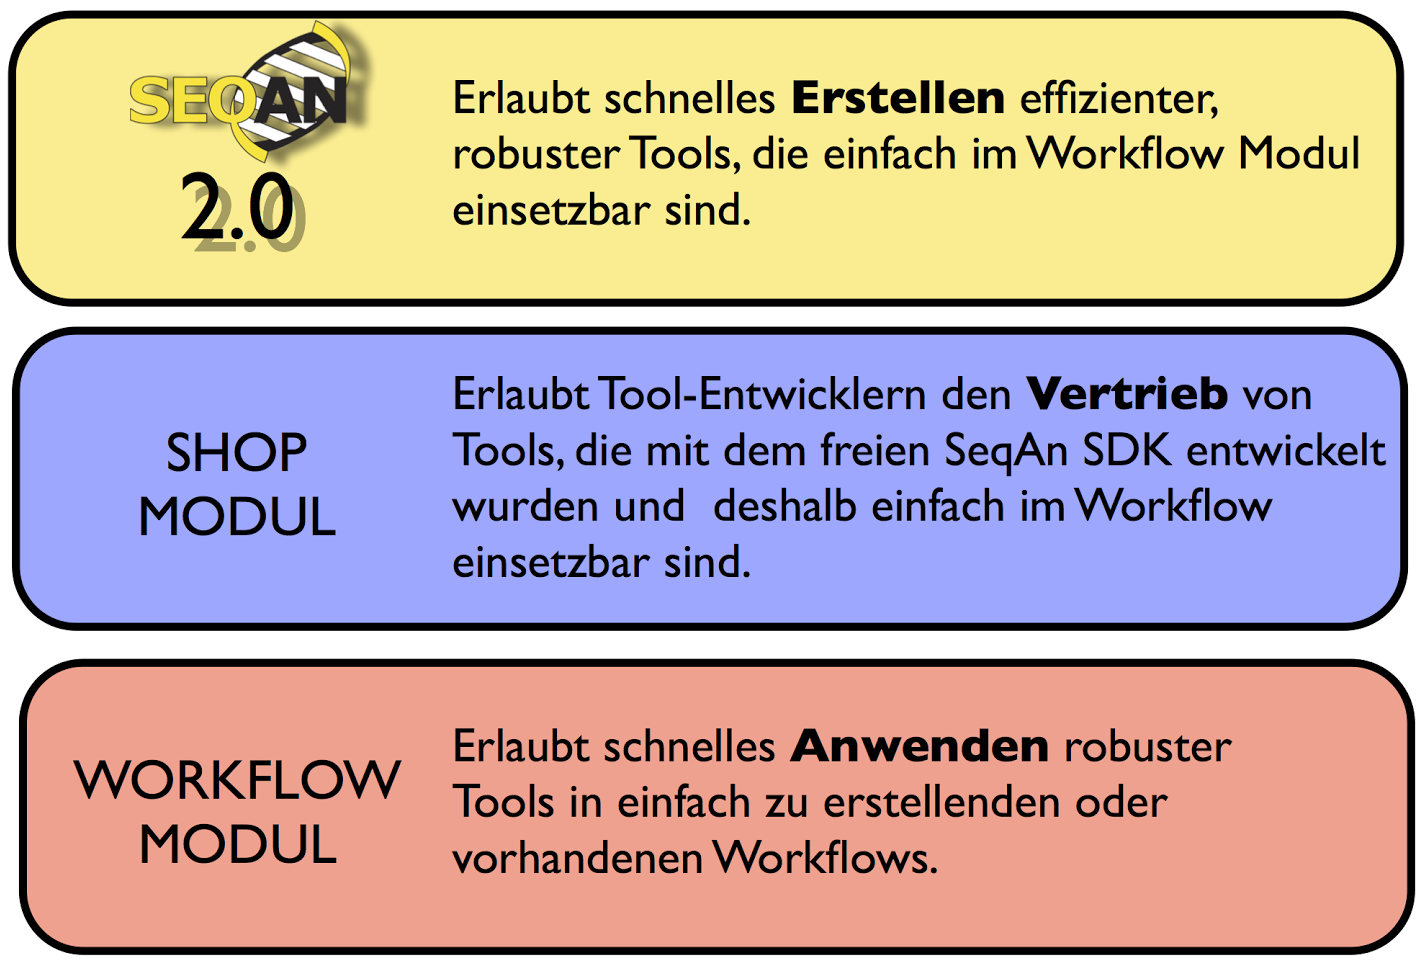
\includegraphics[width=0.6\linewidth]{Figures/seqan20.png}
  \caption[BioStore-Komponenten]{Komponenten des BioStore-Projekts \citep{Reinert:2011vl}}
  \label{fig:biostore-demonstrator}
\end{figure}

Ich besetzte innerhalb dieses Projekts die Stelle des Usability-Spezialisten, der für die Usability-Verbesserung der Softwarebibliothek SeqAn zuständig war. SeqAn spielte im Rahmen von BioStore eine primäre Rolle, da praktisch alle bereitgestellten Bioinformatik-Werkzeuge auf SeqAn basierten (siehe \sref{sec:seqan-tools}). Der zweite Schwerpunkt meiner Projekttätigkeit bestand in der Mitarbeit am BioStore selbst und am Workflow-Modul. Aus ökonomischen Gründen musste der Umfang des Projekts auf Seiten der Arbeitsgruppe gekürzt werden. Anstelle eines eigenen Shops und eines eigenen Workflow-Moduls wurde die Workflow-Engine \textit{KNIME Analytics Platform}\footnote{\url{http://www.knime.org/knime}} (kurz: KNIME) verwendet und erweitert. Die Arbeiten an KNIME fielen somit unter anderem in meinen Zuständigkeitsbereich.



\subsection{Planung}

\label{sec:data-sources-workshop}
Im Rahmen des dreijährigen BioStore-Projekts sollten drei Workshops stattfinden, die sich an Interessierte aus der Bioinformatik und verwandten Wissenschaften richteten\footnote{\url{http://www.seqan-biostore.de/wp/seqan-workshops/}}. Ziel der Workshops war es, den Anwendern SeqAn theoretisch wie auch praktisch vorzustellen und den Teilnehmern die Möglichkeit zu geben, ihre auf SeqAn-basierten Projekte vorzustellen. Für den praktischen Teil wurden vornehmlich die online-verfügbaren SeqAn-Tutorials\footnote{\url{http://seqan.readthedocs.org/en/master/Tutorial.html}} gemeinsam mit den Workshop-Teilnehmer interaktiv bearbeitet. Ein solcher Workshop bot also die ideale Möglichkeit, Forschungsdaten zur Analyse und Verbesserung der API-Usability von SeqAn im Rahmen einer explorativen empirischen Fallstudie zu erheben.

Die ursprüngliche Planung bestand aus den folgenden Phasen:

\begin{description}
  \item[1.Datenerhebung] \hfill \\
  Es war vorgesehen, objektive Daten zu erheben. Diese Daten sollten die Entwicklungsschritte der von den SeqAn-Workshop-Teilnehmern entwickelten Programme dokumentieren. Diese Datenquelle wird im Folgenden als \textit{Programmierfortschritte}-Datenquelle bezeichnet und im \sref{sec:programmierfortschritte} genauer vorgestellt.
  \item[2. Datenanalyse] \hfill \\
  Die erhobenen Daten sollten mit Hilfe der \gls{gtm} analysiert werden. Dieser Schritt sollte die vorhandenen API-Usability-Probleme nicht nur aufdecken, sondern auch ein grundlegendes Verständnis verschaffen.
  \item[3. API-Usability-Verbesserung] \hfill \\
  Auf der Grundlage der Analyseergebnisse sollten Verbesserungsvorschläge für die API von SeqAn formuliert und umgesetzt werden.
  \item[4. Validierung] \hfill \\
  Mit einer weiteren Datenerhebung und -analyse mittels \gls{gtm} sollte die Effektivität der zuvor umgesetzten Usability-Verbesserungen validiert werden. Die Verbesserungen mussten also spätestens bis zum dritten und letzten Workshop umgesetzt worden sein, um eben diesen Workshop als letzte Möglichkeit der Datenerhebung für die Validierung nutzen zu können.
\end{description}



\subsection{Tatsächlicher Verlauf}
\label{sec:verlauf}

Der zeitliche Verlauf wich stark von der ursprünglichen Planung ab. Dies ist im Grunde nicht weiter erstaunlich, ist die von mir verwendete \gls{gtm} doch ein sehr offener --- weil explorativer --- Forschungsansatz.

\label{sec:data-sources-pmsb}
Neben den SeqAn-Workshops bot sich eine weitere Datenquelle an, nämlich das jährlich stattfindende Bioinformatik-Praktikum \textit{Projektmanagement im Softwarebereich (PMSB)}\footnote{\url{http://www.mi.fu-berlin.de/w/ABI/LectureWiki}} des Fachbereichs Mathematik und Informatik der Freien Universität Berlin. Innerhalb dieses Praktikums erhalten die teilnehmenden Studenten eine 4-tägige Einführung in SeqAn, bei der die von den Workshops bekannten Tutorials eingesetzt werden. Der Einführung schließt sich eine einmonatige Projektarbeit an, bei der SeqAn zum Einsatz kommt. Drei dieser Veranstaltungen lagen in dem ursprünglich geplanten Zeitraum für diese Arbeit und boten sich so ebenfalls für die Datenerhebung an.

\bigskip

Die vier größten Schwierigkeiten bei der Einhaltung der ursprünglichen Planung waren:
\begin{description}
  \item[Organisatorische Restriktionen] Abgesehen von möglichen Langzeitbeobachtungen\footnote{Diese Datenquelle war die einzige, bei der ich hohe organisatorische Freiheitsgrad bzgl. der Durchführung hatte. Darauf gehe ich genauer im \sref{sec:phase2-programmierfortschritte-durchfuhrung} auf Seite \pageref{sec:phase2-programmierfortschritte-durchfuhrung} ein.} gab es nur die SeqAn-Workshops und die hinzugekommenen PMSB-Praktika, deren zeitliche Planung sich an anderen Faktoren orientierte als meiner Forschung. Dieser Umstand führte dazu, dass jede Möglichkeit zur Datenerhebung genutzt und so umfassend wie möglich sein musste. Schließlich erfordert die korrekte Anwendung der \gls{gtm} für die Klärung von Theorielücken weitere Datenerhebungen (\textit{theoretisches Sampling}) durchzuführen.
  \item[Unübliches Datenformat] Die Art der erhobenen Daten machte die Entwicklung eines Werkzeugs zur Datenvisualisierung notwendig. Jedoch erforderte der Einsatz der \gls{gtm} eine entsprechende technische Unterstützung. Diese Erkenntnis machte den Ausbau des Datenvisualisierungswerkzeugs zu einem qualitativen Datenanalysewerkzeug notwendig, dessen Entwicklung weit mehr Zeit in Anspruch nahm, als ich annahm. Dieses Werkzeug mit dem Namen \acrlong{apiua} stelle ich im \sref{sec:apiua} vor.
  \item[Unreife Usability] Bereits bei der Vorbereitung und Durchführung der ersten Datenerhebung und spätestens bei der Analyse dieser Daten wurde klar, dass SeqAn unter teils offensichtlichen und in der Literatur längst bekannten API-Usability-Problemen litt. Diese Probleme dominierten die Daten so stark, dass die interessanteren und fundamentaleren Probleme kaum noch zu beobachten waren oder gar nicht erst auftraten. Darum mussten die groben API-Usability-Probleme zunächst zeitraubend beseitigt werden.
\end{description}

\bigskip

Retrospektiv betrachtet ergab sich der folgende, vereinfacht dargestellte Verlauf (vgl. \fref{fig:forschung-ablauf}):

\begin{enumerate}
  \item Erste Datenerhebung (Workshop'11)\footnote{Ich verwende die Notation \textit{'xx} für die Darstellung des Jahres, in dem eine Veranstaltung stattfand. \textit{`11} steht beispielsweise für das Jahr \textit{2011}.}
  \item Implementierung eines Werkzeugs zur Datenvisualisierung / -exploration 
  \item Zweite Datenerhebung (PMSB'12)
  \item Datenanalyse (Workshop'11 und PMSB'12)\\und parallele Weiterentwicklung des Datenvisualisierungswerkzeugs zu einem Datenanalysewerkzeug, das später den Namen \textit{\gls{apiua}} erhielt
  \item Behebung grober API-Usability-Probleme
  \item Dritte Datenerhebung (Workshop'12)
  \item Literaturforschung
  \item Datenanalyse (Workshop'11 und PMSB'12)\\und bedarfsgetriebene parallele Weiterentwicklung von \gls{apiua}
  \item Vierte Datenerhebung (PMSB'13)
  \item Abschluss der Behebung grober API-Usability-Probleme\\(insbesondere Dokumentation)
  \item Fünfte Datenerhebung (Workshop'13)
  \item Datenanalyse (Workshop'13-Fragebögen)\\und bedarfsgetriebene parallele Weiterentwicklung von \gls{apiua}
  \item Datenanalyse (Workshop'12-Gruppendiskussion)
  \item Verifikation der Erkenntnisse an Hand der Datenquelle \textit{Programmierfortschritte}
  \item Synthese der Forschungsergebnisse
  \item Formulierung von API-Usability-Verbesserungsvorschlägen
\end{enumerate}

\newgeometry{inner=2cm,outer=1.5cm,top=1.5cm,bottom=1.5cm}
\thispagestyle{empty}
\begin{landscape}
\begin{figure}
  \centering
    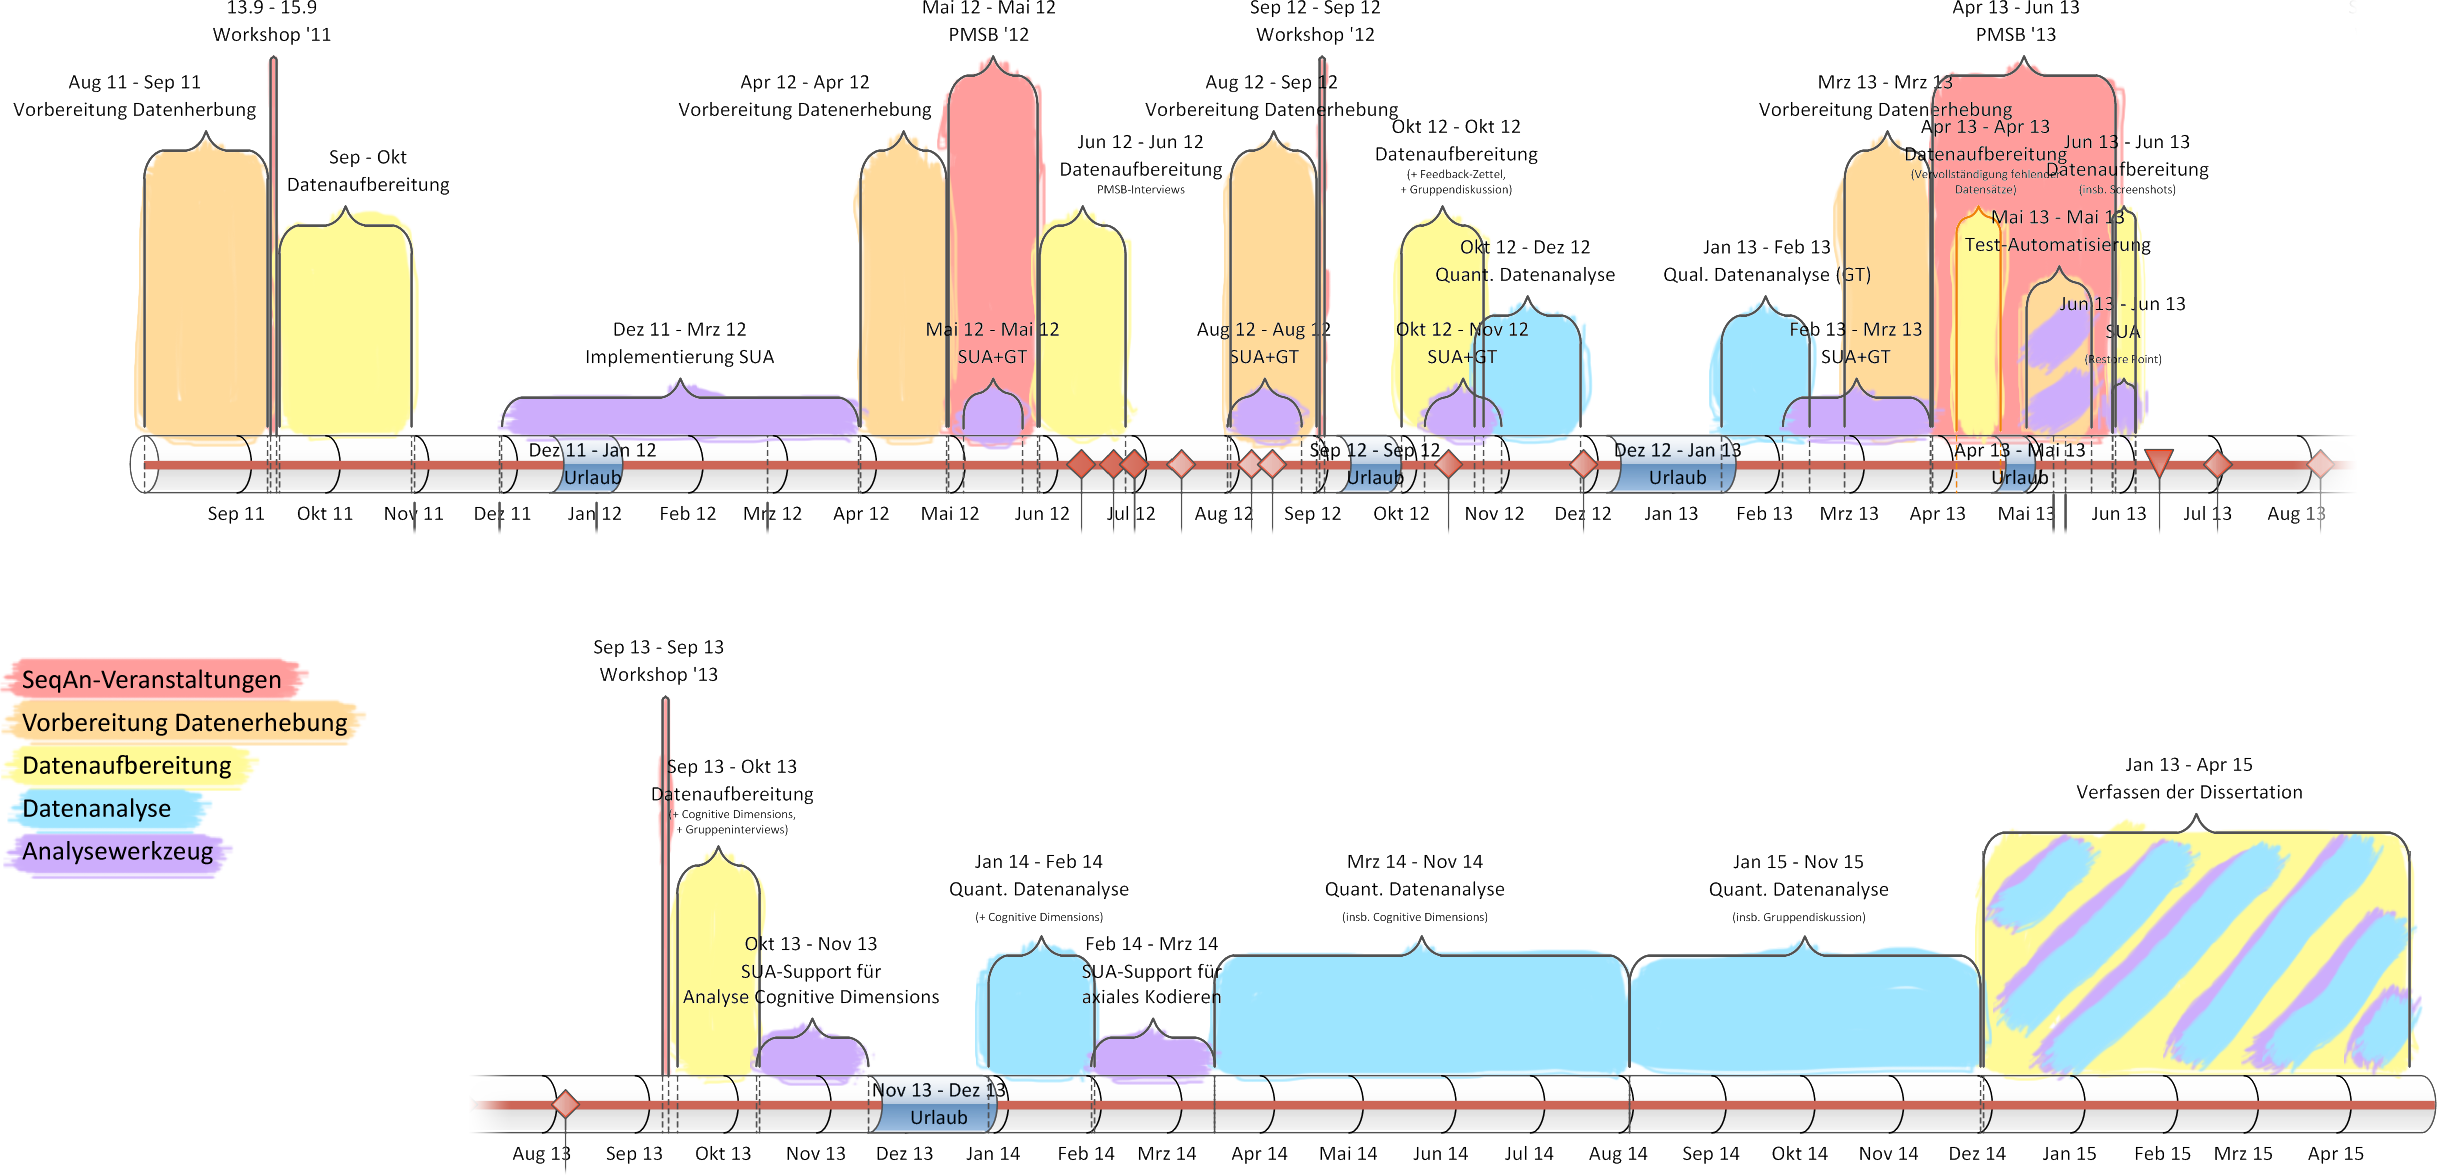
\includegraphics[width=1.0\linewidth]{Figures/forschung-ablauf.png}
  \caption[Zeitlicher Verlauf dieser Arbeit]{Zeitlicher Verlauf dieser Arbeit\\Datenerhebungen sind rot, Datenerhebungsvorbereitungen orange, Datenerhebungsnachbereitungen gelb, Datenanalysen blau und Arbeiten am Datenanalysewerkzeug violett dargestellt.}
  \label{fig:forschung-ablauf}
\end{figure}
\end{landscape}
\restoregeometry

Die zwei wichtigsten Auffälligkeiten sind einerseits die zusätzlichen Datenerhebungen während zwei PMSB-Praktika und andererseits der große Zeitbedarf der \gls{apiua}-Entwicklung.

Im Verlauf meiner Forschung stellte sich schnell heraus, dass meine Unerfahrenheit im Umgang mit der \gls{gtm}, gepaart mit der speziellen Gestalt der erhobenen Programmierfortschritte-Daten zu zeitintensiv sein würde, um das Ziel der Verbesserung der API von SeqAn zu erreichen. Ich musste zunächst Erfahrungen im Gebrauch der \gls{gtm} sammeln und meine \textit{theoretische Sensibilität} schärfen. Aus diesen Gründen entschloss ich mich, zunächst subjektive Datenquellen wie Fragebögen, Interviews und Gruppendiskussionen für die Datenerhebung zu verwenden und zu analysieren. Dieser Methodenmix hatte den Vorteil, dass ich so auch APU-Usability-Probleme aufdecken konnte, die nur in einer der Datenquellen zu finden waren. Außerdem wurde dieses Vorgehen dem Gütekriterium \textit{Triangulierung} \citep{mayring2002einfhrung} gerechter.

Aus diversen, im \href{sec:schwierigkeiten}{nächsten Abschnitt beschriebenen Schwierigkeiten} musste ich von der Planung Abstand nehmen, eine empirische Validierung der API-Usability-Verbesserungen vorzunehmen.



\subsection{Schwierigkeiten}
\label{sec:schwierigkeiten}

\subsubsection{Wissenschaftliche und methodische Schwierigkeiten}

Die Einarbeitung in das Gebiet der API-Usability war unerwartet aufwändig, da es keine umfassenden, über ``den Tellerrand'' schauenden, wissenschaftlichen Literaturstudien gab. Eine solche Literaturstudie musste ich also zunächst erarbeiten.

Diese im vorangegangen Kapitel vorgestellte \href{sec:forschungsstand}{Literaturstudie} --- insbesondere \cite{Robillard:2010bh,Eisenberg:2010bm,Stylos:2009bq,Stylos:2008jt,Ellis:2007kv} --- zeigt, dass sich die Forschung häufig nur auf kleine definierte API-Usability-Aspekte konzentrierte. Entsprechend sinnvoll war die Verwendung der sich für explorative Studien besonders geeigneten \gls{gtm}.
\\Die Verwendung der \gls{gtm} ist für einen Informatiker jedoch nicht einfach und selbst empirische Forschung findet in der Informatik wenig statt. In einer Literaturstudie von 1995-1999 fanden \cite{Glass:2002ec} heraus, dass nur ein Bruchteil der veröffentlichten Studien empirisch zu Stande gekommen ist und gerade einmal 2\% der Arbeiten Bezug auf andere Disziplinen genommen haben. Außerdem habe ich im \sref{sec:gtm-informatik} dargestellt, wie wenig Studien überhaupt die \gls{gtm} einsetzen. Unter den mit bekannten \gls{gtm}-Studien befindet sich nicht eine, die tatsächlich eine \gls{gt} vorgestellt hat. Bei der Hälfte wurde die \gls{gtm} nur in unzureichender Weise angewandt.
\\Für die Erforschung der API-Usability-Forschung mittels \gls{gtm} gibt es keine Studie, an der ich mich methodisch orientieren konnte. Entsprechend eigenständig musste ich also die Datenerhebung und -analyse individuell planen und realisieren.

Forscher, die ein gutes Verständnis von API-Usability und von ihrem fachlichen Forschungsgegenstand haben, sind rar \citep{DaqingHou:2005ba}. Dies trifft auch auf Informatik und Bioinformatik zu \citep{Tisdall:2001td}. In Bezug auf Bioinformatiker als Anwendergruppe gibt es kaum Forschung \citep{Letondal:2006dy}. Das spezielle Datenerhebungsverfahren und der ihm geschuldete Bau eines Datenanalysewerkzeugs gestaltete das Vorhaben nicht einfacher.

%Kurzum: Als Informatiker die vergleichsweise schlecht erforschte API-Usability einer auf Templatemetaprogrammierung-basierenden Bioinformatik-Softwarebibliothek mittels \gls{gtm} zu verbessern, ist kein triviales Unterfangen. 

Die oben genannten Gründe und Zeitprobleme zwangen mich zu einer kostengünstigen Validierung meiner Arbeit. Diese scheiterte jedoch an der, nicht ohne weiteres ersichtlichen Unreife des Cognitive Dimension Frameworks (siehe \sref{sec:cdf-validation-difficulties}), welches ich für diesen Zweck verwenden wollte. Darum musste ich mich gegen eine empirische und für eine argumentative Validierung entschließen. 

Auf Seiten der Bioinformatik-Arbeitsgruppe gab es andere Vorstellungen von meiner Arbeit im BioStore-Projekt. Mein Promotionsziel und den API-Usability-Forschungsstand übersehend, wurden quantitative, zeitnahe und unmittelbar umsetzbare Forschungsergebnisse erwartet. Ich führe dies auf den quantitativen Forschungsschwerpunkt der Bioinformatik, einer gewissen Unerfahrenheit mit qualitativer Forschung\footnote{Äußerungen der Mitglieder der Bioinformatik-Arbeitsgruppe in persönlichen Gesprächen, wie auch bei der Präsentation von Zwischenergebnissen gaben Aufschluss über die existierende Skepsis gegenüber und Unerfahrenheit mit qualitativer Forschung.} und auf die zeitliche Begrenzung des BioStore-Projekts zurück.



\subsubsection{Organisatorische Schwierigkeiten}

\paragraph{Aufgaben}

Häufig sind Forscher, die ein Promotionsziel verfolgen, mit der Tatsache konfrontiert, dass auch andere Aufgaben in ihren Arbeitsbereich fallen. In meinem Fall gehörten zu diesen Aufgaben die Arbeit an der Workflow-Engine KNIME, die im ersten Jahr mehrere Monate umfasste.

Die geforderten quantitativ-konstruktiven Forschungsergebnisse belasteten mich jedoch mehr, denn sie waren nicht nur zeitraubend und für meine Promotion von nur geringer Relevanz, sondern dienten auch dem Projekt nur als kosmetischer Balsam für die Entwickler-Ehre und weniger zur grundlegenden Usability-Verbesserung der SeqAn-API.
\\Ich habe die These, dass Teile der SeqAn-Entwickler von der Usability der Softwarebibliothek bereits überzeugt waren. Starke Indizien dafür sind \textit{Bauchgefühl-Usability}\footnote{Damit bezeichne ich die \textit{intuitive} (im Gegensatz zur \textit{argumentativen} oder \textit{empirischen}) Entscheidungsfindung in Bezug auf Usability-relevante Entwurfsentscheidungen. Im \sref{sec:bauch-usability} beschreibe ich dieses Konzept ausführlicher.}
und \textit{technisches Wegargumentieren}\footnote{Dieses Konzept wird von \cite{Sarodnick:2006vc} anekdotisch beschrieben. Dabei tendieren Softwareentwickler stark dazu, Eindrücken ihrer Anwenderschaft --- berechtigt oder nicht --- mit technischen Argumenten zu begegnen. Diese Erfahrung machte ich selbst bereits bei der ersten Feedback-Runde während des ersten SeqAn-Workshops. Im \sref{sec:gruppendiskussion} bespreche ich die daraus gezogenen Konsequenzen für meine Datenerhebung.}.

Es boten sich sechs Datenerhebungsmöglichkeiten (drei SeqAn-Workshops, drei PMSB-Praktika). Eine einzelne Datenerhebung forderte einen erheblichen Vor- und Nachbereitungsaufwand. Noch weitaus schwerer wog der Aufwand für die Analyse eines solchen Datensatzes. Auch wenn es illusorisch war, alle Datensätze zu analysieren, erntete ich mit meiner Entscheidung, die letzte Datenerhebungsmöglichkeit aus zeitlichen und inhaltlichen Gründen nicht mehr zu nutzen, größtenteils Unverständnis.

Meine Stellung in der Bioinformatik-Arbeitsgruppe (AGABI) war durch meine wissenschaftliche Zugehörigkeit zur Arbeitsgruppe \textit{Software Engineering} (AGSE) diffus, was sich selbst in einer Diskussion zu den Schließrechten der entsprechenden Räumlichkeiten zeigte. Dies führte in Verbindung mit meiner, eben geschilderten Unzufriedenheit zu einer unbewussten Entfernung von der AGABI, was aber auch in einen geringeren Informationsfluss mündete. 

\paragraph{Projekt}

Auf Projekt-Ebene gestaltete sich die Erarbeitung dieser Dissertation schwierig, denn das BioStore-Projekt war auf drei Jahre beschränkt --- und damit auch die Bezahlung des Personals. Dies führte zu finanziellen Problemen meinerseits. Meine Erfahrung mit anderen Kollegen zeigte mir, dass der erfolgreiche Abschluss der Promotion nur in Vollzeit möglich ist. Diese Monate musste ich mir mit meinen knappen Ersparnissen finanzieren und mich finanziell auf das Nötigste reduzieren.

Die inhaltliche Arbeit erschwerte sich durch den Projektende-bedingten Wegfall wichtiger Projektmitglieder, zu denen insbesondere zwei SeqAn-Hauptentwickler gehörten. Dadurch rutschte die Umsetzung wichtiger API-Usability-Verbesserungen in weite Ferne --- beziehungsweise in den \href{sec:ausblick}{Ausblick dieser Arbeit}. Diese Entwicklung machte die empirische Validierung dieser Verbesserungsvorschläge unmöglich.

\paragraph{Technik}

Die personelle Dynamik setzte sich in der eigentlichen SeqAn-Softwarebibliothek fort, denn sie wurde natürlich während meiner Arbeit stetig im Sinne des BioStore-Projekts funktionell (z.B. IO-Modul, Parallelisierung) und strukturell (z.B. Beseitigung von Forward-Declarations) weiterentwickelt. Zu diesen Änderungen gehörten allerdings auch eigenmächtige Bauchgefühl-Usability-Verbesserungen wie dem Wechsel der Tutorial-Dokumentationsplattform von \textit{trac}\footnote{\url{http://trac.edgewall.org}}, hin zur auf \textit{Sphinx}\footnote{\url{http://sphinx-doc.org}}-basierenden \textit{Read the Docs}-Plattform\footnote{\url{http://seqan.readthedocs.org}}.

%- Bibliotheksumstrukturierungen (Beseitigung von forward declarations, Parallelisierung (mit GPU), Herausarbeitung von Apps in eigene Github-Repositories)

Darüber hinaus hat sich sogar die, SeqAn zu Grunde liegende Programmiersprache C{}\verb!++! weiterentwickelt. Anpassungen an den C{}\verb!++!11-Sprachstandard wurden in SeqAn Mitte 2014 angefangen und mittlerweile zum Abschluss gebracht.

\bigskip

Im Folgenden werde ich eine --- von den oben genannten Schwierigkeiten weitestgehend bereinigte --- Darstellung meiner Forschung vornehmen und sie nicht rein zeitlich, sondern vornehmlich inhaltlich gliedern. Um den Lesefluss und das Verständnis dieser Arbeit nicht unnötig zu erschweren, nehme ich nur an Stellen Bezug auf diese Schwierigkeiten, wenn es der Nachvollziehbarkeit dienlich ist.
\section{Phase 1: Behebung grober API-Usability-Probleme}
\label{sec:phase1}

Die erste Einarbeitung in SeqAn und spätestens der erste \gls{gtm}-Analyseversuch der unter \ref{sec:programmierfortschritte} erläuterten \textit{Programmierfortschritte}-Datenquelle haben gezeigt, dass SeqAn teils offenkundige, schwere Usability-Probleme aufweist. Diese galt es in dieser ersten Phase zu beheben. Es bestand begründete die Befürchtung, dass derartige Probleme die Sicht auf die interessanten und tiefschürfenden API-Usability-Probleme verdecken. Insbesondere Dokumentationsprobleme, wie veraltete Installationsanleitungen, fehlende, kritische Dokumentationseinträge\footnote{U.a. waren die Konstruktoren der wohl wichtigsten Klasse --- nämlich der \texttt{String}-Klasse --- nicht dokumentiert.} und unzureichende Anwendungsbeispiele stellen starke Indizien für diese Befürchtung dar. Es ist davon auszugehen, dass derartige Lernhindernisse interessante Probleme gar nicht erst eintreten lassen. Es hat sich beispielsweise in der späteren Analyse gezeigt, dass manche Anwender bei zu großen Anfangsproblemen nicht weiter mit SeqAn arbeiten (siehe Seite \pageref{sec:gt-seqan-alternative}). Die genauen Ergebnisse dieser ersten Phase stelle ich weiter unten ab Seite \pageref{sec:phase1-ergebnisse} vor.

Um diese groben Probleme überhaupt systematisch aufzudecken, analysierte ich die Artefakte, auf die vermutlich ein Anwender trifft, wenn er das erste Mal SeqAn verwendet. Ich habe also die \textit{\gls{oobe}} \citep{Fouts:2000:SLE:353360.353375} von SeqAn mit Hilfe einer vereinfachten \textit{\glslink{he}{Heuristischen Evaluation (HE)}} analysiert.

Darüber hinaus habe ich während der ersten drei Datenerhebungsmöglichkeiten aus Triangulierungsgründen Befragungen unterschiedlicher Form durchgeführt (\textit{Workshop'11}: Online-Umfrage, \textit{PMSB'12}: Online-Umfrage und Interviews, \textit{Workshop'12}: Feedback-Zettel).

Die Datenanalyse diente, neben der Aufdeckung grober Usability-Probleme, auch der Verbesserung der SeqAn-Workshops selbst. Ein weiterer Nutzen war die Verbesserung meiner, für die Anwendung der \gls{gtm} notwendigen \textit{theoretischen Sensibilität}.



\subsection{Datenerhebung}

\subsubsection{\acrlong{oobe} relevante Artefakte}
\label{sec:oobe}

``Die \acrlong{oobe} --- kurz \acrshort{oobe} --- beschreibt die ersten Erfahrungen, die ein Anwender mit einem Produkt macht. Häufig hat der Anwender dabei --- abhängig von der Art des Produkts --- Kontakt mit den folgenden Artefakten: Produktverpackung und -handbuch, Installationsprozedur, Konfigurationsassistent, usw. \citep{Fouts:2000:SLE:353360.353375}''. \citep{Kahlert:2011wr}

Für die relevanten OOBE-Artefakte von SeqAn habe ich die Installationsanweisungen (\textit{Getting Started}), die drei Anfänger-Tutorials (\textit{Basics}, \textit{Sequences}, \textit{Iterators}) und die den SeqAn-Entwurf erklärenden Tutorials (insb. \textit{Metafunctions} und \textit{Template Subclassing}) betrachtet.

\subsubsection{Online-Umfrage}

Die Online-Umfrage hatte folgende Ziele:
\begin{description}
  \item[Vorerfahrung] Die Anwenderschaft von SeqAn sollte besser verstanden werden. Interessant waren allgemeine Programmiervorkenntnisse und spezielle Programmierkenntnisse in Bezug auf die in SeqAn eingesetzten Techniken (siehe \sref{sec:seqan-entwurf}).
  \item[Installation] Probleme bei der Installation eines Produkts sind inhärenter Bestandteil der OOBE und entsprechend auch für SeqAn von hoher Relevanz.
  \item[Tutorials] Auch die Tutorials sind wichtige OOBE-relevante Artefakte. Schließlich handelt es sich bei den Tutorials um \textit{die} Lernressource für SeqAn-Anfänger.
  \item[Bewertung] Persönliche Einschätzungen von SeqAn und dessen Gebrauch waren ebenfalls von Interesse für mich.  
\end{description}

Der vollständige Fragebogen befindet sich im \aref{app:umfrage}. Er enthält auch Fragen zur Organisation des SeqAn-Workshops, die aber nicht Gegenstand dieser Arbeit sind.

Der Fragebogen wurde unter Berücksichtigung von \cite{mayring2002einfhrung} entwickelt und mit Hilfe von \textit{LimeSurvey}\footnote{\url{https://www.limesurvey.org}} implementiert und bereitgestellt.

Die Online-Umfrage wurden im Anschluss an den praktischen Teil des Workshops'11 und nach der SeqAn-Einführung des PMSB'12-Praktikums eingesetzt.

Insgesamt nahmen 18 Teilnehmer an der Umfrage teil.


\subsubsection{Interviews}

Neben der Online-Umfrage habe ich während des PMSB'12-Praktikums mit vier Teilnehmern jeweils ein offenes Interview \citep{mayring2002einfhrung} geführt. Dabei interessierten mich Probleme, auf die die Studenten beim Gebrauch von SeqAn stießen.


\subsubsection{Feedback}
\label{sec:feedback}

Bei der Durchführung der Online-Umfrage musste ich feststellen, dass eine nicht kleine Anzahl Workshop-Teilnehmer sich nicht an der Online-Umfrage beteiligte, was auf Teilnehmerseite nachvollziehbar, aber für meine Forschung nachteilig war.

Basierend auf den Erfahrungen der beiden Online-Befragungen habe ich einen Feedback-Zettel erstellt, der um weitere Fragen ergänzt wurde. Die neuen Fragen (u.a. Motivation für Bearbeitung eines Tutorials; Anwendungsform von SeqAn) bezweckten ein besseres Verständnis der SeqAn-Anwendergruppe.

Des Weiteren habe ich den Befragungsmodus geändert. Statt eine Befragung am Ende des gesamten dreitägigen Workshops durchzuführen, sollte je ein Fragebogen am Anfang der des Workshops, im Anschluss an jedes Tutorial und am Ende des Workshops ausgefüllt werden.

Die drei Feedback-Fragebogen-Varianten (Einstieg, Tutorial, Abschluss) befinden sich vollständig im \aref{app:feedback}.

Insgesamt wurden 210 Feedback-Zettel von max. 58 Entitäten ausgefüllt. Die genaue Anzahl der Beteiligten kann nicht bestimmt werden, da nicht jeder Teilnehmer seine Feedback-Zettel mit einem selbst gewählten Pseudonym markiert hat (Details siehe \sref{sec:id}). Dadurch konnten die verschiedenen Feedback-Zettel nicht einer Person zugeordnet werden und mussten separat analysiert werden.


      
\subsection{Datenanalyse}
\label{sec:he}

Für die Analyse der eben beschriebenen Daten habe ich, neben einfachen quantitativen Mitteln (vgl. \sref{sec:schwierigkeiten}), die \acrfull{he} eingesetzt.

Die \gls{he} wurde erstmalig von \cite{Nielsen:1990bw} und praxisbezogener von \cite{Nielsen:1994tx,Nielsen:1993vk} beschrieben. Sie wird dem \textit{Discount-Usability-Engineering} zugesprochen \citep{Sarodnick:2006vc}; stellt also ein kostengünstiges Verfahren zur Usability-Evaluation dar. Das Verfahren sieht vor, dass Usability-Experten Artefakte eines Softwaresystem mit der Perspektive des Anwenders gedanklich verarbeiten und dabei Verstöße gegen die vorher definierten Heuristiken aufdecken. Heuristiken haben ihren Namen von der Tatsache, dass ein Verstoß nur auf ein Usability-Problem hindeutet, es jedoch nicht beweist und die Heuristiken auch nicht alle existierenden Probleme aufdecken.

Dem ursprünglichen Verfahren liegen zehn Heuristiken zu Grunde, die ich im \aref{app:heuristiken} aufführe. 

Beim Versuch, die originären Heuristiken anzuwenden, stellte ich fest, dass sie sich nicht für die Evaluation meiner Artefakte eignen. Das betrifft insbesondere die Heuristiken \textit{Sichtbarmachung des Systemstatus}, \textit{Benutzerkontrolle und -freiheit}, \textit{Wiedererkennen, statt sich erinnern}, \textit{Flexibilität und Effizienz der Benutzung} und \textit{Ästhetik und minimalistisches Design}. Der Grund: Diese Heuristiken haben einen starken Bezug auf grafische Benutzeroberflächen, die es im Falle von SeqAn nicht gibt. Natürlich kann man Elemente von APIs beispielsweise unter ästhetischen Gesichtspunkten betrachten. Dass eine geringe Ästhetik jedoch ein hinreichend sicher auf ein Usability-Problem hindeutet, ist nicht empirisch gezeigt und stellt damit auch keine praktikable Heuristik dar.   

An dieser Stelle stand ich also vor der Wahl, speziell für die Evaluation von APIs geeignete Heuristiken herzuleiten oder lediglich die verbliebenen Heuristiken zu verwenden und mich auf meine \gls{he}-Anwendungserfahrung  \citep[vgl.][]{Kahlert:2011wr} zu verlassen. Ich habe mich für die zweite Variante aus den folgenden Gründen entschieden:

\begin{enumerate}
  \item Die theoretische bzw. literaturbasierte Herleitung von Heuristiken entspricht nicht meiner Vorstellung von explorativer Forschung. Ich befürchtete, dass eine zu intensive Auseinandersetzung mit API-relevanten Heuristiken meine \gls{gtm}-Forschung --- insbesondere beim offenen Kodieren --- verzerren und die in den Daten verankerte Theorie nicht mehr korrekt wiedergeben würde.
  \item Für einen speziellen Untersuchungsgegenstand individuelle Heuristiken zu entwickeln, ist nicht trivial \citep{Nielsen:1993vk}. Die von \cite{Grill:2012jm} entwickelten API-Heuristiken wurden erst nach meiner Analyse veröffentlicht. Allerdings sehe ich das Zustandekommen dieser Heuristiken kritisch (siehe \sref{sec:grill-kritik}.
  \item Die Bereinigung der groben Usability-Probleme stellte ``nur'' ein notwendiges und vor allem unvorhergesehenes Übel dar. Da ich mich mit der \gls{he} gut auskenne und es nicht um die Kategorisierung, sondern um die Beseitigung von Problemen ging, habe ich mir die mühsame Problem-Klassifikation erspart.
\end{enumerate}




\subsection{Ergebnisse}
\label{sec:phase1-ergebnisse}

Die Ergebnisse meiner \gls{he} sind vollständig im \aref{app:he-ergebnisse} beschrieben. Insgesamt habe ich 59 Usability-Probleme gefunden, von den 32 schwer oder katastrophal\footnote{\cite{Nielsen:1994tx} formulieren die folgenden Fatalitäten:\\0 = \textit{Kein Usability-Problem}, 1 = \textit{Kosmetisch}, 2 = \textit{Gering}, 3 = \textit{Schwer}, 4 = \textit{Katastrophal}.} waren. Im Folgenden beschränke ich mich auf die Darstellung der wichtigsten Ergebnisse.

Die Auswertung habe ich ursprünglich in \textit{Apple Numbers} vorgenommen (siehe \fref{fig:analysis-keynote}) und später auf \textit{Wolfram Mathematica} umgestellt.
%TODO: Screenshot von Datei auf rugi.imp.fu-berlin.de

\begin{figure}
  \centering
    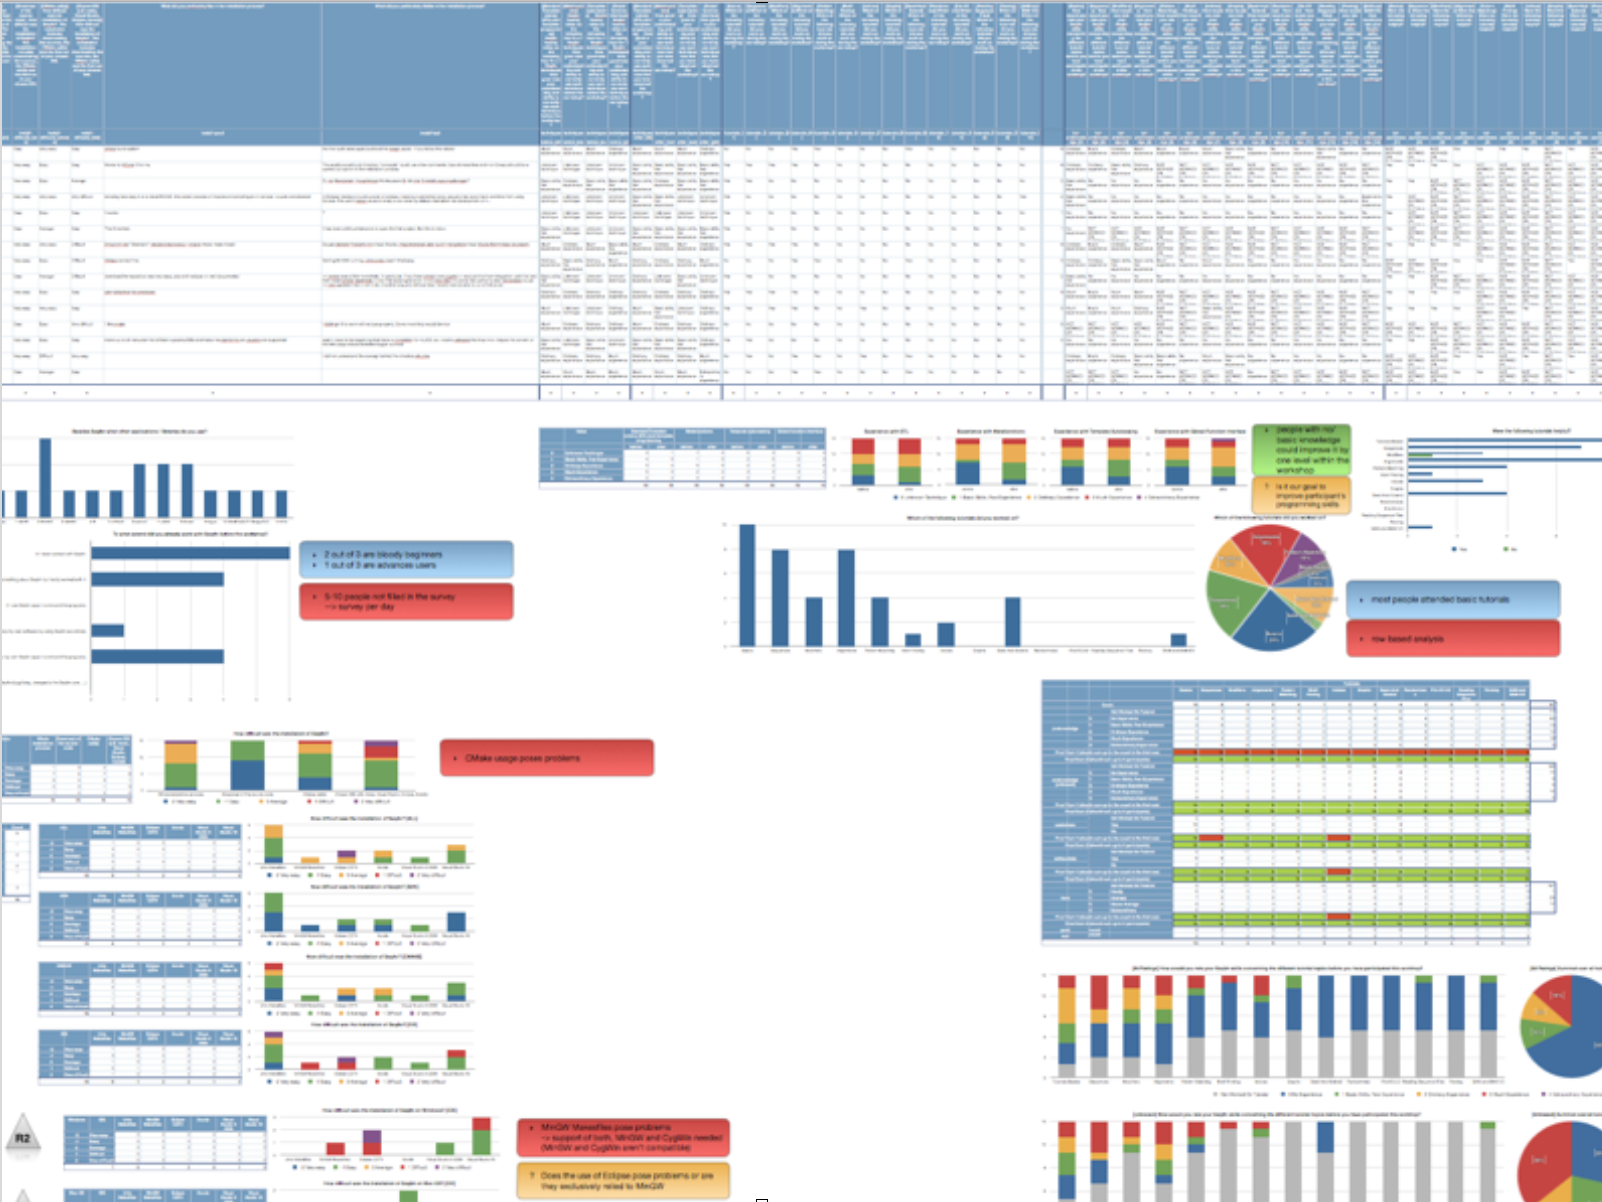
\includegraphics[width=0.75\linewidth]{Figures/analysis-keynote.png}
  \caption{Erste Analyse in Apple Keynote}
  \label{fig:analysis-keynote}
\end{figure}


\subsubsection{Anwender}
\label{sec:results-users}

Die Anwendergruppen habe ich qualitativ und quantitativ analysiert. Die Anzahl der betrachteten Anwender beträgt 35. Wegen diese geringe Anzahl, dem Workshop-Format und der subjektiven Einschätzung der Anwender selbst, kann man nicht davon ausgehen, dass die Ergebnisse verallgemeinerbar sind. Dennoch geben sie einen plausiblen Anhaltspunkt für die Charakterisierung der Anwenderschaft.

\begin{itemize}
  \item In gleichen Teilen waren Studenten und berufstätige Wissenschaftler vertreten.
  \item Jeweils knapp die Hälfte der Teilnehmer kam aus der Bioinformatik und Informatik. Aus der Biotechnologie, der Molekularbiologie und der Physik kamen jeweils einer der 35 Teilnehmer.
  \item Häufig wurden ``Effizienz'', ``Geschwindigkeit'' und ``Performance'' als Motivation zur Auseinandersetzung mit SeqAn formuliert.
  \item Etwa die Hälfte der Anwender nutzt \textit{Microsoft Windows}, ein Drittel \textit{Linux} und die übrigen \textit{Mac OS X}.
  \item Die Hälfte der Anwender nutzte eine integrierte Entwicklungsumgebung. Die andere Hälfte nutzte Makefiles.
  \item Mehr als zwei Drittel der Teilnehmer verfügt über fortgeschrittene Kenntnisse im Gebrauch von objektorientierter Programmierung in den Sprachen C{}\verb!++! oder Java.
  \item C{}\verb!++!-Kenntnisse sind gleich verteilt (jeweils ein Drittel Anfänger, Fortgeschrittene und Experten).
  \item Erfahrungen in Bezug auf den von SeqAn eingesetzten Techniken waren wenig vorhanden (Beispiel \textit{Metafunktionen}: nur 20\% fortgeschrittene Kenntnisse oder besser).
  \item Einige Anwender gaben an, dass sie von der SeqAn-Installation abgeschreckt waren. Hätten sie nicht am Workshop teilgenommen, hätten sie die Installation abgebrochen und sich nach einer anderen API umgesehen. Diese Beobachtungen machten auch \cite{sunshine2014searching}.
\end{itemize}



\subsubsection{Dokumentation}

\begin{itemize}
  \item 2 von 3 Befragten hielten die Dokumentation für mangelhaft beschrieben (vgl. \fref{fig:dox-index-old}).
  \item Den Befragten fehlten vor allem eine Einführung, Beispiele und Verlinkungen zu den Tutorials.
  \item Eine Begründung und Motivation für die Entscheidung, Templatemetaprogrammierung einzusetzen, fehlt.
  \item Es fehlen Best-Practise-Beschreibungen (z.B. \texttt{++var} oder \texttt{var++}?).
  \item Es fehlt die Beschreibung von Benennungsregeln/-konventionen für Variablen, Funktionen, etc.
\end{itemize}

\begin{figure}
  \centering
    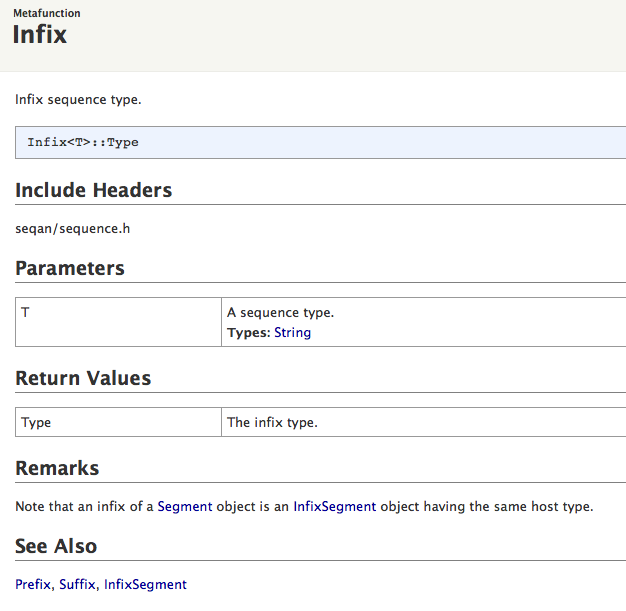
\includegraphics[width=0.95\linewidth]{Figures/dox/infix-old.png}
  \caption[Mangelhafter Dokumentationseintrag]{Mangelhafter Dokumentationseintrag zur Metafunktion \texttt{Infix},\\Stand: 02.07.2012}
  \label{fig:dox-index-old}
\end{figure}


\subsubsection{Tutorials}

\begin{itemize}
  \item Die Tutorials haben einen zu hohen Anspruch.
  \item Die Tutorials sind von geringer didaktischer Qualität.
  \item Die Tutorials verfügen über keinerlei explizite Meta-Angaben wie Zielgruppe, Schwierigkeitsgrad, etc.
  \item Die Qualität der Tutorials variiert eklatant.
\end{itemize}



\subsubsection{Installation}

\begin{itemize}
  \item Die Installation wurde mehrheitlich als schwierig beschrieben.
  \item Hauptgrund 1: Mängel in der Installationsanleitung (inkonsistent, fehlerhaft)
  \item Hauptgrund 2: SeqAn hat sich als Framework und nicht als Softwarebibliothek entpuppt. Dieser Punkt wird ausführlicher im \sref{sec:library-vs-framework} erläutert.
\end{itemize}



\subsubsection{Softwarebibliothek}

\begin{itemize}
  \item Den Anwendern war nicht klar, weshalb SeqAn die ``komplizierte'' Templatemetaprogrammierung verwendet. Die Mehrheit der Teilnehmer erwartete, dass SeqAn auf Objektorientierung basiert. Ein Teilnehmer bezeichnete SeqAn sogar als ``Vergewaltigung der OO-Programmierung''\citepurl{apiua://survey/2011-09-14-T15:23:17.211+02:00}. Dieser Punkt hat sich als äußerst relevant herausgestellt und wird u.a. im \sref{sec:lie-oop} besprochen.
  \item Die \mintinline{cpp}{length}-Funktion gibt alle Eingaben, für die sie nicht explizit entwickelt wurde, \texttt{1} zurück.
  \item Es wurden mehrere funktionale Schwächen gefunden. Beispiel: Die Konkatenierung eines SeqAn-Strings und eines C{}\verb!++!-Strings war nicht mit dem \texttt{+}-Operator möglich.
  \item Funktionen sind nur schwer aufzufinden, denn sie gehören keiner Klasse an.
  \item Mehrfach wurde das Fehlen der \texttt{substring}-Funktion zur Erzeugung von Teilstrings, bemängelt.
\end{itemize}

All die hier genannten Punkte sind von großer Relevanz, wie die spätere \gls{gtm}-Analyse gezeigt hat.



\subsubsection{Zusammenfassung der Ergebnisse}

Mit meiner Analyse der OOBE-Artefakte und den, in zwei SeqAn-Workshops und einem PMSB-Praktikum erhobenen Daten konnte ich zu einer besseren Charakterisierung der SeqAn-Anwendergruppe beitragen und teilweise schwerwiegende Probleme in der Dokumentation, den Tutorials, sowie bei der Einrichtung und bei dem Gebrauch von SeqAn aufdecken.

Als größtes Usability-Problem hat sich die Erlernbarkeit von SeqAn herausgestellt. Es gibt Indizien dafür, dass diese Anwender von der Verwendung von SeqAn abschrecken. Das Usability-Problem hat zwei Ursachen:
\begin{enumerate}
  \item Die Dokumentation ist von vergleichsweise geringer Qualität, die bei den verschiedenen Dokumentationseinträgen variiert.
  \item SeqAn setzt auf das Programmierparadigma Templatemetaprogrammierung. Dies stellt Anwender mit C{}\verb!++!-Vorerfahrung vor das Problem, dass dieser Ansatz sich stark von der C{}\verb!++! Standard (Template) Library unterscheidet. Anwender mit Java-Vorerfahrung vermissen die Ähnlichkeit zur objektorientierten Softwareentwicklung.
\end{enumerate}

Das Problem der Erlernbarkeit spielt eine wichtige Rolle im späteren Teil dieser Arbeit. Die Behebung vieler anderer Probleme wird im folgenden Abschnitt vorgestellt.





\subsection{Verbesserungen}

Jedes Usability-Problem isoliert zu lösen, ist aus praktischer Sicht weder möglich noch effizient. Viel mehr Sinn macht es, Maßnahmen zu formulieren, die eine ganze Gruppe von Usability-Problemen beheben.

Für die Behebung der gefundenen Usability-Probleme, habe ich Maßnahmen definiert und eine Maßnahmen-Probleme-Zuordnung vorgenommen. Den Aufwand einer jeden Maßnahme habe ich in Stunden geschätzt. Der Nutzen einer Maßnahme wiederum, ergibt sich aus der Anzahl und der \textit{Fatalität} der durch sie behobenen Usability-Probleme.

Zu den wichtigsten formulierten Maßnahmen gehören:
\begin{itemize}
\itemsep1pt\parskip0pt\parsep0pt
  \item Vollständige Überarbeitung und Vereinheitlichung der Installationsanleitungen
  \item Definition von Anforderungen für Tutorials
  \item Bereitstellung einer Vorlage für Tutorials
  \item Anpassung sämtlicher Tutorials an Anforderungen und Vorlage
  \item Erstellung eines neuen Anfänger-Tutorials
  \item Einführung von Aliassen in der Dokumentation (Auffindbarkeit von Einträgen durch Synonyme)
\end{itemize}

Die vollständige Zuordnung, samt der Kosten-/Nutzen-Schätzungen, befindet sich im \aref{app:he-massnahmen}. Es wurden vornehmlich die Arbeitspakete umgesetzt, die nicht die Softwarebibliothek im engeren Sinne selbst betreffen. Für die Verbesserung der Softwarebibliothek selbst sollte die, im \sref{sec:phase4} beschriebene Phase 4 dienen.

\bigskip

Im Folgenden stelle ich die tatsächlichen Änderungen vor. Meine organisatorischen und inhaltlichen Verbesserungen der SeqAn-Workshops sind nicht Gegenstand dieser Arbeit und werden daher nicht vorgestellt. 


\subsubsection{Prozessverbesserungen}

\paragraph{Commit-Nachrichten}

Die SeqAn-API-Entwickler haben ihre Commit-Nachrichten für ihr Versionsverwaltungssystem nach Belieben formuliert. Diese erschwerte die Nachvollziehbarkeit von Code-Änderungen für die Entwicklerkollegen. Für mich war dieses Format ebenso wichtig, da ich für meine Analyse darauf angewiesen war, wichtige Änderungen des SeqAn-Codes zu erfahren (vgl. \sref{sec:schwierigkeiten}). Allein für den Versionssprung von SeqAn 1.3 auf 1.4 gab es rund 3.500 Commits.

Zu Vereinheitlichung haben mein Kollege Manuel Holtgrewe und ich ein Format entwickelt, das ausführlich online\footnote{\url{http://seqan.readthedocs.org/en/master/HowTo/WriteCommitMessages.html}} beschrieben wird. Darüber hinaus habe ich einen positiv angenommenen ``Spickzettel'' (siehe \fref{fig:commit-messages-format}) erarbeitet, auf den API-Entwickler zurückgreifen können.

\begin{figure}
  \centering
    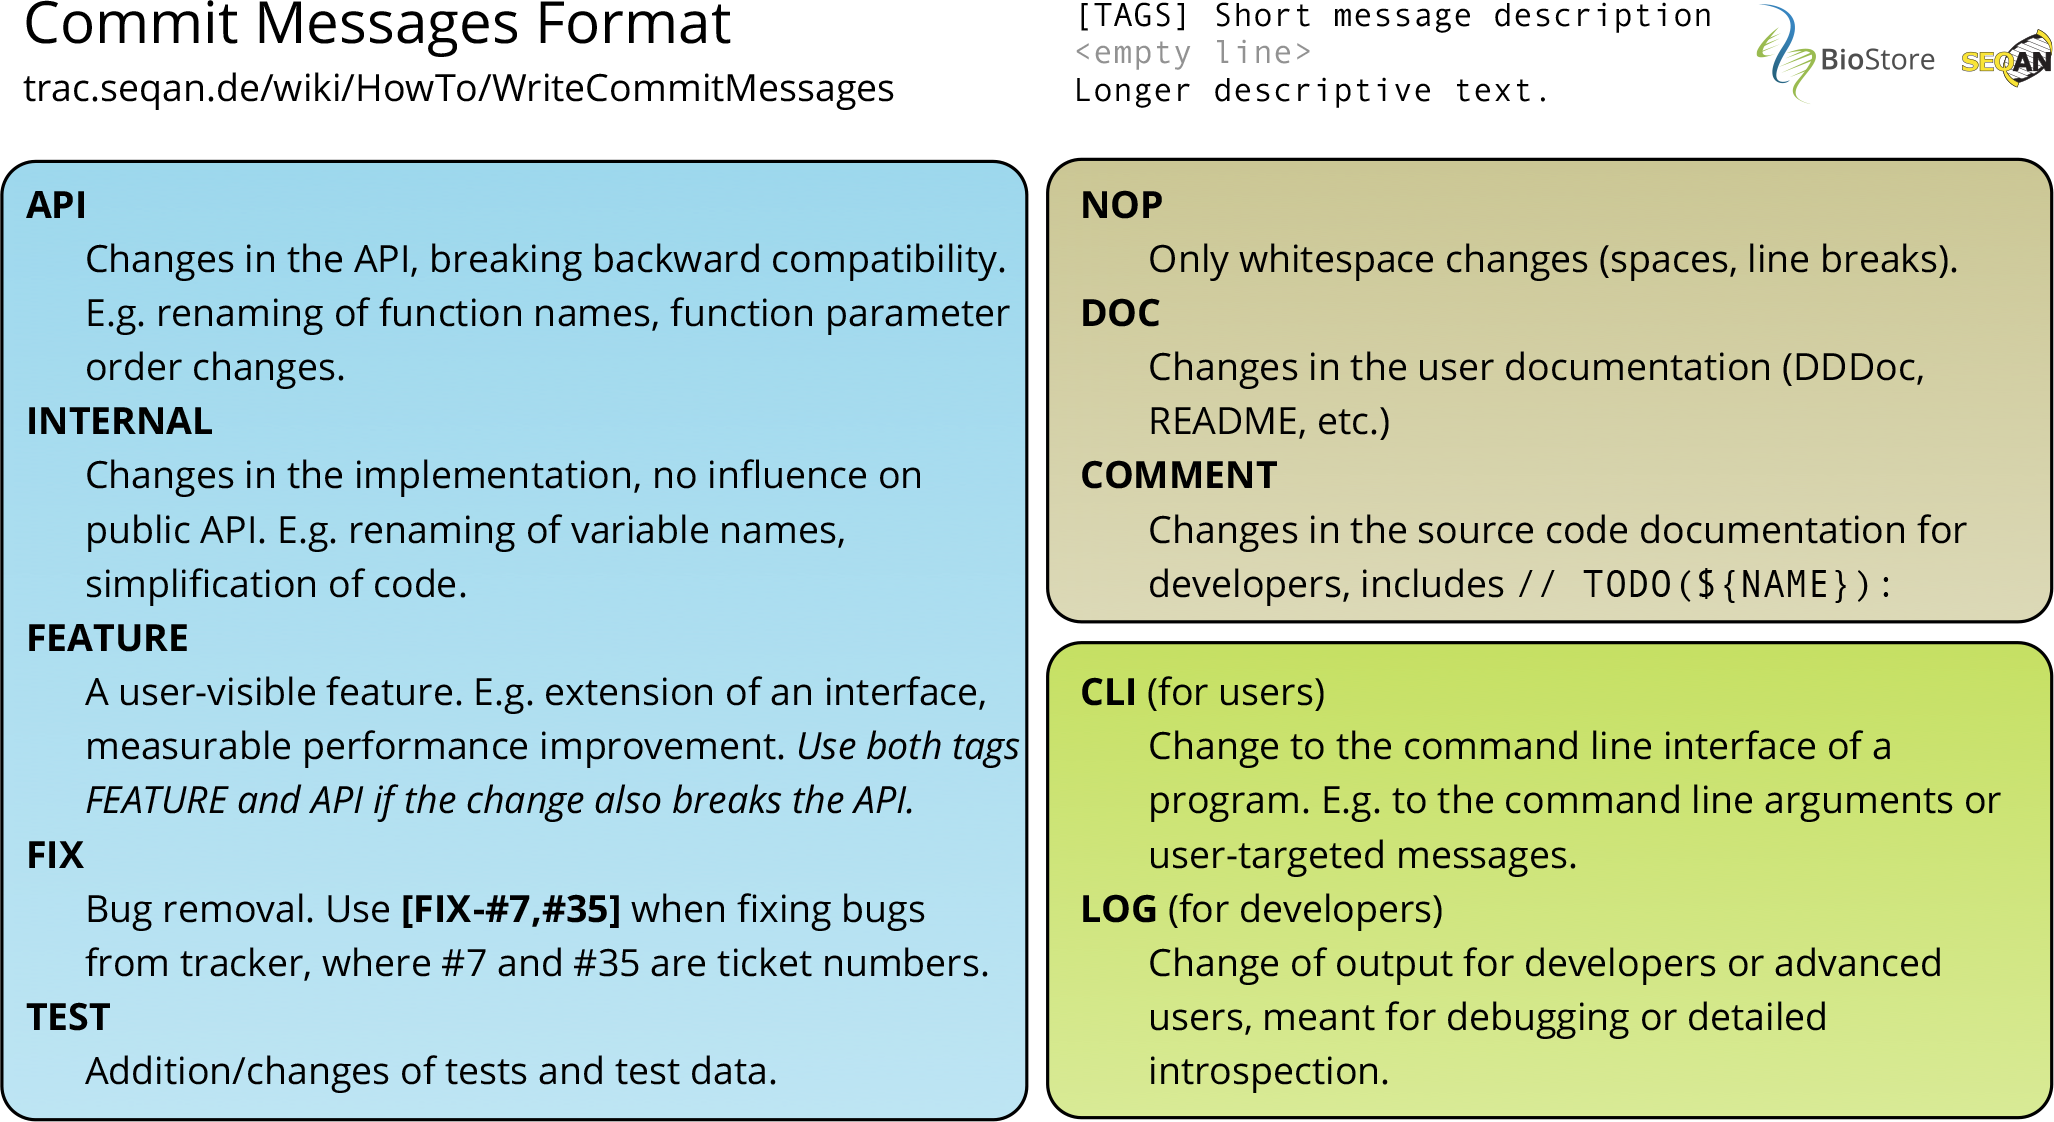
\includegraphics[width=0.9\linewidth]{Figures/20120504-CommitMessagesFormat.png}
  \caption[Commit-Nachrichten-Format]{Standardisiertes Format für Commit-Nachrichten}
  \label{fig:commit-messages-format}
\end{figure}


\paragraph{Umstellung Subversion auf Git}

In der Bioinformatik-Arbeitsgruppe arbeiten viele Mitarbeiter an einer einzigen SeqAn-Anwendung im Rahmen ihrer Tätigkeit. Dies führte durch den Gebrauch des zentralen Versionsverwaltungssystems \textit{Subversion} dazu, dass SeqAn nach dem Commit von Codeänderungen nicht mehr kompilierte.

Um SeqAn-Entwicklern eine größere Freiheit und Sicherheit zu geben, indem sie Änderungen lokal revisionieren können, wurde eine Umstellung auf \textit{Git} vorgenommen. Im Zuge dieser Umstellung wurden die Kollegen geschult und ein SeqAn-Git-Workflow\footnote{\url{http://seqan.readthedocs.org/en/master/Infrastructure/SeqAnWorkflow.html}} basierend auf dem prominenten Gitflow\footnote{\url{https://www.atlassian.com/git/tutorials/comparing-workflows/gitflow-workflow}} formuliert und etabliert.



\paragraph{Code-Reviews}

Die Entwicklung von SeqAn-Code unterlag keiner praktischen Qualitätssicherung. Aus diesem Grund habe ich angeregt, Codeinspektionen (\textit{Code-Reviews}) durchzuführen.

Diese Qualitätssicherungsmaßnahme wurde schließlich in den Commit-Prozess als Prä-Commit-Review integriert. Durch die spürbare Verlangsamung des Entwicklungsprozesses, haben die SeqAn-Entwickler, im Zuge der Git-Umstellung, auf das Post-Commit-Review gewechselt. Das heißt, Commits werden nun erst inspiziert, wenn sie bereits in den Code integriert wurden. Für externe Entwickler gilt weiterhin ein Prä-Commit-Verfahren, das durch die Arbeitsweise von Git leicht zu implementieren war.




\subsubsection{Argument-Parser}
\label{sec:argument-parser}
Für die sich vornehmlich an Wissenschaftler richtende Workflow-Engine KNIME wurde basierend auf einer Vorarbeit der Universität Tübingen\footnote{\url{http://www.knime.org/files/ugm2013_talks/knime_ugm_2013_knutreinert_final.pdf}} ein generischer Wrapper für Konsolenanwendungen zur Bereitstellung von SeqAn-Awendungen in KNIME entwickelt\footnote{\url{https://github.com/genericworkflownodes}}.

Dieser, unter dem Namen \textit{GenericWorkflowNodes} firmierende Wrapper nutzt ein XML-basiertes Datenformat zur Beschreibung seiner Ein- und Ausgabeschnittstelle. Konsolenanwendungen verfügen selbst bereits auch schon über eine beschriebene Schnittstelle, auch wenn diese nur --- möglicherweise über das ganze Programm verstreut --- programmatisch beschrieben ist.

Um eine redundante Schnittstellenbeschreibung --- nämlich einmal im Programm und einmal in der KNIME-Knotenbeschreibung --- zu vermeiden, wurde eine neue Komponente zum Parsen von Argumenten geschrieben. Diese kann sowohl die Hilfebeschreibung einer Konsolenanwendung mittels des Parameters \texttt{--help} bzw. \texttt{-h}, eine Manpage, eine HTML-Dokumentation, als auch eine  KNIME-Knotenbeschreibunsdatei ausgeben.

Dieser Argument-Parser wurde in der ersten Version von mir und später von meinem Kollegen Stephan Aiche weiterentwickelt und perfektioniert. Der Parser unterstützt ein breites Spektrum an Funktionen, das von zahlreichen Parametertypen (\textit{flag options}, \textit{value options}, \textit{positional options}, \ldots) bis hin zu Restriktionen (Typisierung, Wertebereiche, Datentypen, \ldots) reicht.

Sämtliche SeqAn-Anwendungen wurden an den neuen Argument-Parser angepasst. Dessen Verwendung stellt eine API-Usability-Verbesserung sowohl für API-Entwickler als auch für API-Anwender dar.

\bigskip

\begin{samepage}
API-Entwickler profitieren von einer einfachen, mächtigen Komponente zur Beschreibung der Schnittstelle (siehe \lref{lst:argparser-interface}) und dem Beziehen von Parametern.

\begin{center}
\begin{minted}[linenos, firstnumber=1]{cpp}
seqan::ArgumentParser parser("Argument-Parser Demo");

setShortDescription(parser, "Basic functionality of the Argument-Parser");
setVersion(parser, "0.1");
setDate(parser, "2013-09-18");

addUsageLine(parser, "[OPTIONS] \"TEXT\"");
addDescription(parser, "This program allows simple string repetition by i times.");

addSection(parser, "Demo Options");
addOption(parser, seqan::ArgParseOption("i", "times", "Number of repetitions.", seqan::ArgParseArgument::INTEGER, "INT"));

setDefaultValue(parser, "times", 1);
addTextSection(parser, "Examples");
addListItem(parser, "modify_string -i 5 \"text\"", "Print \"text\" 5 times");
\end{minted}
\captionof{listing}{Argument-Parser: Beispielhafte Schnittstellenbeschreibung in C\texttt{++}}
\label{lst:argparser-interface}
\end{center}
\end{samepage}

\bigskip

\begin{minipage}{\textwidth}
API-Anwendern stehen nun einheitlich und ausführlich beschriebene Hilfeseiten zur Verfügung (siehe \lref{lst:argparser-help}). Fehlerhafte Eingabedaten werden besser erkannt und ausführlicher zurückgemeldet (siehe \lref{lst:argparser-error}).

\begin{center}
\usemintedstyle{bw}
\begin{minted}[linenos=false]{sh}
Argument-Parser Demo - Basic functionality of the Argument-Parser
=================================================================

SYNOPSIS
    demo [OPTIONS] "TEXT"

DESCRIPTION
    This program allows simple string repetition by i times.

    -h, --help
          Displays this help message.
    --version
          Display version information

  Demo Options:
    -i, --times INT
          Number of repetitions. In range [1..100]. Default: 1.
    -O, --output-file OUT
          Path to the output file Valid filetype is: txt.

EXAMPLES
    modify_string -i 5 "text"
          Print "text" 5 times
    modify_string "text" --output-file out.txt
          Print "text" once in file out.txt

VERSION
    Argument-Parser Demo version: 0.1
    Last update 2012-08-30
\end{minted}
\captionof{listing}{Argument-Parser: Beispielhafte Hilfeseite}
\label{lst:argparser-help}
\end{center}
\end{minipage}

\bigskip

\begin{minipage}{\textwidth}
\begin{center}
\usemintedstyle{bw}
\begin{minted}[linenos=false]{sh}
demo$ ./demo -i no_int
Argument-Parser Demo: the given value 'no_int' cannot be casted to integer
\end{minted}
\captionof{listing}{Argument-Parser: Beispielhafte Fehlerausgabe}
\label{lst:argparser-error}
\end{center}
\end{minipage}



\subsubsection{Installationsanleitungen}

Die Installationsanleitungen waren fehlerhaft, uneinheitlich, unstrukturiert und verfügten über zu wenig Beispiele, um den Anleitungen folgen zu können.

Ich habe eine inhaltliche und grafische Vorlage für die plattformabhängigen Installationsanleitungen (\textit{Linux --- Makefiles}, \textit{Linux --- \gls{eclipse}}, \textit{Mac OS X --- Makefiles}, \textit{Mac OS X --- Xcode} und \textit{Windows --- Visual Studio}) erstellt.

Die von mir formulierte Gliederung lautet:
\begin{enumerate}
\itemsep1pt\parskip0pt\parsep0pt
  \item Prerequisites --- Was bereits installiert sein muss + Verlinkungen
  \item Install --- Die eigentliche SeqAn-Installation
  \item A First Build --- Überprüfung, ob Installation korrekt verlief
  \item Hello World! --- Skelett für erste SeqAn-Anwendung
  \item Further Steps --- Verlinkungen auf Dokumentation und Tutorials
\end{enumerate}

Sämtliche Installationsanleitungen wurden korrigiert, vereinheitlicht und zentral verlinkt\footnote{\url{http://seqan.readthedocs.org/en/master/Tutorial/GettingStarted.html}}. \fref{fig:getting-started-windows} zeigt einen Ausschnitt aus der Installationsanleitung für Windows.

\begin{figure}
  \centering
    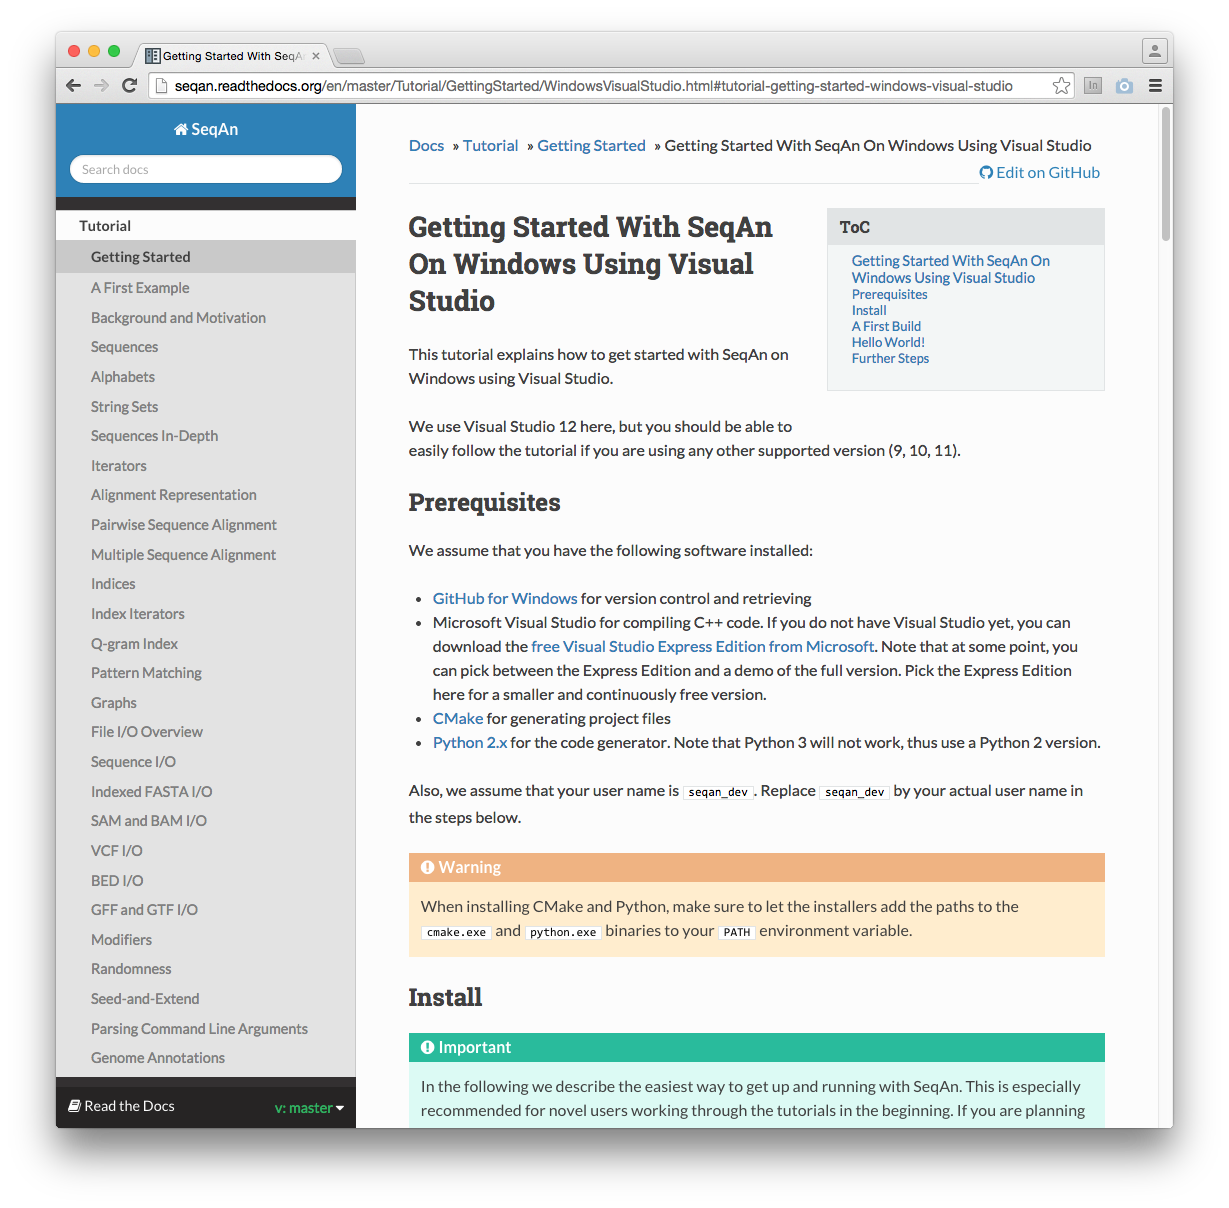
\includegraphics[width=1.0\linewidth]{Figures/getting-started-windows.png}
  \caption[SeqAn-Installation unter Windows]{Ausschnitt aus der verbesserten SeqAn-Installationsanleitung für Windows}
  \label{fig:getting-started-windows}
\end{figure}



\subsubsection{Dokumentation}

Die Dokumentation wurde über mehrere Iterationen hinweg verbessert. In die Verbesserung flossen neben den hier besprochenen Ergebnissen, insbesondere die im \sref{sec:gt} vorgestellten Ergebnisse der \gls{gtm}-Analyse. Daher wird die überarbeitete Dokumentation ausführlich im \sref{sec:improve-dox} vorgestellt.

Die Abbildungen \ref{fig:dox-index-compare-old} und \ref{fig:dox-index-compare-new} geben einen Eindruck über den Grad der Verbesserung.

\begin{figure}
        \centering
        \begin{subfigure}{0.48\linewidth}
                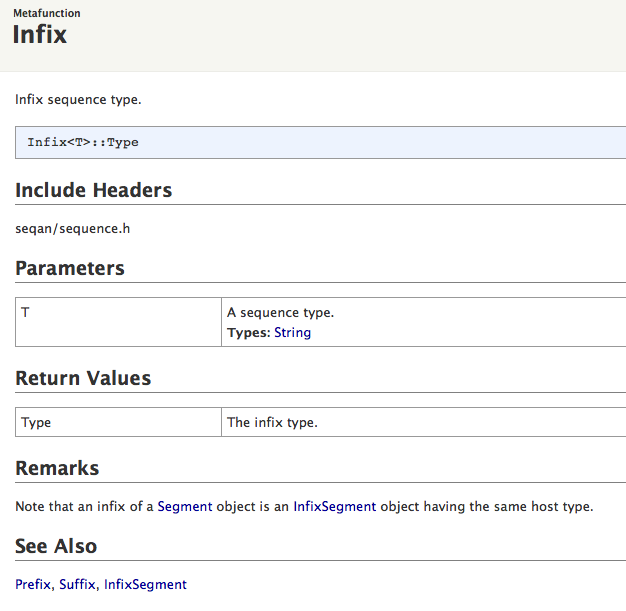
\includegraphics[width=\linewidth]{Figures/dox/infix-old.png}
                  \caption[Vergleich Dokumentationseintrag \texttt{Infix} - Alt]{Alt, Stand: 02.07.2012}
                \label{fig:dox-index-compare-old}
        \end{subfigure}%
        \hfill%
        \begin{subfigure}{0.48\linewidth}%
                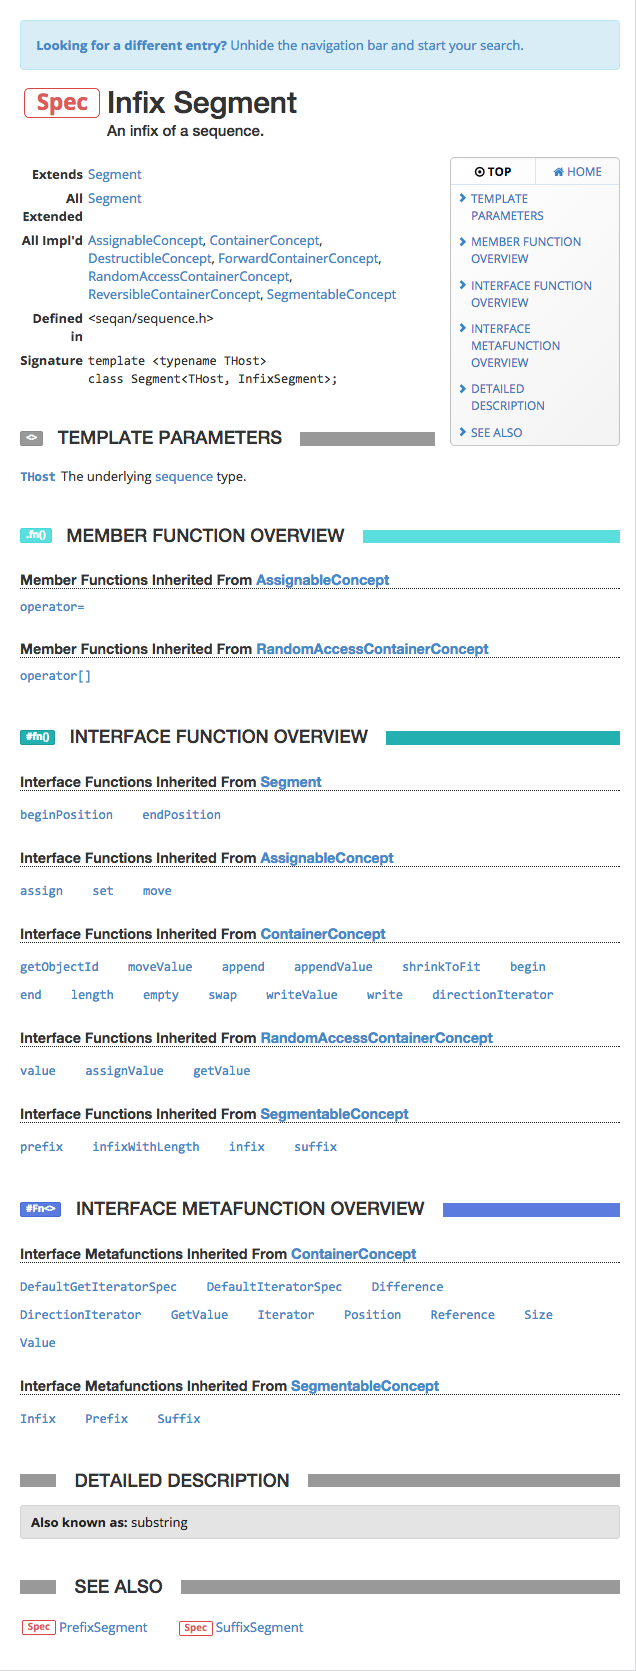
\includegraphics[width=\linewidth]{Figures/dox/infix-new.png}
                \caption[Vergleich Dokumentationseintrag \texttt{Infix} - Neu]{Neu, Stand: 10.04.2015}
                \label{fig:dox-index-compare-new}
        \end{subfigure}%
        \caption{Vergleich Dokumentationseintrag \texttt{Infix}}%
\end{figure}



\subsubsection{Tutorials}
\label{sec:tutorials-improve}

Basierend auf einem etablierten \citep[u.a.][]{Reardon:2008wl,aggarwal2009essentials} Lernphasenmodell \citep{Gagne:1985tx}, den Analyseergebnissen der OOBE-Ressourcen, der Workshops '11 und '12, der PMSB'12-Veranstaltung und einem intensiven Gespräch mit meinen Kollegen am 05.07.2012 --- also knapp ein Jahr nach Beginn der Arbeit --- habe ich die Struktur der Tutorials überarbeitet und Qualitätskriterien formuliert.

Das Ergebnis habe ich in dem Dokument ``Writing Tutorials''\footnote{\url{http://seqan.readthedocs.org/en/master/HowTo/WriteTutorials.html}} zusammengefasst. Es richtet sich an die Autoren von SeqAn-Tutorials und umfasst alle notwendigen Informationen zum Verfassen eines qualitativen Tutorials.

Das eben genannte Dokument ``Writing Tutorials'' verfügt über die folgende Struktur:
\begin{description}
  \item[1. Konventionen] \hfill \\
  Dieser Abschnitt beschreibt, innerhalb eines Tutorials, einzuhaltende Vorgaben.
  \begin{enumerate}
    \item Wiki-Konventionen\\Anforderungen an Wiki-Syntax
    \item Namens-Konventionen\\Anforderungen an Groß- und Kleinschreibung, Benennung des Tutorials, etc.
    \item Design- und Layout-Konventionen\\Anforderung an die Hervorhebung von Schlüsselkonzepten, Verweisen, Programmeingaben und -ausgaben, etc.
  \end{enumerate}
  
  \item[2. Struktur] \hfill \\
  Die Struktur sieht vor, dass ein Tutorial aus einem Meta-Informationen-Block, einer Einführung, inhaltlichen Abschnitten und weiterführenden Links besteht.
  \begin{enumerate}
    \item Meta-Informationen\\Angabe von Lernziel, Schwierigkeitsgrad, voraussichtliche Bearbeitungsdauer und Voraussetzungen mit entsprechenden Links
    \item Einführung\\Tutorial-Inhalt, Relevanz/Wichtigkeit, praktische Anwendungsgebiete und erworbenes Wissen nach Tutorial-Bearbeitung
    \item Abschnitte\\Jeder inhaltliche Abschnitt bespricht einen logischen Lernschritt bestehend aus einem schriftlichen Ausführungen, Beispielen und einer Übungsaufgabe.
    \begin{enumerate}
      \item Einführung\\Abschnittsinhalt, Nennung wichtiger Konzepte, Lernziel
      \item Erklärung\\Eigentlicher Inhalt
      \item Beispiele\\Beispiele, die die Erklärung veranschaulichen und die Umsetzung in SeqAn demonstrieren
      \item Übungsaufgaben\\Wiederholung bzw. Anwendung des erworbenen Wissens
    \end{enumerate}
  \end{enumerate}
  
  \item[3. Didaktik] \hfill \\
  Dieser Abschnitt soll die Autoren von Tutorials für eine benutzerfreundliche, anwender-zentrische Schreibweise sensibilisieren und motivieren.
  \begin{enumerate}
    \item Übungsaufgaben-Typ\\Erklärung der verschiedenen Typen von Übungsaufgaben 
    \item Zeitbedarf\\Schätzung des Zeitbedarfs von Tutorials und Aufgaben
    \item Sprache\\Gebrauch einer einfachen verständlichen Sprache
    \item Mentales Modell\\Einnahme der Leserperspektive
  \end{enumerate}
  
  \item[4. Integration] \hfill \\
  Dieser Abschnitt erläutert technische Fragestellungen wie Orte, an denen ein Tutorial verlinkt werden muss.
  \item[5. Vorlage] \hfill \\
  Dieser Abschnitt stellt eine Vorlage bereit, die über erklärende und zu ersetzende Platzhalter verfügt. So soll sichergestellt werden, dass die Grundstruktur aller neuen Tutorials konsistent bleibt und den qualitativen Anforderungen genügt.
\end{description}

Während manche Tutorials sehr kurz waren, waren andere außerordentlich ausschweifend formuliert. Bei der Bearbeitung Letzterer, gingen wichtige Informationen und Schlüsselkonzepte in der Masse unter. Aus diesem Grund wurden Elemente eingeführt, die explizit den Typ einer Information grafisch mittels einer farbigen Box hervorheben. Es existieren Boxen für wichtige (orange) und optionale (blau) Inhalte (siehe Abbildungen \ref{fig:tutorial-box-important} und \ref{fig:tutorial-box-info}). Darüber hinaus existieren Boxen für Beispiele (grau), Code-Ausschnitte (ebenfalls grau), Programmausgaben (schwarz) und Übungsaufgaben (beige). Außerdem wurden Schlüsselkonzepte fett hervorgehoben und sämtliche genannten Entitäten, wie Funktionen, mit den entsprechenden Dokumentationseinträgen verlinkt.

Die Übungsaufgaben waren vor der Verbesserung von unterschiedlicher Qualität und verfügten über didaktische Schwächen. Diese Probleme sollten u.a. durch die enge Kopplung an einen inhaltlichen Abschnitt gelöst werden. Wichtiger jedoch ist, dass Übungsaufgaben nun von einer der drei folgenden Typen sein müssen: \textit{Review}, \textit{Application}, \textit{Transfer}.

\textit{Review}-Übungen beschränken sich auf die reine Wiederholung von Inhalten und sollen lediglich die Verwendung von SeqAn üben. \textit{Application}-Übungen umfassen Aufgaben, bei denen Variationen vorgenommen werden müssen (z.B. Belegung eines optionalen Parameters). \textit{Transfer}-Übungen sind die anspruchsvollsten und sollen verschiedene Anwendungsmöglichkeiten für das erworbene Wissen aufzeigen.

Eine Forderung an die Übungen ist, dass sie nur in aufsteigender Schwierigkeitsreihenfolge auftauchen dürfen und sich aufeinander beziehen müssen. Beispielsweise darf keine \textit{Review}-Übung auf eine \textit{Application}-Übung folgen. \textbf{Gäbe es tatsächlich für solch einen Fall einen Bedarf, ist das Tutorial wahrscheinlich zu umfassend und muss aufgetrennt werden.} 

\begin{figure}
        \centering
        \begin{subfigure}{0.48\linewidth}
                \raisebox{1.1cm}{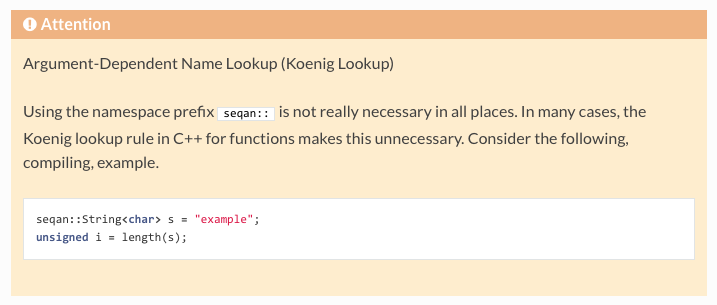
\includegraphics[width=\linewidth]{Figures/tutorial-box-important.png}}
                  \caption{Box für wichtige Inhalte}
                \label{fig:tutorial-box-important}
        \end{subfigure}%
        \hfill%
        \begin{subfigure}{0.48\linewidth}%
                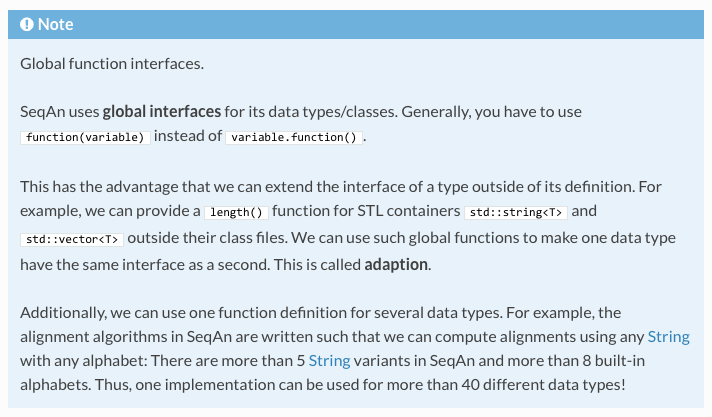
\includegraphics[width=\linewidth]{Figures/tutorial-box-info.png}
                \caption{Box für weiterführende Inhalte}
                \label{fig:tutorial-box-info}
        \end{subfigure}%
        \caption{Boxen zur Auszeichnung von Inhaltstypen}%
\end{figure}

Es wurden mehrere neue Tutorials durch das Auftrennen existierender Tutorials verfasst. Besonders erwähnenswert ist dabei das neue Anfänger-Tutorial ``A First Example''\footnote{\url{http://seqan.readthedocs.org/en/master/Tutorial/FirstStepsInSeqAn.html}}, das eine besonders geringe Einstiegshürde aufweist. Dazu führt es in einfachste Konzepte von SeqAn ein und wird der Beobachtung gerecht, dass viele Anwender einen OOP-Hintergrund haben. 

Die Tutorials wurden sukzessive über eine längere Diskussionsphase hinweg gemeinsam von mir und den jeweiligen Autoren verbessert  (siehe Abbildungen \ref{fig:tutorial-improved}, \ref{fig:tutorial-revisioned} und \ref{fig:tutorial-improved2}). Zum Workshop'12 waren die wichtigsten und zum Workshop'13 alle Tutorials überarbeitet.

\begin{figure}
  \centering
    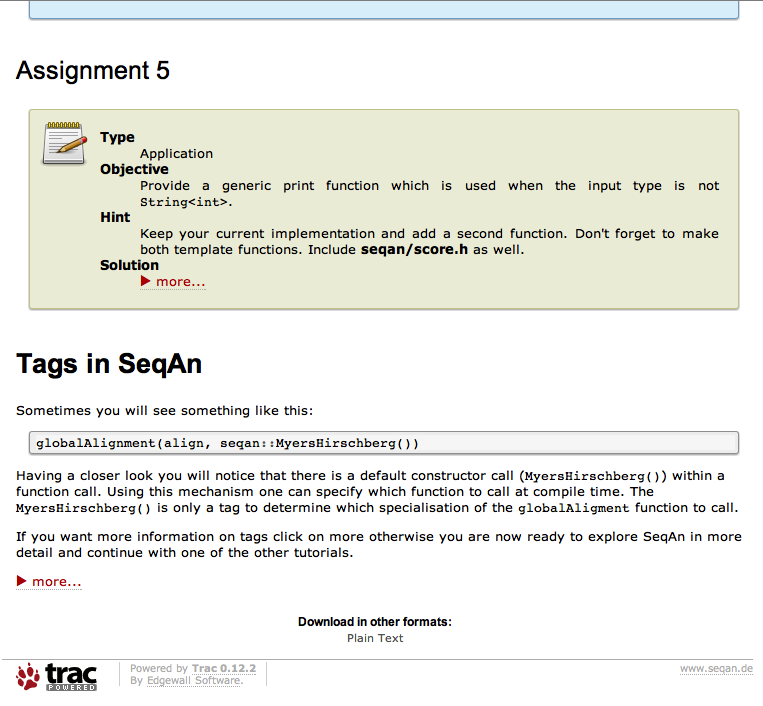
\includegraphics[width=0.57\linewidth]{Figures/tutorial-improved.png}
  \caption{Erste Verbesserung des neuen Anfänger-Tutorials}
  \label{fig:tutorial-improved}
\end{figure}

\begin{figure}
  \centering
    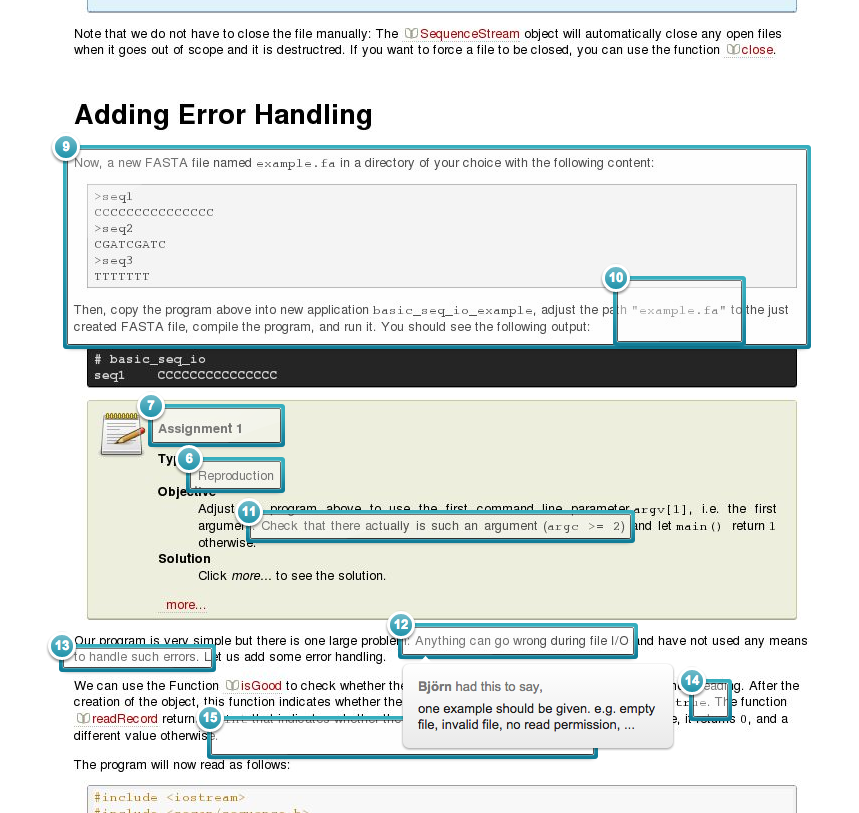
\includegraphics[width=0.65\linewidth]{Figures/tutorial-revisioned.png}
  \caption{Revision der ersten Verbesserung des neuen Anfänger-Tutorials}
  \label{fig:tutorial-revisioned}
\end{figure}

\begin{figure}
  \centering
    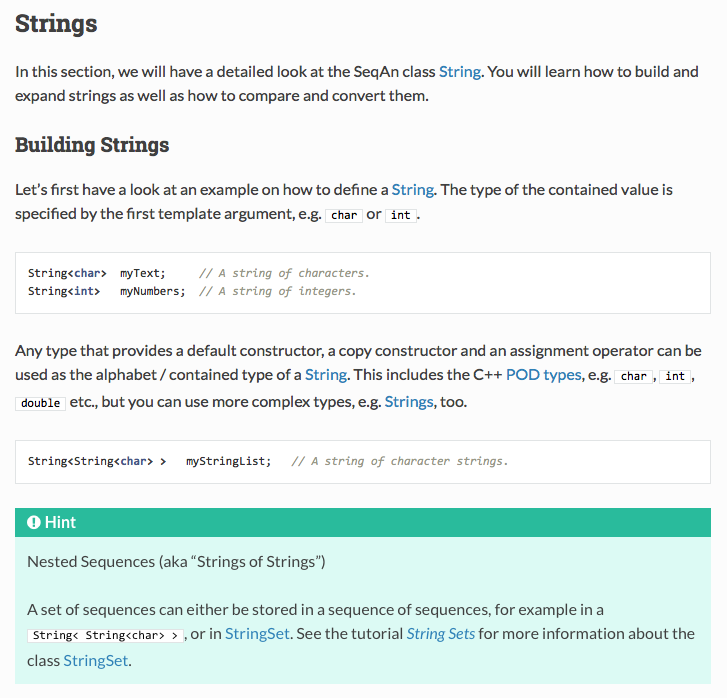
\includegraphics[width=0.55\linewidth]{Figures/tutorial-improved2.png}
  \caption{Zweite Verbesserung des neuen Anfänger-Tutorials}
  \label{fig:tutorial-improved2}
\end{figure}




\subsection{Validierung}
\label{sec:phase1-validierung}

In diesem Abschnitt bespreche ich, wie ich die eben vorgestellten Verbesserungen validiert habe.

\subsubsection{Prozessverbesserungen}

\paragraph{Commit-Nachrichten} Die Vorstellung des neuen Commit-Nachrichtenformats wurde während einer Vorstellung vom SeqAn-Team positiv angenommen. Fast alle darauffolgenden Commit-Nachrichten hielten sich an das Format und vielen deutlicher genauer aus. Als Beispiel habe ich zwei Commit-Nachrichten ausgewählt und jeweils eine inhaltlich passende spätere Commit-Nachricht ermittelt.

\begin{description}
  \item[Beispiel 1] \hfill
  \begin{description}
    \item[Vorher] ``RazerS3: Fixing mate pair modus, deferred compaction.''
    \item[Nachher] ``[FIX] Always adding option -{}-thread-count for RazerS 3, but hiding it in sequential mode.''
  \end{description}
  
  \item[Beispiel 2] \hfill
  \begin{description}
    \item[Vorher] ``Disabling parallel STL in fiona on MinGW.''
    \item[Nachher] ``[API] removed assertions from arg\_parse value accession methods, changed behavior of getValue methods\\
- previously, an assertion ensured that no unset value was requested from the ArgumentParser\\
- now, the method will just not alter the passed reference or will return empty values respectively''
  \end{description}
\end{description}

\paragraph{Umstellung Subversion auf Git}

Die Umstellung auf Git wurde mit dem SeqAn-Team besprochen und eine Einführung wurde gegeben. Alle SeqAn-Entwickler arbeiten zentral und lokal mit Git und können nun lokale Revisionen erstellen, ohne das zentrale Repository zu kompromittieren. Zuvor kam es immer wieder zu Commits, die das Bauen von SeqAn verhinderte.

\paragraph{Code-Reviews}

Die Code-Reviews wurden gut angenommen. Im späteren Verlauf wurde das Prä-Commit-Verfahren auf ein Post-Commit-Verfahren umgestellt. Für Externe gilt weiterhin das Prä-Commit-Verfahren. Ich habe die Codequalität von SeqAn nicht weiter verfolgt, weil ich dieser Verbesserung in Anbetracht meiner eigentlichen \gls{gtm}-Forschung keinen weiteren Raum einräumen wollte. Die gute Annahme seitens der SeqAn-Entwickler deutet aber darauf hin, dass sich die Code-Qualität verbessert hat.


\subsubsection{Argument-Parser}

Sämtliche SeqAn-Anwendungen wurden auf den neuen Argument-Parser umgestellt. Bei der Vorstellung dieses Parsers auf den folgenden Workshops gab es durchweg positives Feedback. Ein Workshop-Teilnehmer sah darin sogar einen Grund, SeqAn allein aus diesem Grund zu verwenden.


\subsubsection{Installation}

Die Installationsanleitungen wurden vollständig überarbeiteten und angeglichenen. Konkrete Hürden bei der Installation von SeqAn (insbesondere unter Windows), wurden auf technischer Seite beseitigt.

Während der Workshops gab es durchweg positives Feedback. Ein Anwender war über die Befragung zu den Installationsanleitungen sogar überrascht und bezeichnete sie als ``vollkommen problemlos''. Ein PMSB'13-Teilnehmer beurteilte die Installationsanleitung als ``idiotensicher''.

Vor der Verbesserung bewertete die Hälfte der Workshop-Teilnehmer die Installation als ``einfach'' oder ``sehr einfach''. Nach der Verbesserung waren es 85\%. Unter den Windows- und Mac-Anwendern kam es zu der deutlichsten Verbesserung.


\subsubsection{Dokumentation}

Die Verbesserung der Dokumentation wird im \sref{sec:improve-dox} und die dazugehörige Validierung im \sref{sec:validierung} besprochen.



\subsubsection{Tutorials}

Die Tutorials sind neben der Dokumentation die wichtigsten Lernressourcen für SeqAn-Anwender. Daher habe ich die Validierung sowohl argumentativ, als auch empirisch vorgenommen. 

\paragraph{Argumentative Validierung}

Bei der Aufgabe des Lernens werden acht sequentielle Phasen durchlaufen \citep{Gagne:1985tx,aggarwal2009essentials}. \cite{Reardon:2008wl} formuliert Instruktionen, die diese Phasen unterstützen und in den SeqAn-Tutorials wie folgt umgesetzt wurden: 

\begin{description}
  \item[1. Motivationsphase] \hfill \\
  Diese Phase wird durch die Tutorial-Metainformationen und -Einführung bedient. Der Anwender kann auf der Grundlage dieser Informationen entscheiden, ob und in welchem Umfang ihn das Tutorial helfen kann. Das gleiche trifft auf die Einführungen der inhaltlichen Abschnitte zu.
  \item[2. Wahrnehmungsphase] \hfill \\
  Durch den Einsatz von typisierten Informationen (z.B. blaue Box für optionale Inhalte) werden wesentliche, von wichtigen und weiterführenden Informationen unterschieden. Durch die unterschiedliche visuelle Darstellung, kann der Anwender schnell diese Informationstypen wahrnehmen.
  \item[3. Akquisitionsphase] \hfill \\
  Diese Phase wird durch Beispiele und Übungsaufgaben des Typs \textit{Review} unterstützt, indem eben wahrgenommenes Wissen verfestigt wird.
  \item[4. Retentionsphase] \hfill \\
  Diese Phase beschreibt die Speicherung von Informationen im Gehirn des Lernenden und kann nicht beeinflusst werden.
  \item[5. Abrufphase] \hfill \\
  Diese Phase wird durch Übungsaufgaben des Typs \textit{Application} unterstützt, indem gespeichertes Wissen, erneut abgerufen und damit verfestigt wird.
  \item[6. Generalisierungsphase] \hfill \\
  Diese Phase wird durch Beispiele und Übungsaufgaben des Typs \textit{Transfer} unterstützt, indem gespeichertes Wissen auf verwandte Aufgabenstellungen angewendet werden muss.
  \item[7. Durchführungsphase] \hfill \\
  Diese Phase wird geringfügig durch die Angabe der voraussichtlichen Bearbeitungsdauer einer jeden Übungsaufgabe unterstützt.
  \item[8. Rückmeldungsphase] \hfill \\
  Diese Phase wird durch die Bereitstellung vollständiger und kompilierbarer Teil- und Gesamtlösungen zu den Übungsaufgaben unterstützt.
\end{description}

Darüber hinaus wird der Anwender durch die Angabe weiterführender Tutorials inspiriert und über weitere Anwendungsgebiete von SeqAn informiert.


\paragraph{Empirische Validierung}

Das neue Einführungs-Tutorial ``A First Example'' wurde sehr positiv von den Workshop'12- und PMSB'12-Teilnehmern angenommen.  80\% der Befragten bewerten dieses Tutorial als überdurchschnittlich (40\%) bzw. außergewöhnlich hilfreich (40\%).

Wurden die Tutorials in ihrer Gesamtheit während des Workshops'11 nur von 24\% als gut oder besser bewertet, waren das nach der Verbesserung zum Workshop'12 ganze 67\%.

Bei der PMSB'12-Befragung gab es durchweg sehr gute Bewertungen, die aber durch die enge Zusammenarbeit mit den SeqAn-Entwicklern verzerrt sein könnte und damit nicht für die Validierung verwendet werden können.
\section{Phase 2: Planung und Durchführung der Datenerhebung}
\label{sec:datenerhebung}\label{sec:phase2}

Da nun die gröbsten Usability-Probleme --- insbesondere bzgl. der Out-Of-Of-Experience --- beseitigt wurden, kann mit der Erforschung der API im engeren Sinne fortgefahren werden. Dazu habe ich für die Analyse, der in diesem Abschnitt vorgestellten erhobenen Daten, die \gls{gtm} verwendet, welche ich bereits im \sref{sec:gtm} vorgestellt habe.

Um eine für die Analysezwecke sinnvolle Datenerhebung zu planen, lohnt sich zunächst der Vergleich mit anderen Studien.



\subsection{Vergleich mit anderen Studien}

In der Arbeit von \cite{deSouza:2004fd} wurde eine nicht-partizipative Feldstudie über einen Zeitraum von 11 Wochen durchgeführt. Dabei wurden Beobachtungen auf nicht weitere definierte Weise festgehalten und semi-strukturierte Interviews durchgeführt.

Bei der fachlich-nahen Arbeit von \cite{Letondal:2006dy} wurden für die Entwicklung eines Anwendung-Entwicklungsumgebung-Hybriden (Ansatz: \textit{Programming In The User Interface}), über mehrere Iterationen hinweg, größtenteils Brainstorming-Sessions und teilweise videoaufgezeichnete Interviews eingesetzt (Details siehe \sref{sec:letondal}).

In der Clarkeschen Forschung \citep[u.a.][]{clarke:2006} werden API-Anwender bei der Lösung gestellter Programmieraufgaben videoaufgezeichnet.

\cite{LaToza:2007fj} beobachtete bei seiner Arbeit ebenfalls Entwickler und zeichnete diese mit Video auf. Des Weiteren wurden die Entwickler instruiert, lautes Denken (engl. \textit{Think Aloud}) anzuwenden. Am außergewöhnlichsten ist jedoch die Instrumentalisierung der \gls{eclipse}-Entwicklungsumgebung, mit deren Hilfe die Autoren diverse Ereignisse innerhalb der Entwicklungsumgebung mitgeschnitten haben. Details zur dieser Arbeit finden sich im \sref{sec:FactFinding}.

Bei der im \sref{sec:concept-maps} näher beschriebenen Concept-Maps-Methode \citep{Tenny:2011jp} werden informelle Gruppendiskussionen mit den API-Entwicklern und -Anwendern geführt und die Ergebnisse an einem Flipchart, für alle zugänglich, festgehalten.

\cite{Grill:2012jm} stellen in ihrer Fallstudie ein Verfahren zur API-Usability-Evaluation vor und nutzen dabei Workshops, die den beim BioStore-Projekt eingesetzten, ähneln. Während dieser Workshops werden API-Anwender bei ihrer Arbeit videoaufgezeichnet und im Anschluss interviewt. Weitere Details finden sich im \sref{sec:grill}.

\cite{Piccioni:2013uq} verwendeten zur Verbesserung einer Persistenz-Bibliothek ebenfalls Videoaufzeichnungen von Problem-lösenden API-Anwendern und anschließenden Interviews (Details siehe \sref{sec:piccioni}).


\subsubsection{Kombination von Methoden}

Die meisten genannten Arbeiten verwenden eine Kombination verschiedener Datenerhebungs- und Analysemethoden. Für die Kombination der, in der klassischen Usability-Evaluation gebräuchlichen Methoden \textit{\acrlong{he}} \citep{Nielsen:1990bw} und \textit{Usability-Test} \citep{Faulkner:2003wn} konnte bereits gezeigt werden, dass diese verschiedenartige Usability-Probleme aufdecken und ideal kombiniert werden können \citep{Fu:2002tp}.

Eine ähnliche Beobachtung konnten \cite{Grill:2012jm} bei der Kombination von semi-strukturierten Interviews und Videoaufzeichnungen machen. Ihre Analyse beider Quellen förderte 168 API-Usablity-Probleme zu Tage, von denen 157 in nur einer der beiden Datenquellen zu finden waren. Sie stellten beispielsweise fest, dass sich Laufzeit-Probleme nicht mit einer \gls{he} auffinden konnten. Außerdem bemerkten sie, dass sie zwar die meisten Probleme mit Hilfe der Interviews fanden, die schwerwiegendsten Probleme jedoch in den Videoaufzeichnungen verborgen waren. Ähnliche Erfahrungen haben auch \cite{Piccioni:2013uq} gemacht.


\subsubsection{Subjektive und objektive Daten}
\label{sec:objektive-vs-subjektive-Daten}

Es gibt in der API-Usability-Forschung einen Trend zur Betonung subjektiver Daten \citep{Rosson:2001uf,Stylos:2008cu,Robillard:2010bh}, dem auch alle mir bekannten API-Evaluationsstudien folgen. Auch wenn Videoaufzeichnungen, technisch betrachtet, objektive Daten darstellen\footnote{\sref{sec:def-usability} befasst sich mit den Klassen der Erhebungs- und Analyseverfahren.}, werden diese meist nur verwendet, um Erklärungslücken bei der Analyse von Interviews zu klären \citep[vgl.][]{Letondal:2006dy,Grill:2012jm,Tenny:2011jp} oder quantitative Betrachtungen vorzunehmen \citep[vgl.][]{Piccioni:2013uq}. Ausschließlich objektive Daten verwenden nach meiner Kenntnis nur zwei API-Evaluationsstudien \citep{deSouza:ek,Watson:2009bm}.

Tatsächlich sind aber beide Datentypen\footnote{Subjektive Verfahren erheben subjektive Meinungen/Ansichten/Darlegungen der Benutzer, wohingegen objektive Verfahren direkt beobachtbare Daten erfassen. Eine ausführlichere Differenzierung beschreiben \cite{Sarodnick:2006vc}.} wichtig:
\begin{description}
  \item[Subjektive Daten] erhalten viele relevante Informationen zu Usability-Problemen \citep{Rosson:2001uf,Stylos:2008cu,Robillard:2010bh,DaqingHou:2005ba}, z.B. in Bezug auf die Anforderungen an das Softwaresystem \citep{eagan2008buzz}. Allerdings besteht die Gefahr, dass Befragte manchen für irrelevant gehaltenen \citep{Daughtry:2009be} oder kritischen Punkt in Interviews \citep[\textit{soziale Erwünschtheit},][]{Hartmann:1991ju} bzw. in Gruppendiskussionen \citep[\textit{Schweigespirale},][]{NoelleNeumann:1989db} nicht äußern. Ebenso so schwer wiegt, dass Probanden auch nur Äußerungen zu Punkten machen können, die ihnen bewusst sind \citep{Ko:2011el}.
  \item[Objektive Daten] In objektiven Daten hingegen manifestieren sich Probleme, die dem Anwender möglicherweise nicht bewusst sind oder nicht korrekt erfragt wurden \citep{Ko:2011el}. Gegebenenfalls kann der Befragte ein Problem nicht verbalisieren, weil er es bereits gelöst hat, bevor er jemals danach gefragt wurde \citep{sunshine2014searching}.
\end{description}

Die Mischung beider Datentypen vereint die jeweiligen Vorteile \citep{Sarodnick:2006vc}. Im Laufe dieser Arbeit habe ich die Erfahrung gemacht, dass die qualitative Analyse objektiver Daten anspruchsvoller ist, als die subjektiver Daten. Objektive Daten enthalten häufig weniger Hinweise darauf, ``wo die Musik spielt''.



\subsubsection{Studienformen}

Die meisten mir bekannten API-Usability relevanten Studien sind Labor- oder Fallstudien. Zu den wenigen partizipativen Feldstudien gehören \cite{Letondal:2006dy} und \cite{Tenny:2011jp}. Die einzige mir bekannte nicht-partizipative Feldstudie ist die von \cite{deSouza:2004fd}.

Langzeitstudien sind rar. Zwei Studien \citep{Tenny:2011jp,deSouza:2004fd} machten Feldbeobachtungen über jeweils elf Wochen hinweg. Die Arbeit von \cite{Letondal:2006dy} fußt auf Datenerhebungen, die über einen Zeitraum von acht Jahren angefertigt wurden.





\subsection{Planung der Datenerhebung}

\subsubsection{Ziele}

Die von mir geplante Datenerhebung, verfolgte zwei primäre Ziele:
\begin{enumerate}
  \item Die Datenerhebung sollte so reichhaltig wie möglich sein, denn die möglichen Zeitpunkte zur Datenerhebung waren begrenzt.
  \item Die Datenerhebung sollte so wenig wie möglich, die Arbeit der SeqAn-API-Anwender beeinflussen, um verallgemeinerbare Aussagen treffen zu können.
\end{enumerate}


\subsubsection{Anforderungen}

Für die Datenerhebung musste ich ein Verfahren entwickeln, das die eben beschriebenen primären Ziele und die daraus folgenden Anforderungen erfüllt:
\begin{itemize}
  \item Die Daten müssen auf den individuellen Arbeitsplätzen der Probanden erhoben werden. Die Probanden sollen also nicht an einer speziell für die Datenerhebung vorbereiteten Arbeitsstation arbeiten, was anderenfalls zu Verfälschungen führt \citep{McKeogh:2004gj}.
  \item Die Datenerhebung muss einfach einzurichten sein, um eine möglichst hohe Bereitschaft zur Datenerhebung auf Seite der Probanden zu erhalten.
  \item Die Datenerhebung muss unauffällig sein und darf den Proband in seiner Arbeit nicht stören.
  \item Die Datenerhebung muss sich für Langzeitbeobachtungen eignen, um auch API-Usability-Probleme zu entdecken, die erst nach längerem Gebrauch einer API auftreten \citep{Stylos:2007jb,Ellis:2007kv} bzw. nicht in einem einzelnen Messpunkt zu beobachten sind \citep{Grill:2012jm,Tenny:2011jp}.
  \item Die Datenerhebung muss datenschutzrechtlichen Anforderungen genügen. Dazu gehört, neben einem einzuholenden Einverständnis, die Möglichkeit, in die erhobenen Daten Einsicht zu nehmen und die Datenerhebung deaktivieren zu können.
  \item Die Datenerhebung muss sowohl subjektive als auch objektive Daten erheben, um einerseits reichhaltige Erkenntnisse zu ermöglichen und andererseits den begrenzten Möglichkeiten zur Datenerhebung Rechnung zu tragen.
  \begin{itemize}
    \item Für meine Forschung setze ich die \gls{gtm} ein, was mögliche weitere Datenerhebungen erfordert (\textit{theoretisches Sampling}). Die besondere Reichhaltigkeit der Daten soll die Wahrscheinlichkeit senken, weitere Daten erheben zu müssen.
    \item Die Reichhaltigkeit der Daten wird durch die Verwendung subjektiver und objektiver Datenerhebungen erreicht (siehe \sref{sec:objektive-vs-subjektive-Daten}).
  \end{itemize}
  \item Die Datenerhebung muss Vertreter der tatsächlichen Anwendergruppe, der zu analysierenden API, umfassen. Nur so lassen sich relevante API-Usability-Probleme erheben \citep{Clarke:2004te,Henning:2007kg}.
\end{itemize}


\subsubsection{Mögliche Datenquellen}

Für die Datenerhebung eigneten sich, die im Rahmen des BioStore-Projekts durchgeführten drei SeqAn-Workshops. Darüber hinaus boten sich die ebenfalls jährlich stattfindenden PMSB-Praktika an. Beide Formate wurde bereits in den Abschnitten \ref{sec:data-sources-workshop} und \ref{sec:data-sources-pmsb} vorgestellt.
 
 
\subsubsection{Konzept}

Um die eben beschrieben Anforderungen, unter Beachtung der möglichen Datenquellen, zu erfüllen, habe ich mich entschieden, eine nicht-partizipative Feldstudie unter Verwendung von zwei Typen von Datenerhebungen durchzuführen --- zwei subjektive und ein objektives Datenerhebungsverfahren. Die Kombination unterschiedlicher Erhebungsverfahren hat sich bewährt \cite[vgl.][]{LaToza:2007fj,deSouza:2004fd,Letondal:2006dy,Grill:2012jm,Piccioni:2013uq}.

Als subjektive Datenerhebungsverfahren sollten ein \textit{Cognitive-Dimensions-Fragebogen} und eine \textit{Gruppendiskussion} zum Einsatz kommen. Für das objektive Verfahren sollten Aufzeichnungen der Fortschritte dienen, die SeqAn-Anwender bei der Entwicklung von, auf SeqAn-basierenden Programmen entwickeln. Letzteres bezeichne ich als \textit{Programmierfortschritte}-Erhebung. Alle drei Verfahren werden in folgenden Abschnitten vollständig beschrieben.

In der ersten Analysephase habe ich die Anwenderschaft von SeqAn charakterisiert (siehe \sref{sec:results-users}). Zu dieser gehören berufstätige, nationale und internationale Wissenschaftler aus den Bereichen Informatik, Bioinformatik und der Physik. Ich betrachte diese Personen als geeignete Probanden für meine Forschung. Der Studentenanteil stellt keine Probleme dar, da er einen beachtlichen Teil zur bioinformatischen Arbeit beiträgt \citep{Letondal:2006dy} und damit mindestens zur zukünftigen Anwendergruppe gerechnet werden kann.

















\subsection{Gruppendiskussion}
\label{sec:gruppendiskussion}

Als erste Datenquelle habe ich eine Gruppendiskussion nach \cite{mayring2002einfhrung} konzeptioniert und durchgeführt. Die Gruppendiskussion ist ein Verfahren, das von keiner mir bekannten Studie verwendet wurde. Lediglich bei \cite{Tenny:2011jp} werden informelle Gespräche in der Gruppe geführt. 

Interviews wurden zwar in einigen Studien angewandt \citep[vgl.][]{deSouza:2004fd,Letondal:2006dy,Grill:2012jm,Piccioni:2013uq}, haben jedoch gegenüber der Gruppendiskussion Nachteile, ``denn die Erfahrungen zeigen, dass in gut geführten Gruppendiskussionen Rationalisierungen, psychische Sperren durchbrochen werden können und die Beteiligten dann die Einstellungen offen legen, die auch im Alltag ihr Denken, Fühlen und Handeln bestimmen.'' \citep[][S. 77]{mayring2002einfhrung}

Als subjektive Datenquelle hatte die Gruppendiskussion in meiner Arbeit den Vorteil, mich für die von den Anwendern empfundenen Usability-Probleme in SeqAn sensibler zu machen --- ohne ihnen im Vorhinein eine wegweisende Wichtigkeit zu geben, wie das bei der Usability-Evaluation nach \cite{Grill:2012jm} der Fall ist.


\subsubsection{Planung und Vorbereitung}

Nach \cite{mayring2002einfhrung} besteht eine Gruppendiskussion aus den folgenden vier Phasen:

\begin{description}
  \item[1. Darbietung Grundreiz] \hfill \\ Diese Phase dient dazu, das Thema der Diskussion knapp vorzustellen.
  \item[2. Freie Diskussion] \hfill \\ In dieser Phase findet die eigentliche Diskussion statt. 
  \item[3. Weitere Reizargumente] \hfill \\ Kommt die Diskussion ins Stocken, können weitere Reizargumente vorgestellt werden.
  \item[4. Metadiskussion] \hfill \\ Diese Phase dient der Diskussion über die geführte Diskussion und soll eine letzte Reflektion anregen.
\end{description}

Die Analyse aus Phase 1 (siehe \sref{sec:phase1}) hat gezeigt, dass SeqAns größtes Usability-Problem im Bereich des Programmierparadigmas Templatemetaprogrammierung verortet ist. Darum habe ich dieses Thema als Grundreiz gewählt.

Die Gruppendiskussion sollte am letzten Tag des Workshop'12 stattfinden. Für die Behebung grober Usability-Probleme habe ich bei diesem Workshop ebenfalls, die bereits im \sref{sec:feedback} vorgestellten Feedback-Zettel eingesetzt. Die auf den Zetteln geäußerten Punkte und die Ergebnisse meiner \glslink{he}{Heuristischen Evaluation} dienten mir als Reizargument.

Die Reizargumente (die Quelle steht in Klammern) lauten konkret:
\begin{itemize}
  \item STL-Konformität (Feedback)
  \item Operatorenüberladungen (Feedback, HE)
  \item Lesbarkeit von Compilerfehlern (Feedback, HE)
  \item Online-Dokumentation (Feedback, HE)
  \item Konkrete API-Probleme, insbesondere \texttt{Shape}, \texttt{Hash} und \textit{Index} (Feedback)
  \item \texttt{Iterators}, \texttt{StringSet} (Feedback, HE)
  \item Namenskonventionen (Feedback, HE)
  \item Rückmeldung von Lesefehlern (Feedback, HE)
\end{itemize}

Für die Diskussion habe ich 30 Minuten vorgesehen --- mit der Verlängerungsoption um weitere 30 Minuten. Die Diskussion sollte audioaufgezeichnet werden. Für eine maximale Ausdrucksfreiheit, sollte ein Whiteboard zu Verfügung gestellt werden.

Aus dem SeqAn-Team habe ich ein Mitglied für die technische\footnote{Der technische Beobachter hält Mimik und Gestik von Diskussionsteilnehmern schriftlich fest.} und drei Mitglieder für die fachliche Beobachtung\footnote{Die fachlichen Beobachter halten inhaltlich relevante Äußerungen schriftlich fest.} ausgewählt \citep[Details siehe][]{mayring2002einfhrung}. Alle Beobachter wurden von mir vor der Gruppendiskussion schriftlich und mündlich eingewiesen.

Die übrigen Team-Mitglieder habe ich der Diskussion, wegen meiner negativen Erfahrungen bei der Feedback-Runde des Workshops'11 (vgl. \sref{sec:schwierigkeiten}), ausgeschlossen. Dies habe ich getan, um das Phänomen des \textit{technischen Wegargumentierens} zu vermeiden. Damit sollte verhindert werden, dass die Hemmschwelle zur freien Meinungsäußerung angehoben wird, der Diskussionsverlauf durch anderen SeqAn-Entwickler beeinflusst wird oder gar ``Revierkämpfe'' ausgefochten werden.

Ich war mir bewusst, dass der Ausschluss wichtiger SeqAn-Entwickler das Verständnis detailliert vorgetragener, technischer Kritik erschweren kann. Darum sollten sich die Beobachter in der zweiten Hälfte der Gruppendiskussion selbst einbringen dürfen. Dabei wurden die, nun als SeqAn-Experten dienenden Beobachter darum gebeten, eine gewaltfreie Sprache \citep[vgl. \textit{klientenzentrierte Gesprächsführung} nach Carl R. Rogers in][]{Wingchen:2014uk} zu verwenden und unbedingt Äußerungen wie ``Dummer Vorschlag!'', ``Geht nicht, weil...'' oder ``Wozu?!'' zu vermeiden.


\subsubsection{Durchführung und Fazit}

Die Gruppendiskussion fand am 06.09.2012 --- also am letzten Tag des Workshop'12 -- statt. Die Durchführung entsprach der Planung und verlief sehr gut. Der Diskussionsbedarf war so groß, dass die volle Zeit von einer Stunde ausgeschöpft wurde und aus terminlichen Gründen abgebrochen werden musste.

Die von \cite{mayring2002einfhrung} beschriebene erleichterte Offenlegung von, und Reflektion über tatsächliche Alltagsärgernisse, konnte ich klar feststellen. Bei der Darlegung des Grundreizes \textit{Templatemetaprogrammierung} und der Reizargumente \textit{Namenskonventionen} und \textit{Rückmeldung von Lesefehlern} entwickelte sich eine ausgeprägte Dynamik. Das führe ich auf die gute inhaltliche Vorbereitung und auf den Ausschluss der meisten SeqAn-Entwickler zurück. Dennoch war vereinzelt, gegen Ende der Diskussion \textit{technisches Wegargumentieren} zu beobachten.

Für die Metadiskussion verblieben aus Zeitgründen leider nur wenige Minuten. Die Gruppendiskussion wurde von zwei Dritteln der Teilnehmer als sehr positiv bewertet und als notwendig erachtet. Einzelne Teilnehmer sagten, dass diese Diskussion eine einmalige Erfahrung für sie war.

Die pseudonomysierte Transkript befindet sich im \aref{app:gruppendiskussion}. Die Gruppendiskussion wurde mit Hilfe der \gls{gtm} analysiert. Die Ergebnisse werden in den Abschnitten \ref{sec:phase4} und \ref{sec:Ergebnisse} vorgestellt.






\subsection{Cognitive-Dimensions-Fragebogen}
\label{sec:cdf-usage}

Das \gls{cdf} ist ein Diskussionswerkzeug für die Bewertung der Benutzerfreundlichkeit von so genannten \textit{Notationen} (siehe \sref{sec:cdf}). Um die, im Framework formulierten, \glslink{cd}{kognitiven Dimensionen (CD)} zu ermitteln und damit Einsichten in den zu untersuchenden Gegenstand zu erhalten, gibt es die Möglichkeit, einen generischen Fragebogen \citep{161956} einzusetzen (siehe \sref{sec:cdf-questionnaire}). Alternativ hat \cite{Kadoda:2000vj} selbst einen Fragebogen entwickelt, der allerdings nur relevant erschienende CDs umfasst und selbst nicht veröffentlicht wurde.

Für die Evaluation eignet sich allerdings auch nicht der generische Fragebogen. Seine größte Schwäche ist seine Generizität, die von den Autoren als seine größte Stärke herausgestellt wird. Tatsächlich stellten aber Selbige im Rahmen ihrer Pilotstudie fest, dass Anwender Probleme beim Verständnis der generischen Fragen hatten.


\subsubsection{Planung und Vorbereitung}

Um das Problem der Generizität zu lösen, habe ich selbst einen Fragebogen entwickelt, der nicht mehr allgemein von einer ``Notation'', sondern konkret von ``SeqAn'' spricht. Das heißt, ich habe den generischen Fragebogen auf SeqAn instanziiert/spezialisiert.

Genauer gesagt habe ich unter anderem folgende Anpassungen vorgenommen:
\begin{itemize}
  \item Ersetzung produktrelevanter Begriffe durch ``SeqAn'' bzw. ``API''
  \item Entfernung des zweiten Abschnitts\\Dieser Abschnitt umfasst, bei Schriftgröße 10, eine ganze A4-Seite und dient nur dazu, die generischen Termini \textit{Product}, \textit{Notation}, \textit{Helper Device}, \textit{Redefinition Device} und \textit{Sub-Device} so zu erklären, dass der Befragte den Fragebogen auf den Sachgegenstand beziehen kann.
  \item Umformulierung der generischen Aktivitäten zu API-relevanten Aktivitäten, wie ``Implementieren von Code'' oder ``Umstrukturieren von Code''
  \item Verwendung einer Mischung aus den originären CDs und denen von \cite{Anonymous:9HSMlhmF}
  \item Formulierung von Fragen für die neuen 12 CDs
\end{itemize}

Im \sref{sec:api-cds} beschreibe ich den Wert der Arbeit von \cite{Anonymous:9HSMlhmF}, zeige aber auch Unzulänglichkeiten auf. So wurden beispielsweise die originären CDs \textit{Fehleranfälligkeit} und \textit{Vorläufigkeit} entfernt, ohne dass diese durch die anderen CDs abgedeckt wären. Auf der Grundlage der 14 CDs von \cite{161956} und den 12 CDs von \cite{Anonymous:9HSMlhmF} habe ich eigene 12 CDs entwickelt, die auch die beiden entfernten CDs umfassen.

Der Fragebogen wurde als Online-Formular entwickelt. \fref{fig:cd-fragebogen-de-part} zeigt einen Ausschnitt. Alle von mir verwendeten \glslink{cd}{kognitiven Dimensionen}, die dazugehörigen Fragen und der vollständige Fragebogen befinden sich im \aref{app:cd-fragebogen}.

\begin{figure}
  \centering
    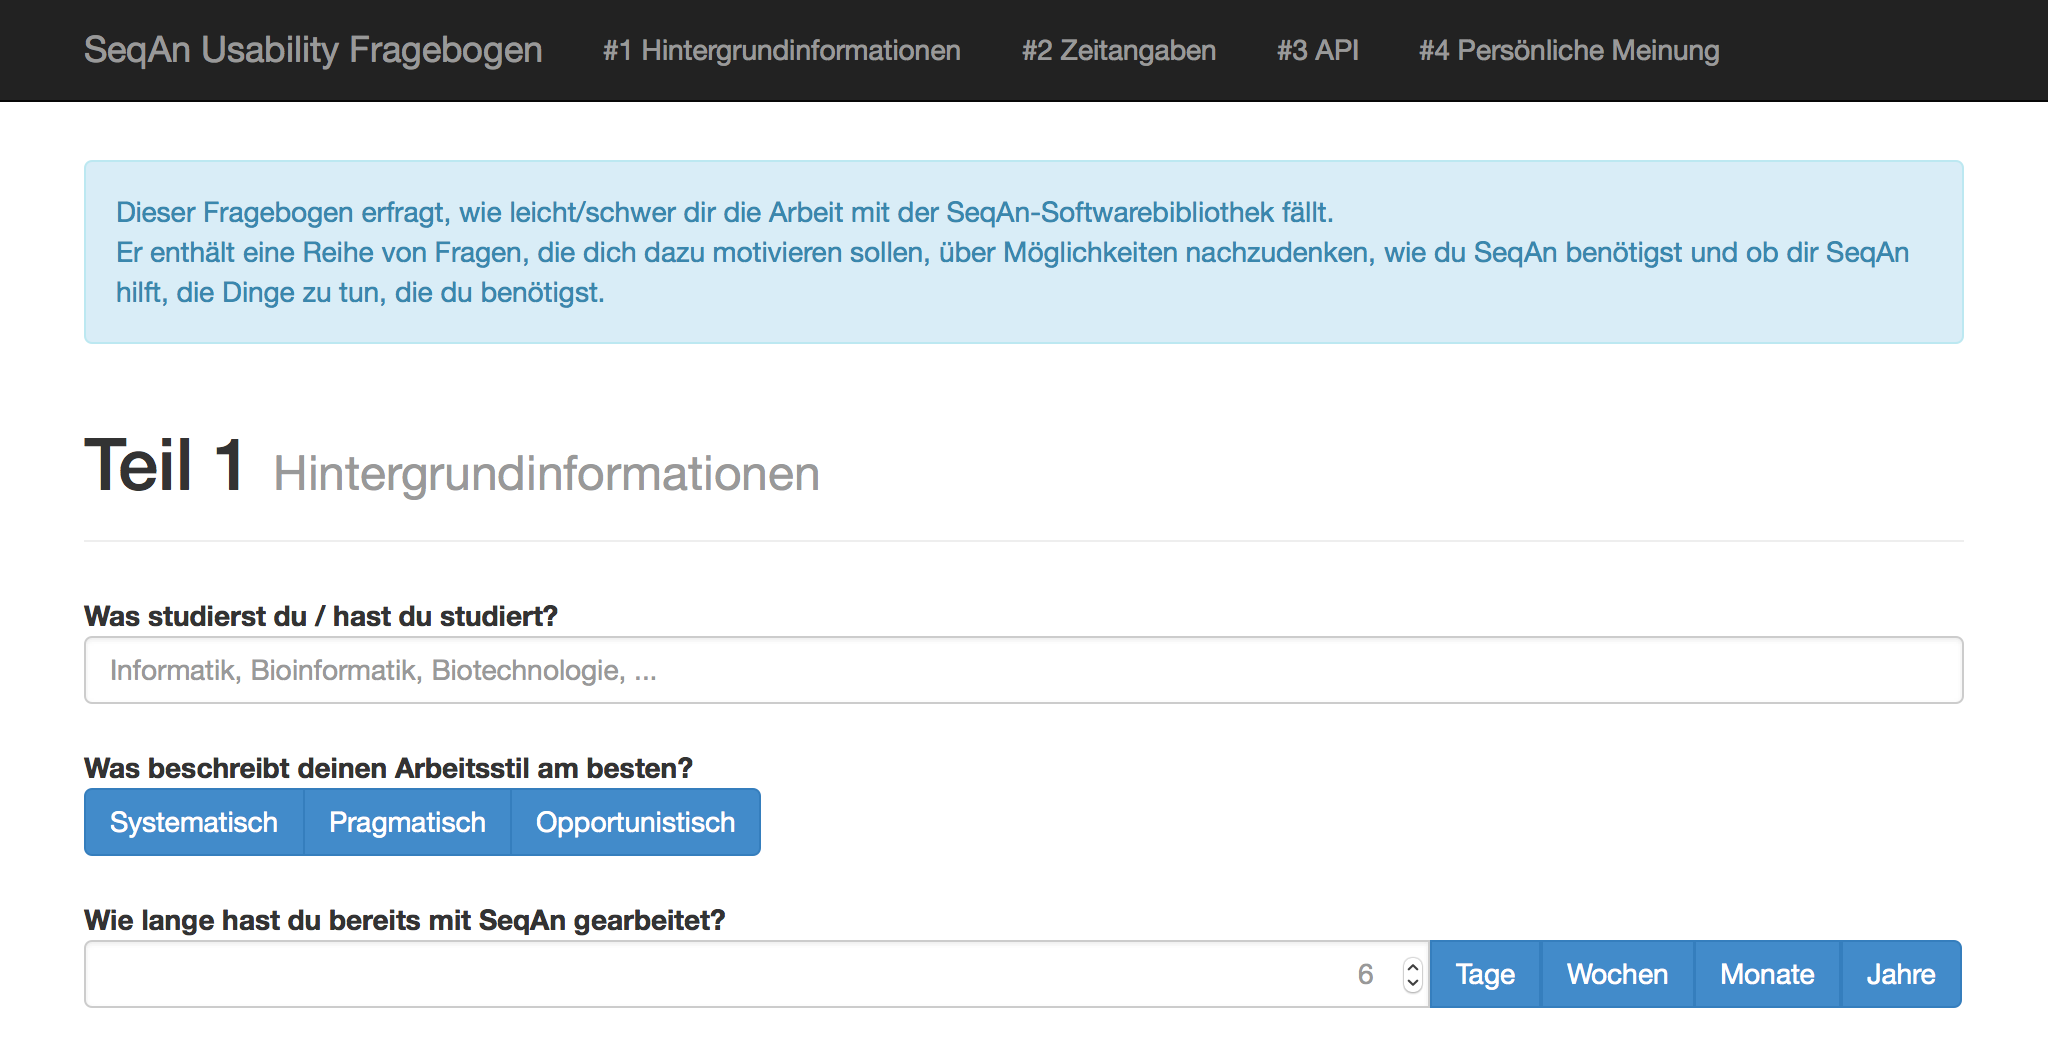
\includegraphics[width=1.0\linewidth]{Figures/cd-fragebogen-de-part.png}
    \caption{Ausschnitt aus dem deutschsprachigen Cognitive-Dimensions-Fragebogen}
    \label{fig:cd-fragebogen-de-part}
\end{figure}

Gemeinsam mit meinen Arbeitskollegen und den Autoren des Cognitive Dimension Frameworks Alan Blackwell und Thomas Green habe ich den Fragebogen mehrfach revisioniert. In einer Mail vom 21.03.2013 hat Alan Blackwell den Fragebogen abschließend mit ``looks nice'' beurteilt.


\subsubsection{Durchführung und Fazit}

Die Befragung mit Hilfe des Fragebogens fand im Rahmen des Workshops'13 statt.

Der von mir investierte Aufwand zeigt, dass es vollkommen unverhältnismäßig gewesen wäre, jedem Befragten diese Transfer-Leistung aufzubürden. An dieser Stelle kann man auch die Argumentation von \cite{Henning:2007kg,Ellis:2007kv} anwenden: Fragebögen werden von viel mehr Menschen ausgefüllt als entworfen. Es ist also ökonomisch absolut sinnvoll, die Instanziierung/Spezialisierung eines Fragebogens durch deren Autoren durchführen zu lassen.

\label{sec:cdf-usage-difficulties}
Insgesamt betrachtet, bleibt ein Cognitive-Dimensions-Fragebogen anspruchsvoll. Bei drei Probanden kam es bei jeweils einer Frage zu Missverständnissen\footnote{Beispiel: In einer Frage zu der CD \textit{Hard Mental Operations} wurde die Formulierung ``when combining things'' verwendet. Die Frage zielte auf die Verarbeitung verschiedener Informationen im Arbeitsgedächtnis abgezielt. Ein Proband jedoch bezog sie auf die Verknüpfung zwischen Funktion und dessen Dokumentationseintrag (siehe \url{apiua://survey/cd/2013-09-18T17:41:31.929+02:00/hardMentalOperations}).}. Eine Reihe von Fragen wurden von manchen Probanden nicht beantwortet. Die Begeisterung für den Fragebogen war geteilt. Ein Proband bezeichnete ihn als ``anstrengend''\citepurl{apiua://survey/cd/2013-09-18T17-45-54.88891500+0200/questionnaire}. Andere Probanden hingegen bewerteten den Fragebogen als ``Super''\citepurl{apiua://survey/cd/2013-09-18T17-46-05.89001200+0200/questionnaire} oder ``Klasse!''\citepurl{apiua://survey/cd/2013-09-18T17-50-13.42530400+0200/questionnaire}.

Die aufgefüllten Fragebögen wurden mit Hilfe der \gls{gtm} analysiert. Die Ergebnisse werden in den Abschnitten \ref{sec:phase4} und \ref{sec:Ergebnisse} vorgestellt.




\subsection{Programmierfortschritte-Erhebung}
\label{sec:programmierfortschritte}

Bei dieser Datenerhebungmethode handelt es sich um eine, die ich selbst entwickelt habe und in keiner mir bekannten Studie angewendet wurde. Sie besteht in der Erhebung von Daten, die den Entwicklungsprozess von Anwendungen, die von SeqAn-Anwendern entwickelt werden, nachvollziehbar machen sollen.


\subsubsection{Planung und Vorbereitung}

Um die Programmierfortschritte der verschiedenen SeqAn-Anwender dokumentieren zu können, benötigte ich die erstellten und veränderten Quellcode-Dateien, die bei der Programmentwicklung anfallen. Diese sollten bei jedem Versuch, den eigenen Programmcode zu kompilieren, erhoben werden, da davon auszugehen ist, dass dann ein irgendwie gearteter Arbeitsschritt abgeschlossen ist.

Um den Verständnisprozess des Anwenders besser verstehen zu können, interessierten mich auch die Zugriffe auf die Online-Dokumentation. Es war abzusehen, dass zwischen zwei Kompilierversuchen mehrere Minuten vergehen können. Die Zugriffe auf die Dokumentation sollten helfen, diese Lücken besser zu verstehen --- beispielsweise, ob ein SeqAn-Anwender gerade einen Dokumentationseintrag liest. Des Weiteren konnte ich so die Online-Dokumentation im Gebrauch durch den Anwender untersuchen. Dies zu können ist essentiell, weil die Dokumentation selbst Bestandteil der API im weiteren Sinne ist und eine wichtige Ressource zum Erlernen einer API darstellt \citep{Robillard:2009cs,Robillard:2010bh}.

Zu guter Letzt interessierten mich Daten zur Arbeitsumgebung, wie der verwendeten Entwicklungsumgebung.

Für die Datenerhebung selbst habe ich eine technische Lösung geplant und unter Verwendung einer Client-Server-Architektur implementiert.


\paragraph{Client}
\label{sec:apiua-client}

Die Datenerhebung auf den individuellen Arbeitsplätzen sollte so transparent laufen und einzurichten sein, wie möglich. 

SeqAn verwendet \textit{CMake}\footnote{\url{http://www.cmake.org}} als plattformübergreifendes Build-System. Als SeqAn-Anwender muss man bei der Installation, zunächst SeqAn herunterladen und dann, mit Hilfe von CMake, die notwendigen Projektdateien für die eigene Entwicklungsumgebung erstellen. Anschließend kann man mit SeqAn in der Entwicklungsumgebung seiner Wahl arbeiten.

Für die Datenerhebung habe ich die CMake-Dateien von SeqAn --- und damit den Build-Prozess --- so verändert, dass nach jedem Kompilierversuch ein Script ausgeführt wird, das Änderungen im SeqAn-Verzeichnis erkennt. Die betroffenen Dateien werden bei diesem Prozess in ein ZIP-Archiv gepackt und auf einen Datenerhebungsserver asynchon hochgeladen.

Der von mir entwickelte Datenerhebungsclient ist auf GitHub gehostet\footnote{\url{https://github.com/bkahlert/api-usability-analyzer-client-python}}.

\paragraph{Server}
\label{sec:apiua-server}

Die Server-Komponente dient der Sammlung der, von den Clients hochgeladenen Daten. Außerdem stellt er ein selbst entwickeltes JavaScript bereit, das in jede beliebige Webseite integriert werden kann und auf minutiöse Weise eine große Spannbreite an Ereignissen auf den instrumentierten Webseiten mitschneidet.

Die Server-Komponente habe ich in Form einer Java EE Web-Anwendung implementiert und auf GitHub bereitgestellt\footnote{\url{https://github.com/bkahlert/api-usability-analyzer-server-java-ee}}.

Das JavaScript zur Webseiten-Überwachung ist Bestandteil des Servers und verwendet ein interessantes Verfahren zur Umgehung der so genannten \textit{Same-Origin-Policy} (siehe \hyperref[subsec:same-origin-policy]{grauer Kasten}).

\begin{furtherreading}[frametitle={Website-Überwachung im Detail}]
\label{subsec:same-origin-policy}
Um eine Webseite (z.B. \texttt{client.com}) mit Hilfe des Datenerhebungsservers zu überwachen, muss zunächst eine JavaScript-Datei in die zu überwachende Seite eingebunden werden. Dies geschieht mit folgendem HTML-Code:
\begin{minted}[linenos=false, firstnumber=1, autogobble=false]{html}
<script src="https://srv.tld/SUAsrv/static/js/SUAclt.js"></script>
\end{minted}

Der kanonische Weg zur Übermittlung von Ereignissen, wie dem Laden oder Verlassen einer Seite, wäre die Absetzung einer Ajax-Anfrage\footnote{\url{http://www.w3.org/2007/06/mobile-ajax/}}. Dabei handelt es sich inhaltlich nicht um eine Anfrage sondern um eine Übermittlung von Daten (hier: Nutzeraktivitäten).

Ajax-Anfragen unterliegen jedoch der Same-Origin-Policy\footnote{\url{http://www.ibm.com/developerworks/web/library/wa-crossdomaincomm/index.html?ca=drs-\#N1019B}}, die den Zweck hat, Datendiebstahl und andere Angriffsformen zu verhindern. Die Übermittlung an einzelne Domains (hier: \texttt{srv.tld}) kann zwar erlaubt werden, wird allerdings nicht von älteren Browsern unterstützt\footnote{\url{https://developer.mozilla.org/en-US/docs/Web/HTTP/Access_control_CORS}}.

Um die Datenübermittlung auch bei älteren Browsern zu unterstützen, werden keine Ajax-Anfragen, sondern \textit{JSONP}-Anfragen\footnote{\url{http://bob.ippoli.to/archives/2005/12/05/remote-json-jsonp/}} abgeschickt. Technisch gesehen, wird dabei ein Script mit Hilfe des \texttt{<script>}-Tags in das \textit{Document Object Model} der überwachten Seite eingefügt, das ein Script lädt und dabei Parameter übergibt. Dabei dienen die belegten Parameter der Datenübermittlung. Das zurückgegebene Script enthält optional Rückgabedaten, die in diesem Fall aber irrelevant sind. Diese Art der Datenübermittlung unterliegt nicht der Same-Origin-Policy und erlaubt so die Übertragung der Nutzeraktivitäten.
\end{furtherreading}


\paragraph{Datenquelle: Arbeitsumgebung}

Für die Analyse der Programmierfortschritte kann es hilfreich sein, Daten zur Arbeitsumgebung des API-Anwenders zu kennen.
  
Dazu übermittelt der, weiter oben beschriebene Client bei der ersten Einrichtung der Entwicklungsumgebung Daten zum Betriebssystem und zur Entwicklungsumgebung an den Server. \lref{lst:apiua-data-demografisch} zeigt Inhalt und Struktur der übermittelten, JSON-formatierten Daten.

\begin{center}
\begin{minted}[linenos=false, firstnumber=1, autogobble=false]{json}
{
  "machine": {
    "machine": "x86_64",
    "processor": "i386",
    "architecture": "64bit"
  },
  "devenv": {
    "CMAKE_CXX_COMPILER": "/usr/bin/g++",
    "CMAKE_GENERATOR": "Xcode"
    },
  "os": {
    "platform": "Darwin-11.1.0-64bit"
    }
}
\end{minted}
\captionof{listing}{Beispiel: Daten zur Arbeitsumgebung}
\label{lst:apiua-data-demografisch}
\end{center}


\paragraph{Datenquelle: Quelldateien}

Bei jedem Kompilierversuch werden alle geänderten Dateien im SeqAn-Arbeitsverzeichnis vom Client in Form eines ZIP-Archivs an den Server übermittelt. Das Senden findet asynchron statt, um den Kompilierprozess nicht zu verlangsamen.

Das ZIP-Archiv erhält dabei einen Namen, der folgende Informationen enthält:
\begin{description}
  \item[ID] des Probanden. Diese ID identifiziert jeden Probanden eindeutig.
  \item[Hash-Wert] des SeqAn-Arbeitsverzeichnis-Pfades. Existieren mehrere SeqAn-Installationen auf einem Rechner, können diese so unterschieden werden.
  \item[Zeitpunkt] des Kompilierversuchs. Für den Zeitpunkt wird eine abgewandelte Form des, in der ISO 8601\footnote{\url{http://www.iso.org/iso/home/standards/iso8601.htm}} festgelegten Formats zur Darstellung von Datum und Zeit, verwendet. Diese Anpassung war notwendig, da beispielsweise der Doppelpunkt auf den meisten Dateisystemformaten nicht erlaubt ist.
\end{description}

Ein beispielhafter Name für ein übermitteltes ZIP-Archiv lautet: \texttt{6ndbc4zuiueuaiyv\_b9dc\_2013-04-09T10-31-07.379654+0200.diff.zip}.


\paragraph{Datenquelle: Onlinedokumentation}

Um die Verwendung einer Webseite durch einen Anwender nachvollziehen zu können, reicht es nicht, das Laden der entsprechenden Seite zu protokollieren.

Stattdessen müssen weitaus differenziertere Ereignisse protokolliert werden:
\begin{description}
  \item[READY] Die Seite wurde vollständig geladen.
  \item[UNLOAD] Die Seite wurde geschlossen.
  \item[FOCUS] Die Seite (bzw. der Browser-Tab) hat den Fokus erhalten.
  \item[BLUR] Die Seite (bzw. der Browser-Tab) hat den Fokus verloren.
  \item[RESIZE] Die Größe der Anzeigefläche wurde verändert. Üblicherweise passiert dies durch die Veränderung der Fenstergröße. Aber auch eingeblendete Browser-Menüs können dieses Ereignis provozieren.
  \item[SCROLL] Der Anwender hat innerhalb der Seite gescrollt.
  \item[TYPING] Der Anwender hat eine Text-Eingabe vorgenommen.
  \item[LINK] Der Anwender hat auf einen Link geklickt.
\end{description}

Bei jedem Ereignis werden, durch das vom Datenerhebungsserver ausgelieferte Script, eine Reihe von Daten asynchron übertragen: Zeitstempel, Ereignistyp, \acrshort{uri} der Seite, IP, Proxy-IP, Scrollposition und Größe der Anzeigefläche. Darüber hinaus werden Ereignis-abhängige Daten übermittelt, wie beim \textit{TYPING}-Ereignis die eigentliche Eingabe und der Name des Eingabefeldes.

Im \sref{sec:doclog} auf Seite \pageref{sec:doclog} stelle ich das Datenformat genauer vor. Dort befindet sich auch ein Auszug aus den so erfassten Daten (siehe \lref{lst:doclog-file}).



\paragraph{Identifikation und Datenschutz}
\label{sec:id}

Eben habe ich drei Datenquellen beschrieben, die in ihrer Gesamtheit die Programmierfortschritte eines Anwenders protokollieren. Allerdings stellt sich die Frage, wie die Datenquellen den Probanden zugeordnet werden können.

Die Identifikation eines Anwenders wird wie folgt realisiert:
\begin{itemize}
  \item Der Anwender muss die Datei \texttt{.APIUA} in seinem Benutzerverzeichnis anlegen. Damit weiß SeqAns Build-Prozess, dass eine Datenerhebung erlaubt ist. Darüber hinaus muss der Proband eine \textit{Einverständniserklärung zur Datenerhebung} (siehe \aref{app:declaration-of-consent}) unterschrieben haben, die ihn über den Umfang der Datenerhebung aufklärt.
  \item Bei der Einrichtung der SeqAn-Installation erfolgt durch den Anwender ein \textit{CMake}-Aufruf. Der von mir veränderte SeqAn-Build-Prozess prüft das Vorhandensein der \texttt{.APIUA}-Datei und aktiviert ggf. die Datenerhebung.
  \item Es wird eine zufällige 16-stellige alphanumerische ID erzeugt und in der Datei \texttt{.APIUA-ID} abgelegt --- ist sie bereits vorhanden, wird die darin enthaltene ID wiederverwendet.
  \item Der Standard-Browser wird geöffnet und eine spezielle Seite auf dem Datenerhebungsserver aufgerufen. Dabei wird die generierte ID an den Server übermittelt. Dem Anwender erscheint eine Seite, die sich für die Bereitschaft zur Datenübermittlung bedankt, die ID des Anwenders zeigt und das Verfahren zur Datenübermittlung erklärt (siehe \fref{fig:apiua-activation}).
  \item Die, auf dem Client erhobenen Arbeitsumgebungsdaten und Quelldateien enthalten in ihrem Dateinamen diese ID.
  \item Zur Identifikation des Browsers wird ein sogenannter \textit{Browser-Fingerprint} verwendet. Dabei wird ein Hash über diverse Datenpunkte (Browser, Betriebssystem, Zeitzone, etc.) berechnet.
  \item Durch den Aufruf der Bestätigungsseite erfährt der Server sowohl die übermittelte ID als auch den jeweils mit übermittelten Browser-Fingerprint. Dieses Tupel wird von dem Server gespeichert.
  \item Zukünftige Aufrufe von beobachteten Seiten übermitteln nun Nutzeraktivitäten an den Server. Mit Hilfe des Browser-Fingerprints, können diese Datenübermittlungen der ID des Anwenders zugeordnet werden.
  \item Der Browser-Fingerprint ist nicht dauerhaft stabil und kann sich, beispielsweise durch die Installation von Updates, verändern. Ich habe ein Verfahren entwickelt, dass überaus stabil ist und selbst das Löschen von Cookies überlebt. Mehr Details befinden sich im \hyperref[subsec:browser-fingerprint]{grauen Kasten}.
  \item Die im \sref{sec:feedback} beschriebenen Feedback-Zettel aus Phase 1, konnten von den Befragten ebenfalls mit ihrer ID versehen werden, um ein ganzheitliches Bild der Probanden zu erhalten (siehe \fref{fig:survey-id}).
\end{itemize}

\begin{figure}
  \centering
    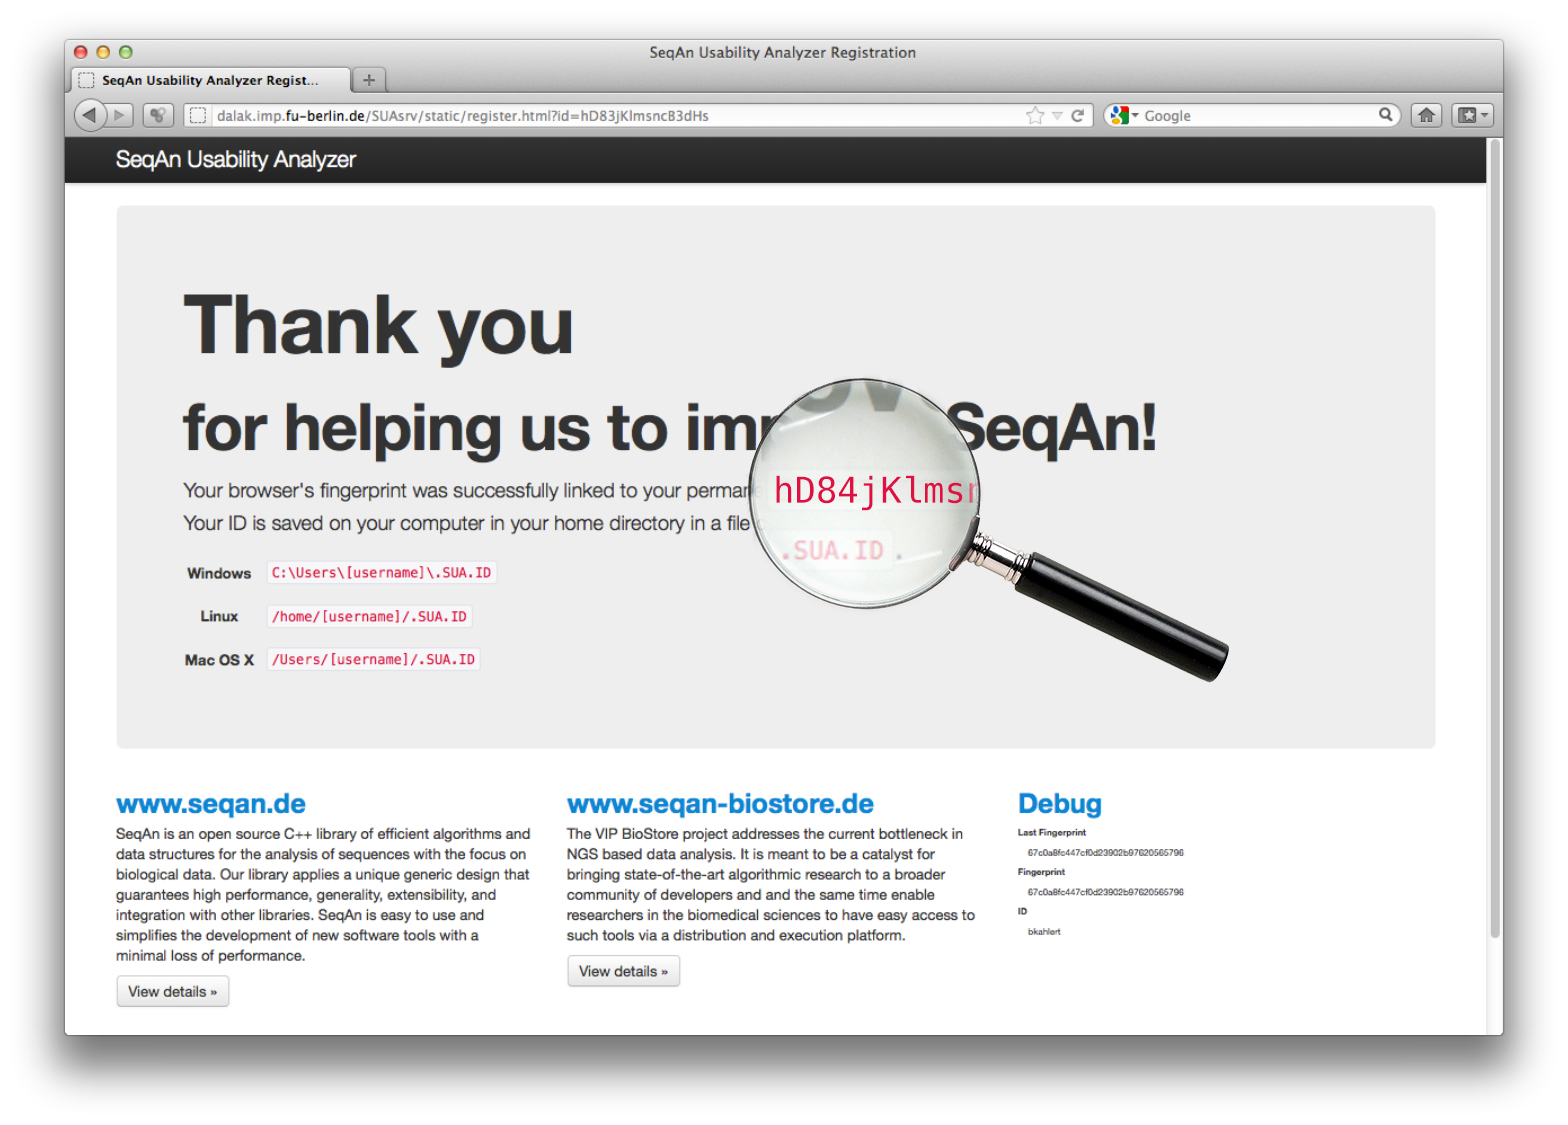
\includegraphics[width=0.75\linewidth]{Figures/apiua/activation.png}
  \caption{Bestätigung der Aktivierung der Datenerhebung}
  \label{fig:apiua-activation}
\end{figure}

Durch die ausschließliche Verwendung einer ID, setze ich das Prinzip der Pseudonymisierung um. Ein Rückschluss auf die Identität des Probanden ist so, stark erschwert. Ich hatte bei der Datenanalyse selbst mehrere Male das Bedürfnis, einen Probanden zu kontaktieren. Selbst mit dieser starken Motivation ist es mir nicht gelungen, die korrekte Person zu identifizieren.

Die Datenerhebung kann jederzeit vom Proband durch Löschen der Datei \texttt{.APIUA} eigenständig beendet werden.

\begin{furtherreading}[frametitle={Stabiles Browser-Fingerprinting}]
\label{subsec:browser-fingerprint}
Browser-Fingerprinting erfreut sich in der Online-Werbebranche großer Beliebtheit \citep{Bager:IDwRnNoQ} und verwendet diverse Merkmale, die der Browser (a) in seiner HTTP-Anfrage mitschickt oder (b) sich mit JavaScript auslesen lassen. Durch installierte Plugins, wie Flash oder Java, steigt der verwendbare Merkmalumfang weiter an. Ein Großteil, der weltweit eingesetzten Browser-Installationen, ist durch diese Merkmale eindeutig identifizierbar\footnote{\url{http://m.heise.de/newsticker/meldung/Fingerprinting-Viele-Browser-sind-ohne-Cookies-identifizierbar-1982976.html}\\\url{https://panopticlick.eff.org/browser-uniqueness.pdf}}.

Je mehr Merkmale für den Browser-Fingerprint verwendet werden, desto wahrscheinlicher ist eine eindeutige Erkennbarkeit. Allerdings steigt so auch die Wahrscheinlichkeit einer Veränderung des Browser-Fingerprints.

Um einen Browser dauerhaft zu identifizieren, benötigt man einen Mechanismus, der es einem erlaubt, den alten und den neuen Browser-Fingerprint in Erfahrung zu bringen.

Dazu muss zunächst der alte Browser-Fingerprint im Browser --- z.B. in Form eines Cookies --- gespeichert werden. Cookies (und alle anderen lokalen Speicherformen) setzen die Same-Origin-Policy um. Das heißt, dass ein, auf einer beliebigen  Seite \textit{example.com} eingefügtes Datenerhebungsscript von \textit{server.com}, nicht die Cookies der jeweils anderen Domain auslesen kann. Das Datenerhebungsscript arbeitet im Kontext von \textit{example.com}, muss aber Cookies im Kontext von \textit{server.com} ablegen, damit es Anwender, über mehrere Domains hinweg, verfolgen kann.

Um das zu erreichen, erzeugt mein Datenerhebungsscript im \textit{Document Object Model} von \textit{example.com} ein unsichtbares \textit{IFrame} und lädt darin eine speziell präparierte HTML-Seite von \textit{server.com}. Diese spezielle Seite verfügt selbst über ein JavaScript, das nun Cookies im Kontext von \textit{server.com} anlegen und so den alten Fingerprint im Browser speichern kann. Verändert sich nun der Browser-Fingerprint, kann \textit{server.com} den alten Fingerprint aus dem Cookie auslesen und die, unter dem alten Fingerprint gespeicherten Daten auf den neuen Fingerprint umschreiben.

Tatsächlich ist das Problem noch ein ganzes Stück komplexer. Für die Kommunikation zwischen der Seite und dem IFrame übergebe ich Daten über das \texttt{window.name}-Objekt\footnote{\url{https://bugzilla.mozilla.org/show_bug.cgi?id=444222}} und für die Datenablage verwende ich alle erdenklichen Speichermöglichkeiten (\textit{local storage}, \textit{flash cookies}, etc.), wie es das \textit{evercookie} \citep{Kamkar:FIOYXZjo} vormacht. Löscht der Anwender nicht sämtliche Speicherorte auf einmal, stellt \textit{evercookie} sicher, dass die gespeicherten Informationen wieder mit allen Speicherorten synchronisiert werden. Der Anwender kann die, in seinem Browser gespeicherten Informationen praktisch nicht löschen\footnote{\url{http://www.heise.de/newsticker/meldung/User-Tracking-Werbefirmen-setzen-bereits-haeufig-nicht-loeschbare-Cookie-Nachfolger-ein-2264381.html?wt_mc=rss.ho.beitrag.atom}}.
\end{furtherreading}

\begin{figure}
  \centering
    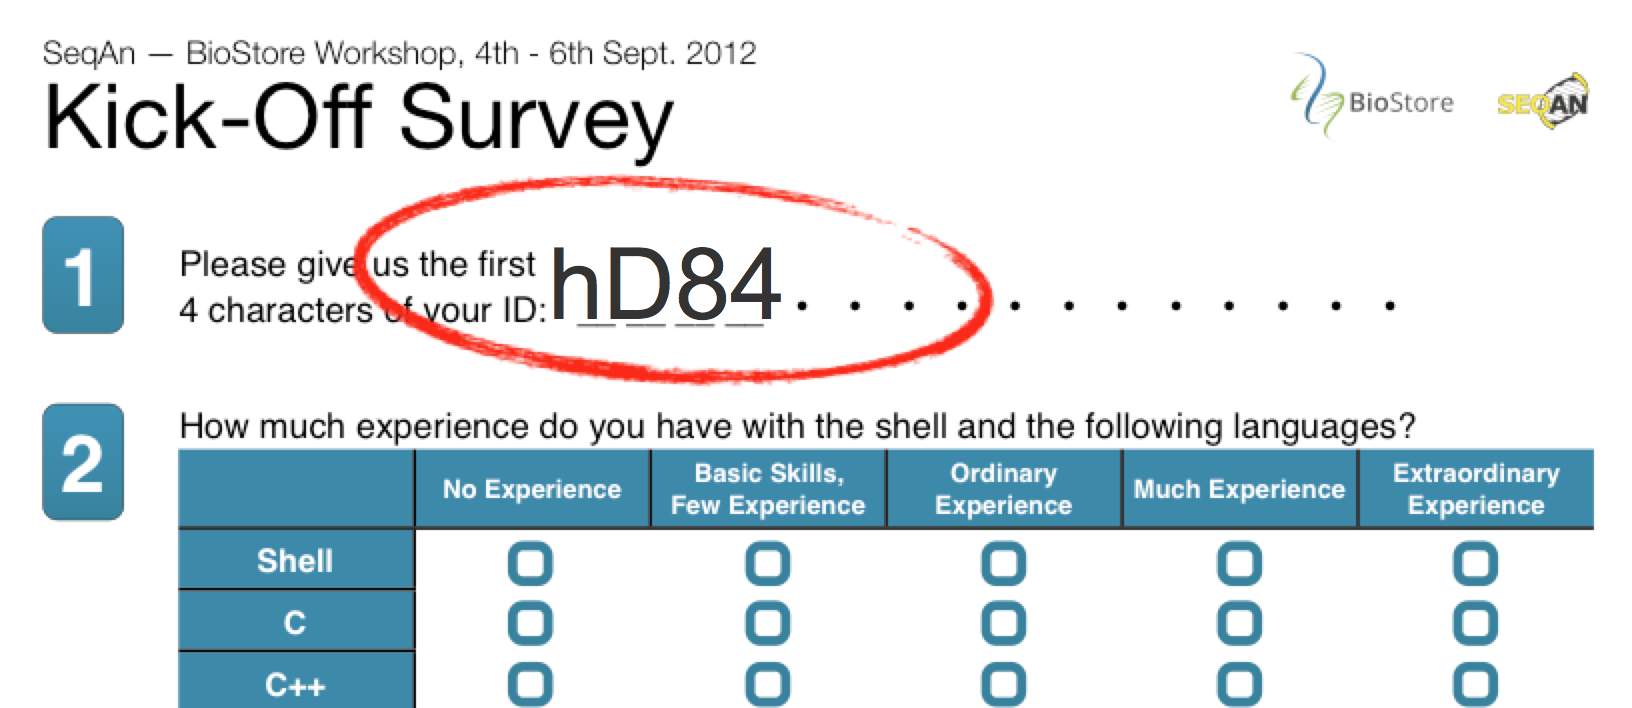
\includegraphics[width=0.75\linewidth]{Figures/survey-id.png}
  \caption{Eintragung der ID im Feedback-Zettel}
  \label{fig:survey-id}
\end{figure}
  
  
  
\subsubsection{Durchführung und Fazit}
\label{sec:phase2-programmierfortschritte-durchfuhrung}

Aktivitäten wurden auf den Webseiten für die Online-Dokumentation und für die Tutorials protokolliert.

Die Aufzeichnung der Programmierfortschritte fand bei allen Workshops ('11, '12 und '13), sowie bei zwei von drei PMSB-Praktika ('12, '13) statt. Des Weiteren konnte ich einen Langzeitprobanden gewinnen. Dieser Datensatz umfasst mehr als 1.200 Entwicklungsschritte. Insgesamt liegen Datensätze zu über 50 Probanden vor.

Zur Analyse der Datensätze kam die \gls{gtm} zum Einsatz. Wegen des hohen Aufwand zur Analyse dieser Daten, wurden nur wenige Datensätze betrachtet. Die Ergebnisse werden in den Abschnitten \ref{sec:phase4} und \ref{sec:Ergebnisse} vorgestellt.

Die hier präsentierte Datenerhebungsmethode unterscheidet sich von den, üblicherweise gebräuchlichen Videoaufzeichnungen \citep[vgl.][]{clarke:2006,LaToza:2007fj,Grill:2012jm,Piccioni:2013uq}. Es arbeitet Plattform- und Entwicklungsumgebung-übergreifend, erfordert keine Anpassungen am Arbeitsplatz der Probanden und eignet sich für Langzeitstudien, was die Beobachtung von Usability-Problemen erlaubt, die nicht in einem einzelnen Messpunkt zu finden sind oder erst nach einem längeren Gebrauch einer API auftreten. Technisch gesehen, könnte dieses Verfahren sogar vollkommen transparent, automatisiert und ohne jedes anwenderseitige Zutun eingesetzt werden.

Vergleichbare, manuell einzurichtende Datenerhebungen haben \cite{LaToza:2007fj,Layman:2008:MIU:1370114.1370133} implementiert. Dabei wurde jedoch \gls{eclipse} instrumentalisiert, was andere Entwicklungsumgebungen ausschließt. Der Vorteil besteht allerdings darin, dass mit einem \gls{eclipse}-Plugin auch feingranularere Ereignisse erfasst werden können. Browserzugriffe werden hingegen nicht von deren Datenerhebungen erfasst.

Die Datenerhebungsmethode wurde im Verlauf dieser Studie mehrfach verbessert. Während der ersten Datenerfassung wurden Schwächen deutlich, die beseitigt werden mussten. Diese Behebungen waren teilweise sehr aufwändig, da die bereits erhobenen Daten immer wieder auf aktualisierte Datenformate umgestellt werden mussten. Die folgende Auflistung nennt die wichtigsten Verbesserungen: \label{sec:datenerhebung-probleme}
\begin{itemize}
  \item Manche Anwender verwendeten mehrere SeqAn-Installationen oder mehrere Entwicklungsumgebungen. Die entsprechende Unterstützung musste implementiert werden, um unterschiedliche Programmentwicklungsverläufe unterscheiden zu können.
  \item Bei den ersten Datenerhebungen wurde die Zeitzone nicht mit erfasst. Dies führte bei einem Teilnehmer zu Problemen, da der Server eine andere Zeitzone verwendete und damit die verschiedenen Datenquellen zeitlich verschoben waren. Die Datenerhebung wurde um eine entsprechende Zeitzonen-Unterstützung ergänzt.
  \item Ursprünglich wurden nicht die geänderten Dateien, sondern nur das Dateien-Diff\footnote{\url{https://www.gnu.org/software/diffutils/}} übertragen. Bei fehlerhaften Datenerhebungen führte das dazu, dass die späteren Dateistände nur noch händisch oder gar nicht mehr rekonstruiert werden konnten.
  \item Fehler bei der Datenerhebung wurden nicht protokolliert. Eine entsprechende Protokollierung wurde implementiert. Auftretende Fehler werden nun an eine zuvor hinterlegte E-Mail-Adresse weitergeleitet.
  \item Die große Bandbreite an möglichen Konfigurationen auf Probandenseite, machte automatisierte Tests notwendig. Dieses Tests umfassen alle hier vorgestellten Datenquellen. Dabei kam das Code-Coverage-Tool \textit{EclEmma}\footnote{\url{http://www.eclemma.org}} zum Einsatz. Für das Testen der verschiedenen Browser verwendete ich \textit{Selenium}\footnote{\url{http://www.seleniumhq.org}}.
  \item Die Unterstützung von SSL-basierten Webseiten wurde implementiert, weil einige Webseiten sowohl über HTTP, als auch über HTTPS verfügbar sind.
  \item Die Datenerhebung wurde --- wo es möglich war --- parallelisiert und asynchron implementiert.
  \item Die Webseiten-Ereignisse \textit{FOCUS} und \textit{BLUR} wurden hinzugefügt, um besser nachvollziehen zu können, ob und welche Webseite bzw. Browser-Tab gerade gelesen wird.
\end{itemize}

Ein Problem konnte nicht gelöst werden: Der Erfolg oder Misserfolg von Kompilierversuchen konnte nicht protokolliert werden. Dies ist ohne größeren Aufwand nicht Plattform- und Entwicklungsumgebung-übergreifend möglich. Eine Option besteht darin, die verschiedenen Dateistände nachträglich zu kompilieren. Eine zuverlässige Rekonstruktion würde jedoch die Bereitstellung der entsprechenden Arbeitsumgebungskonfigurationen erfordern, was seine eigenen Probleme mit sich bringt.



\subsection{Zusammenfassung}
\label{sec:phase2-fazit}

In diesem Abschnitt habe ich ein umfassendes Datenerhebungsverfahren vorgestellt.

Durch die Erfassung von Programmierfortschritten erlaubt dieses Datenerhebungsverfahren, im Gegensatz zu fast allen mir bekannten Arbeiten, Langzeitstudien durchzuführen. Die erhobenen Daten werden nicht durch die Erzwingung der Arbeit an einem, für eine Datenerhebung vorbereiteten Arbeitsplatz verfälscht. Darüber hinaus wird die Datenerhebung durch das einfache Anlegen bzw. Löschen einer Datei aktiviert bzw. deaktiviert und der Anwender nicht abgelenkt.

Die objektiven Daten werden durch subjektive Daten ideal ergänzt, da sie teilweise verschiedenartige Usability-Probleme beherbergen. Subjektive Daten können außerdem Orientierung für die Analyse der objektiven Daten geben. Sie werden mit Hilfe einer Gruppendiskussion und dem hier vorgestellten Cognitive-Dimensions-Fragebogen erhoben.

Das Datenerhebungsverfahren wird meinen speziellen Anforderungen gerecht. Durch die nicht beeinflussbaren Datenerhebungsmöglichkeiten, war eine besonders hohe Reichhaltigkeit vonnöten, denn weitere Datenerhebungen im Sinne des \textit{theoretischen Samplings} waren nicht ohne weiteres möglich. Dieser Ansatz ist tolerabel, denn einerseits umfassen die Daten bereits verschiedene Datenquellen, was dem Triangulierungsgütekriterium entgegenkommt und andererseits erlaubt die Reichhaltigkeit der Daten weitere Analysen unter einem anderen Betrachtungswinkel. 

Die Teilnehmer der Workshops und PMSB-Praktika repräsentieren hinreichend die SeqAn-Anwendergruppe.

Die verschiedenen Datenerhebungen wurden bei den folgenden Veranstaltungen wie folgt durchgeführt:
\begin{description}
  \item[Workshops] \hfill
  \begin{description}
    \item[Workshop'11] \textit{13.-15.09.2011}
    \begin{description}
%      \item[Fragebögen] von xx Teilnehmer
      \item[Programmierfortschritte] von 13 Teilnehmern
    \end{description}
    
    \item[Workshop'12] \textit{04.-06.09.2012}
    \begin{description}
%      \item[Interviews] mit keinem der Teilnehmer, da es wegen der hohen Veranstaltungsdichte keinen Raum dazu gab
      \item[Gruppendiskussion] von rund 20 Teilnehmern
      \item[Programmierfortschritte] von 14 Teilnehmern
    \end{description}
     
    \item[Workshop'13] \textit{17.-19.09.2013}
    \begin{description}
      \item[Cognitive-Dimensions-Fragebogen] von 10 Teilnehmer
      \item[Programmierfortschritte] von 16 Teilnehmern
    \end{description}
  \end{description}
  
  \item[PMSB] \hfill
    \begin{description}
    \item[PMSB'12] \textit{05.2012}
    \begin{description}
%      \item[Interviews] mit 4 Teilnehmer
      \item[Programmierfortschritte] von 6 Teilnehmern
    \end{description}
    
    \item[PMSB'13] \textit{04.2013}
    \begin{description}
      \item[Fragebögen] von xx Teilnehmer
      \item[Programmierfortschritte] von 10 Teilnehmern
    \end{description}
    
    \item[PMSB'14] \textit{04.2014}
    \begin{description}
      \item[Programmierfortschritte] nicht erhoben
    \end{description}
  \end{description}
  
  \item[Langzeitprobanden] \hfill
  \begin{description}
    \item[Programmierfortschritte] von einem Teilnehmer %Langzeitproband David Meyer gewonnen (03.07.2012, brbym28nz827lxic) über 1200 Revisionen
  \end{description}
\end{description}

\bigskip

Da nun die Daten erhoben werden konnten, dürfte der Analyse Selbiger mit Hilfe der \gls{gtm} nichts im Weg stehen. Allerdings unterstützte kein gängiges Datenanalysewerkzeug die qualitative Analyse dieser hoch-strukturierten Daten. Aus diesem Grund musste ich selbst ein Werkzeug entwickeln, das ich im folgenden Abschnitt vorstelle.

In Phase 4 (\sref{sec:phase4}) werde ich schließlich die eigentliche Forschung mit Hilfe der \gls{gtm} und meinem Datenanalysewerkzeug besprechen.
\section{Phase 3: Entwicklung des API Usability Analyzers}
\label{sec:apiua}

Der \textit{\acrfull{apiua}} (siehe Abbildungen \ref{fig:apiua-splash} und \ref{fig:apiua-opencoding-devel}) ist das Werkzeug, mit dessen Hilfe ich die von mir erhobenen und im vorangegangenen Abschnitt beschriebenen Daten analysiert und die im nächsten Kapitel vorgestellten Forschungsergebnisse erarbeitet habe.

Dabei war das Werkzeug zunächst als reine Visualisierungslösung für die spezielle Form der \textit{Programmierfortschritte}-Datenquelle gedacht. Erst durch die Notwendigkeit, die \gls{gtm} direkt dieser Software anwenden zu können, kam sukzessive die Unterstützung der verschiedenen Aktivitäten dieser Forschungsmethode, wie die verschiedenen Kodierungsarten, hinzu. Eine Einführung in die \gls{gtm} findet sich im \sref{sec:gtm}. Die Entwicklung von \gls{apiua} im zeitlichen Verlauf ist im \sref{sec:verlauf} dargestellt.

Der \acrlong{apiua} besteht aus den folgenden drei Komponenten:
\begin{description}
  \item[API Usability Analyzer] wird vom Forscher für die eigentliche Forschungsarbeit verwendet.\footnote{\url{https://github.com/bkahlert/api-usability-analyzer}}
  \item[API Usability Analyzer Client] läuft auf den Arbeitsplätzen der Probanden und ist für die klientseitige Datenerhebung zuständig. Diese Komponente wird genauer online\footnote{\url{https://github.com/bkahlert/api-usability-analyzer-client-python}} und im \sref{sec:apiua-client} beschrieben.
  \item[API Usability Analyzer Server] sammelt die durch Clients erhobenen objektiven Rohdaten, die dann, mit Hilfe des Datenanalysewerkzeugs, verarbeitet werden können. Diese Komponente wird genauer online\footnote{\url{https://github.com/bkahlert/api-usability-analyzer-server-java-ee}} und im \sref{sec:apiua-server} beschrieben.
\end{description}

Dieser Abschnitt beschränkt sich auf das von mir entwickelte Datenanalysewerkzeug selbst. \aref{app:apiua} ergänzt diese Beschreibung, durch eine nähere Erläuterung einzelner Komponenten.

\begin{figure}[ht!]
  \centering
    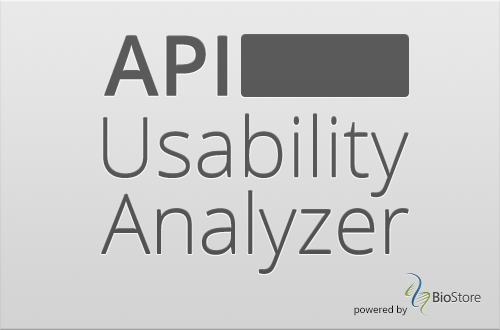
\includegraphics[width=0.4\linewidth]{Figures/apiua/splash.png}
  \caption[APIUA: Startbildschirm]{Der Startbildschirm von \gls{apiua}}
  \label{fig:apiua-splash}
\end{figure}

\newgeometry{inner=2cm,outer=1.5cm,top=1.5cm,bottom=1.5cm}
\thispagestyle{empty}
\begin{landscape}
\begin{figure}
  \centering
    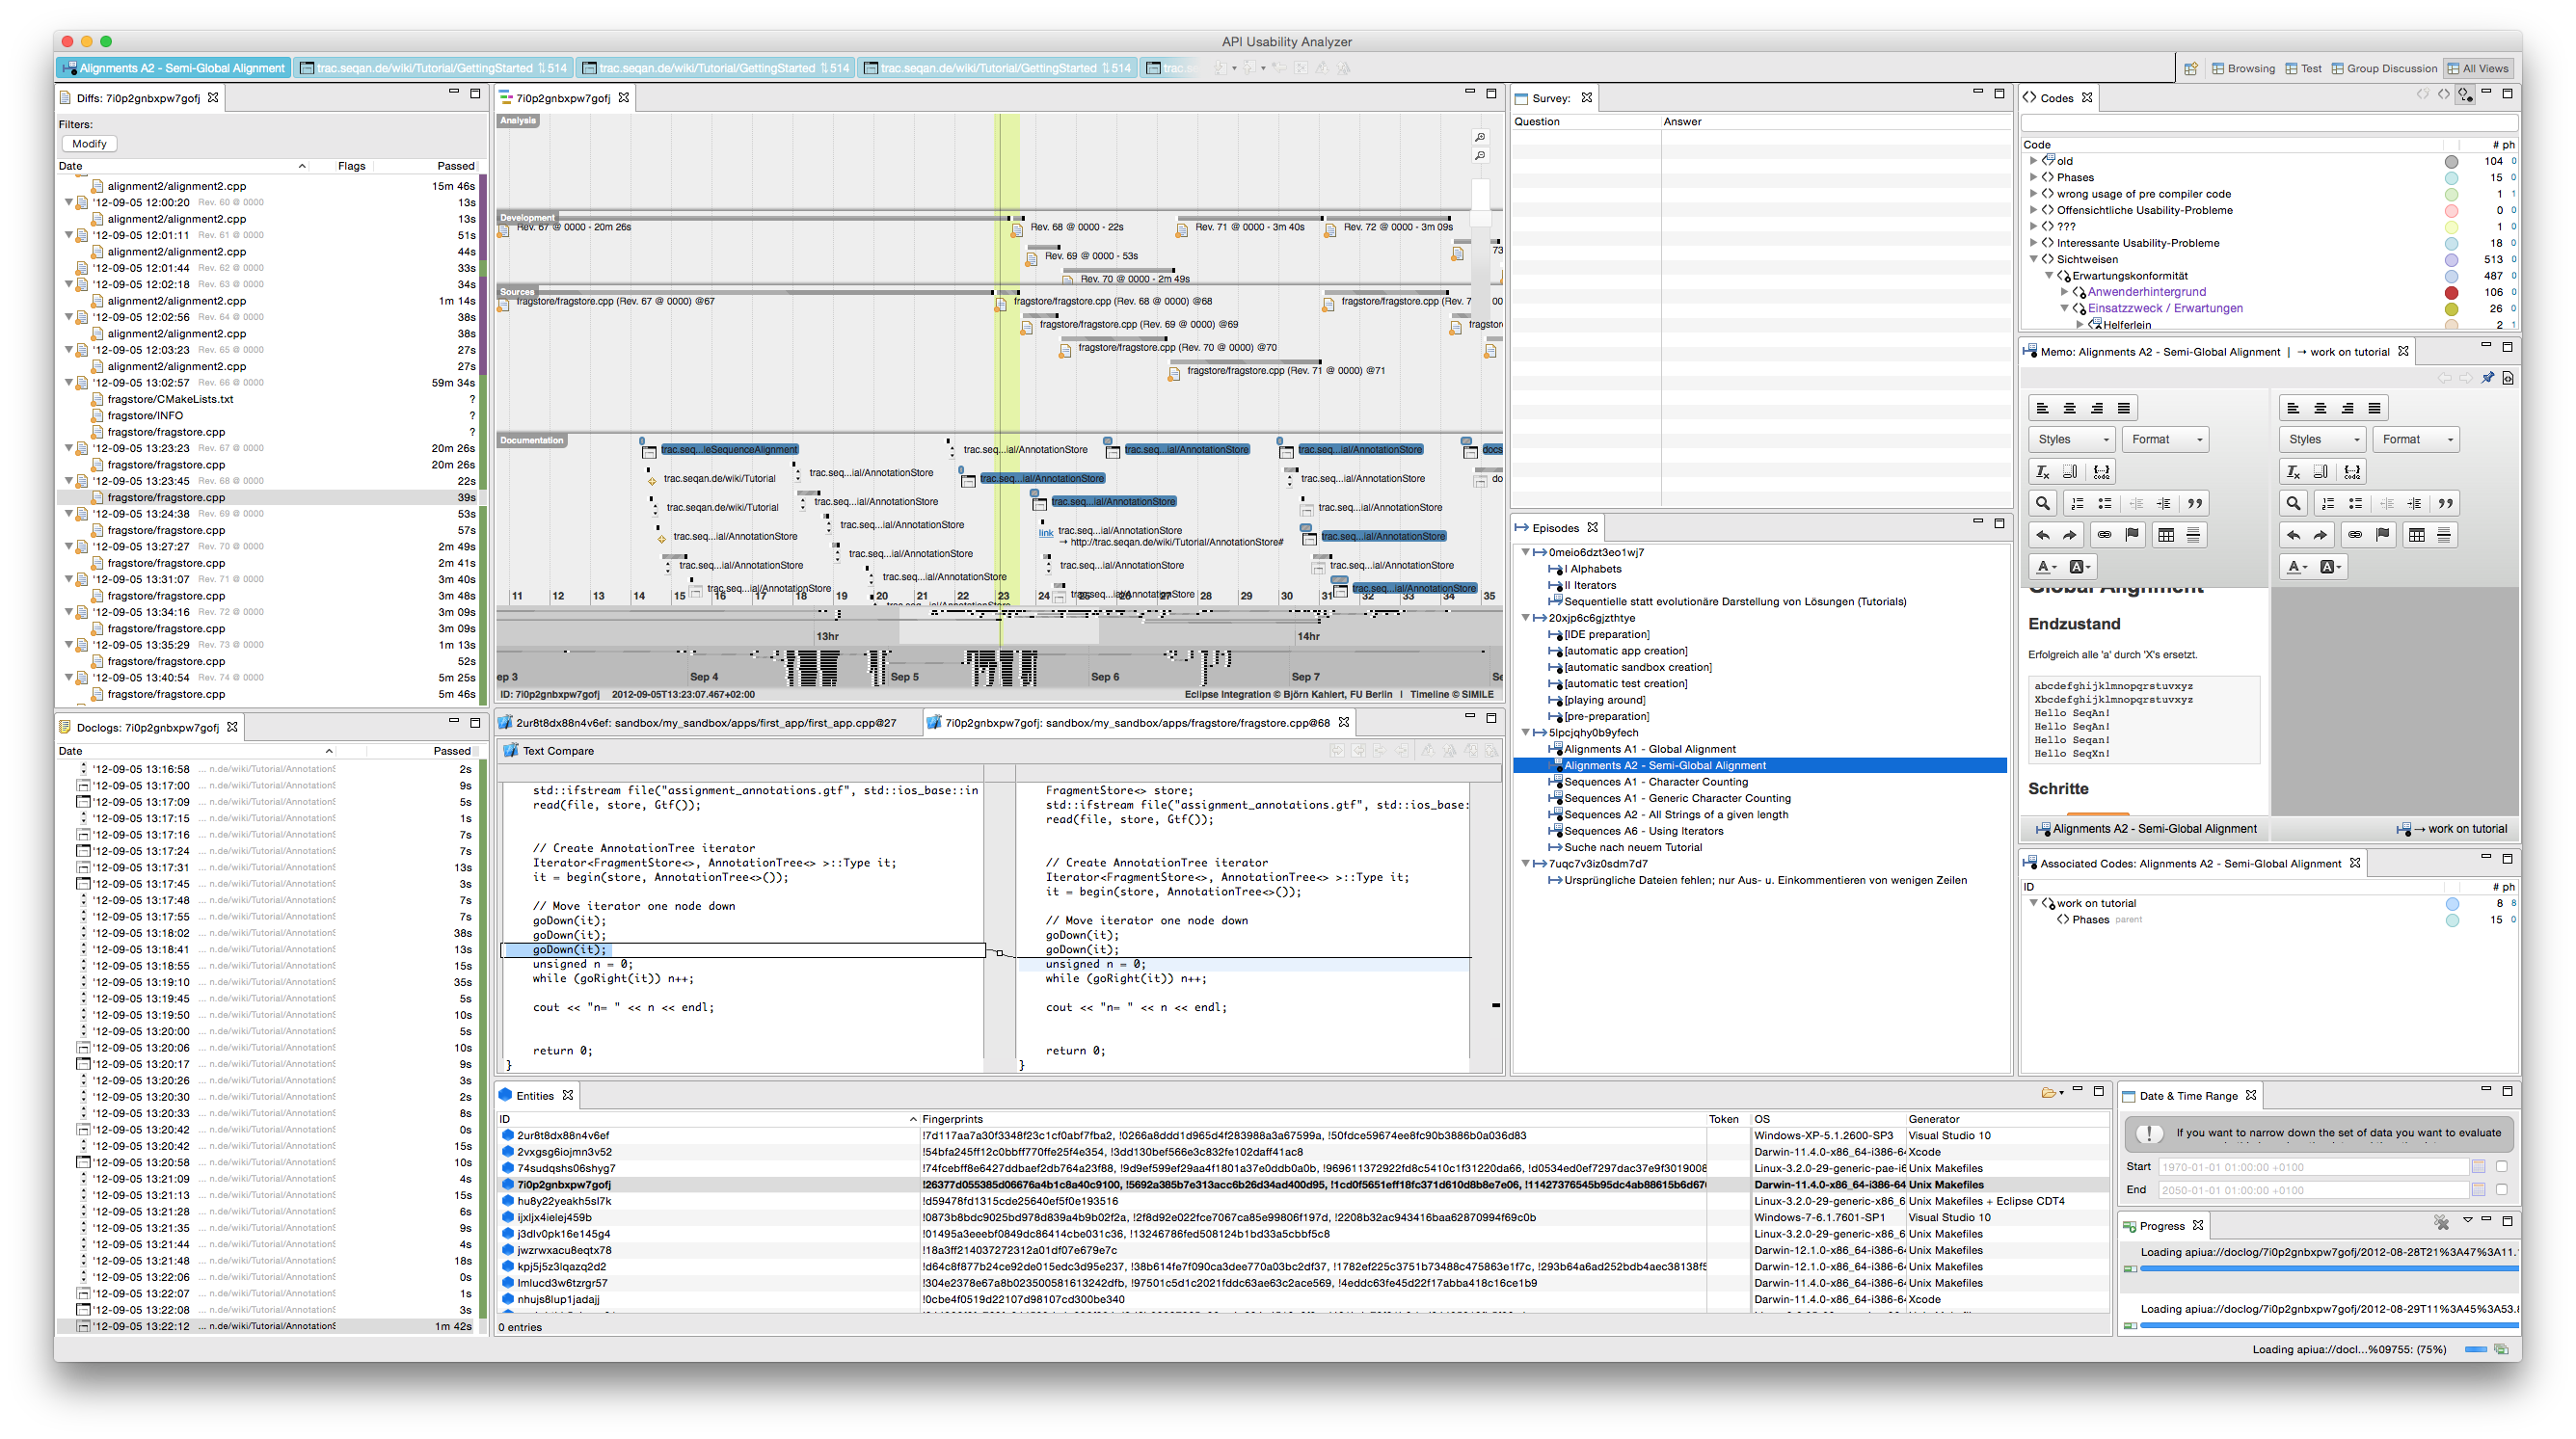
\includegraphics[width=1.0\linewidth]{Figures/apiua/opencoding-devel.png}
  \caption[APIUA: Offenes Kodieren]{Dieser Screenshot von \gls{apiua} zeigt eine typische Sitzung mit Fokus auf offenes Kodieren. In diesem Fall werden Programmierfortschritte des Probanden mit der ID \texttt{7i0p2gnbxpw7gofj} analysiert.}
  \label{fig:apiua-opencoding-devel}
\end{figure}
\end{landscape}
\restoregeometry






\subsection{Motivation}

Je umfassender ein zu analysierendes Datenmaterial ist, desto mehr zwängt sich ein computergestütztes Verfahren auf. Auf dem Markt gibt es verschiedene Anwendungen, die sich grundsätzlich für die Verwendung der \gls{gtm} eignen. Zu den führenden \textit{CAQDAS}\footnote{Computer-unterstützte qualitative Datenanalysesoftware\\(\textit{\textbf{c}omputer \textbf{a}ssisted/\textbf{a}ided \textbf{q}ualitative \textbf{d}ata \textbf{a}nalysis \textbf{s}oftware})}-Vertretern gehören \textit{MAXQDA}\footnote{\url{http://www.MAXQDA.de}} und \textit{ATLAS.ti}\footnote{\url{http://atlasti.com/de/}} \citep{ann2007using}. Beide Programme dienen dem Zweck der qualitativen Datenanalyse und eignen sich für die \gls{gtm} \citep{Wolf:2014vv,Dresing:2006te,ann2007using}.

Bedauerlicherweise haben alle großen CAQDAS-Vertreter nicht zu vernachlässigende Schwächen in Bezug auf ihren Einsatz als \gls{gtm}-Software \citep{ann2007using}. Axiales Kodieren wird von \textit{MAXQDA} überhaupt nicht \citep{Wolf:2014vv} und von anderen Werkzeugen nur im Umfang einer Zeichenfläche unterstützt \citep{ann2007using}. Im letzteren Fall verlieren, auf eine Zeichenfläche positionierte Kodes sogar die Information, woher sie kommen und werden --- im Falle von Kode-Änderungen --- nicht mehr aktualisiert . Einzig \textit{ATLAS.ti} speichert die Referenz auf eine verwendete Relation in ihrem Netzwerk-Editor \citep{ann2007using}. Bezüglich \textit{ATLAS.ti} schildern meine Arbeitsgruppenkollegen \cite{Schenk:3LdEjzOu} und \cite{Zieris:yCXyxVc9} die folgenden Probleme bei ihrer Forschungsarbeit:

\begin{description}
  \item[Funktionale Probleme] \hfill
  \begin{itemize}
    \item Offenes Kodieren wird erschwert, weil Kodes nur sehr eingeschränkt\footnote{Mit Hilfe von Superkodes, Familien und Superfamilien gibt es eine Möglichkeit der Gruppierung \citep{MuhlmeyerMentzel:2011vs}, die aber von den beiden Kollegen wegen ihrer schwierigen Handhabung gemieden wird. Beispielsweise können Familien nicht während der axialen Kodierung verwendet werden.} gruppiert und gar nicht sortiert werden können. Zudem sind Referenzen innerhalb von Memos nicht möglich. Im Zusammenhang mit den unten genannten Defekten resümiert \cite{Zieris:yCXyxVc9}, dass es ``kein[en] Überblick beim Open Coding'' gibt. Weiterhin fehlt die Möglichkeit, zwei Akteure separat zu kodieren, was den Kodierprozess bei der Analyse von Paarprogrammierungssitzungen verkompliziert. Anfang und Ende einer Quotation können nicht verändert werden.
    \item Axiales Kodieren ist nur eingeschränkt möglich, da es für jeden Kode maximal eine \glslink{ac}{axiale Kodierung} bzw. ein \glslink{acm}{axiales Kodiermodell} geben darf. Eine Übersicht über alle existierenden \glslink{ac}{axialen Kodierungen} und \glslink{acm}{axialen Kodiermodellen} gibt es nicht. Die Bedienung des Editors selbst gestaltet sich schwierig. So ist es nicht möglich, als Pfeilverbindungen dargestellte Relationen auszublenden oder auf eine andere Weise in ihrer Gestalt zu verändern. Die beiden Befragten nutzen aus diesen Gründen die entsprechende Funktionalität von \textit{ATLAS.ti} nicht bzw. nur in seltenen Fällen und weichen auf andere Programme aus (\textit{OmniGraffle}\footnote{\url{https://www.omnigroup.com/omnigraffle}} bzw. \textit{Microsoft Visio}\footnote{\url{http://products.office.com/de-de/visio}}). In \textit{ATLAS.ti} gibt es die Möglichkeit Kodes zu verankern. Diese Möglichkeit besteht aber nicht für Relationen zwischen Kodes.
  \end{itemize}
  
  \item[Bedienschwierigkeiten] \hfill
  \begin{itemize}
    \item Es ist schwer, den Fokus auf das gerade betrachtete Datum zu behalten, denn verschiedene Operationen führen dazu, dass sich unbeabsichtigte Änderungen der Ansicht ergeben. Dazu gehört beispielsweise das bloße Klicken auf eine Quotation, das die Zeitleiste springen lässt.
    \item Die Arbeit ist schwerfällig, weil viele Ansichten exklusiv sind und der Wechsel zwischen ihnen ``zeitraubend'' ist. Dies behindert insbesondere das \textit{ständige Vergleichen}. Beispiel: Entweder kodiert man sein Videomaterial oder man interessiert sich für die Eigenschaften eines Codes. Die dazu jeweils notwendigen Ansichten können nicht parallel geöffnet sein.
    \item Die Suchfunktion wird nur eingeschränkt wegen ihrer komplizierten Syntax genutzt.
    \item Der Zustand der Arbeitsumgebung wird nicht vollständig gespeichert. Nach einem Neustart der Anwendung muss --- bevor die Arbeit fortgesetzt werden kann --- der alte Zustand wiederhergestellt werden.  
  \end{itemize}
  
  \item[Defekte / Sonstiges] \hfill
  \begin{itemize}
  	\item Die Identifikatoren von Kodes werden von \textit{ATLAS.ti} wiederverwendet. Wird ein Kode gelöscht und ein neuer Kode erzeugt, kann es passieren, dass der neue Kode den Identifikator des alten Kodes erhält. Verweise auf den alten Kode zeigen dann fälschlicherweise auf den neuen Kode. 
    \item Existieren auf einem Abschnitt auf der Zeitliste zu viele Quotations, werden diese nicht mehr vollständig sichtbar aufgezählt sondern abgeschnitten.
%    \item Die Zeitpunkte, an denen die Analysedaten gesichert werden, sind unbestimmt.
%    \item Gleiche Aktionen werden an verschiedenen Stellen des Programm mit unterschiedlichen Ikonen symbolisiert. Beispiel: Die Speichern-Operation wird einmal als Diskette und einmal als Häkchen dargestellt.
  \end{itemize}
\end{description}

Die Verwendung eines der existierenden Produkte empfiehlt sich auch aus einem weiteren wichtigen Grund nicht: Die im Rahmen dieser Arbeit erhobenen Daten sind hochstrukturiert. Ihr Informationsgehalt ist für einen Menschen nur schwer zu erfassen. Warum das so ist, sollen die beiden folgenden Beispiele veranschaulichen.



\subsection{Beispiel: Diff-Dateien}

Eine Diff-Datei beschreibt sämtliche vom Probanden gemachten Dateiänderungen zwischen zwei Kompilierversuchen innerhalb des SeqAn-Verzeichnisses.\\
Oder einfacher ausgedrückt: Wenn ein Proband in der Datei \texttt{first\_app.cpp} eine Zeile Code hinzufügt und anschließend in seiner Entwicklungsumgebung die Anwendung ausführen will, wird die folgende Datei aufgezeichnet:

\begin{center}
%\inputminted[firstline=3, lastline=6]{diff}{/Users/bkahlert/promotion/workshop12/workshop2012-data-20120906/diff/2ur8t8dx88n4v6ef/2ur8t8dx88n4v6ef_r00000007_2012-09-04T13-33-07+0200.diff}
\begin{minted}[linenos, firstnumber=1]{diff}
diff -u -r -N -x '*.o' -x Thumbs.db -x .DS_Store -x CMakeCache.txt -x misc/seqan_instrumentation/userdata/id.txt -x C:/Software/SeqAn/seqan/misc/seqan_instrumentation/userdata/id.txt -x misc/seqan_instrumentation/userdata/2ur8t8dx88n4v6ef_stats.txt -x C:/Software/SeqAn/seqan/misc/seqan_instrumentation/userdata/ 2ur8t8dx88n4v6ef_stats.txt -x .svn -x bin -x build -x util -x misc -x docs -x docs2 -x extras -x core -x misc/seqan_instrumentation/bin -x C:/Software/SeqAn/seqan/misc/seqan_instrumentation/bin -x misc/seqan_instrumentation/last_revision_copy -x C:/Software/SeqAn/seqan/misc/seqan_instrumentation/last_revision_copy -x misc/seqan_instrumentation/last_revision_copy -x C:/Software/SeqAn/seqan/misc/seqan_instrumentation/last_revision_copy -x misc/seqan_instrumentation/userdata -x C:/Software/SeqAn/seqan/misc/seqan_instrumentation/userdata -x misc/seqan_instrumentation/userdata -x C:/Software/SeqAn/seqan/misc/seqan_instrumentation/userdata ./misc/seqan_instrumentation/last_revision_copy/sandbox/my_sandbox/ apps/first_app/first_app.cpp ./sandbox/my_sandbox/apps/first_app/first_app.cpp
--- ./misc/seqan_instrumentation/last_revision_copy/sandbox/my_sandbox/ apps/first_app/first_app.cpp	2012-09-04 13:32:34.281250000 +0200
+++ ./sandbox/my_sandbox/apps/first_app/first_app.cpp	2012-09-04 13:33:05.968750000 +0200
@@ -13,6 +13,8 @@
 	
 	readRecord(id, seq, seqStream);
 
+	std::cout << id << '\t' << seq << '\n';
+
 	seqan::CharString mySeqanString = "Done.";
     std::cout << mySeqanString << std::endl;
 	return 1;
\end{minted}
\captionof{listing}[Beispiel: Einfache Diff-Datei]{Einfache Diff-Datei, die zwei hinzugefügte Code-Zeilen dokumentiert}
\label{lst:diff-file}
\end{center}
  
Welche Informationen können wir der Diff-Datei \texttt{2ur8t8dx88n4v6ef\_2b2f\_\allowbreak 2012-09-04T\allowbreak 13-33-07+0200.diff} entnehmen?
  
\begin{center}
  \begin{tabularx}{\linewidth}{X X X}
  \textbf{Information} & \textbf{Fundort} & \textbf{Wert} \\
  \midrule
  ID des Probanden & Diff-Dateiname & \texttt{2ur8t8dx88n4v6ef} \\
  Hash der Entwicklungsumgebung & Diff-Dateiname & \texttt{2b2f} \\
  Zeitpunkt des Kompilierversuchs & Diff-Dateiname & 04.09.2012, 13:33:07 \\
  Zeitpunkt der letzten Änderung an \texttt{first\_app.cpp} & Zeile 3 & 04.09.2012, 13:33:06 \\
  Für die Änderung beanspruchte Zeit & Differenz Zeilen 2 \& 3 & rund 32s \\
  Code-Änderungen & Zeilen 8-9 & Ausgabe und Leerzeile \\
  Kompiliererfolg & Infrastruktur nachstellen und selbst kompilieren & Die Datei kompiliert erfolgreich. \\
  \end{tabularx}
  \captionof{table}{In einer Diff-Datei enthaltene Informationen}
  \label{tab:DiffData}
\end{center}
  
\autoref{tab:DiffData} beschreibt, welcher Informationsgehalt in einer Diff-Datei steckt. Die Tabelle und die Diff-Datei veranschaulichen aber auch, wie schwer diese Informationen, bereits bei einem kleinen Beispiel, fehlerfrei zu extrahieren sind.
  
Damit nicht genug: Die Information \textit{für die Änderung beanspruchte Zeit} ist falsch berechnet. Richtig wäre es, anstelle der vorletzten Bearbeitung von \texttt{first\_app.cpp} den vorangegangen Kompilierversuch zu verwenden. Es soll  nicht erfasst werden, wie viel Zeit die letzte Bearbeitung einer Datei zurücklag, sondern wie viel Zeit der Anwender (vermutlich) innerhalb einer Iteration auf eine Datei verwendete. Diese Zeitspanne ist also maximal so lang, wie die Iteration selbst. Nie länger.
  
Für die korrekte Berechnung dieses Maßes wird also neben der betrachteten Diff-Datei auch ihr Vorgänger benötigt. Ähnlich verhält es sich mit dem Umstand, dass eine Diff-Datei nur die geänderten und deren Nachbarzeilen enthält. Möchte man den gesamten Inhalt zum Zeitpunkt des Kompilierversuchs wissen, muss man die lückenlose Historie aller Änderungen betrachten. Auch dann ist noch nichts darüber gesagt, ob die Datei tatsächlich kompiliert und wenn nicht, welcher Grund dafür verantwortlich ist.\footnote{Inzwischen werden zur Datenerhebung die vollständigen, geänderten Dateien und nicht mehr deren Diffs übertragen. Dennoch veranschaulicht dieses Beispiel, wie komplex das Lesen von Rohdaten ohne Werkzeugunterstützung sein kann.}

Noch unerwähnt blieben Konstellationen, die potentiell selten auftreten, dann aber besonders relevant sind, leicht übersehen werden und zu Fehlinterpretationen führen können. In einem Fall hatte eine vom Probanden veränderte Datei ein Modifikationsdatum, das weit zurücklag --- weiter als das zuvor dokumentierte Datum. Ein Vergleich aller vorangegangenen Dateiänderungen zeigte, dass der Proband eine alte Version der Datei wiederhergestellt hatte. Eine Operation, die man durch das bloße Betrachten des Dateiinhalts wahrscheinlich nicht erkannt hätte. 

Zu den allgemein anerkannten Grundprinzipien / Praktiken der \gls{gtm} gehört das \textit{ständige Vergleichen} \citep{strauss1990basics,corbin2014basics,Salinger:2013vd,Glaser:1967ts}\footnote{Der Vollständigkeit halber sei erwähnt, dass \cite{Mey2007} eine ``Akzentverlagerung'' von der ``constant comparison method'' hin zur ``Dimensionalisierung'' bei Strauss (und Corbin) beobachten.}. Es ist zu befürchten, dass die \gls{gtm}-Praktiken --- durch eine aufwändige, händische und damit fehlerträchtige Datenaufbereitung --- weniger sorgfältig angewendet werden und so die Qualität der \gls{gt} sinkt.
  
Durch technische Unterstützung können alle genannten Informationen automatisch aus einem Datum extrahiert und so aufbereitet werden, dass sie durch den Forscher einfacher verarbeitet werden können. \autoref{fig:AnalysisDiff} zeigt, wie alle, in \autoref{tab:DiffData} aufgelisteten Informationen visuell in \gls{apiua} dargestellt werden.
  
\begin{figure}
  \centering
    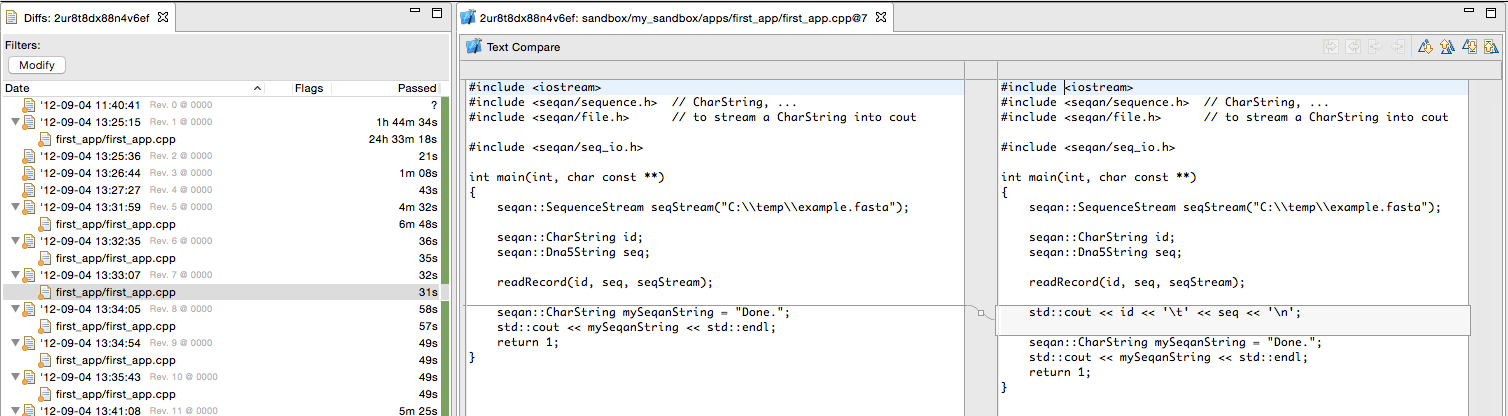
\includegraphics[width=1.0\linewidth]{Figures/AnalysisDiff.png}
  \caption[Beispielhafte Diff-Datei]{Dieser \gls{apiua}-Bildschirmausschnitt zeigt den Probanden \texttt{2ur8t8dx88n4v6ef}. Zu sehen sind im linken Drittel die ID des Probanden (im Tab), seine Kompilierversuche (Knoten erster Ordnung), alle bearbeiteten Dateien (Kindknoten), deren Kompiliererfolg (grüne, gelbe oder rote Icon-Annotation) und die auf sie verwendete Zeit. \\Im rechten Teil des Ausschnitts kann man die aktuell betrachtete Datei vollständig in ihrem vorangegangenen und aktuellen Zustand sehen. Die Codeänderungen sind grafisch hervorgehoben.}
  \label{fig:AnalysisDiff}
\end{figure}



\subsection{Beispiel: Doclog-Datei}
\label{sec:doclog}

Eine Doclog\footnote{\textbf{doc}umentation \textbf{log}}-Datei dokumentiert alle Zugriffe/Ereignisse auf die, im Internet bereitgestellte SeqAn-Dokumentation. Diese Dokumentation besteht hauptsächlich aus der Dokumentation selbst und den Tutorials.

Die Erfassung der Dokumentationszugriffe soll schwer nachvollziehbare Entwicklungsschritte zwischen zwei Kompilierversuchen vereinfachen. So können größere Code-Einfügungen bedeuten, dass dem Probanden ein Licht aufgegangen ist. Sie können aber auch bedeuten, dass der eingefügte Code schlicht von der Online-Dokumentation kopiert wurde. Letztere Interpretation kann aber nur zuverlässig vollzogen werden, wenn man dafür triftige Indizien hat. 

\begin{center}
\usemintedstyle{bw}
\begin{minted}[linenos=true,firstnumber=481]{sh}
2012-09-04T14:14:23.729+02:00 READY http://trac.seqan.de/wiki/Tutorial/ GettingStarted 160.45.233.238 - 0 0 1350 612
2012-09-04T14:14:26.774+02:00 SCROLL http://trac.seqan.de/wiki/Tutorial/ GettingStarted 160.45.233.238 - 0 228 1350 612
2012-09-04T14:14:27.463+02:00 LINK-http://trac.seqan.de/wiki/Tutorial/ GettingStarted/WindowsVisualStudio http://trac.seqan.de/wiki/Tutorial/ GettingStarted 160.45.233.238 - 0 228 1350 612
2012-09-04T14:14:27.784+02:00 UNLOAD http://trac.seqan.de/wiki/Tutorial/ GettingStarted 160.45.233.238 - 0 228 1350 612
2012-09-04T14:14:28.804+02:00 READY http://trac.seqan.de/wiki/Tutorial/ GettingStarted/WindowsVisualStudio 160.45.233.238 - 0 147 1350 612
2012-09-04T14:14:35.196+02:00 SCROLL http://trac.seqan.de/wiki/Tutorial/ GettingStarted/WindowsVisualStudio 160.45.233.238 - 0 3420 1350 612
2012-09-04T14:14:49.711+02:00 SCROLL http://trac.seqan.de/wiki/Tutorial/ GettingStarted/WindowsVisualStudio 160.45.233.238 - 0 4104 1350 612
2012-09-04T14:14:53.414+02:00 SCROLL http://trac.seqan.de/wiki/Tutorial/ GettingStarted/WindowsVisualStudio 160.45.233.238 - 0 3876 1350 612
2012-09-04T14:15:00.302+02:00 SCROLL http://trac.seqan.de/wiki/Tutorial/ GettingStarted/WindowsVisualStudio 160.45.233.238 - 0 3648 1350 612
2012-09-04T14:15:06.149+02:00 BLUR http://trac.seqan.de/wiki/Tutorial/ GettingStarted/WindowsVisualStudio 160.45.233.238 - 0 3648 1350 612
2012-09-04T14:15:21.071+02:00 FOCUS http://trac.seqan.de/wiki/Tutorial/ GettingStarted/WindowsVisualStudio 160.45.233.238 - 0 3648 1350 612
\end{minted}
\captionof{listing}[Beispiel: Auszug aus einer Doclog-Datei]{Auszug aus einer Doclog-Datei}
\label{lst:doclog-file}
\end{center}

Die Doclog-Datei ist eine Tabulator-separierte Liste. Ihre Spalten sind:

\begin{description}
	\item[DateTime] Zeitstempel in ISO8601
	\item[Action] Ereignis (READY, UNLOAD, FOCUS, LINK, SCROLL, etc.)
	\item[URI] Adresse der geöffneten Seite
	\item[IP] IP des Anwenders
	\item[ProxyIP] Proxy-IP des vom Anwender verwendeten HTTP-Proxies
	\item[ScrollX] Scrollposition X-Achse in Pixeln (px) vom oberen Rand des Dokuments
	\item[ScrollY] Scrollposition Y-Achse in Pixeln (px) vom linken Rand des Dokuments
	\item[Width] Breite des Browser-Ansichtsbereichs (Viewport) in Pixeln (px)
	\item[Height] Höhe des Browser-Ansichtsbereichs (Viewport) in Pixeln (px)
\end{description}

Die in der Doclog-Datei dokumentierte Nutzung der Online-Dokumentation durch den Probanden zeigt also, dass er das Tutorial \textit{Getting Started} um 14:14 Uhr öffnete (Zeile 1) und anschließend vertikal um 228px nach unten scrollte (Zeile 2). Zeile 3 zeigt, dass er den Link auf die SeqAn-Installationsanleitung für Visual Studio öffnete und dabei die, eben noch geöffnete Seite schloss (Zeile 4). Anschließend gab es mehrere Scrollaktionen auf der eben geöffneten Seite. In Zeile 10 verlor die Seite den Fokus, um ihn in Zeile 11, etwa 15s später, wiederzuerlangen.

Mit ein wenig Übung kann man das Protokoll gut lesen, allerdings kaum gewinnbringend verwenden. Die Daten wurden dokumentiert, um den Gedankengang des Probanden bei seiner Arbeit zwischen zwei Kompilierversuchen besser nachvollziehen zu können. Die Zeitstempel der Kompilierversuche und die der Aktionen auf der Online-Dokumentation müssen also verknüpft werden. Darüber hinaus ist noch nichts darüber gesagt, was genau der Anwender auf der Online-Dokumentation gesehen hat. Dazu müsste man selbst die Dokumentation öffnen, die Größe des Browsers korrekt anpassen und an dieselbe Position scrollen. Spätestens, wenn eine Dokumentationsseite durch einen SeqAn-Entwickler verändert wurde, lässt sich die Information nicht oder nur unverhältnismäßig aufwändig wiederbeschaffen.

In APIUA muss nicht das Rohformat vom Forscher analysiert werden, sondern dessen Aufbereitung. Dazu werden intern, für noch nicht prozessierte Doclog-Einträge, Browser-Instanzen erzeugt, die die jeweilige URI laden, den Anzeigebereich auf die korrekte Größe setzen, an die dokumentierte Scrollposition springen, eventuelle Texteingaben vornehmen und einen Screenshot erzeugen. Diese können dann bei der Analyse von Diff-Dateien zu Rate gezogen werden. \autoref{fig:AnalysisDoclog} zeigt eine geöffnete Datei mit einem schwebenden Fenster in der rechten Bildschirmhälfte, das den Screenshot für die, in diesem Moment vom Probanden geöffneten Seite zeigt.

\begin{figure}
  \centering
    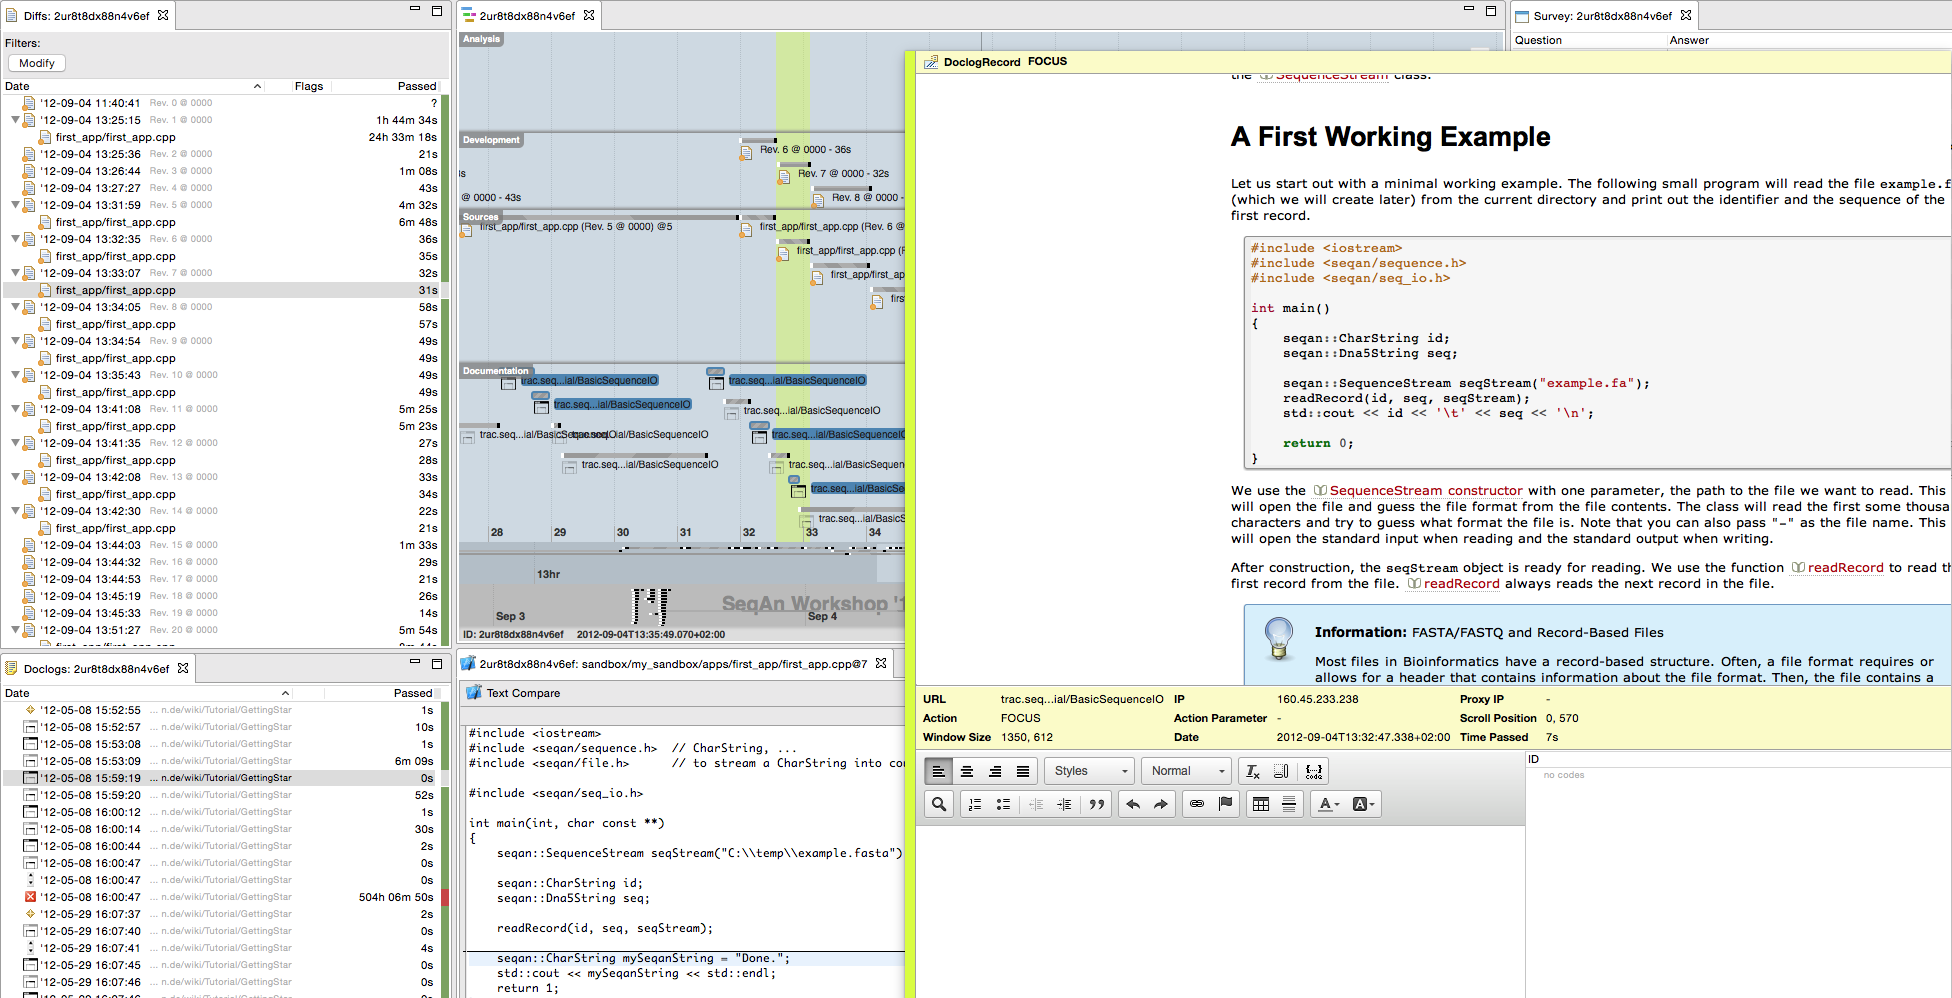
\includegraphics[width=1.0\linewidth]{Figures/AnalysisDoclog.png}
  \caption[Beispielhafte Doclog-Datei]{Dieser \gls{apiua}-Bildschirmausschnitt zeigt den Probanden \texttt{2ur8t8dx88n4v6ef}. Die Beschreibung des linken Bildbereichs kann \autoref{fig:AnalysisDiff} entnommen werden. Der blaue Bereich in der Mitte zeigt einen Abschnitt der Zeitleiste, auf der sich sämtliche Datenpunkte zum Probanden befinden. In Neon ist die Zeitspanne hervorgehoben, die zwischen dem vergangenen und dem aktuellen Kompilierversuch liegt. In der rechten Hälfte ist ein schwebender Dialog dargestellt, der Informationen zu dem Element darstellt, über dem gerade die Maus schwebt. Konkret handelt es sich um einen Doclog-Eintrag bestehend aus dem Screenshot, darunter den Metainformationen und der (leeren) Memo.}
  \label{fig:AnalysisDoclog}
\end{figure}



\subsection{Herausforderungen für ein GTM-Datenanalysewerkzeug}

Die beiden Beispiele sollten zeigen, dass \begin{enumerate}
\itemsep1pt\parskip0pt\parsep0pt
  \item hochstrukturierte Daten viele Informationen enthalten,
  \item die teilweise nur sehr aufwändig und
  \item fehleranfällig extrahiert werden können und
  \item damit potentiell die Sorgfalt bei der Anwendung der \gls{gtm} schmälert.
\end{enumerate}

Die Aufgabe eines \gls{gtm}-Datenanalysewerkzeugs darf also nicht nur darin bestehen, die Analyse technisch irgendwie zu ermöglichen. Sie besteht auch darin, zeitraubende und fehlerträchtige Routinearbeiten adäquat zu automatisieren und die Phasen und Praktiken der \gls{gtm} reibungslos zu erlauben. Die durch die \gls{gtm} ohnehin schon stark geforderte Sorgfalt und Disziplin des Forschers, dürfen durch das Datenanalysewerkzeug nicht unnötig strapaziert werden, da sonst die Qualität der generierten \gls{gt} gefährdet wäre.

Als Forscher, der sich selbst in die \gls{gtm} einarbeitete, sogar das für die eigene Datenanalyse zugehörige Analysewerkzeug selbst entwickelte und im ständigen Austausch mit seiner \gls{gtm}-affinen Forschungsgruppe\footnote{Allein diese Ausrichtung scheint äußerst selten zu sein. Zumindest wenn man sich eine Stichprobe der in führenden Softwaretechnik-Zeitschriften der Jahre 1995-1999 veröffentlichten Artikel ansieht: Demnach wurde die \gls{gtm} in weniger als 1\% der Arbeiten verwendet. \citep{Glass:2002ec}} stand, konnte ich eine Reihe von, in \autoref{tab:APIUARequirements} zusammengefassten Anforderungen formulieren.

\begin{landscape}
\begin{longtable}{p{0.2\linewidth} p{0.35\linewidth} p{0.35\linewidth}}  
  \multicolumn{1}{l}{\textbf{Anforderung}} & \multicolumn{1}{l}{\textbf{Beschreibung}} & \multicolumn{1}{l}{\textbf{Erfüllung durch \gls{apiua}}} \\ \hline 
  \endfirsthead

  \multicolumn{3}{c}{\tablename\ \thetable{} -- \textit{Fortsetzung}} \\
  \multicolumn{1}{l}{\textbf{Anforderung}} & \multicolumn{1}{l}{\textbf{Beschreibung}} & \multicolumn{1}{l}{\textbf{Erfüllung durch \gls{apiua}}} \\ \hline 
  \endhead

  \\
  \multicolumn{3}{r}{\textit{Fortsetzung auf nächster Seite}} \\
  \endfoot

  \caption{Anforderungen an \gls{gtm}-Datenanalysewerkzeuge}
  \label{tab:APIUARequirements} \\
  \endlastfoot

  Große Datenmengen &
  Die Verarbeitung von mehreren Gigabyte Datenmaterial muss unterstützt sein. &
  Auf einem durchschnittlichen Computer konnten 24GB Datenmaterial verarbeitet werden. \\
  
  Datenformate &
  Videos, Audioaufnahmen, Textdokumente, aber auch etablierte Datenaustauschformate wie XML und JSON müssen unterstützt werden. Die unterstützten Datenformate müssen erweiterbar sein. &
  Unterstützt werden lediglich die im Rahmen dieser Arbeit erfassten Datenformate. Ein \gls{plugin}-Mechanismus erlaubt die Erweiterung um beliebige weitere Datenformate (siehe \autoref{fig:apiua-plugins}). \\
  
  Offenes Kodieren &
  Die Phase des offenen Kodierens muss optimal (Kategorien, Eigenschaften, etc.) unterstützt werden. &
  Offenes Kodieren wird umfänglich unterstützt (siehe \autoref{fig:apiua-opencoding-cd}). Kategorien werden in Form von Kode-Hierarchien ermöglicht (siehe \autoref{fig:apiua-codes}). Eigenschaften werden auf Kode-Ebene definiert; entsprechende Wertebelegungen auf Kodeinstanz-Ebene erlaubt (siehe \autoref{fig:apiua-properties}). \\
  
  Axiales Kodieren &
  Die Phase des axialen Kodierens muss optimal (Relationen, etc.) unterstützt werden. Es muss Funktionen geben, die dabei helfen, \glspl{acm} zu abstrahieren. &
  Axiales Kodieren wird umfänglich unterstützt. Relationen werden auf Kode-Ebene definiert und können verankert werden. Aus den vorhandenen Relationen können automatisch \glspl{ac} und \glspl{acm} erzeugt werden (siehe \autoref{fig:apiua-axialcoding}). Abstrahierungsfunktionen existieren rudimentär in Form fest implementierter Interferenzregeln. \\
  
  Selektives Kodieren &
  Die Phase des selektiven Kodierens muss stark unterstützt werden. Dazu werden Funktionen benötigt, welche die eine weiter gehende Abstraktion / Generalisierung von Kodes, Relationen und schließlich von \glslink{acm}{axialen Kodiermodellen} erlauben. &
  Selektives Kodieren wird teilweise durch \gls{apiua}s Interferenzmöglichkeiten und Verallgemeinerung- und Zusammenfassungsmöglichkeiten von Relationen unterstützt. \\
  
  Implizites Wissen &
  In den von dem Anwender gefunden Verankerungen verbirgt sich in manchen Fällen implizites Wissen. Das Werkzeug sollte derartiges Wissen sichtbar machen. Weitere Details siehe weiter unten. &
  Implizite Verankerungen und Relationen werden sichtbar gemacht. \\
  
  Vorwissen &
  Es muss die Möglichkeit geben Verankerungen, die auf Vorwissen des Forschers beruhen, vorzunehmen. &
  Vorwissen kann durch die Verwendung von \url{bibtex:}- und \url{file:}-\acrshort{uri}s verankert werden. \\
  
  Umstrukturierungs-\\operationen\footnote{Auch wenn man verführt ist, die Bezeichnung \textit{Refactoring} zu verwenden, wäre die von \cite{Fowler:424198} formulierte Anforderung verletzt, dass die Semantik bei einer derartigen Operation nicht verändert wird. Eine kanonische Übertragung dieser Eigenschaft auf Theorien ist nicht möglich, da die Grenzen einer Theorie nicht hinreichend scharf sind. Während man sich noch streiten kann, ob einfache Operationen, wie eine Kode-Umbenennung, bereits die Semantik einer Theorie ändern, ist die Frage bei komplexeren Operationen wie die Verallgemeinerung von Relationen eindeutig mit ``ja'' zu beantworten.} &
  Es muss Möglichkeiten geben, Änderungen an der Modellierung vorzunehmen, die der \gls{gt} zu Grunde liegt. Beispiele sind Kode-Umbenennung, Verallgemeinerung oder Spezialisierung von Relationen, Verschieben von Kode-Eigenschaften und Zusammenfassung oder Auftrennen von Kodes. &
  Einige Strukturänderungsoperationen werden unterstützt. Dazu gehören einfache Operationen wie die Umordnung des Kode-Baumes und die Verallgemeinerungen bzw. Zusammenfassung von Relationen (siehe \fref{fig:apiua-feature-generalization-relation}). Außerdem können während der Zuweisung von Phänomenen zu Kodes in einem speziellen Dialog (siehe \fref{fig:apiua-feature-properties-assignment}) direkt Eigenschaftswerte zugewiesen werden. \\
  
  Weitergehende Analysefunktionen &
  Beispielsweise könnte eine Funktion, die anzeigt, welche Kodes in welchen Datenquellen/-erhebungen verankert sind, bei der Bewertung der Frage helfen, ob und in welche Richtung eine weitere Datenerhebung gehen kann/soll. Diese Funktion würde also den Forscher beim \textit{theoretischen Sampling} unterstützen. &
  Weitere Analysefunktionen wurden aus zeitlichen Gründen nicht implementiert. \\
  
  Interoperabilität &
  Die Forschungsergebnisse müssen in einem Format gespeichert werden, das sich zur Weiterverarbeitung durch dritte Programme eignet. Darüber hinaus erlaubt die Verwendung standardisierter Datenformate die Bereitstellung der Forschungsdaten im Rahmen von \textit{Open Science} --- also in diesem Fall, dem freien Zugang zu wissenschaftlichen Ergebnissen. &
  Die Forschungsergebnisse werden in XML abgelegt. Memos werden in Form von HTML-Dateien abgelegt, deren Name der \gls{uri} des beschriebenen Datenpunktes entspricht. \Glspl{acm} liegen in Form von JSON-Dateien vor. Datenpunkte werden innerhalb der HTML- und JSON-Dateien einheitlich mit deren \gls{uri} referenziert, was jede Möglichkeit von technischer Datenredundanz ausschließt.  \\
  
  Usability &
  Die Usability des Werkzeugs selbst muss hoch sein, um die Qualität der erarbeiteten \gls{gt} nicht zu schmälern. &
  Der Zustand der Arbeitsumgebung wird vollständig gesichert, d.h. die Anordnung der verschiedenen Bereiche, deren Anzeigeoptionen, deren Inhalt und viele weitere Informationen, wie zuletzt verwendete Kodes, werden nach einem Neustart der Anwendung wiederhergestellt. Zur Erfüllung einer Aufgabe werden verschiedene Möglichkeiten angeboten. Zuletzt verwendete Elemente (Kodes, Phänomene, etc.) werden in einer Historie festgehalten. Kodes werden automatisch mit sinnvollen Farben versehen. \\
  
  Plattformabhängigkeit & --- & \gls{apiua} ist lauffähig unter Windows, Mac OS und Linux.\\
\end{longtable}
\end{landscape}

\begin{figure}
  \centering
    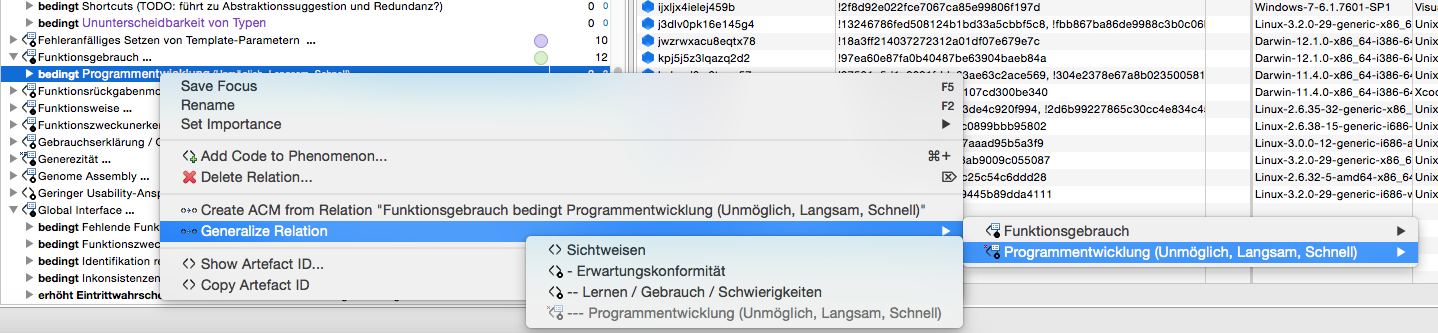
\includegraphics[width=1.0\linewidth]{Figures/apiua/feature-generalization-relation.png}
  \caption[APIUA: Verallgemeinerung von Relationen]{Dieser Screenshot von \gls{apiua} zeigt das die Möglichkeit zur Verallgemeinerung von Relationen.}
  \label{fig:apiua-feature-generalization-relation}
\end{figure}

\begin{figure}
  \centering
    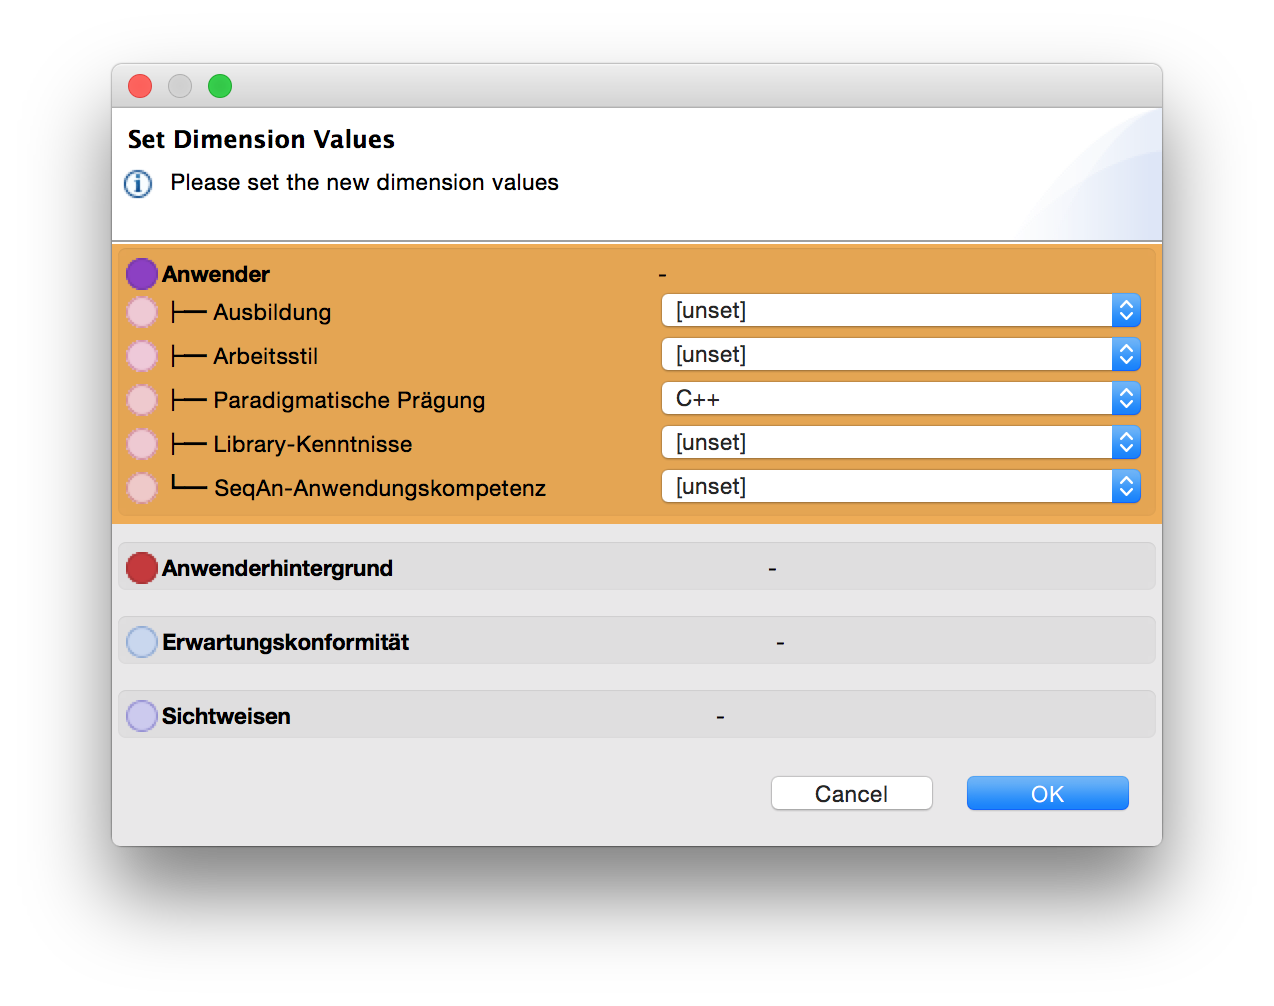
\includegraphics[width=0.5\linewidth]{Figures/apiua/feature-properties-assignment.png}
  \caption[APIUA: Wertezuweisung bei Umstrukturierungen]{Dieser Screenshot von \gls{apiua} zeigt den Dialog zur Zuweisung von Eigenschaftswerten bei Umstrukturierungen.}
  \label{fig:apiua-feature-properties-assignment}
\end{figure}

Im \sref{sec:gtm-implementation} auf Seite \pageref{sec:gtm-implementation} gehe ich genauer auf einige der Anforderungen und ihrer Erfüllung durch \gls{apiua} ein. Der folgende Abschnitt soll zunächst den groben technischen Aufbau von \gls{apiua} vorstellen.

\begin{figure}
  \centering
    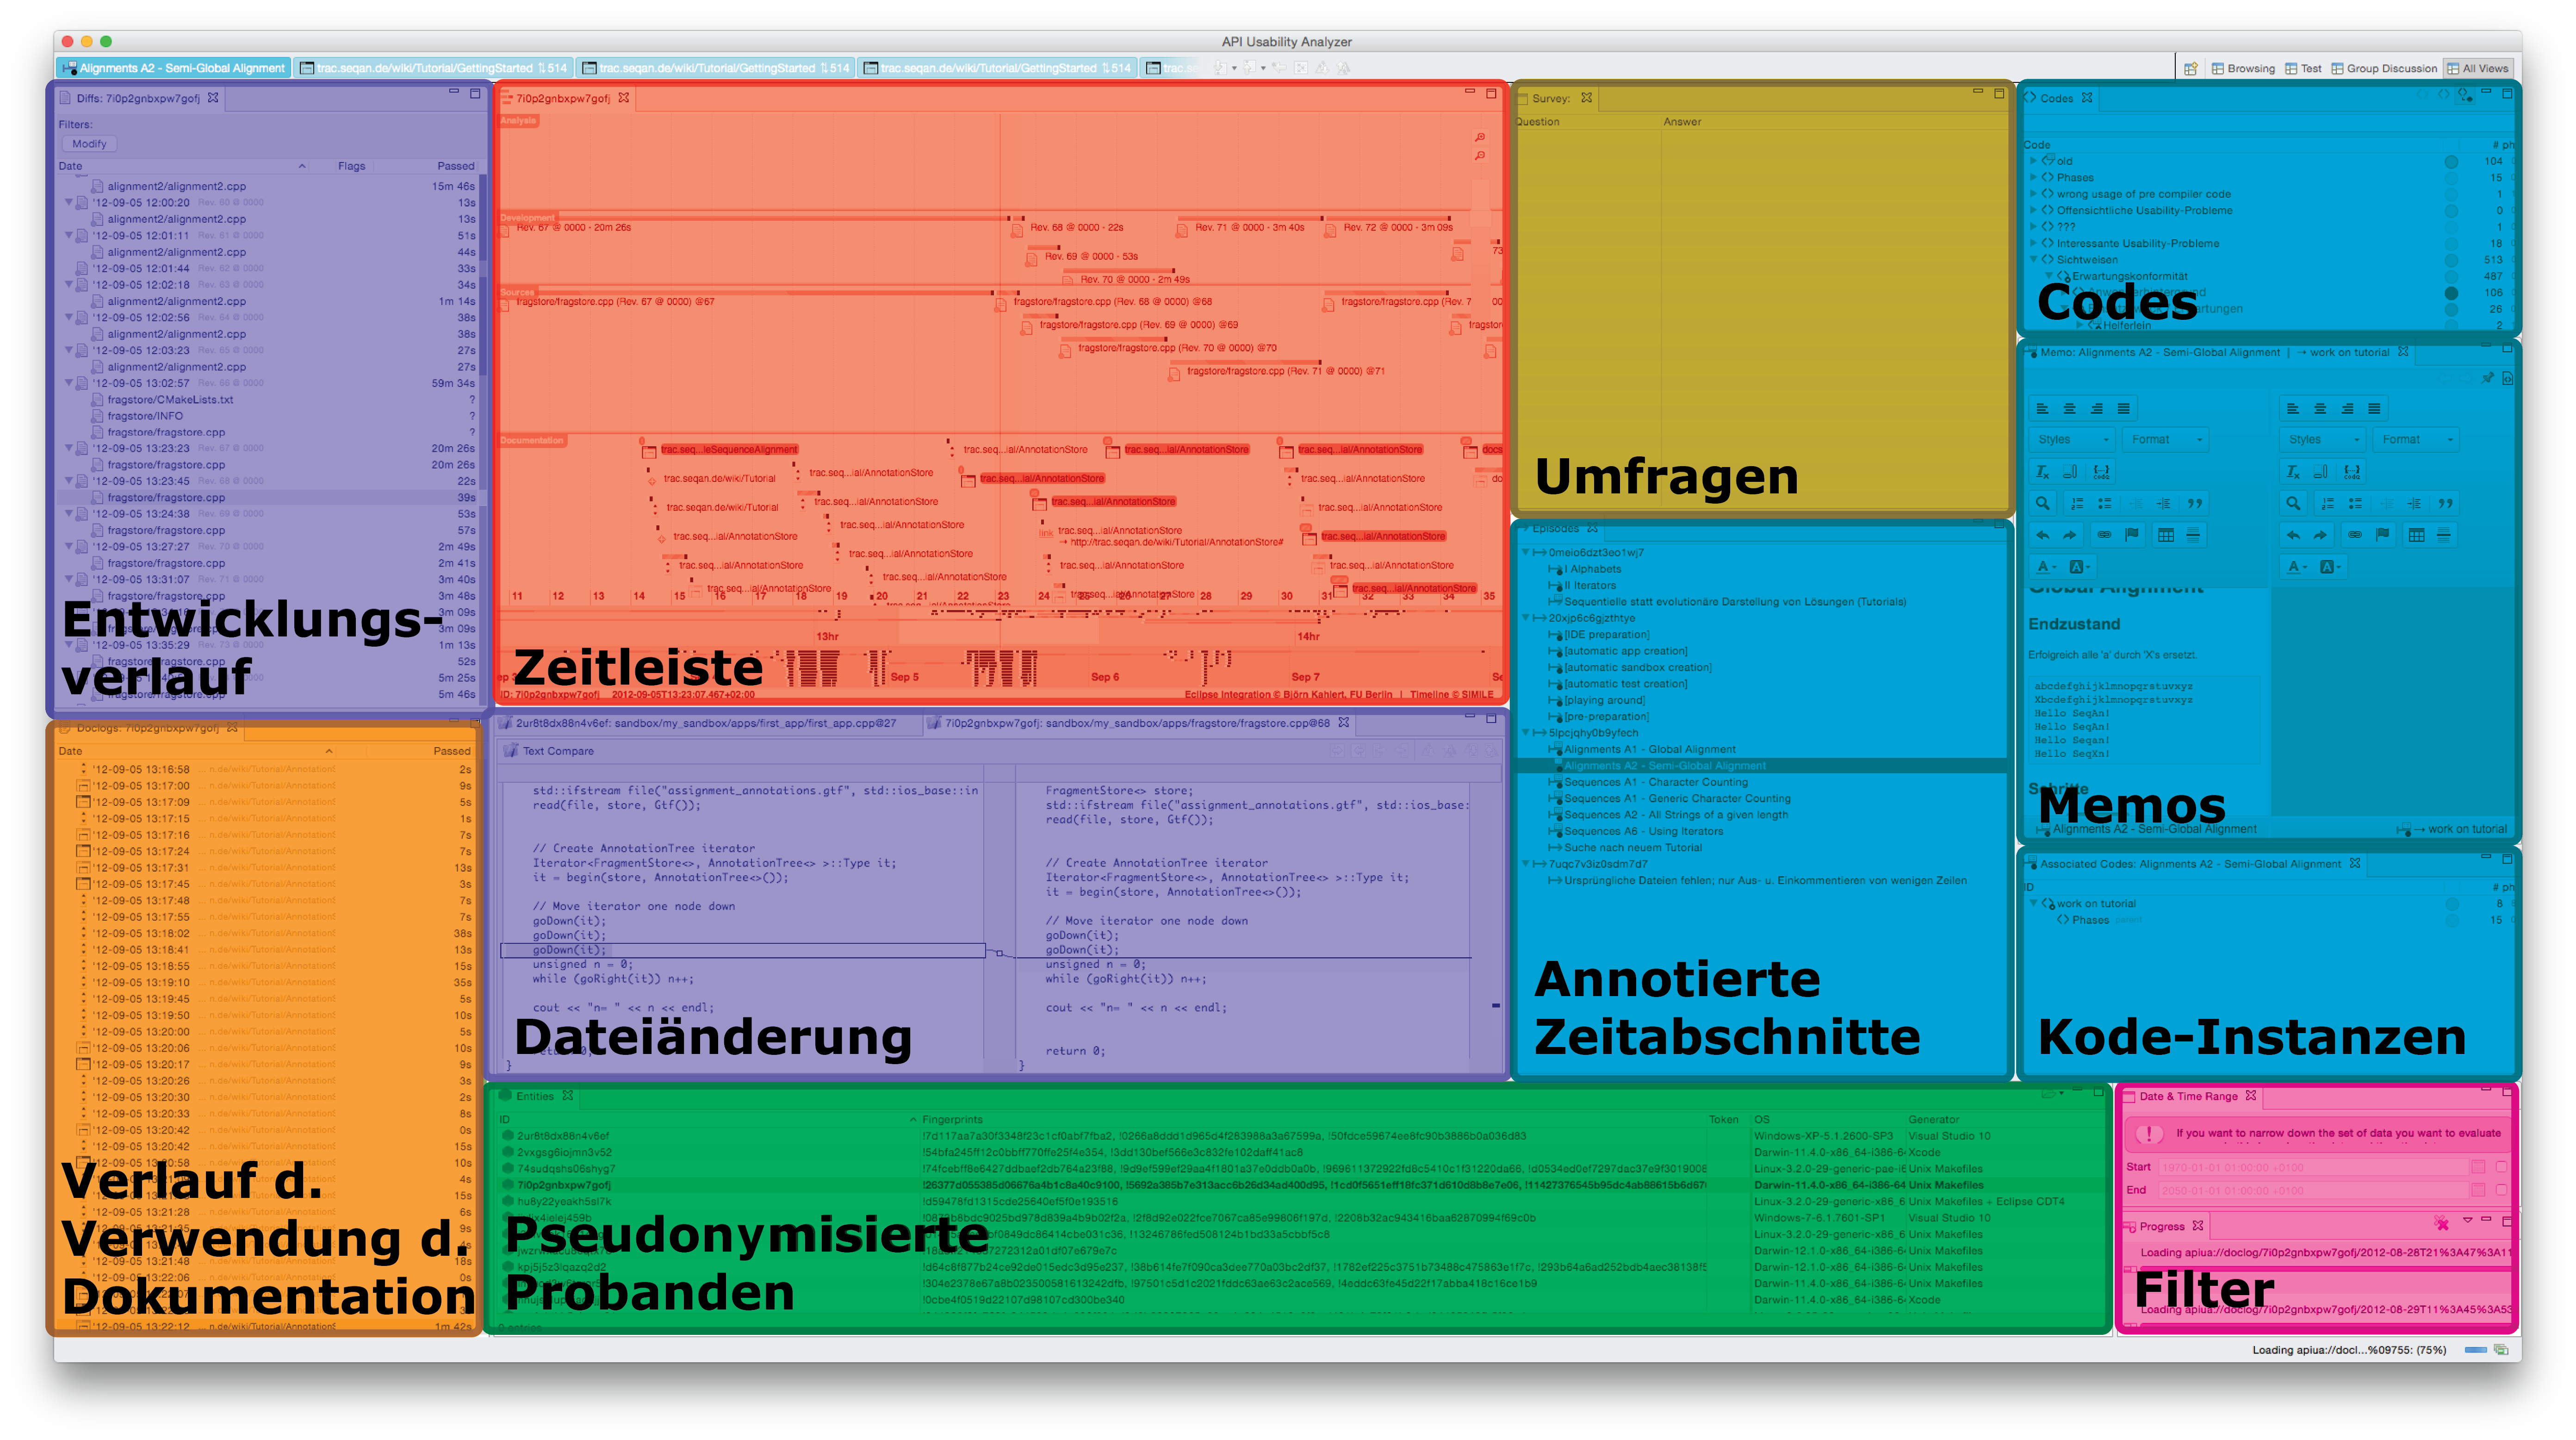
\includegraphics[width=1.0\linewidth]{Figures/apiua/plugins.png}
  \caption[APIUA: Architektur --- Plugins]{Dieser Screenshot von \gls{apiua} in der Perspektive für offenes Kodieren zeigt die von den verschiedenen \glspl{plugin} der Schicht 3 beigesteuerten Eclipse-Views.\\
  V.\,l.\,n.\,r.: Violett: Diff-\gls{plugin}; Rot: Timeline-\gls{plugin}; Gelb: Stats-\gls{plugin}; Blau: GTM-\gls{plugin}; Orange: Doclog-\gls{plugin}; Grün: Entity-\gls{plugin}; Pink: Core-\gls{plugin}}
  \label{fig:apiua-plugins}
\end{figure}

\begin{figure}
  \centering
    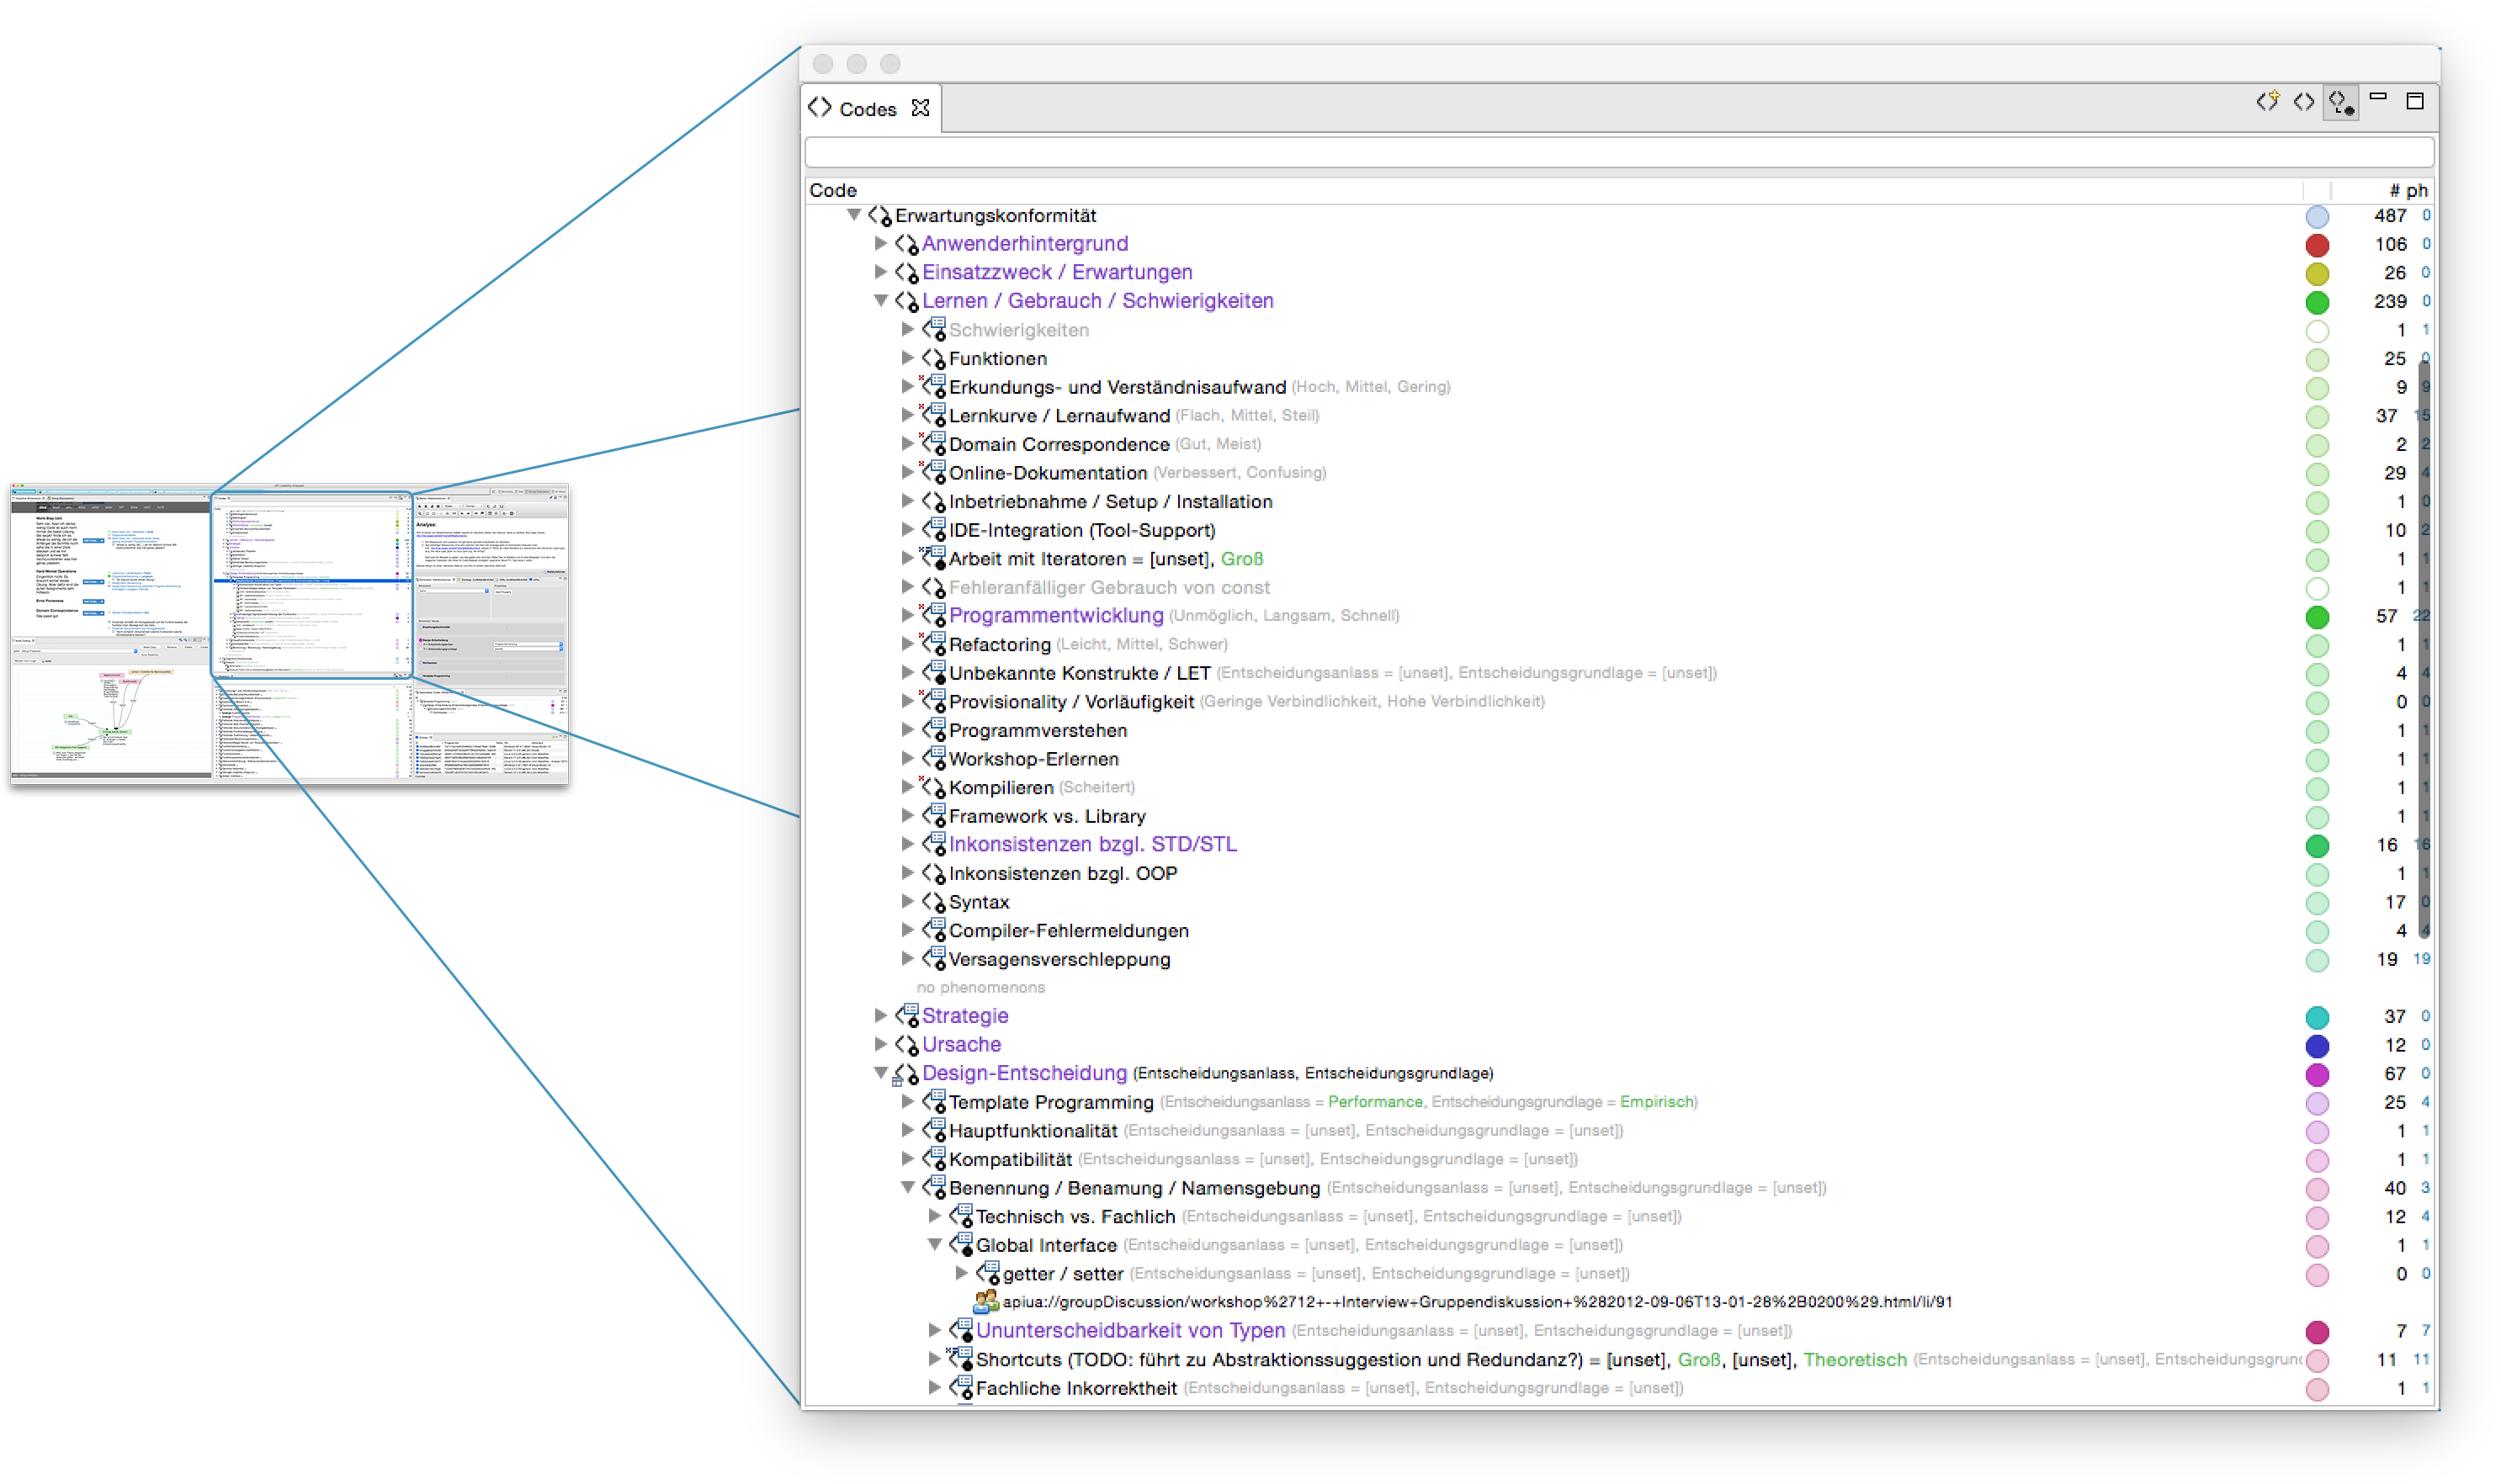
\includegraphics[width=1.0\linewidth]{Figures/apiua/codes.png}
  \caption[APIUA: Kode-Ansicht]{Dieser Screenshot von \gls{apiua} zeigt das Eclipse-View ``Codes'', das alle verankerten Kodes darstellt.}
  \label{fig:apiua-codes}
\end{figure}

\begin{figure}
  \centering
    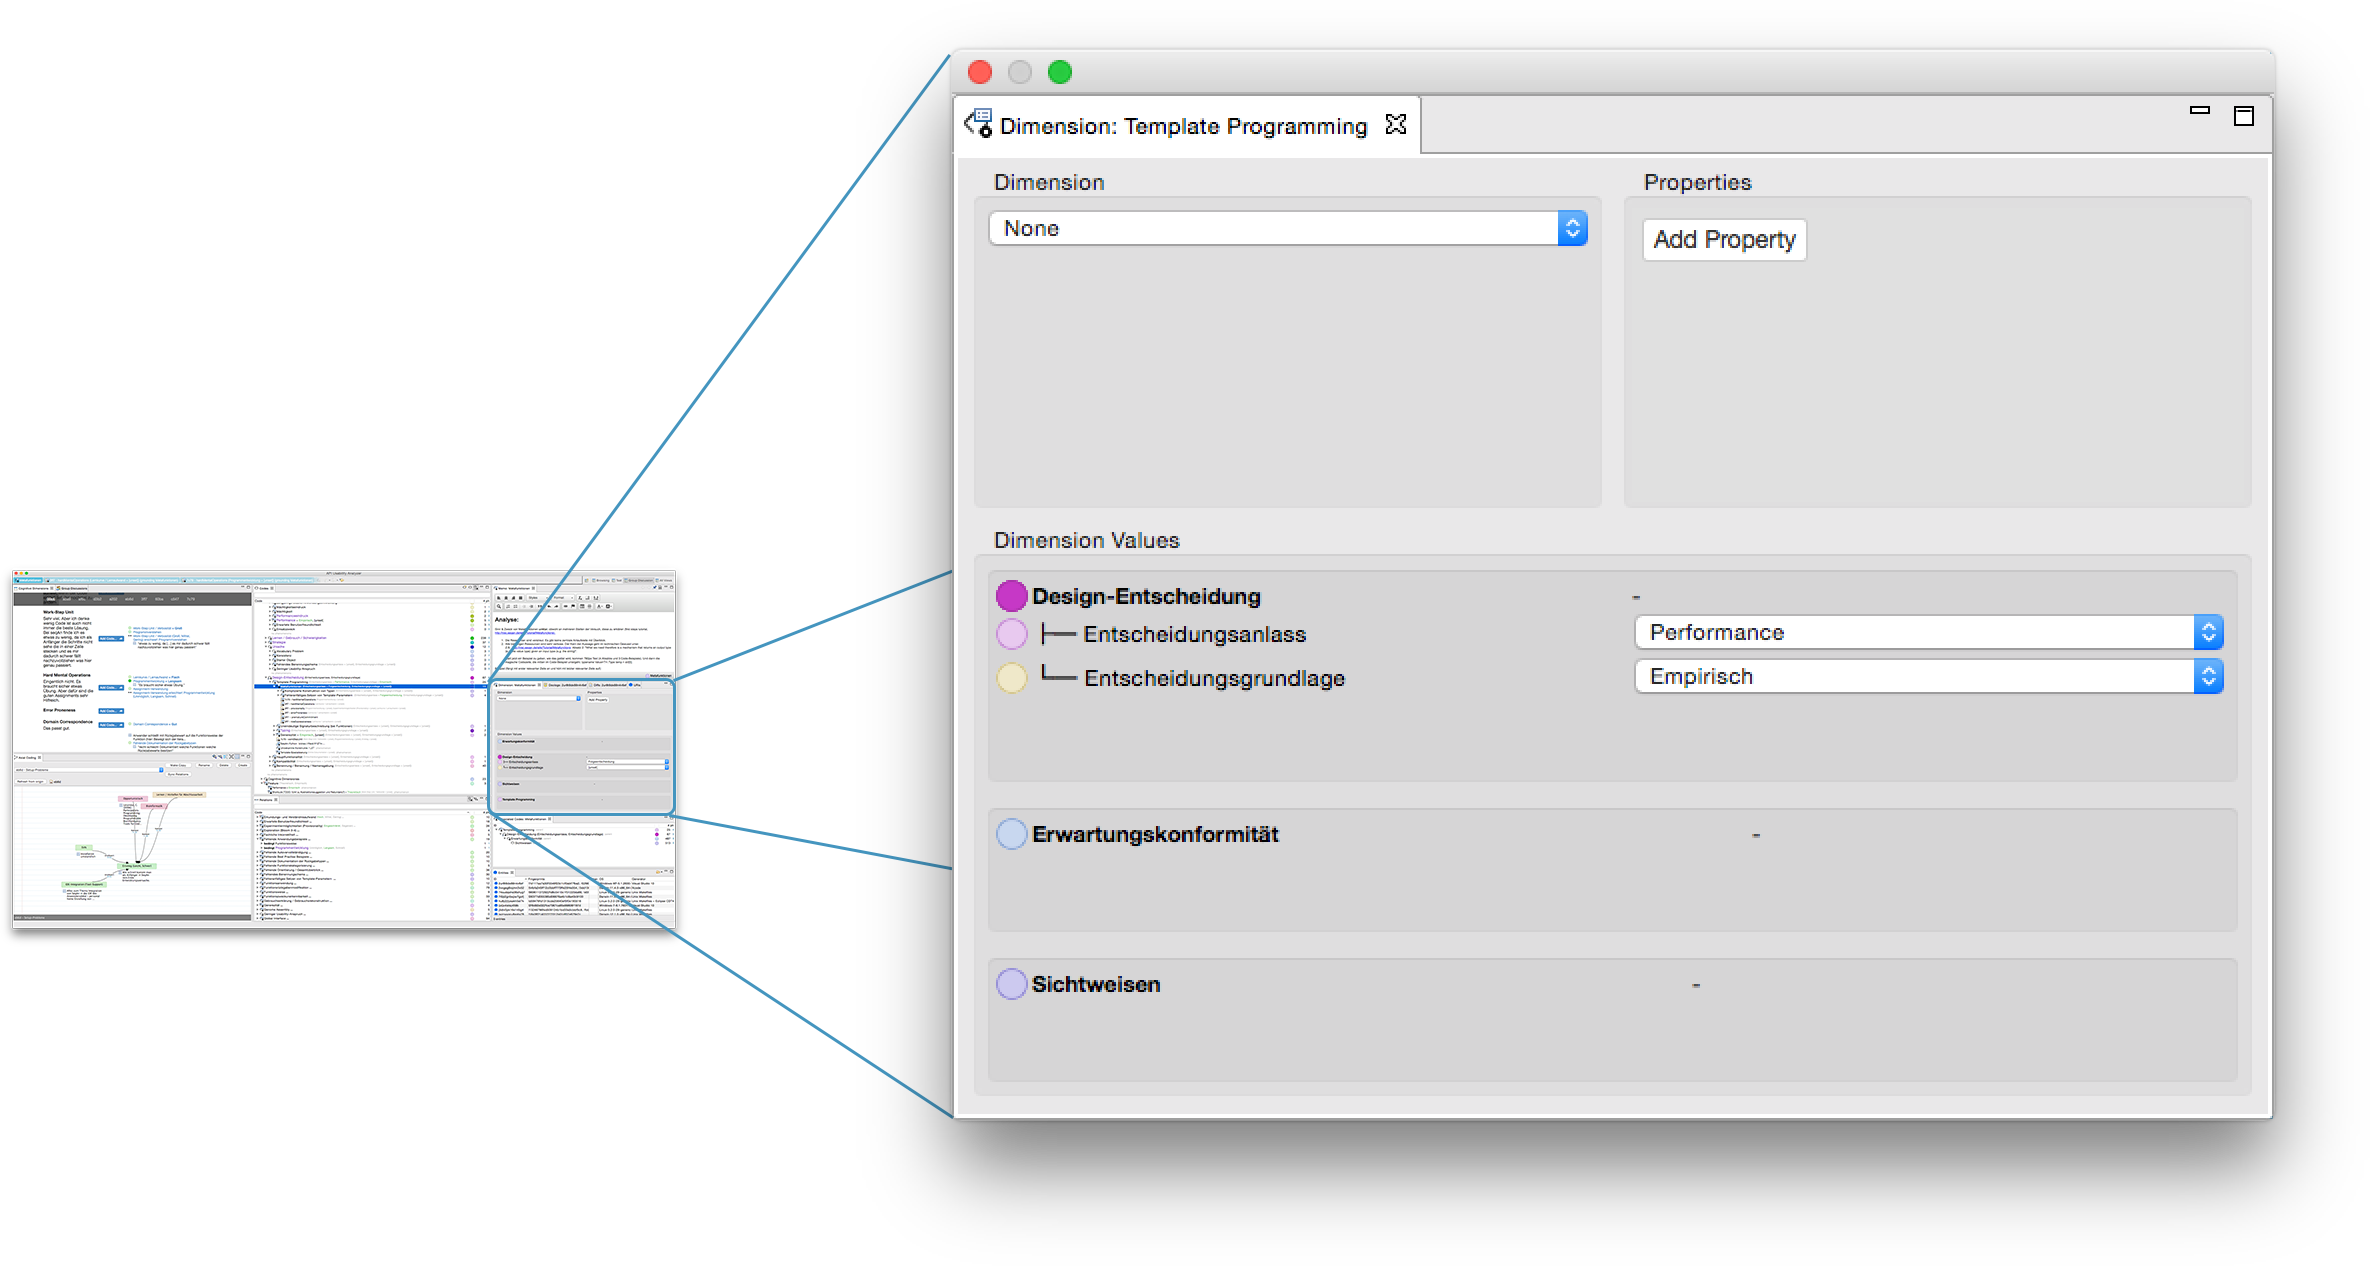
\includegraphics[width=1.0\linewidth]{Figures/apiua/properties.png}
  \caption[APIUA: Eigenschaften-Ansicht]{Dieser Screenshot von \gls{apiua} zeigt das Eclipse-View ``Dimension'', das die Dimension, alle Eigenschaften und Wertebelegungen für das aktuell selektierte Element darstellt.}
  \label{fig:apiua-properties}
\end{figure}



\subsection{Entwurf}

In diesem Abschnitt werden die wichtigsten \gls{apiua}-Entwurfsentscheidungen vorgestellt. Die vollständigen Quellen von \gls{apiua} sind unter \gls{github}\footnote{\url{https://github.com}} veröffentlicht und werden dort gepflegt.

\Gls{apiua} basiert auf der \textit{\gls{rcp}}\footnote{\url{http://wiki.eclipse.org/index.php/Rich\_Client\_Platform}} (Version 3), die wiederum die Grundlage für die bekannte Entwicklungsumgebung \textit{\gls{eclipse}} darstellt.

Architektonisch verwendet \gls{apiua} einen Hybrid aus einer serviceorientierten und einer schichtenbasierten Architektur (siehe \autoref{fig:Architecture}).

\begin{figure}
  \centering
    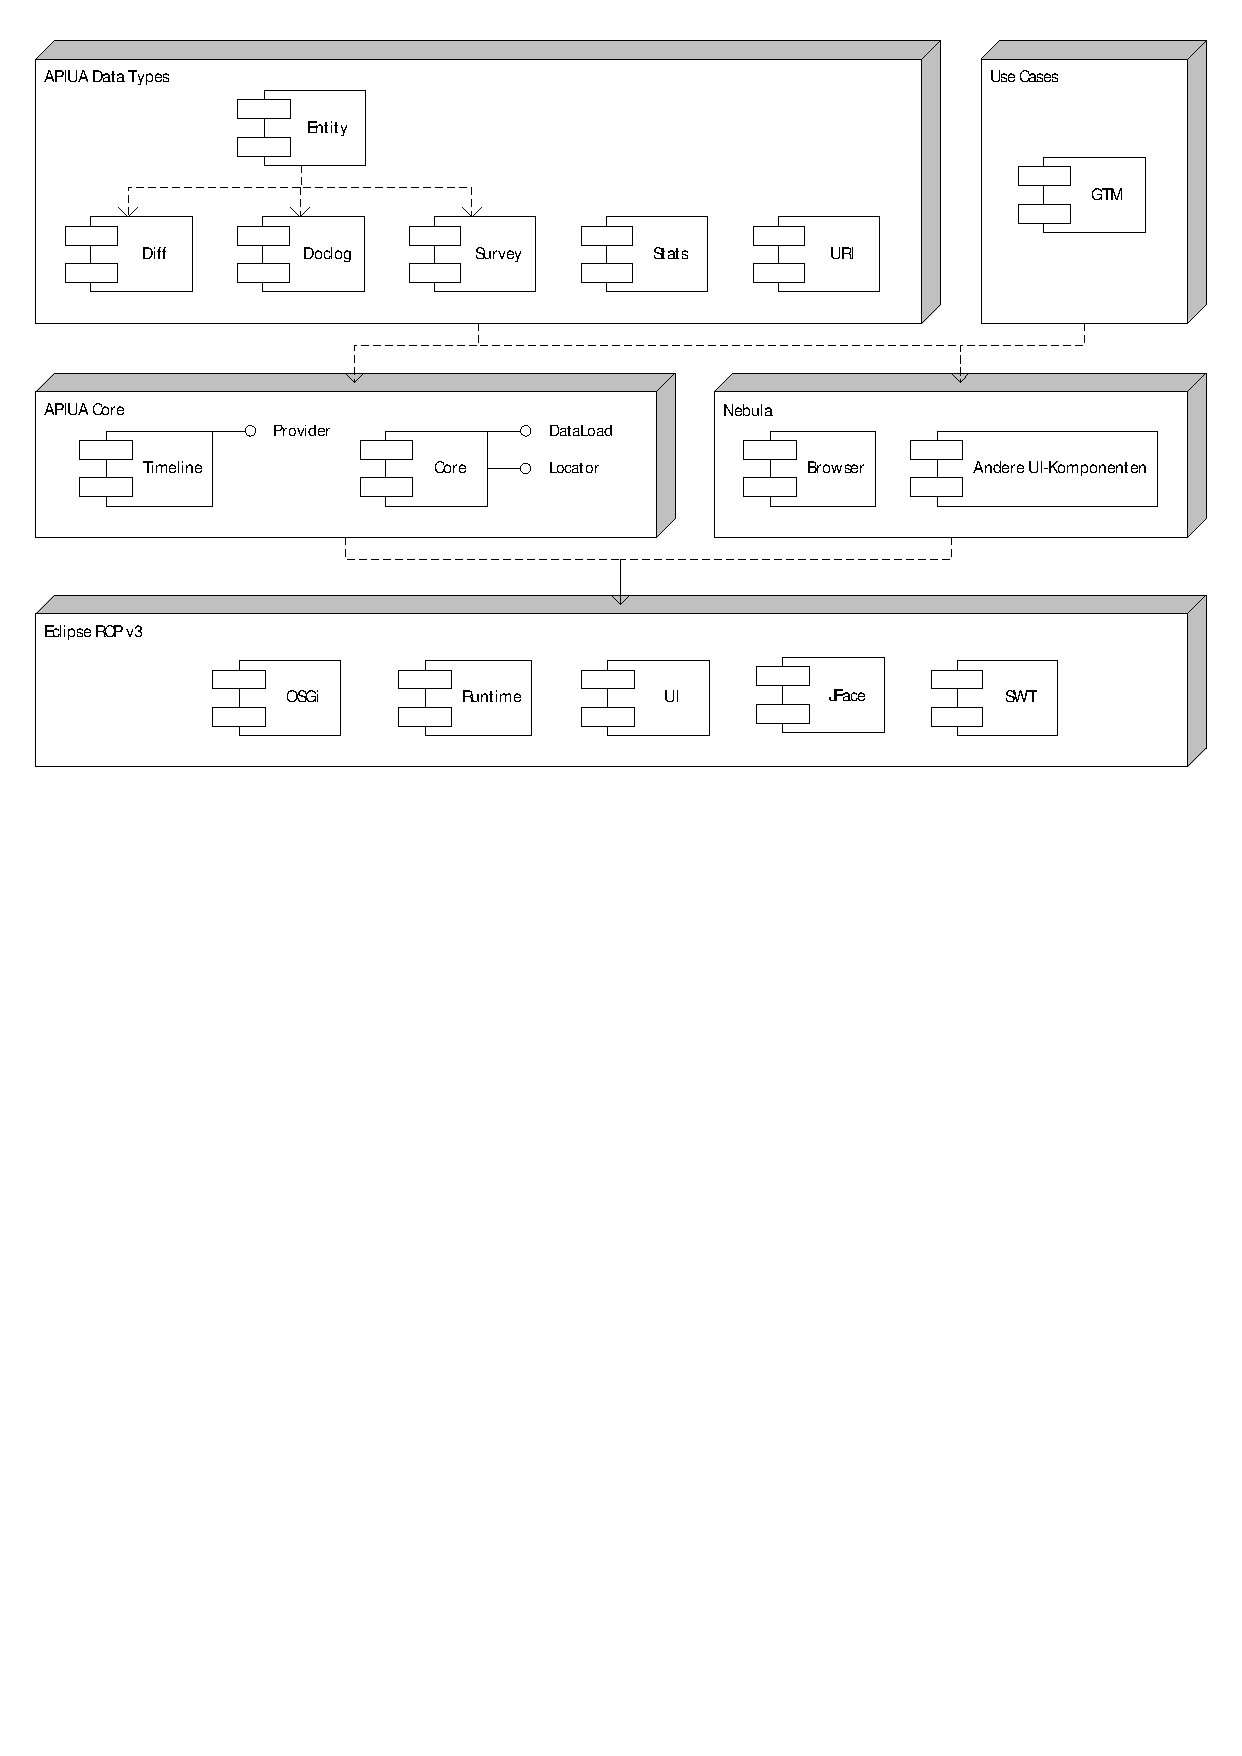
\includegraphics[width=1.0\linewidth,trim=0cm 16.5cm 0cm 0cm]{Figures/architecture.pdf}
  \caption[APIUA: Architektur --- Schichten]{Dieses UML-Diagramm beschreibt die Architektur von \gls{apiua}. Sie besteht aus den folgenden drei Schichten: \gls{rcp}-Schicht, Infrastrukturerweiterungsschicht (Core und Nebula),  Komponentenschicht (Data Types, Use Cases).}
  \label{fig:Architecture}
\end{figure}


\subsubsection{Schicht 1: Eclipse Rich Client Platform}

Die unterste Schicht bildet die \gls{rcp}-Schicht und stellt das Fundament von \gls{apiua} dar.

Die Komponenten \textit{\acrshort{osgi}} und \textit{Runtime} stellen den, von \gls{eclipse} bekannten Plugin-Mechanismus bereit und erlauben es, die Kopplung zwischen Modulen (hier: \gls{plugin}s) erheblich zu verringern. Die \textit{\gls{swt}}-Komponente erlaubt den plattformübergreifend einheitlichen Zugriff auf plattformabhängige UI-Elemente. \textit{JFace} und \textit{UI} ermöglichen die, von \gls{eclipse} bekannte, Organisation des Anwendungsfensters mit Hilfe von Perspektiven, Editoren und Ansichten (engl. \textit{views}).


\subsubsection{Schicht 2: Infrastrukturerweiterung}

Die zweite Schicht besteht aus zwei Teilen, die die \gls{rcp}-Schicht um weitere Infrastruktur-Funktionalitäten erweitert.

Den ersten Teil stellt das \textit{Nebula}-\gls{plugin} dar, das ich im Rahmen meiner Masterarbeit entwickelt \citep{Kahlert:2011wr} habe. Es stellt wiederverwendbare \gls{swt}-Komponenten bereit, die nach meiner Ansicht Bestandteil des \gls{swt}-\gls{plugin}s selbst hätten sein sollen. Die Komponenten wurden im Rahmen dieser Arbeit von mir um eine Browser-Komponente ergänzt, welche ausführlich im \aref{sec:browser} erläutert wird. Kurzfassung: Viele Teile der \gls{ui} von \gls{apiua} sind programmatisch sehr anspruchsvoll. Um den Entwicklungsaufwand gering zu halten, traf ich die Entscheidung, die umfangreiche Funktionalität moderner Webbrowser wiederzuverwenden und \gls{ui}-Elemente basierend auf den Websprachen HTML, CSS/Less\footnote{Less (\url{http://lesscss.org}) stellt gemeinsam mit Sass (\url{http://sass-lang.com}) die populärste Spracherweiterung für CSS dar. Sie erlauben beispielsweise die Verwendung von Schleifen und Variablen. Die gleichnamigen Präprozessoren sind dafür zuständig, \texttt{.less}- bzw. \texttt{.sass}-Dateien nach CSS zu kompilieren.} und JavaScript zu entwickeln. Der \textit{Nebula}-Browser ist dafür zuständig, die so entwickelten \gls{ui}-Elemente darzustellen.

Der zweite Teil ist das \textit{Core}-\gls{plugin}. In Form von Diensten stellt es Funktionalität zur Datenorganisation bereit. Dazu gehören die Datenpersistierung, sowie die Möglichkeit, Forschungsdaten zu laden. Erweiterungspunkte (in \gls{eclipse} heißen sie \textit{extension points}) und Dienste machen das \textit{Core}-\gls{plugin} zu einem Bussystem, über das \glspl{plugin} anderen \glspl{plugin} (insbesondere denen der Schicht 3) Daten zur Verfügung stellen können. Produzenten und Konsumenten werden dadurch entkoppelt. Weitere Details zu den bereitgestellten Diensten werden im \aref{sec:services} beschrieben.

Im \textit{Core}-\gls{plugin} manifestiert sich außerdem eine grundlegende Entwurfsentscheidung. Sie besteht darin, jede Art von Datum mittels eines \gls{uri} adressierbar zu machen. Nicht nur die Datenhaltung sondern alle Komponenten verwenden \gls{uri}s zum Lokalisieren von Daten. Die Größe der im Rahmen dieser Arbeit erfassten Daten beträgt mehr als 24GB\footnote{Diese Angabe bezieht sich auf die expandierten Daten. Das heißt, die Daten wurden so aufbereitet, dass sie effizient lesend verarbeitet werden können. Zur Aufbereitung gehören unter anderem die Erstellung von Screenshots und die Berechnung der effektiven Quellcode-Dateien auf Grundlage vorliegender Diff-Dateien.}. Diese Datenmenge kann nicht problemlos bei jedem Programmstart in den Arbeitsspeicher geladen werden. Darum stellt dieses Plugin den \textit{LocatorService} bereit. Dieser erlaubt den intelligenten und speicherschonenden Zugriff\footnote{Dieser Dienst setzt einen Cache ein, der Einträge auf Basis von Zugriffshäufigkeiten verdrängt.} auf Datenobjekte --- unabhängig davon, ob sie gerade geladen sind oder nicht.

Mit wenigen Ausnahmen haben \gls{uri}s folgenden Aufbau:

\begin{center}\texttt{apiua://\textit{datatype}/\textit{id}/\textit{detail}}\end{center}

\bigskip

\begin{description}
	\item[datatype] bezeichnet den Datentyp bzw. das Datenformat. Beispiele sind \textit{diff} und \textit{entity}.
	\item[id] bezeichnet einen Identifikator. Beispiel: 2ur8t8dx88n4v6ef
	\item[detail] erlaubt eine feingliedrigere Lokalisierung. Dieser Teil ist sehr von dem Datentyp abhängig.
\end{description}

\textbf{Beispiel 1:}\\\texttt{apiua://code/526} verweist auf einen Kode mit der ID \texttt{526}.

\textbf{Beispiel 2:}\\\texttt{apiua://diff/2ur8t8dx88n4v6ef/5/\%2Fmy\_sandbox/\%2Ffirst\_app.cpp} beschreibt die von Proband \texttt{2ur8t8dx88n4v6ef} in der 6. Iteration editierte Datei \texttt{first\_app.cpp}, die sich im Ordner \texttt{my\_sandbox} befindet.

Auch wenn ich diese Funktion nicht implementiert habe, könnte man, für das sich im Einsatz befindliche Betriebssystem, einen \textit{url scheme handler} programmieren, der \glspl{uri} mit dem Schema \texttt{apiua} öffnet, um die Interoperabilität zwischen \gls{apiua} und Drittsoftware zu verbessern.




\subsubsection{Schicht 3: Komponentenschicht}
\label{sec:schicht3}

Diese Schicht besteht wiederum aus zwei Teilen, die die für den Anwender sichtbare Funktionalität implementieren.

Der erste Teil wird als \textit{data types} bezeichnet und folgt einer Komponenten-basierten Architektur. Jede Komponente / jedes \gls{plugin} innerhalb dieses Teils
\begin{itemize}
	\item ist ausschließlich abhängig von unteren Architekturschichten\footnote{Die Komponente \textit{Entity} bildet eine Ausnahme, denn sie synthetisiert die geladenen Daten anderer Komponenten (siehe \sref{sec:datenerhebung}).},
	\item stellt einen bestimmten Datentyp/-format über den \textit{Core}-\gls{plugin}-Bus allen Konsumenten bereit,
	\item kann Daten dieses Datentyps/-formats lesen,
	\item stellt \gls{eclipse}-Views bereit, die die geladenen Daten visualisieren (vgl. \autoref{fig:apiua-plugins}) und
	\item stellt Visualisierungsinformationen (Bezeichnung, Ikone, Meta- und Detailinformationen) für Daten des Datentyps/-formats über den \textit{Core}-\gls{plugin}-Bus bereit.
\end{itemize}

Die Anforderungen werden, wie bereits weiter oben beschrieben, ausschließlich über \gls{plugin}-Erweiterungen und \textit{Core}-\gls{plugin}-Dienste realisiert. Die Architektur und die damit einhergehende geringe Kopplung machen das Werkzeug \gls{apiua} besonders wart- und erweiterbar. Unterstützung für weitere Datentypen/-formate kann problemlos in Form von \gls{plugin}s geschaffen werden. 

Der zweite Teil stellt die \textit{Use Cases} (Anwendungsfälle) implementierenden Komponenten dar. Tatsächlich gibt es nur die \gls{gtm}-Komponente, die es erlaubt, Kodes, Relationen und deren Eigenschaften auf der Grundlage der, durch die Datentyp-Komponenten bereitgestellten Daten zu modellieren. Da jedes Datum eine \gls{uri} besitzt und das \textit{Core}-Plugin Visualisierungsinformationen zwischen den \gls{plugin}s vermittelt, kann auch dieses \gls{plugin} mit nur wenigen Abhängigkeiten arbeiten.
  





\subsection{Funktionsweise von APIUA und Implementierung der GTM}
\label{sec:gtm-implementation}

Ursprünglich wollte ich ein Datenanalysewerkzeug schaffen, das exakt meine Bedürfnisse erfüllt. Das bedeutet, es muss meine Interpretation der \gls{gtm} und meine speziellen Daten unterstützen. Ich habe dabei bewusst den Aufbau anderer Datenanalysewerkzeuge ignoriert, um eine möglichst hohe Spezialisierung auf meine Anforderungen zu erreichen. Umso erstaunlicher ist es, dass die Entwicklung am Ende mehr als 18 Monate ``verschlingen'' sollte und den etablierten Werkzeugen am Ende ähnlicher war, als ich erwartet hatte.

\paragraph{Terminologie}

Die terminologische Ähnlichkeit zu \textit{ATLAS.ti} zeigt \autoref{tab:terminology}. Am meisten fällt auf, dass mein verwendetes Vokabular eher technisch getrieben ist. Ein Beispiel dafür ist die Kodeinstanz, die in der \gls{gtm} als Konzeptualisierung bezeichnet wird. Als zweites Beispiel soll das \gls{gtm}-Phänomen dienen, welches in \gls{apiua} \textit{Locatable} genannt wird. Es handelt sich dabei um das Interface, das von jedem Datenformatstyp (siehe \sref{sec:schicht3}) implementiert wird und damit durch das \gls{gtm}-Plugin verarbeitet werden kann. 

  \begin{table}  	
    \begin{threeparttable}
    \begin{tabularx}{\linewidth}{X X X}
    \textbf{\gls{gtm}} & \textbf{ATLAS.ti} & \textbf{\gls{apiua}} \\
    \midrule
    Phänomen\\(\textit{Phenomenon}) & \textit{Quotation}\tnote{a} & \textit{Locatable}\tnote{b} \\
    Konzeptualisierung (\textit{Conceptualization}) & Annotation & Kodeinstanz (\textit{Code Instance}) \\
    Konzept (\textit{Concept}) & \textit{Code} & Kode (\textit{Code}) \\
    Eigenschaft (\textit{Property}) & \textit{Code} & Eigenschaft\tnote{d} (\textit{Property}) \\
    Kategorie (\textit{Category}) & \textit{Code}\tnote{c} & Kode (\textit{Code})\tnote{e} \\
    Beziehung (\textit{Relationship}) & \textit{Relationship}/\textit{Relation} & \textit{Relation} \\
    \end{tabularx}
    \begin{tablenotes}
      \item[a] In \textit{ATLAS.ti} handelt es sich um Datenausschnitte.
      \item[b] In \gls{apiua} handelt es sich um Datenausschnitte, deren Granularität ---~in Abhängigkeit vom Datentyp~--- programmatisch vorgegeben ist.
      \item[c] Technisch handelt es sich um einen dimensionalisierten Kode, der als Eigenschaft eines anderen Kodes deklariert wird.
      \item[d] In ATLAS.ti können zur Modellierung \textit{Code Families} verwendet werden.
      \item[e] In \gls{apiua} sind Kodes hierarchisch angeordnet. Eine Kategorie ist ein Kode mit Unterkodes.
    \end{tablenotes}
    \end{threeparttable}
    \caption[Gegenüberstellung von GTM-Begriffen]{Gegenüberstellung der in der \gls{gtm}, in \textit{ATLAS.ti} und in \gls{apiua} verwendeten Begriffe. Die Angaben zur \gls{gtm} und  \textit{ATLAS.ti} entstammen \cite{Salinger:2013vd}.}
    \label{tab:terminology}
  \end{table}
  
\paragraph{Organisation des Arbeitsbereichs}

In \textit{ATLAS.ti} gibt es verschiedene Ansichten, die exklusiv sind, d.h. niemals parallel geöffnet sein können. \gls{apiua} hingegen verwendet die erprobte Organisation der Benutzeroberfläche nach Perspektiven. Perspektiven können frei definiert werden. Eine Perspektive besteht aus einer frei wählbaren Anordnung gewünschter Ansichten. Perspektiven für die Phasen des offenen und axialen Kodierens sind bereits vordefiniert (siehe Abbildungen \ref{fig:apiua-opencoding-devel}, \ref{fig:apiua-opencoding-cd}, \ref{fig:apiua-opencoding-gd} und \ref{fig:apiua-axialcoding}). \fref{fig:apiua-browsing} zeigt die Perspektive für die Exploration des gesammelten Datenmaterials.





\subsubsection{Offenes Kodieren}
\label{sec:apiua-open-coding}

Das Kodieren von Datenmaterial ähnelt sich in den typischen CAQDAS-Werkzeugen und besteht im Grunde darin, einem referenzierbaren Datenausschnitt (\gls{gtm}: Phänomen) einen Kode zuzuordnen, der entweder schon existiert oder innerhalb dieses Prozesses erstellt wird. Typischerweise kommt dabei Drag'n'Drop zum Einsatz. Erstellte Kodes und annotierte Datenausschnitte (\gls{gtm}: Konzeptualisierung) werden listenartig dargestellt. Die Abbildungen \ref{fig:apiua-codes-atlas} und \ref{fig:apiua-codeinstances-atlas} zeigen, wie diese Kode-Darstellung in \gls{apiua} und \textit{ATLAS.ti} realisiert wird.

\begin{figure}
  \centering
    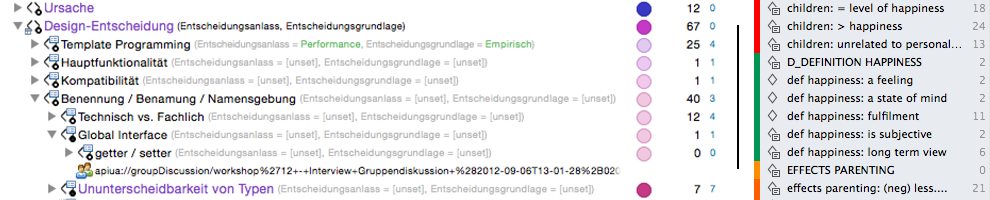
\includegraphics[width=1.0\linewidth]{Figures/apiua/codes-atlas.png}
  \caption[Vergleich APIUA und ATLAS.ti: Kode-Darstellung]{Vergleich Kode-Darstellung; links: \gls{apiua}; rechts: \textit{ATLAS.ti}}
  \label{fig:apiua-codes-atlas}
\end{figure}

\begin{figure}
  \centering
    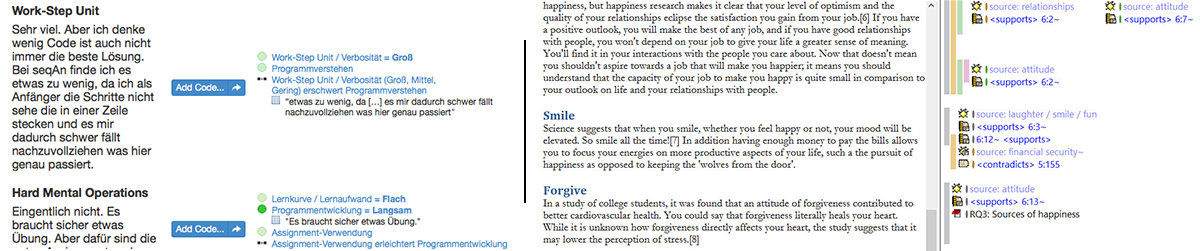
\includegraphics[width=1.0\linewidth]{Figures/apiua/codeinstances-atlas.png}
  \caption[Vergleich APIUA und ATLAS.ti: Kodeinstanz-Darstellung]{Vergleich Kodeinstanz-Darstellung; links: \gls{apiua}; rechts: \textit{ATLAS.ti}}
  \label{fig:apiua-codeinstances-atlas}
\end{figure}

\paragraph{Organisation und Sortierung von Kodes}
Im Gegensatz zur \textit{ATLAS.ti} können in \gls{apiua} Kodes gefiltert, sortiert und hierarchisch angeordnet werden (siehe \autoref{fig:apiua-codes-atlas}, links). Die Semantik der hierarchischen Modellierung wird von dem Werkzeug wie folgt behandelt: ``Wenn Kode \code{apiua://code/-9223372036854774936}\footnote{Zur Erinnerung: Es handelt sich hierbei um die Darstellung eines Kodes. Details zu dieser Stellung können im \sref{sec:notationen} auf Seite \pageref{sec:notationen} nachgelesen werden.} der Elter des Kodes \code{apiua://code/-9223372036854774934} ist, ist \code{apiua://code/-9223372036854774934} eine Ausprägung von \code{apiua://code/-9223372036854774936}, oder: \code{apiua://code/-9223372036854774936} manifestiert sich in \code{apiua://code/-9223372036854774934}.''

An dieser Stelle ist \textit{ATLAS.ti} scheinbar differenzierter. Dort können Beziehungen zwischen Elter und Kind von einer der drei Arten [\textit{Kategorie/generelles Konzept -- Kode}], [\textit{Oberbegriff -- Unterbegriff}] und [\textit{Das Ganze -- Bestandteile}] sein \citep{MuhlmeyerMentzel:2011vs}. Aber: Die Semantik dieser Beziehungen existiert nur in der Vorstellung des Forschers. Technisch handelt es sich lediglich um vordefinierte, benannte Relationstypen, die beliebig editiert werden können und von \textit{ATLAS.ti} selbst nicht weiter interpretiert werden. Im Gegensatz zu \gls{apiua} wird der Relationstyp in \textit{ATLAS.ti} nicht verwendet, um eine weitergehende Werkzeugunterstützung zu ermöglichen.

\cite{MuhlmeyerMentzel:2011vs} räumt ein, dass die Strukturierungsmöglichkeiten in \textit{ATLAS.ti} beschränkt sind. Insbesondere können Kodes nicht sortiert werden. Die Möglichkeit der hierarchischen Organisation von Kodes verändere den Arbeitsstil. Entschließt sich ein Forscher jedoch dazu, Kodes hierarchisch anzuordnen, kann er dies in \textit{ATLAS.ti} nur über die Definition von individuellen Relationen simulieren, die von der Anwendung aber nicht weiter berücksichtigt und beispielsweise nicht zur Darstellung eines Kode-Baums verwendet wird.

In \gls{apiua} kann jedes Datum, das \textit{Locatable} implementiert, auch kodiert werden. Da Kodes auch \textit{Locatable} implementieren, können Kodes andere Kodes kodieren. Um die Modellierungskomplexität nicht unnötig zu erhöhen, habe ich mich dazu entschlossen, diese Semantik mit der Eltern-Kind-Beziehung gleichzusetzen. Ist also \code{apiua://code/-9223372036854774934} ein Kind von \code{apiua://code/-9223372036854774936}, wird dies von \gls{apiua} genauso gehandhabt, als wäre \code{apiua://code/-9223372036854774934} mit \code{apiua://code/-9223372036854774936} kodiert worden.

Die eben beschriebene Beziehung gilt auch transitiv. Hat \code{apiua://code/-9223372036854774934} neben seinem Elternkode \code{apiua://code/-9223372036854774936} auch noch den Unterkode \code{apiua://code/-9223372036854774932}, so gilt: ``\code{apiua://code/-9223372036854774932} ist mit \code{apiua://code/-9223372036854774934} kodiert'' und ``\code{apiua://code/-9223372036854774932} ist mit \code{apiua://code/-9223372036854774936} kodiert''.

\paragraph{Memos} werden in APIUA umfassend unterstützt. Jedes Datum, das das \texttt{Locatable}-Interface implementiert, kann ein Memo besitzen. Das Memo des aktuell fokussierten Elements, erscheint im Memo-Editor (siehe \fref{fig:apiua-memos}). Ist das Fokus habende Element ein Kode oder eine Relation, werden optional auch sämtliche Memos der entsprechenden Kode- bzw. Relationsinstanzen gezeigt. Der Memo-Editor ist ein erweiterter, auf dem \textit{Nebula}-Browser basierender Rich-Text-Editor, der sowohl interne als auch externe Verknüpfungen zu anderen Daten erlaubt. Eine interne Verknüpfung bezieht sich auf eine \gls{uri} mit dem Schema \textit{apiua}. Klickt der Anwender auf einen solchen Link, öffnet dieser den Datenpunkt entsprechend seines Typs: Memo wird im Memo-Editor geladen, Kode wird in Kode-Ansicht hervorgehoben, Quellcode-Datei wird in der Vergleichsansicht geöffnet, etc. Verweilt der Anwender mit seiner Maus hingegen für einen kurzen Moment über einem Link (ohne ihn anzuklicken), so öffnet sich ein gelbes Informationsfenster, das wichtige --- wiederum typabhängige --- Informationen zu diesem Datenpunkt anzeigt (siehe \fref{fig:apiua-browsing}). Dieses Informationsfenster kann von anderen Plugins erweitert werden.

\begin{figure}
  \centering
    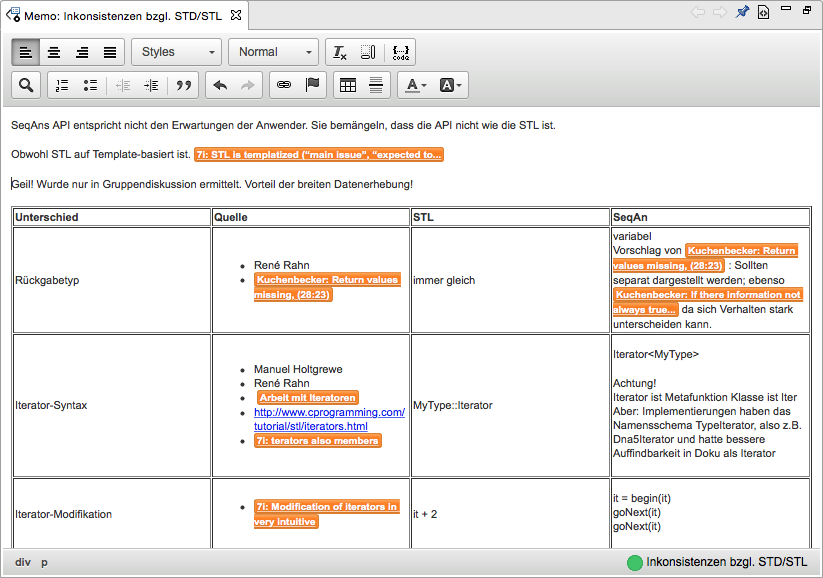
\includegraphics[width=0.8\linewidth]{Figures/apiua/memos.png}
  \caption[APIUA: Memo-Editor]{Dieser Screenshot zeigt den auf dem \textit{Nebula}-Browser basierenden Memo-Editor samt Inhalt für den Kode \url{apiua://code/-9223372036854775633}.}
  \label{fig:apiua-memos}
\end{figure}

\paragraph{Visualisierung}
Wie in \textit{ATLAS.ti} auch, können Kodes mit Farben versehen werden. Allerdings wird die Bedienung dieser Funktion von \cite{Zieris:yCXyxVc9} als umständlich und nicht für große Datenmengen geeignet, beschrieben. In \gls{apiua} kann der Anwender die Farbe eines spezifischen Kodes, eines Teilbaums oder des gesamten Kode-Bestands automatisch färben lassen. Die zweite und dritte Option skalieren auch für große Datenmengen gut. Dazu werden die Farben der Nachbarknoten berücksichtigt und ein konfliktfreier Farbraum bestimmt. Dieser wird dann rekursiv auf die Kindkodes gleich verteilt. Dadurch erhalten Kodes, die sich nah sind (gleicher Teilbaum, wenig Abstand zum Nachbarkode) eine ähnlichere Farbe als solche, die weiter voneinander entfernt sind. \fref{fig:apiua-colors} zeigt ein Beispiel. Diese Funktion hat sich als sehr nützlich für das axiale Kodieren erwiesen, da ich so ein besseren Überblick über verwandte Konzepte hatte.

\begin{figure}
  \centering
    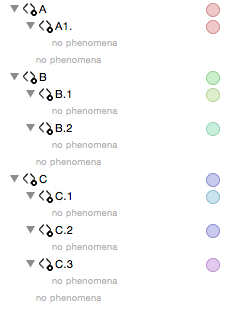
\includegraphics[width=0.4\linewidth]{Figures/apiua/colors.png}
  \caption[APIUA: Gruppendiskussion]{Dieser Screenshot von \gls{apiua} zeigt einen Kode-Teilbaum, der automatisch eingefärbt wurde. Auf den Elternkodes \code{apiua://code/-9223372036854774928}, \code{apiua://code/-9223372036854774927} und \code{apiua://code/-9223372036854774926} wird das gesamte Farbspektrum von Rot über Grün bis hin zu Violett verwendet. Die Kindkodes erhalten Farben, die links und rechts von der Elternfarbe liegen ohne den Bereich eines Nachbarteilbaums zu verletzen. Beispiel: Die Farbe von \code{apiua://code/-9223372036854774924} liegt links von \code{apiua://code/-9223372036854774927}; die von \code{apiua://code/-9223372036854774923} rechts davon.}
  \label{fig:apiua-colors}
\end{figure}

\paragraph{Eigenschaften}
In \gls{apiua} kann jeder Kode eine Dimension haben. Die zugrunde liegende Skala kann aktuell nominal oder ordinal sein\footnote{Die zur Verfügung stehenden Skalentypen können durch Plugins erweitert werden.}. Dimensionalisierte Kodes können als Eigenschaften anderer Kodes dienen. Ist ein Phänomen mit einem Kode kodiert worden, können dem Phänomen, in Bezug auf die Dimension und Eigenschaften des Kodes, Werte zugewiesen werden (siehe \autoref{fig:apiua-properties}).
\\Beispiel: Der Kode \code{Auto} verfügt über eine Eigenschaft \code{Farbe} mit der nominalen Skala \textit{(Rot, Gelb, Grün, Blau)}. Wird nun ein Phänomen \code{X} mit \code{Auto} kodiert, kann \code{X} nun ein Wert für die \textit{Farbe} zugewiesen werden, denn \code{X} ist fortan eine Instanz/Ausprägung/Phänomen für \code{Auto}.

Diese Art der Implementierung der \gls{gtm} erlaubt sogar \textit{Subdimensionalisierung} \citep{strauss1987qualitative}, also die Modellierung von Eigenschaften, die selbst wiederum Eigenschaften besitzen. Am Beispiel der Autofarbe könnte eine Untereigenschaft von Farbe die Eigenschaft \textit{Lackierung} \textit{(matt, glänzend)} sein.

\paragraph{Schwierigkeiten der Modellierung} von Analyseergebnissen ergeben sich bei der Verwendung hierarchischer Kodes und Eigenschaften:

\begin{description}
  \item[Spezifität] \hfill \\
  Während der Analyse meiner subjektiven Daten musste ich feststellen, dass die getroffenen Aussagen inhaltlich derart in die Breite gingen, dass ich für jeden generierten Kode kaum eine nennenswerte Zahl Verankerungen hatte. In solch einem Fall könnte man \textit{theoretischen Samplings} betreiben, indem man weitere Daten erhebt, um diese Kodes besser verstehen zu können. Allerdings kann eine solche Datenerhebung sehr teuer sein und ein Mittelweg muss gefunden werden.
  
  Konkretes Beispiel: In meinen Daten schildert\citepurl{apiua://survey/cd/2013-09-19T11:51:16.616+02:00/hardMentalOperations} ein Proband seine Frustration von dem Templatemetaprogrammiungs-Aspekt \textit{Metafunktion}, was ich mit dem Kode \code{apiua://code/-9223372036854775514} kodierte. Dieser Kode ist selbst ein Unterkode von \code{apiua://code/-9223372036854775515}. An anderer Stelle gibt es eine weniger spezifische Aussage\citepurl{apiua://survey/cd/2013-09-19T11:51:16.616+02:00/workStepUnit}, in der nur noch allgemein von \textit{Templatemetaprogramming} die Rede ist.
  
  \medskip
  
  \begin{center}
    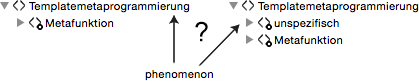
\includegraphics[width=0.7\linewidth]{Figures/apiua/problem-specificity.png}
  \end{center}
  
  Hier stellt sich nun die Frage, ob die allgemeinere Aussage mit \code{apiua://code/-9223372036854775515} kodiert werden sollte. Oder man führt einen ``unspezifischen'' Unterkode von \code{apiua://code/-9223372036854775515} ein und verwendet diesen dann als ``Sammelbecken'' für Phänomene mit geringerem Aussagegehalt.
  
  
  
  \item[Vererbung] \hfill \\
  Welche Auswirkungen haben Eigenschaften eines Kodes auf seine Eltern- bzw. Kindkodes? Denkt man an Objektorientierung, hieße die Antwort, dass Eigenschaften nach unten vererbt werden. Aber gilt das auch für Kodeinstanzen? Würden wir uns beim obigen Beispiel für die erste Variante entscheiden, würde das Phänomen nicht nur eine Instanz von \code{apiua://code/-9223372036854775515} darstellen, sondern auch von allen Unterkodes von \code{apiua://code/-9223372036854775515}, u.a. auch \code{apiua://code/-9223372036854775514}. Ob sich ein Phänomen auf alle Unterformen bezieht oder schlichtweg nur eine geringe Aussagekraft hat, kann man nicht immer zuverlässig sagen. Oder gilt die Vererbung von Kodeinstanzen gar nach oben? Immerhin sollten sich Aussagen über \code{apiua://code/-9223372036854775515} treffen lassen, wenn man konkretere Phänomene zu \code{apiua://code/-9223372036854775514} gesehen hat. 
  
  Meinen Lösungsvorschlag für diese Problemfragen gebe ich weiter unten. 
\end{description}

\begin{figure}
  \centering
    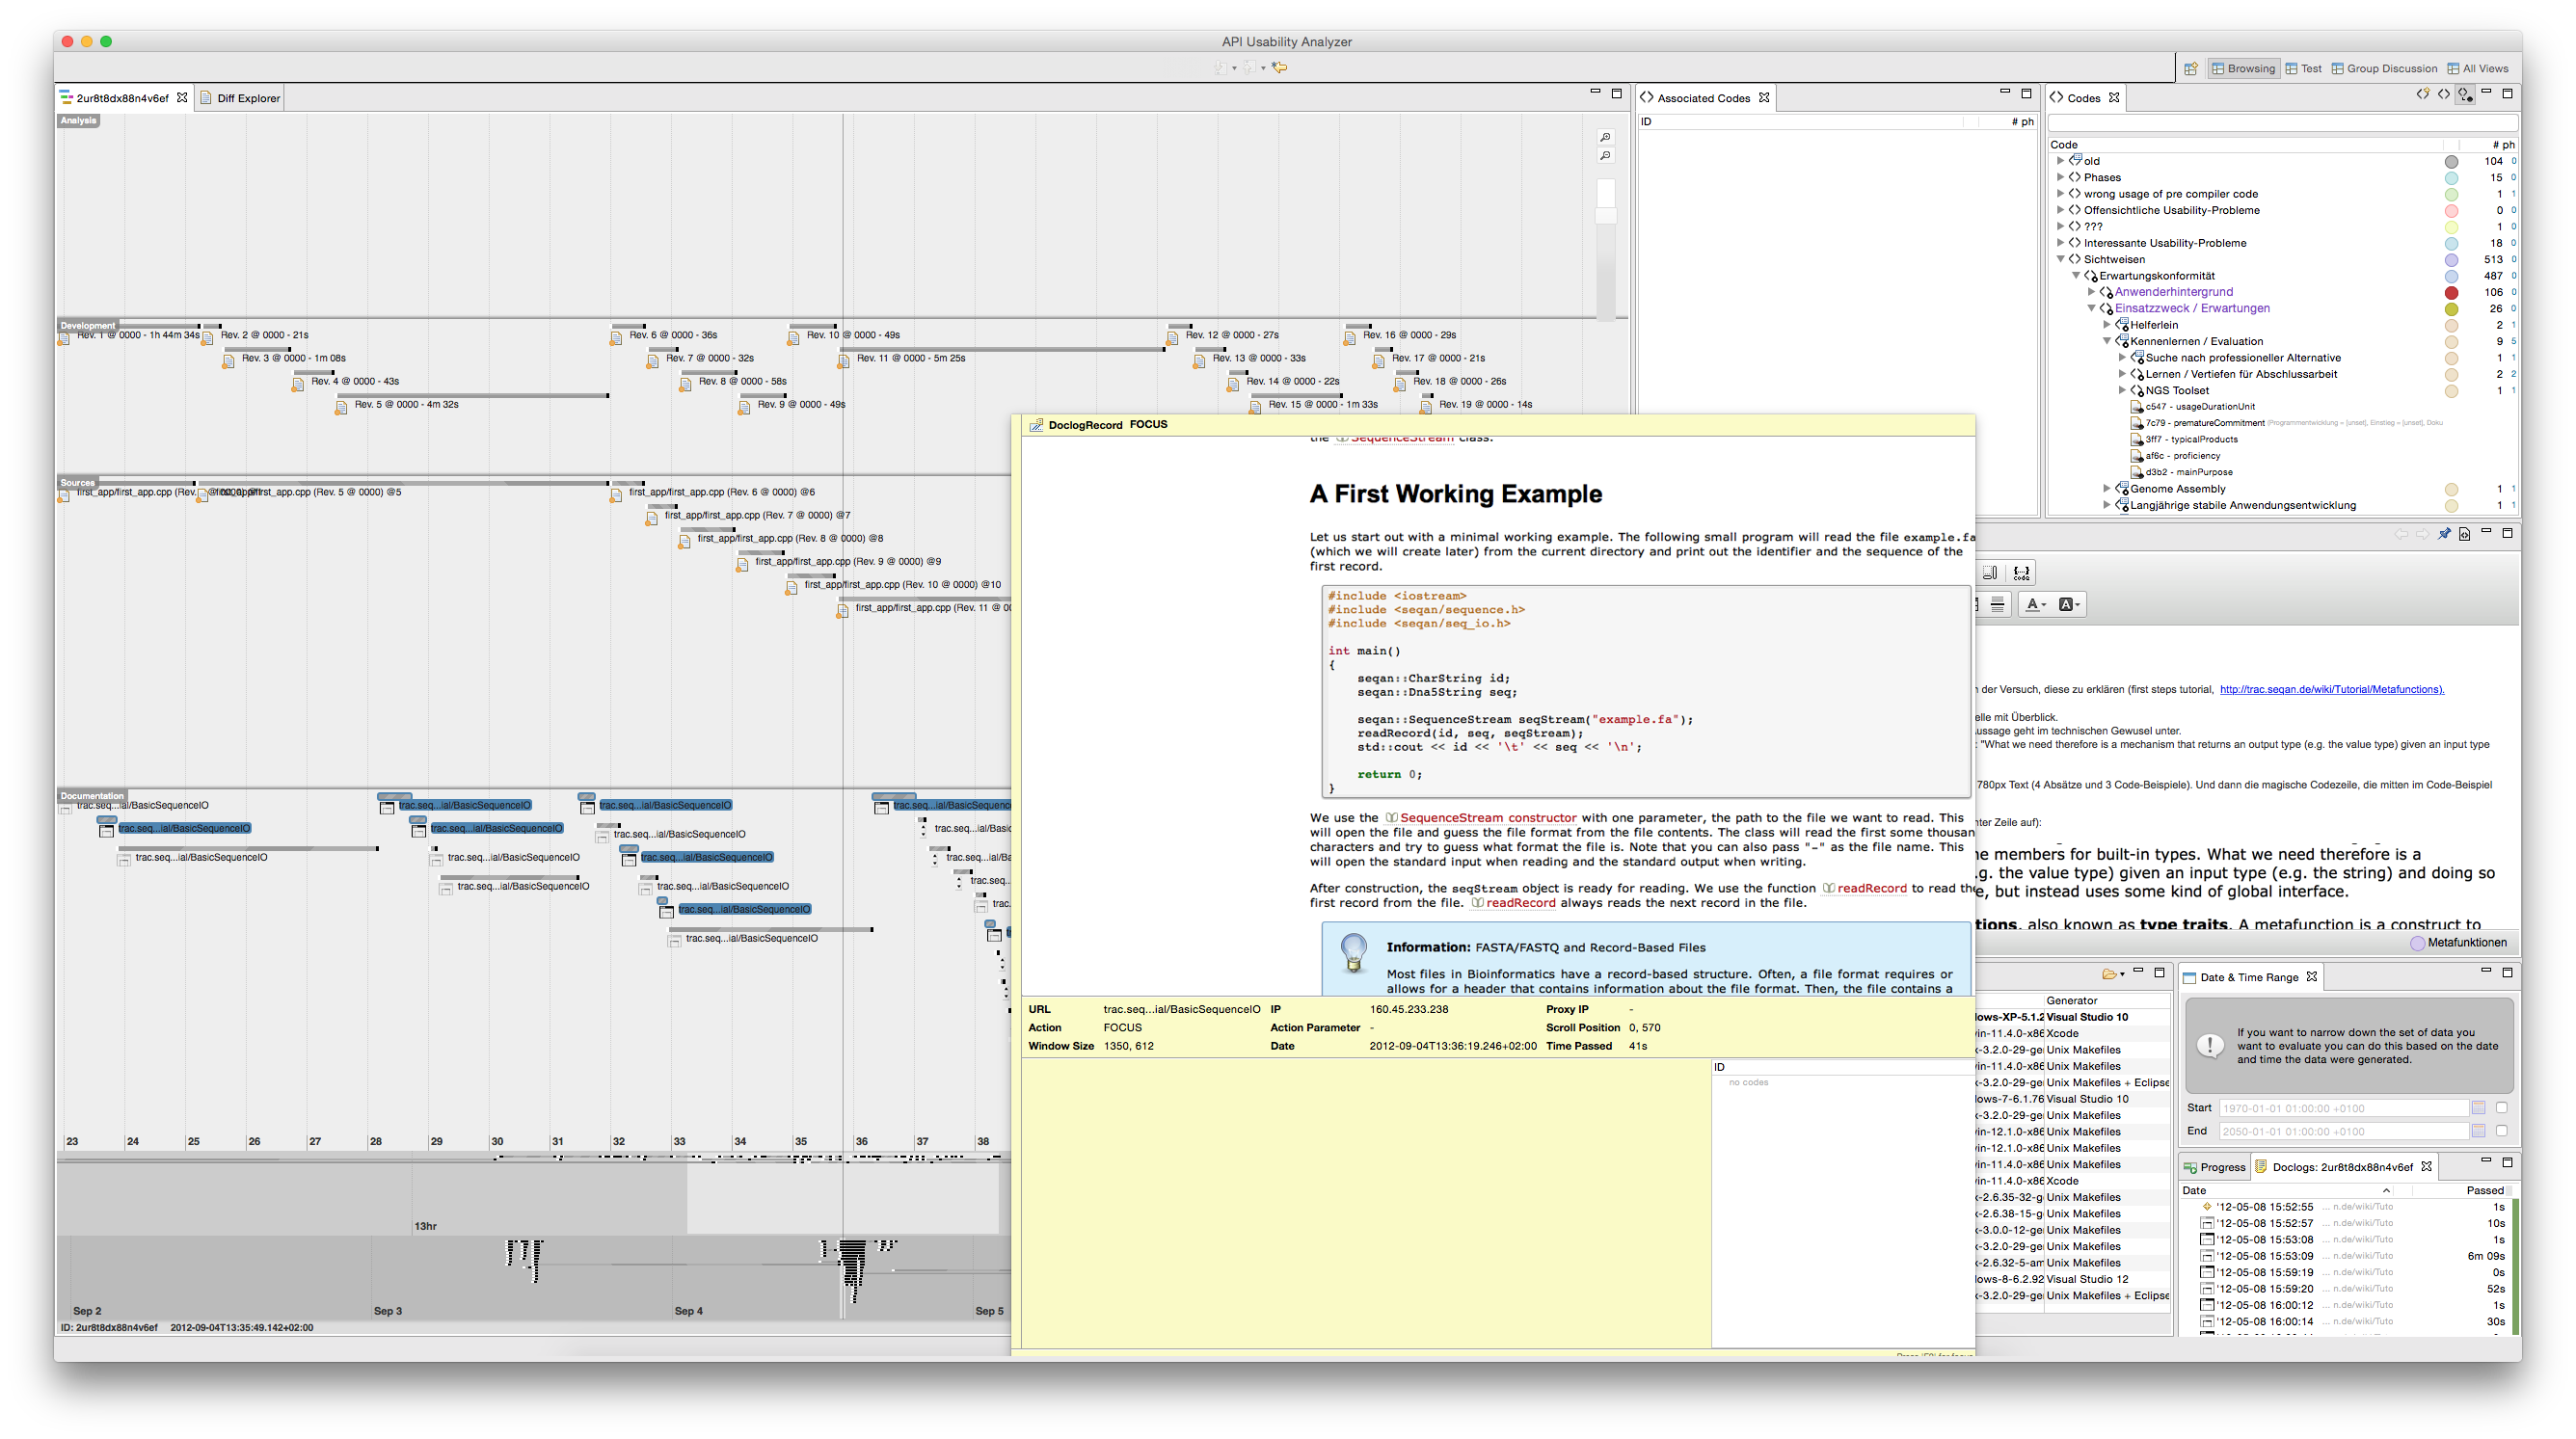
\includegraphics[width=1.0\linewidth]{Figures/apiua/browsing.png}
  \caption[APIUA: Exploration]{Dieser Screenshot von \gls{apiua} zeigt eine typische Analysesitzung, bei der sich der Forscher einen Überblick über die Daten verschafft. Dazu nutzt er die Zeitleistenansicht.}
  \label{fig:apiua-browsing}
\end{figure}

\begin{figure}
  \centering
    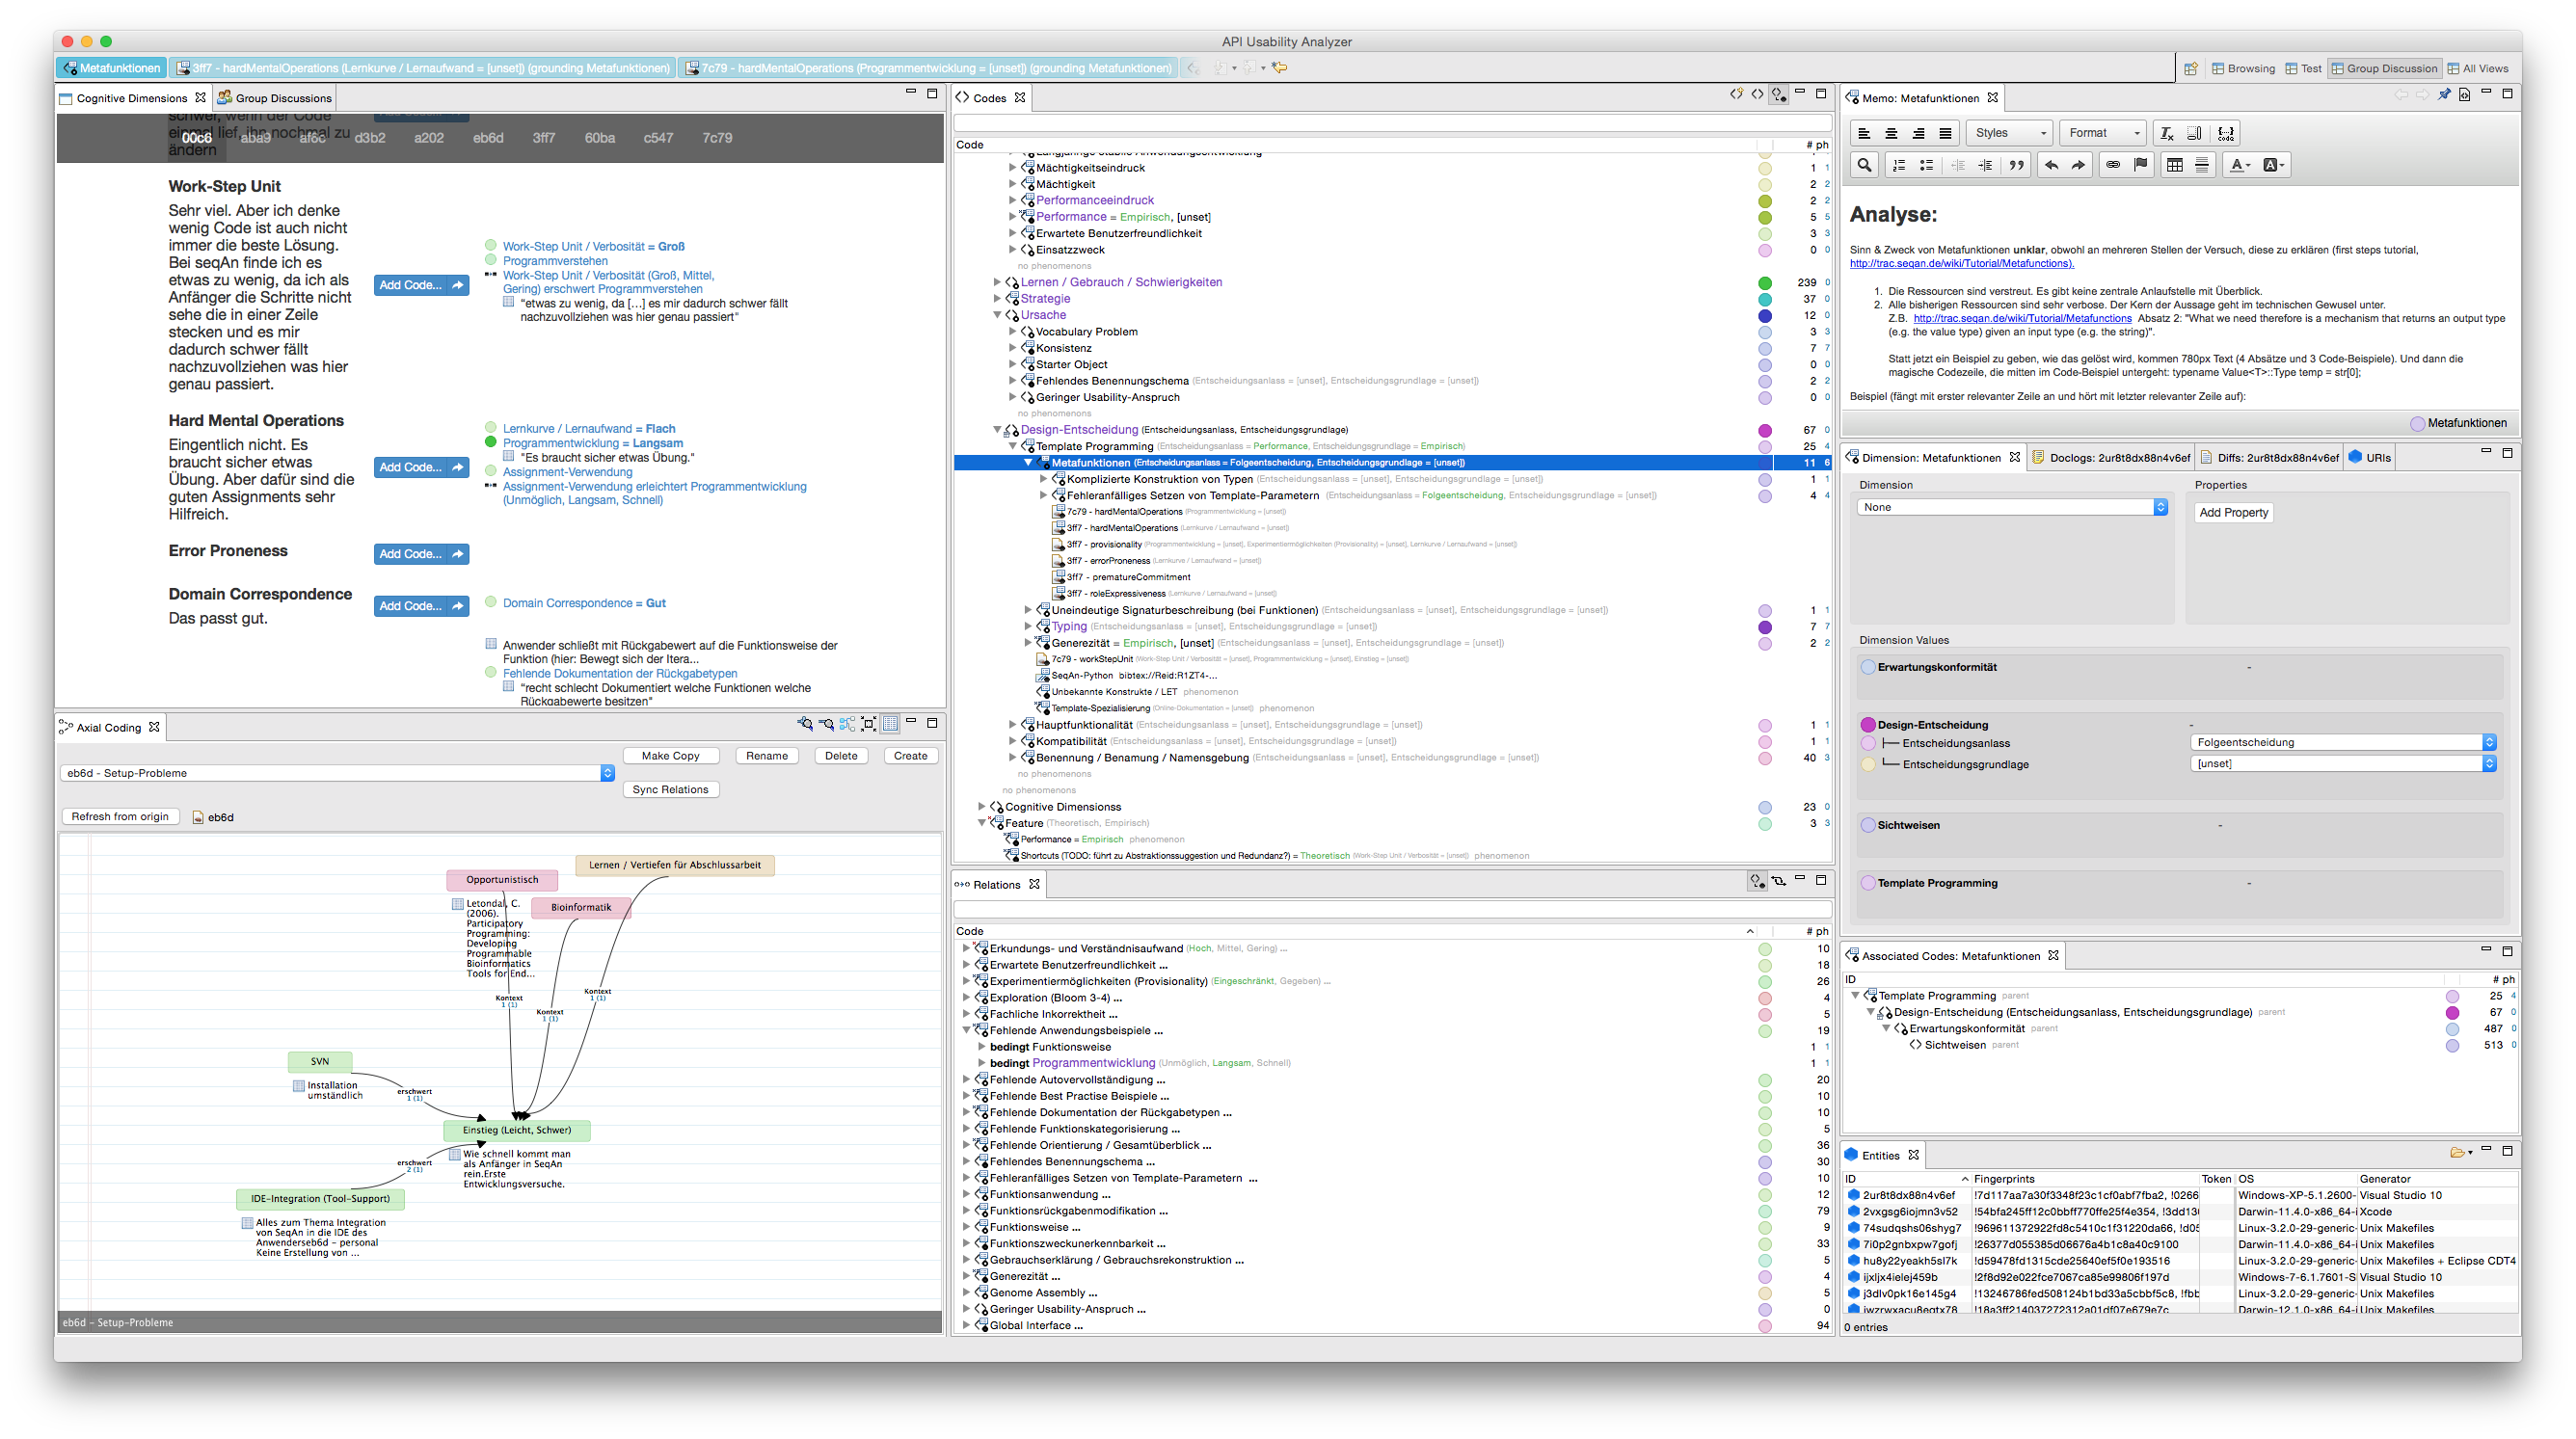
\includegraphics[width=1.0\linewidth]{Figures/apiua/opencoding-cd.png}
  \caption[APIUA: Cognitive Dimensions]{Dieser Screenshot von \gls{apiua} zeigt eine typische Sitzung mit Fokus auf offenes Kodieren. In diesem Fall werden die Cognitive-Dimensions-Fragebögen (oben links) analysiert.}
  \label{fig:apiua-opencoding-cd}
\end{figure}

\begin{figure}
  \centering
    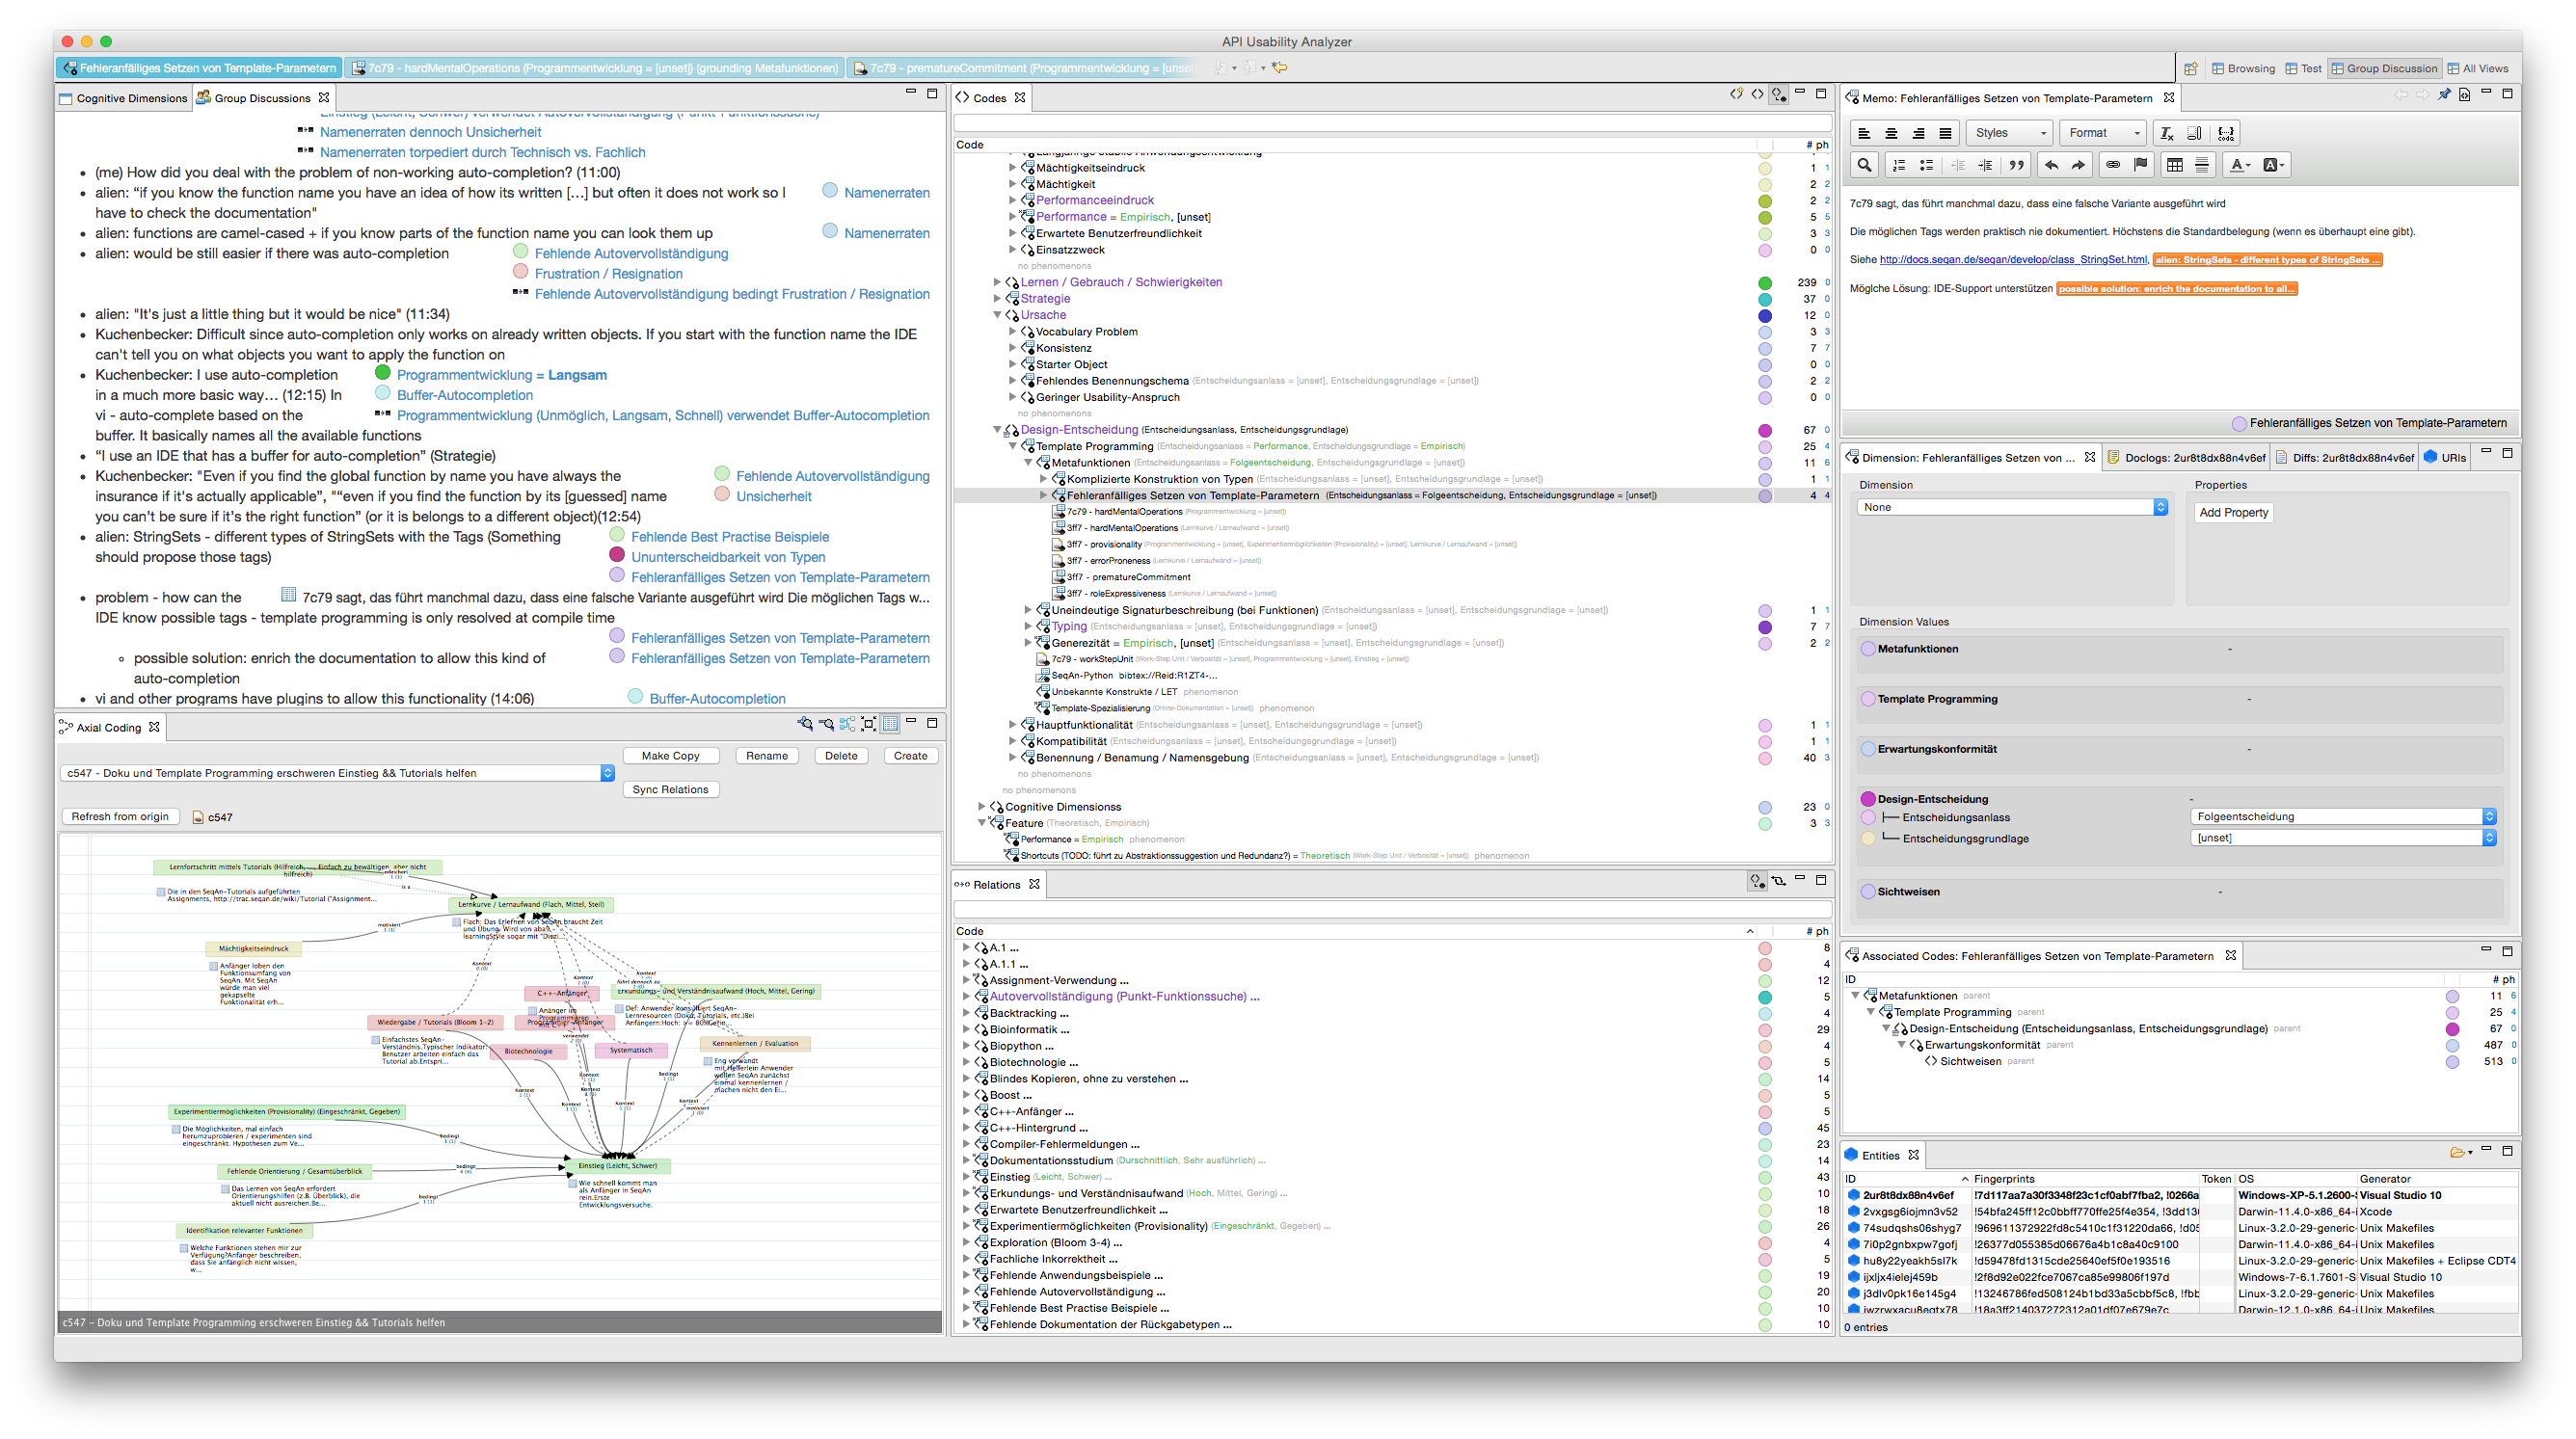
\includegraphics[width=1.0\linewidth]{Figures/apiua/opencoding-gd.png}
  \caption[APIUA: Gruppendiskussion]{Dieser Screenshot von \gls{apiua} zeigt eine typische Sitzung mit Fokus auf offenes Kodieren. In diesem Fall wird eine Gruppendiskussion (oben links) betrachtet.}
  \label{fig:apiua-opencoding-gd}
\end{figure}

Nach der \gls{gtm} von \cite{strauss1990basics,corbin2014basics} ``darf'' auch das Vorwissen des Forschers in den Forschungsprozess eingebracht werden. Die \textit{\acrshort{uri}}-Komponente von \acrshort{apiua} erlaubt das Erfassen \acrshort{uri}-referenzierbarer Quellen. Dies ermöglicht es dem Forscher Konzepte in beliebigen Dokumenten zu verankern, auf das sein Vorwissen fußt. In meiner Forschung habe ich Verankerungen ganz konkret auf Basis von Literatur mit Hilfe von \url{bibtex:}-\acrshort{uri}s und verschiedenartigste Dokumente mit Hilfe von \url{file:}-\acrshort{uri}s vorgenommen. Dieses Vorgehen ist aus meiner Sicht unerlässlich, um die Gütekriterien \textit{Argumentative Interpretationsabsicherung} und \textit{Nähe zum Gegenstand} zu erfüllen. Keines der mir bekannten CAQDAS-Anwendungen erfüllt diese Anforderungen, ohne dass die referenzierten Dokumente auch direkt in das Datenanalysewerkzeug importiert und damit auch von dem Werkzeug unterstützt werden müssten.




\subsubsection{Axiales Kodieren}
\label{sec:apiua-axial-coding}

Die Möglichkeit axial kodieren zu können, ist ein integraler Bestandteil von \gls{apiua}. Eine Relation in \gls{apiua} ist wie ein benannter gerichteter Graph zwischen zwei Kodes und wird in dieser Arbeit wie folgt notiert: \rel[Bezeichner]{\code{Kode 1}}{\code{Kode 2}}. \autoref{fig:apiua-axialcoding} zeigt die entsprechende Ansicht in APIUA. So wie Kodes mit Hilfe von Kodeinstanzen verankert werden, können auch Relationen mittels Relationsinstanzen verankert werden.

\textit{ATLAS.ti} verwendet zwar für Kodes ein vergleichbares Datenmodell \citep{MuhlmeyerMentzel:2011vs}, kann aber Relationen selbst nicht verankern \citep{Zieris:yCXyxVc9}. Möchte der Forscher also nachschauen, auf welchen Datenpunkten eine Relation überhaupt fußt, besteht für ihn nur die Möglichkeit, alle Stellen zu ermitteln, die als Verankerungen für die beiden, durch die Relation in Beziehung gesetzten Kodes dienen und in Gedanken neu zu kodieren.

Kurzum: Wenn der Forscher das Verankerungsproblem nicht auf andere Weise gelöst hat, können Verankerungen von Relationen durch Dritte nur eingeschränkt nachvollzogen werden, was aus meiner Sicht die Verifizierbarkeit von mit \textit{ATLAS.ti} erstellten Relationen potentiell einschränkt.

Eine weitere Einschränkung in \textit{ATLAS.ti} besteht darin, dass es zwischen zwei Kodes nur eine Relation geben kann. \gls{apiua} unterstützt beliebig viele --- wenn der Forscher es für notwendig hält auch gleich benannte --- Relationen.

\begin{figure}
  \centering
    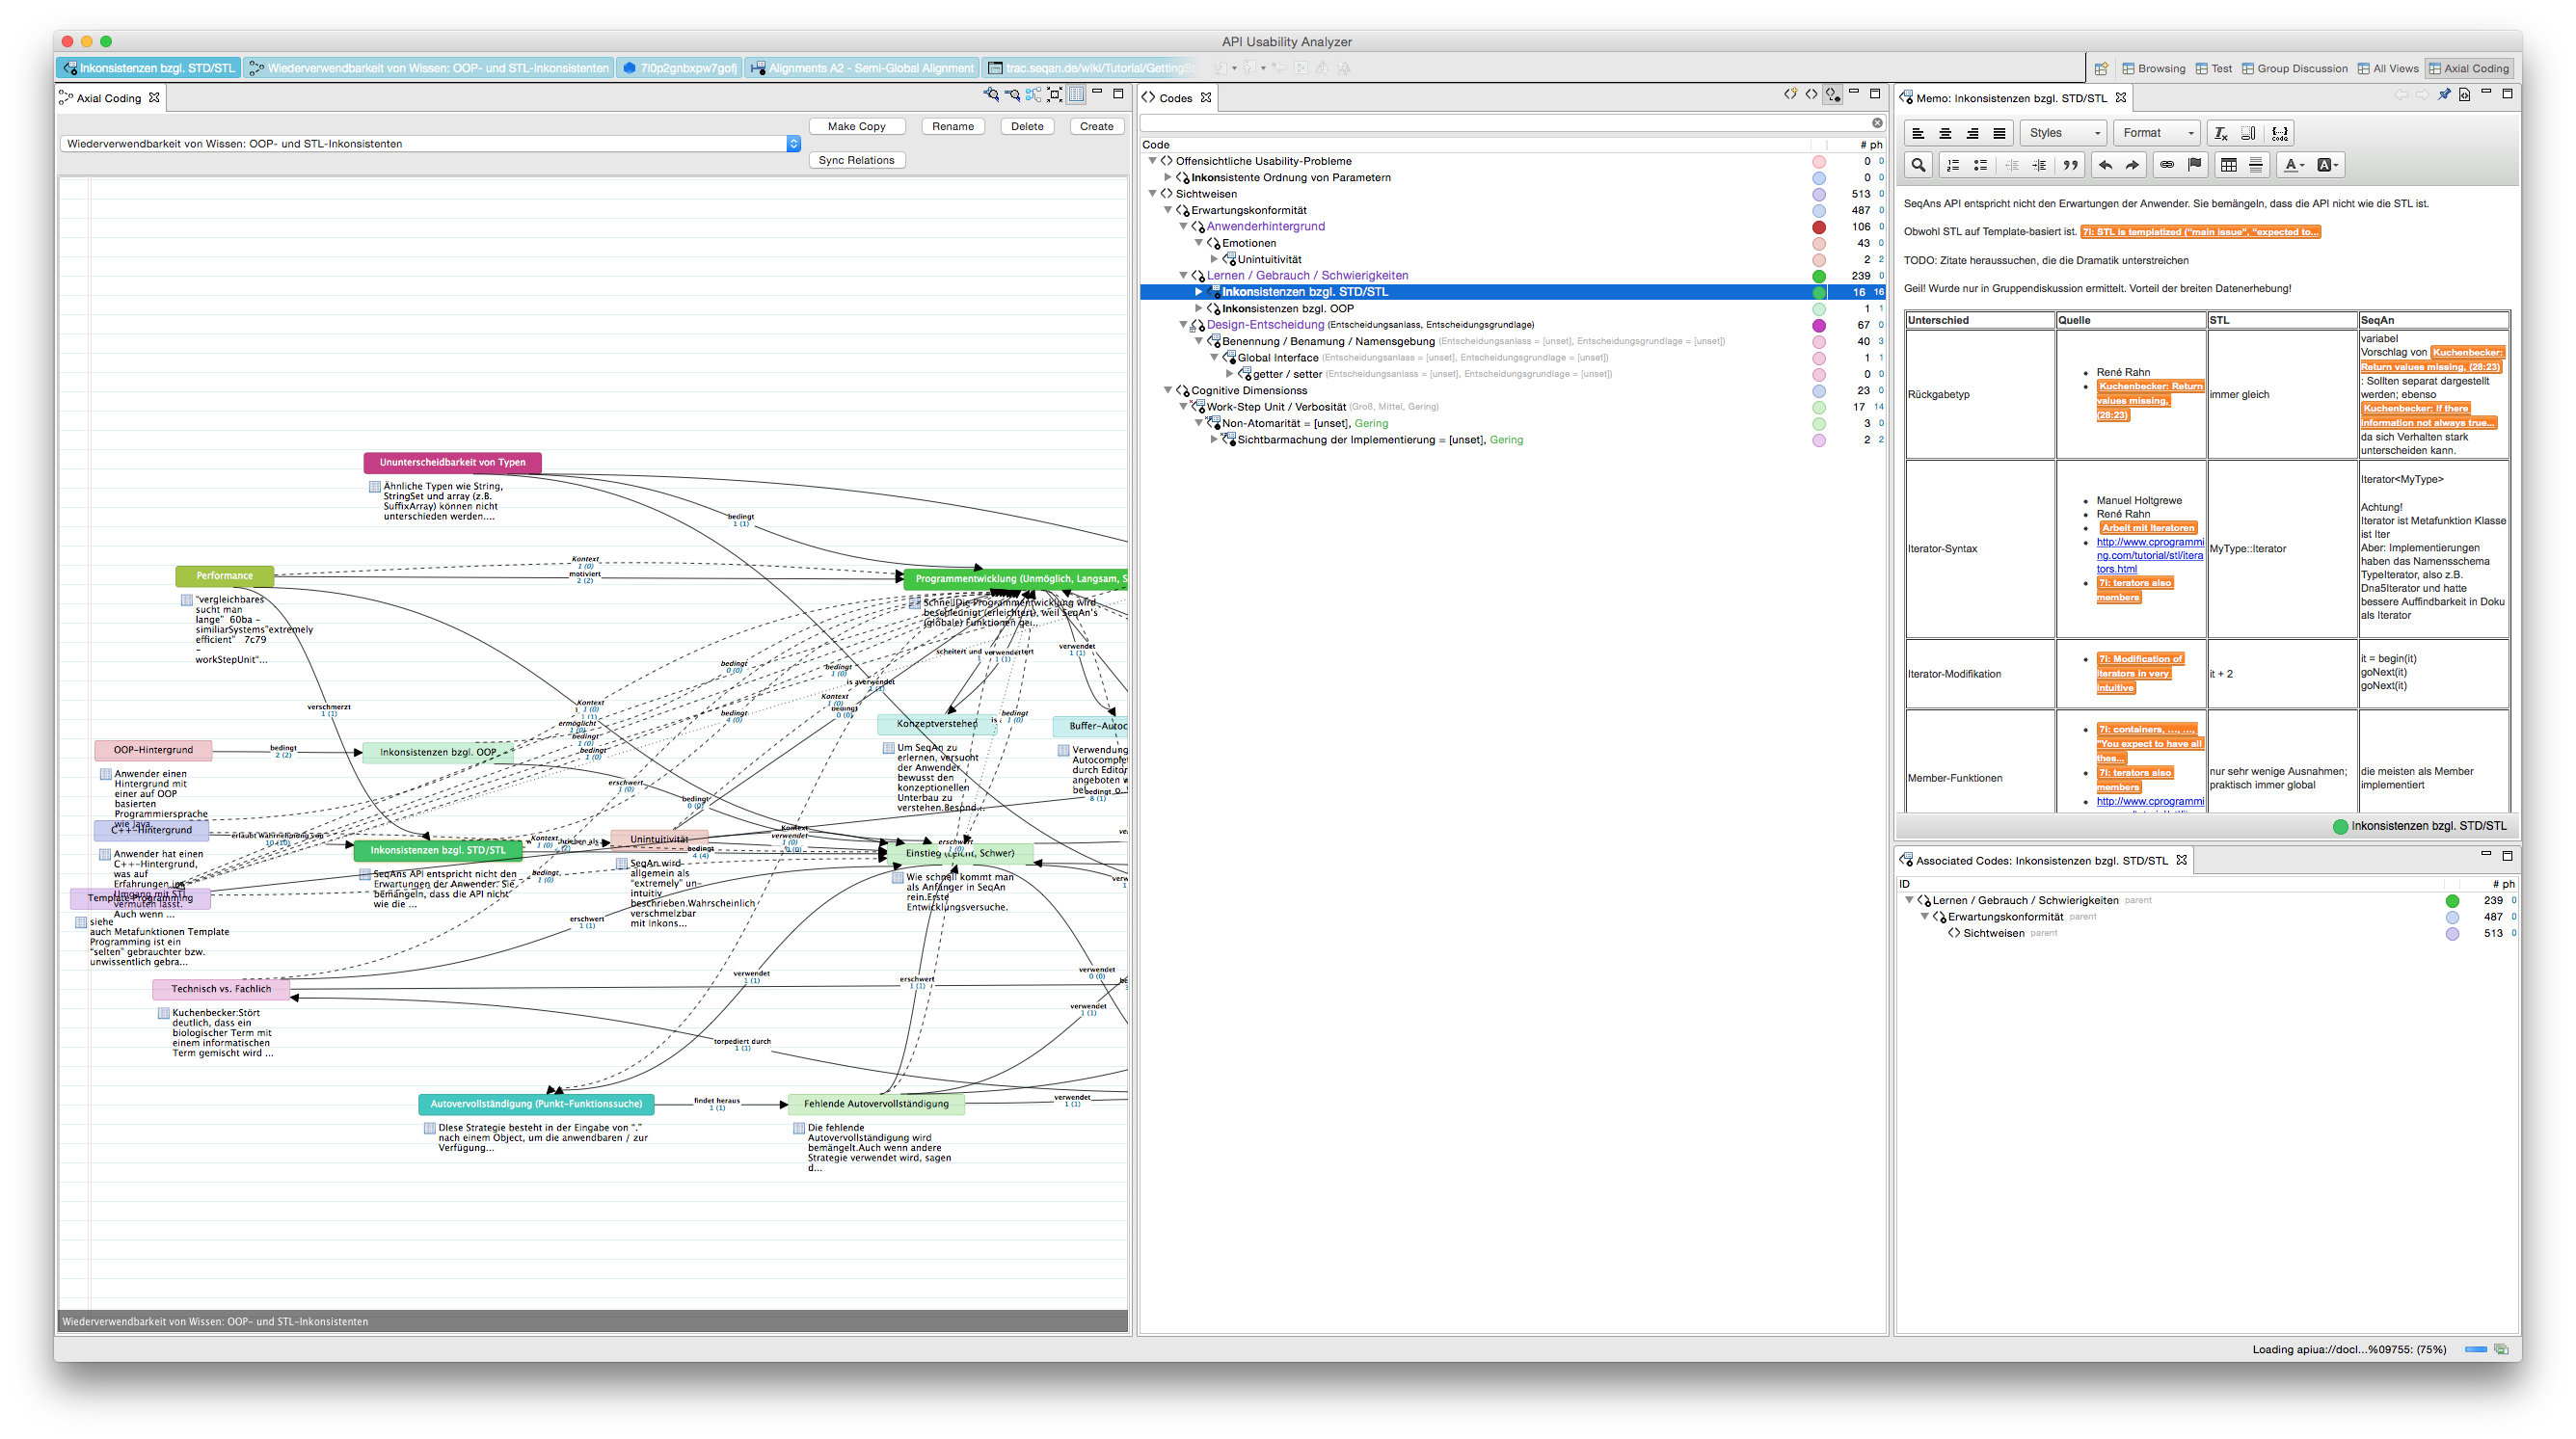
\includegraphics[width=1.0\linewidth]{Figures/apiua/axialcoding.png}
  \caption[APIUA: Axiales Kodieren ]{Dieser Screenshot von \gls{apiua} zeigt eine typische Sitzung mit Fokus auf axiales Kodieren. In diesem Fall wird das \glslink{acm}{axiale Kodiermodell} ``OOP- u. STL-Inkonsistenzen'' --- links dargestellt --- bearbeitet.}
  \label{fig:apiua-axialcoding}
\end{figure}

Der Forscher hat zwei verschiedene Möglichkeiten \glspl{ac} bzw. \glspl{acm}\footnote{Zur Erinnerung: Eine \gls{ac} stellt Relationen auf Kodeinstanz-Ebene dar, wohingegen ein \gls{acm} Relationen auf Kode-Ebene beschreibt.} zu erstellen. Entweder beginnt er ``from scratch'', entwickelt also eines von Grund auf oder er erstellt eines auf der Grundlage eines existierenden Kodes, einer existierenden Relation oder einer jeweiligen Instanz. In beiden Fällen hält der Editor den Graphen bei Änderungen (Umbenennungen, Farbänderungen, Hierarchieänderungen, etc.) aktuell. Im zweiten Fall wird darüber hinaus der Graph selbst dynamisch erzeugt, initial formatiert und ebenfalls aktuell gehalten. Der so erstellte Graph enthält alle Kodes bzw. Kodeinstanzen, mit denen der ursprünglich ausgewählte Kode bzw. die Kodeinstanz über Relationen verbunden ist. Gibt es also \rel{\code{apiua://code/-9223372036854774936}}{\code{apiua://code/-9223372036854774935}} und basiert der Graph auf \code{apiua://code/-9223372036854774936}, enthält der Graph neben \code{apiua://code/-9223372036854774936} auch \code{apiua://code/-9223372036854774935} und \rel{\code{apiua://code/-9223372036854774936}}{\code{apiua://code/-9223372036854774935}}. Für Elemente, die für den Aussagekern des \glslink{acm}{axialen Kodiermodells} unwichtig sind, besteht die Möglichkeit, sie auszublenden.

Zurück zum obigen Beispiel: Ein Proband machte eine Aussage\citepurl{apiua://survey/cd/2013-09-19T11:51:16.616+02:00/hardMentalOperations} zu Metafunktionen. Genauer: Die Notwendigkeit, sich mit Metafunktionen auseinanderzusetzen, wird als frustrierend beschrieben. Daraus ergibt sich \rel[bedingt]{\code{apiua://code/-9223372036854775514}}{\code[apiua://code/-9223372036854775314]{Frustration/Resignation}}. Eine andere Aussage\citepurl{apiua://survey/cd/2013-09-19T11:51:16.616+02:00/workStepUnit} ist ähnlich, aber weniger spezifisch: \rel[bedingt]{\code{apiua://code/-9223372036854775515}}{\code[apiua://code/-9223372036854775314]{Frustration/Resignation}}.

Durch die Unterstützung von Unter- und Überkodes könnte man nun definieren, dass \rel[bedingt]{\code{apiua://code/-9223372036854775514}}{\code[apiua://code/-9223372036854775314]{Frustration/Resignation}} eine Unterrelation von \rel[bedingt]{\code{apiua://code/-9223372036854775515}}{\code[apiua://code/-9223372036854775314]{Frustration/Resignation}} ist. Oder allgemeiner: Ist \code{apiua://code/-9223372036854774934} Unterkode von \code{apiua://code/-9223372036854774936} und \code{apiua://code/-9223372036854774933} Unterkode von \code{apiua://code/-9223372036854774935}, wären \rel[x]{\code{apiua://code/-9223372036854774934}}{\code{apiua://code/-9223372036854774935}}, \rel[x]{\code{apiua://code/-9223372036854774936}}{\code{apiua://code/-9223372036854774933}} und \rel[x]{\code{apiua://code/-9223372036854774934}}{\code{apiua://code/-9223372036854774933}} Unterrelationen von \rel[x]{\code{apiua://code/-9223372036854774936}}{\code{apiua://code/-9223372036854774935}} (\textit{x} ist ein beliebiger gemeinsamer Bezeichner; siehe \autoref{fig:SubRelations}).

\begin{figure}
  \centering
    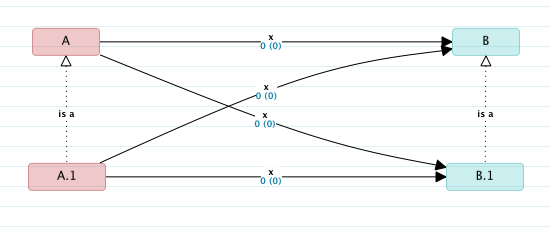
\includegraphics[width=1.0\linewidth]{Figures/sub_relations.png}
  \caption[APIUA: Modellierung --- Unterrelationen]{Die Relationen \rel[x]{\code{apiua://code/-9223372036854774934}}{\code{apiua://code/-9223372036854774935}}, \rel[x]{\code{apiua://code/-9223372036854774936}}{\code{apiua://code/-9223372036854774933}} und \rel[x]{\code{apiua://code/-9223372036854774934}}{\code{apiua://code/-9223372036854774933}} sind Unterrelationen von \rel[x]{\code{apiua://code/-9223372036854774936}}{\code{apiua://code/-9223372036854774935}}.}
  \label{fig:SubRelations}
\end{figure}

Auch diese Konstruktion ist wie bei den Kodes transitiv. Hätte \code{apiua://code/-9223372036854774934} den Unterkode \code{apiua://code/-9223372036854774932} und \code{apiua://code/-9223372036854774933} den Unterkode \code{apiua://code/-9223372036854774931} und gäbe es die Relationen \rel[x]{\code{apiua://code/-9223372036854774936}}{\code{apiua://code/-9223372036854774935}}, \rel[x]{\code{apiua://code/-9223372036854774934}}{\code{apiua://code/-9223372036854774933}} und \rel[x]{\code{apiua://code/-9223372036854774932}}{\code{apiua://code/-9223372036854774931}} so wäre nicht nur \rel[x]{\code{apiua://code/-9223372036854774934}}{\code{apiua://code/-9223372036854774933}} Unterrelation von \rel[x]{\code{apiua://code/-9223372036854774936}}{\code{apiua://code/-9223372036854774935}} sondern auch \rel[x]{\code{apiua://code/-9223372036854774934}}{\code{apiua://code/-9223372036854774933}} Unterrelation von \rel[x]{\code{apiua://code/-9223372036854774936}}{\code{apiua://code/-9223372036854774935}}.

So wie Kodes Kodeinstanzen haben können, können Relationen auch Relationsinstanzen besitzen. Hier stellt sich dieselbe Vererbungsfrage wie bei Kodes: Erben Unterrelationen die Instanzen ihrer Überrelation (oder anders herum)? Und wie kodiere ich unspezifische Aussagen?


\subsubsection{Selektives Kodieren}
\label{sec:apiua-selective-coding}

In \textit{ATLAS.ti} gibt es keine explizite Unterstützung für selektives Kodieren. Von dem Forscher wird erwartet, dass er dazu die vorhandene Funktionalität der Software nutzt. Dazu zählen insbesondere die für das axiale Kodieren bereitgestellten Möglichkeiten.

Ähnlich verfährt auch \gls{apiua} --- mit zwei Ausnahmen:
\begin{enumerate}
	\item \gls{apiua} implementiert in Ansätzen, die Möglichkeit, Interferenzregeln auf die erarbeitete theoretische Modellierung anzuwenden, was das selektive Kodieren unterstützen kann. Dabei handelt es sich um eine Funktion, die keine der mir bekannten Konkurrenzprodukte unterstützt.
	\item Darüber hinaus gibt es die Möglichkeit, einem Kode eine Hervorhebungsgruppe zuzuordnen. Standardmäßig werden Kodes nicht hervorgehoben. Der Anwender hat die Möglichkeit die Hervorhebung abzusenken --- die schwarze Kodebeschriftung wird dann plattformweit \textcolor{gray}{grau} und die Kodefarbe blass dargestellt --- oder sie anzuheben --- dann wird die Kodebeschriftung \textbf{\textcolor{violet}{fett und violett}} und die Kodefarbe kräftiger dargestellt (siehe \fref{fig:apiua-opencoding-cd}). Auf diese Weise kann der Forscher in jeder Phase seiner Forschung Kandidaten für selektives Kodieren festhalten.
\end{enumerate}




\subsubsection{Erkenntnisperspektive}
\label{sec:Erkenntnisperspektive}

In den vorangegangenen Abschnitten habe ich Fragen aufgeworfen, die die konkrete Modellierung einer \acrfull{gt} innerhalb eines Datenanalysewerkzeugs betreffen. Sie betreffen einerseits den Umgang mit Aussagen geringerer Spezifität und andererseits die Vererbung von Erkenntnissen. Diese Fragen stellten sich mir bei dem Versuch, automatisch generierte \glspl{gtm} zu verallgemeinern und ihre wesentliche Aussage herauszuarbeiten (siehe \sref{sec:Datenanalyse-STL-Inkonsistenzen-vereinfachen}).

Als \textit{Erkenntnisperspektive} bezeichne ich, ob der Forscher entweder gerade eine synthetische (abduktiv oder induktiv -- also ``Erkenntnis erweiternd'') oder deduktive \citep{Rehfus:2003ti} Sichtweise einnimmt. Während der Entwicklung einer \gls{gt} nimmt der Forscher häufig die synthetische Erkenntnisperspektive ein, denn in ihr besteht ja gerade der Erkenntnisgewinn. Genauso häufig aber wechselt er in die deduktive Erkenntnisperspektive, um seine Hypothesen zu überprüfen \citep{kelle1994empirisch}. Dieser Wechsel zwischen Induktion und Deduktion findet während des gesamten Forschungszeitraums statt \citep[siehe \sref{sec:gtm} und][]{strauss1987qualitative}.

Mit einer deduktiven Erkenntnisperspektive sollte es sich wie bei der Objektorientierung verhalten: Die Vererbung findet von oben nach unten statt. Aussagen, die ich für Überkodes bzw. Überrelationen treffen kann, müssen --- wenn die \gls{gt} funktioniert --- auch für deren Unterkodes bzw. Unterrelationen gelten\footnote{Ganz so streng ist die Prämisse nicht, und soll auch so nicht verstanden werden. Die theoretische Konstruktion verfügt lediglich über eine ``Aura der Objektivität'' (``aura of objectivity'') und darf nicht für ein ``erzwungenes Rahmenwerk'' (``forced framework'') gehalten werden. \citep{charmaz2006constructing}\\ Eine \gls{gt}, die tatsächlich jede Beobachtung vollumfänglich erklären kann, würde Gefahr laufen, sehr deskriptiv zu werden und sich nicht mehr dazu eignen, verallgemeinerbare Aussagen zu treffen.}. 

Mit einer synthetischen Erkenntnisperspektive hingegen kann man eine hypothetische Vererbung nach oben in Erwägung ziehen. So könnten Aussagen, die für Unterkodes gelten möglicherweise auch für den Überkode gelten.

\gls{apiua} soll den bereits von \cite{Glaser:1967ts} als erforderlich beschrieben Wechsel zwischen induktivem und deduktivem Denken --- insbesondere beim axialen Kodieren \citep{strauss1990basics} --- Werkzeug-seitig unterstützen. Darum ist \gls{apiua} dem Forscher beim Einnehmen der synthetischen Erkenntnisperspektive bereits jetzt schon behilflich, indem es zum Beispiel zwischen expliziten und impliziten Relationen unterscheidet. Eine explizite Relation \relation{R} ist eine, die vom Forscher modelliert wurde. Eine implizite Relation hingegen basiert auf einer anderen explizit definierten Relation \relation{R\_}, die selbst Unterrelation von \relation{R} ist und damit \relation{R} impliziert (siehe \autoref{fig:ImplicitRelations}). Existiert \relation{R} allerdings (noch) nicht, fungiert \relation{R\_} als hypothetische Relation für ein mögliches \relation{R}. %Oder genauer: \relation{R\_} stellt für alle erdenklichen Überrelationen eine hypothetische Relation dar (siehe Abbildungen \ref{fig:ProposedRelations1}, \ref{fig:ProposedRelations2} und \ref{fig:ProposedRelations3}).

\begin{figure}
  \centering
    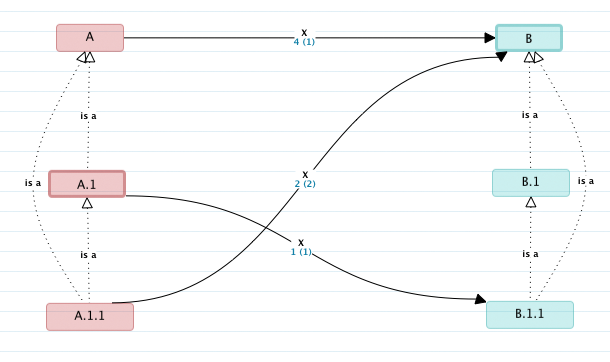
\includegraphics[width=1.0\linewidth]{Figures/implicit_relations.png}
  \caption[APIUA: Modellierung --- Implizite Relationen]{Die Relationen \rel[x]{\code{apiua://code/-9223372036854774934}}{\code{apiua://code/-9223372036854774931}}, sowie \rel[x]{\code{apiua://code/-9223372036854774932}}{\code{apiua://code/-9223372036854774935}} sind implizit für \rel[x]{\code{apiua://code/-9223372036854774936}}{\code{apiua://code/-9223372036854774935}}. Demnach erhöht sich die Verankerung von \rel[x]{\code{apiua://code/-9223372036854774936}}{\code{apiua://code/-9223372036854774935}} um die Summe der Verankerungen der impliziten Relationen ($1+2=3$). \rel[x]{\code{apiua://code/-9223372036854774936}}{\code{apiua://code/-9223372036854774935}} konnte also einmal direkt und dreimal indirekt verankert werden.}
  \label{fig:ImplicitRelations}
\end{figure}

\begin{figure}
  \centering
    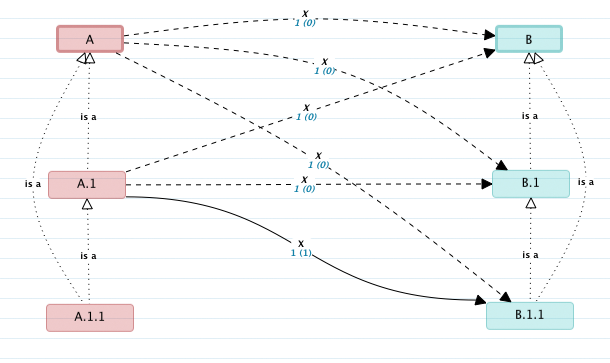
\includegraphics[width=1.0\linewidth]{Figures/proposed_relations1.png}
  \caption[APIUA: Modellierung --- Hypothetische Relationen I]{Die Relation \rel[x]{\code{apiua://code/-9223372036854774934}}{\code{apiua://code/-9223372036854774931}} ist in diesem ACM die einzige explizite Relation. Die übrigen mit gestrichelten Kanten dargestellten Relationen sind Vorschläge, die sich aus \rel[x]{\code{apiua://code/-9223372036854774934}}{\code{apiua://code/-9223372036854774931}} ergeben.}
  \label{fig:ProposedRelations1}
\end{figure}

\begin{figure}
  \centering
    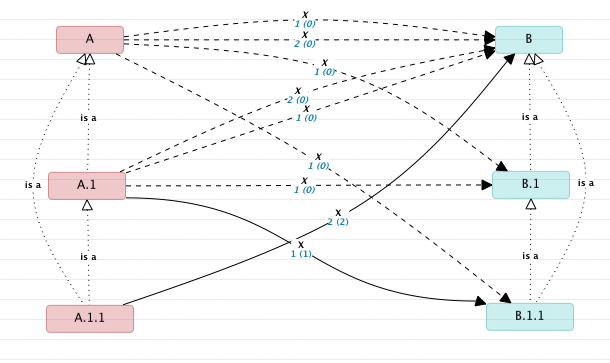
\includegraphics[width=1.0\linewidth]{Figures/proposed_relations2.png}
  \caption[APIUA: Modellierung --- Hypothetische Relationen II]{Dieses ACM unterscheidet sich von \ref{fig:ProposedRelations1} lediglich darin, dass es neben \rel[x]{\code{apiua://code/-9223372036854774934}}{\code{apiua://code/-9223372036854774931}} auch die Relation \rel[x]{\code{apiua://code/-9223372036854774932}}{\code{apiua://code/-9223372036854774935}} enthält. Daraus ergeben sich mehrere gleich lautende hypothetische Relationen zwischen denselben Konzepten (insb. zwischen \code{apiua://code/-9223372036854774936}~und~\code{apiua://code/-9223372036854774935}).}
  \label{fig:ProposedRelations2}
\end{figure}

\begin{figure}
  \centering
    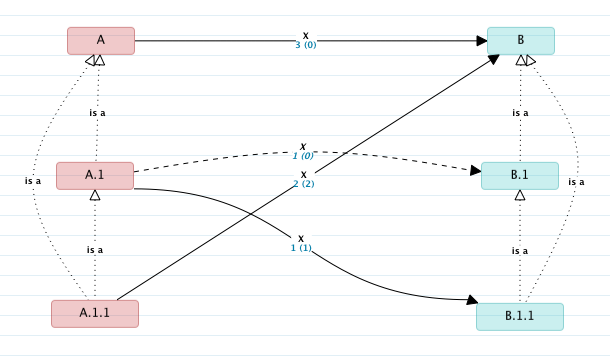
\includegraphics[width=1.0\linewidth]{Figures/proposed_relations3.png}
  \caption[APIUA: Modellierung --- Hypothetische Relationen III]{Im Gegensatz zu \ref{fig:ProposedRelations2} enthält dieses ACM zwischen \code{apiua://code/-9223372036854774936} und \code{apiua://code/-9223372036854774935} die explizite Relation \rel[x]{\code{apiua://code/-9223372036854774936}}{\code{apiua://code/-9223372036854774935}}. Dadurch entfallen alle hypothetischen Relationen, die in \code{apiua://code/-9223372036854774936} oder \code{apiua://code/-9223372036854774935} anfangen oder enden. Die einzig erhalten gebliebene hypothetische Relation ergibt sich aus \rel[x]{\code{apiua://code/-9223372036854774934}}{\code{apiua://code/-9223372036854774931}}.}
  \label{fig:ProposedRelations3}
\end{figure}

Informatisch gesehen ist das Produkt der Analyse, das hauptsächlich in den Phasen des offenen und axialen Kodierens entsteht, eine Ontologie --- also eine ``explizite Spezifikation einer Konzeptualisierung'' \citep{Gruber:1993jz}. Denn: Bevor der Forscher seine \acrlong{gt} in Form einer so genannten \textit{Story} erzählt, liegen lediglich \glspl{acm} vor, die man durch eine Ontologie beschreiben kann. Man könnte also auch vereinfacht(!) sagen, dass eine \acrlong{gt} auf einer rückwärts mit Hilfe synthetischen Schließens entwickelten Ontologie basiert, die in den Daten verankert ist bzw. ein Model für die Daten darstellt. Meiner Meinung nach eignet sich diese Beobachtung dazu, bessere Datenanalysewerkzeuge zu entwickeln, als es sie heute gibt.

Wenn man einmal von den im \sref{sec:gtm} angesprochenen terminologischen Ungereimtheiten der \gls{gtm} absieht, gibt es einen abgegrenzten Baukasten von Elementen (Konzepte, Eigenschaften, Kategorien, Relationen, etc.), aus denen die Grundlage der \gls{gt} besteht. Diese mögliche Anordnung dieser Elemente könnte man in einer Meta-Ontologie beschreiben. Ein \gls{gtm} geeignetes Datenanalysewerkzeug müsste dann nur noch diese Meta-Ontologie unterstützen und dem Forscher zur Verfügung stellen. Schließlich würde jede Ontologie, die ein Forscher entwickelt, eine Instanz dieser Meta-Ontologie sein.

Trifft man die Annahme, dass jede Theorie gewissen Gesetzmäßigkeiten unterliegt (z.B. Vererbung wie oben beschrieben), könnte man diese Interferenz- und Integritätsregeln ebenfalls in der Meta-Ontologie beschreiben. Auf diese Weise könnte ein Datenanalysewerkzeug Verletzungen der Ontologie an der Meta-Ontologie diagnostizieren und implizites Wissen durch Anwendung der Interferenzregeln explizit machen.

In \gls{apiua} sind Interferenzregeln wie hypothetische Relationen aktuell fest kodiert. Ideal wäre es, wenn Interferenzregeln selbst vom Anwender definiert und bedarfsweise, beispielsweise während Erkenntnisperspektivwechseln, (de)aktiviert werden könnten. Auf diese Weise müssten keine Gesetzmäßigkeiten mehr postuliert werden, die für alle Theorien gelten. Stattdessen hätte der Forscher die Möglichkeit, für seine \gls{gt} individuelle Regeln zu formulieren.

Ein ganz konkreter Anwendungsfall für individuelle Interferenzregeln könnte wie folgt lauten: Für fünf von sechs Unterkodes von Kode \code{apiua://code/-9223372036854774936} gilt die Relation \rel{\code{A\textsubscript{x}}}{\code{apiua://code/-9223372036854774935}}. Das Werkzeug könnte nun dem Anwender vorschlagen, zu prüfen, ob diese Relation möglicherweise auch für den sechsten Untercode von \code{apiua://code/-9223372036854774936} zutrifft und damit auf \rel{\code{apiua://code/-9223372036854774936}}{\code{apiua://code/-9223372036854774935}} verallgemeinert werden kann. Das Werkzeug sollte sich darüber hinaus die Grundlage dieser Entscheidung merken. Sollte später ein siebter Unterkode zu \code{apiua://code/-9223372036854774936} hinzukommen, gäbe es zwei Möglichkeiten: (1) Der Forscher prüft selbstständig, ob \rel{\code{apiua://code/-9223372036854774936}}{\code{apiua://code/-9223372036854774935}} auch für \rel{\code{A\textsubscript{7}}}{\code{apiua://code/-9223372036854774935}} gilt. (2) Das Datenanalysewerkzeug erkennt die veränderte Datenlage und fragt den Anwender aktiv. Die zweite Möglichkeit würde eine Umstrukturierungsoperation im Sinne der in \tref{tab:APIUARequirements} aufgezählten Anforderungen darstellen.

Die Krux ist, dass der Forscher im Sinne des \textit{ständigen Vergleichens} und der Güte seiner Forschungsergebnisse  dazu verpflichtet ist, die im Beispiel skizzierten Überlegungen anzustellen. Ich halte es aber für unwahrscheinlich, dass der Forscher diesem Anspruch bei hinreichend komplexen Abhängigkeiten innerhalb seiner Theorie ohne Werkzeugunterstützung genügen kann.

Diese von mir vorgeschlagenen Verbesserungen sind allerdings mit Vorsicht zu genießen, denn sie sind nicht ausgiebig erprobt. Im Rahmen der in dieser Arbeit präsentierten Forschung haben die implementierten Funktionen (Vererbung von Verankerungen; hypothetische Relationen; siehe \sref{sec:Datenanalyse-STL-Inkonsistenzen-vereinfachen}) zwar das axiale Kodieren deutlich vereinfacht. Dennoch kann man zu bedenken geben, dass allein der von einem Werkzeug stammende Vorschlag zur Änderung des eigenen Theoriemodells den Anwender auf eine Weise beeinflusst, auf die er ohne diese Hilfestellung nicht beeinflusst worden wäre. Ich kann nicht ausschließen, dass der unreflektierte Umgang mit derartigen Funktionen zu einer gewissen Starrheit/Rigidität auf Seiten des Forschers führen kann.

Meine ontologische Auseinandersetzung mit der \gls{gtm} an dieser Stelle war vornehmlich technisch gemeint. Sie möchte zum einen die Möglichkeit geben --- insbesondere im Rahmen von Open Science  --- Forschungsergebnisse menschen- aber auch maschinenlesbar zur Verfügung zu stellen. Das Potential dieses Vorgehens stellt auch \cite{MuhlmeyerMentzel:2011vs} heraus. Zum anderen möchte sie als Vorschlag für den Bau einer besseren Datenanalysesoftware verstanden werden. Die Abschätzung der Konsequenzen für eine derart entwickelte \gls{gt} kann diese Arbeit nicht leisten. Allein das Feld der \acrlong{gtm} mit seinen verschiedenen Strömungen \citep{Breckenridge:2012tf}, wie der klassischen \gls{gtm} von \cite{glaser1978theoretical}, der von \cite{strauss1990basics} oder der konstruktivistischen \gls{gtm} von \cite{charmaz2006constructing} ist dafür zu breit.



\subsection{Zusammenfassung}

In diesem Unterkapitel habe ich das für meine Forschung entwickelte Datenanalysewerkzeugs \gls{apiua} vorgestellt.

Qualitative Datenanalysewerkzeuge müssen große Datenmengen, verschiedenste Datenformate und alle Phasen bzw. Praktiken der \gls{gtm} unterstützen, um eine \gls{gt} von hoher Qualität nicht zu gefährden. Um einen wirklichen Mehrwert zu erzielen, müssen ebenso Umstrukturierungsoperationen und Analysefunktionen angeboten werden. Die Interoperabilität der Forschungsergebnisse erlaubt die Weiterverarbeitung durch andere Akteure der Forschungsgemeinde. 

\gls{apiua} verwendet zur Erfüllung dieser Anforderungen eine komponentenbasierte Drei-Ebenen-Architektur. Komponenten werden durch den Einsatz der \gls{rcp}, welche wiederum auf \gls{osgi} basiert, unterstützt. Das Werkzeug ist allgemein, aber insbesondere mit Hinblick auf die Unterstützung weiterer Datenformate, außerordentlich erweiterbar. Die \gls{gtm}-Komponente arbeitet ausschließlich mit \glspl{uri}, durch die jeder Datenpunkt eindeutig identifiziert wird. Auf diese Weise werden Funktionen wie das Kodieren von Daten oder das Schreiben von Memos einheitlich implementiert. Außerdem ist so das Werkzeug bei der Erfüllung der Gütekriterien \textit{Argumentative Interpretationsabsicherung} und \textit{Nähe zum Gegenstand} behilflich. 

\gls{apiua} erlaubt die Arbeit mit hoch strukturierten Daten. Die Anwendung wurde mit dem Anspruch entwickelt, selbst benutzerfreundlich zu sein. Dazu gehört unter anderem eine frei konfigurierbare Benutzeroberfläche, die ihren Zustand detailliert über mehrere Forschungssitzungen speichert und nicht --- im Gegensatz zu anderen Werkzeugen --- immer wieder neu hergestellt werden muss.

Im Unterschied zu \textit{ATLAS.ti} können in \gls{apiua} Kodes einfach gefiltert, intuitiv farbkodiert, sortiert und hierarchisch angeordnet werden. Trotz der überschaubaren Funktionalität wird axiales Kodieren in \gls{apiua} in einem konkurrenzlosen Umfang unterstützt.

Das Werkzeug unterstützt fest implementierte Interferenzregeln, die besonders beim axialen Kodieren hilfreich sind und bei \textit{ATLAS.ti} in keiner Weise angeboten werden. Eine Möglichkeit, frei konfigurierbare Interferenzregeln zu erlauben, erachte ich für außerordentlich wünschenswert. Eine Möglichkeit, dies zu erlauben, besteht darin, mit einer Meta-Ontologie zu arbeiten. Ich biete die Grundlage, auf der die zukünftige Forschung meine Überlegungen untersuchen kann.

Abgesehen vom Umbenennen unterstützt \textit{ATLAS.ti} keinerlei Umstrukturierungsoperationen. In der aktuellen Version bietet \gls{apiua} jedoch einige Funktionen, wie Operationen am Kodebaum und die Verallgemeinerung bzw. Zusammenfassung von Relationen. Umstrukturierungsfunktionen wie das Zusammenfassen oder Auftrennen von Kodes fehlen beiden Werkzeugen.

Weitergehende Analysefunktionen fehlen beiden Anwendungen ebenfalls. Eine Funktion zum Anzeigen von Kodes, die nur in wenigen Datenquellen auftauchen, wäre außerordentlich spannend. Mit dieser Information könnte der Forscher beispielsweise \textit{theoretisches Sampling} besser betreiben --- also exakter auswählen ob und welche Daten er noch erheben möchte, was wiederum der Erfüllung des Gütekriteriums \textit{Triangulierung} zuträglich wäre.

%Im \hyperref[sec:ausblick]{Ausblick} greife ich noch einmal die wichtigsten Punkte auf.

\bigskip

Der nächste Abschnitt befasst sich mit der eigentlichen \gls{gtm}-Analyse unter Verwendung des eben beschriebenen qualitativen Datenanalysewerkzeugs \acrlong{apiua}.
\section[Phase 4: Durchführung der GTM-Datenanalyse]{Phase 4: Verfahren der Analyse der API-Usability von SeqAn mit Hilfe der Methode der Grounded Theory}
\label{sec:phase4}

Wie bereits mehrfach --- insbesondere in den Abschnitten \ref{sec:gtm} und \ref{sec:verlauf} --- erläutert, habe ich für meine Forschung die \acrfull{gtm} eingesetzt. Dazu habe ich ein spezielles Datenerhebungsverfahren (siehe \sref{sec:phase2}) und ein dazu passendes Datenanalysewerkzeug (siehe \sref{sec:apiua}) entwickelt.

Speziell zum Zweck der \gls{gtm}-basierten Analyse habe ich die Programmierfortschritte von SeqAn-Anwendern erhoben, eine Gruppendiskussion geführt und einen speziell für die Evaluation von APIs entwickelten Cognitive-Dimensions-Fragebogen eingesetzt.
\\Darüber hinaus habe ich die Ergebnisse aus der Beseitigung grober Usability-Probleme (siehe \sref{sec:phase1}) in meine Analyse einbezogen. Zur Erinnerung: Für diese erste Phase kamen eine \acrfull{he} und drei Befragungen (Online-Umfrage, Interviews, Feedback-Zettel) zum Einsatz.

In dieser Phase stelle ich zunächst die Forschungsmethoden anderer Studien vor. Anschließend erläutere ich den Verlauf meiner Forschung an Hand der verschiedenen in der vorherigen Phase erhobenen Daten. Meine Probleme bei der Anwendung der \gls{gtm} bespreche ich im darauffolgenden Abschnitt. Abschließend demonstriere ich anekdotisch und an konkreten Beispielen meine Forschungsgründlichkeit bevor ich im nächsten Kapitel meine Forschungsergebnisse vorstelle. 

\subsection{Vergleich mit anderen Studien}

Die GTM eignet sich besonders gut für die explorative Erforschung schlecht erforschter Gegenstandsbereiche \citep{mayring2002einfhrung}. Es handelt sich dabei um einen empirischen Forschungsansatz, dessen Nutzen für die Untersuchung von API-Usability bereits beschrieben wurde \citep{SIGCHI:2009up}. Bereits \cite{Brooks:1980kb} hat die Notwendigkeit erkannt, API-Nutzungsdaten qualitativ und datenverankert zu analysieren und zu interpretieren.

Die Kombination verschiedener Evaluationsmethoden (in dieser Arbeit: \gls{he} und \gls{gtm}) unter Verwendung unterschiedlicher Datenquellen, stellt ein Gütekriterium im Sinne der \textit{Triangulierung} \citep[siehe \sref{sec:gtm} und][]{mayring2002einfhrung} dar und hat sich bereits mehrfach als geeignetes Mittel zur Erlangung eines reichhaltigen Verständnisses bewährt \citep{Boehm:2003tc,Grill:2012jm}. Hingegen kann der alleinige Gebrauch von klassischen Usability-Evaluationsverfahren (siehe \sref{sec:literatur-klassische-usability-evaluation}) die Interaktion zwischen API und API-Anwendern nur teilweise erfassen \citep{Tenny:2011jp}. Die Nutzung von Erkenntnissen aus anderen Disziplinen wurde bereits von \cite{BenShneiderman:gn} gefordert --- umso erstaunlicher, dass diesem Ruf die Forschergemeinde kaum nachkam \citep{Glass:2002ec}.

Empirische Verfahren erlauben sehr tiefe Einsichten, skalieren aber schlecht und werden von \cite{SIGCHI:2009up} nur zur Evaluation eines einzelnen API-Features für geeignet betrachtet (siehe \fref{fig:api-usability-granularitaet}).

\begin{figure}
  \centering
    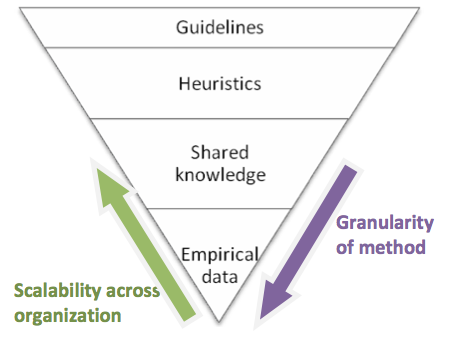
\includegraphics[width=0.5\linewidth]{Figures/api-usability-granularitaet.png}
  \caption{Skalierbarkeit von API-Evaluationsverfahren \citep{SIGCHI:2009up}}
  \label{fig:api-usability-granularitaet}
\end{figure}

Meine Arbeit ist nicht die einzige, bei der der eigentlichen Forschung eine \gls{he} vorausging. Eine andere Arbeit \citep[siehe \sref{sec:grill} und ][]{Grill:2012jm} nutzt diesen Ansatz auch --- jedoch nicht, um den Untersuchungsgegenstand für die Forschung vorzubereiten, sondern um vorab zu ermitteln, worauf sich die anschließende Erforschung fokussieren sollte. Die von mir durchgeführte \gls{he} diente jedoch lediglich der Beseitigung grober Usability-Probleme und der nicht-einschränkenden Sensibilisierung für mögliche Probleme.

Die Methode \textit{Concept Maps} \citep[siehe \sref{sec:concept-maps} und][]{Tenny:2011jp} hat sich ebenfalls als geeignet für die explorative Erforschung einer API herausgestellt. Jedoch setzt sie eine sehr hohe Einbeziehung der API-Entwickler voraus, was sich angesichts des im \sref{sec:schwierigkeiten} geschilderten \textit{technischen Wegargumentierens} \citep{Sarodnick:2006vc} als nachteilig herausgestellt haben könnte.

Das \textit{Cognitive Dimensions Framework} wird in der Forschung von \cite{clarke:2006} zur API-Usability-Evaluation eingesetzt. Wie ich bereits im \sref{sec:api-cds} beschrieben habe, ist die Darstellung des Verfahrens in der Literatur mangelhaft, was sich aber leider erst beim Versuch seiner Anwendung herausgestellt hat. Auch der Versuch, eine kostengünstige Validierung meiner im nächsten Kapitel dargestellten Forschungsergebnisse durchzuführen, ist gescheitert. Dieser Validierungsversuch wird am Ende des nächsten Kapitels (siehe \sref{sec:cdf-validation-difficulties}) erläutert.

In einer Studie zur Verbesserung einer Persistenz-Bibliothek \citep[siehe \sref{sec:piccioni} und][]{Piccioni:2013uq} wurden die kognitiven Dimensionen für APIs von \cite{Anonymous:9HSMlhmF} für die Vorbereitung von Interviewfragen genutzt. Leider ist die Zustandekommen fraglich, weil es nicht nachvollziehbar dargestellt wurde (siehe \sref{sec:cdf-usage}).

Wie bereits am Anfang dieser Arbeit gezeigt (siehe \sref{sec:gtm-informatik}), wurde die \gls{gtm} nur in drei mir bekannten und lediglich mittelbar für API-Usability-Forschung relevanten Studien \citep{Simula.simula.1294,Yamashita:2013hn,Yamashita:2013un} korrekt eingesetzt. Dabei kamen ``lediglich'' die Phasen \textit{offenes Kodieren} und \textit{axiales Kodieren} zum Einsatz. In der unmittelbar relevanten API-Usability-Forschung setzten \cite{Tenny:2011jp,deSouza:2004fd,sunshine2014searching} die \gls{gtm} nur geringfügig und mangelhaft bzw. kaum nachvollziehbar ein.


\subsection{Analyse mit Hilfe der Methode der Grounded Theory}
\label{sec:gtm-application}

Wie bereits am Anfang dieses Kapitels (siehe \sref{sec:verlauf}) beschrieben, wich meine Forschung stark von der ursprünglichen Planung ab. Die ohnehin spezielle Art der Datenerhebung und der erhobenen Daten selbst, machte die Entwicklung eines dafür geeigneten qualitativen und \gls{gtm}-unterstützenden Datenanalysewerkzeugs notwendig. Die Datenanalyse und die daraus gewonnen Erkenntnisse standen in ständiger Wechselwirkung mit den Datenerhebungen und der Werkzeugentwicklung. Beispielsweise stellte ich bei der Datenanalyse fest, dass ich nicht sehen konnte, welche Begriffe die SeqAn-Anwender in das Suchfeld der Onlinedokumentation eingegeben hatten, woraufhin ich die Datenerhebung anpassen musste (Details siehe \sref{sec:datenerhebung-probleme}). Wiederum haben die ständigen Verbesserungen von Datenerhebung und Analysewerkzeug Zeit gekostet. Der so entstandene Zeitdruck wirkte sich auf die Analysetiefe, die Auswahl der zu analysierenden Daten und schließlich auch auf die in \hyperref[sec:Ergebnisse]{Kapitel 4 vorgestellten Ergebnisse} aus.

\subsubsection{Analyse der Programmierfortschritte-Daten}

Für den ersten Analyseversuch verwendete ich den \acrfull{apiua} in Verbindung mit den während der Workshops'11 erhobenen Programmierfortschritte-Daten. Die Ergebnisse dieses Versuchs sind in \fref{fig:research-ohne-sensibilisierung} dargestellt. Als damaliger \gls{gtm}- und \acrshort{api}-Usability-Evalations-Anfänger musste ich nach insgesamt etwa drei Monaten feststellen, dass mich meine Forschung nur wenig voran gebracht hatte. Wie die Abbildung zeigt, habe ich die Programmierfortschritte unter verschiedenen Gesichtspunkten --- beispielsweise \code{apiua://code/-9223372036854775741} und \code{apiua://code/-9223372036854775734} --- analysiert.

%\newgeometry{inner=2cm,outer=1.5cm,top=1.5cm,bottom=1.5cm}
%\thispagestyle{empty}
%\begin{landscape}
\begin{figure}
  \centering
    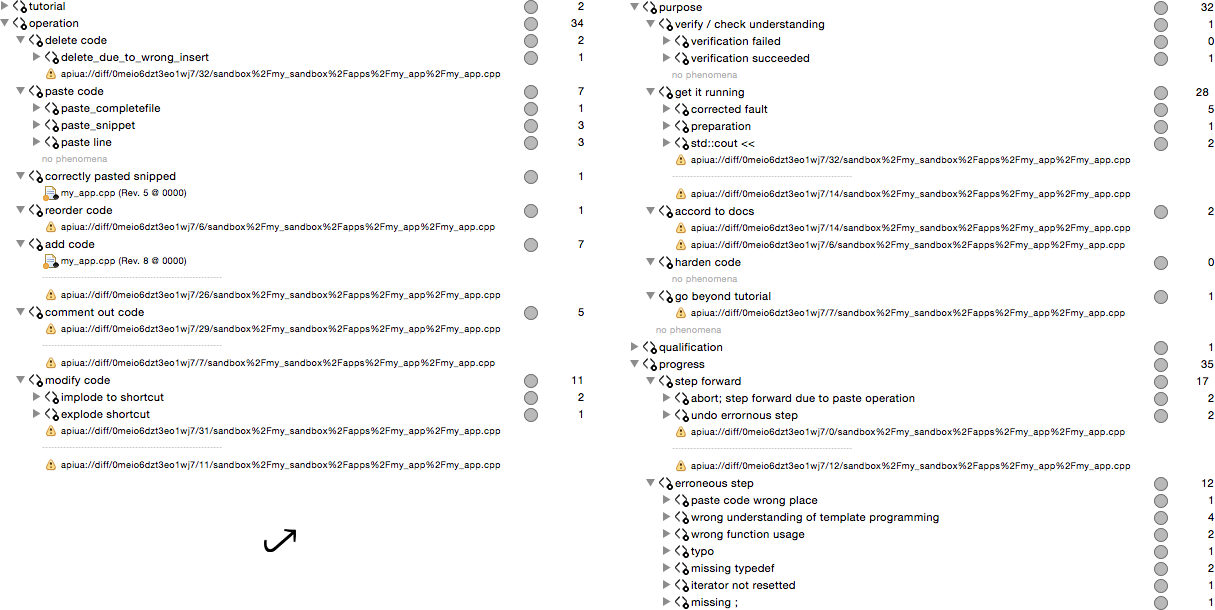
\includegraphics[width=1.0\linewidth]{Figures/research/ohne-sensibilisierung.png}
  \caption[Ergebnisse des ersten Analyseversuchs]{Ergebnisse der ersten Analyseversuchs: Die Abbildung zeigt die hierarchische Kodestruktur die bei dem ersten Versuch einer Analyse entstand. Aus technischen Gründen ist der Baum in zwei Spalten aufgetrennt. Innerhalb einer Spalte gibt es drei Spalten, von denen die erste den Namen des Kodes bzw. deren Phänomene/Verankerungen darstellt. Die grauen Linien geben an, dass aus Darstellungsgründen weite Phänomene ausgeblendet sind. Die tatsächliche Anzahl von Phänomenen steht in der dritten Spalte. Die zweite Spalte gibt die Farben der Kodes. Sie ist hier grau, weil diese Kodes nicht weiter verwendet wurde.}
  \label{fig:research-ohne-sensibilisierung}
\end{figure}
%\end{landscape}
%\restoregeometry

Ganz erkenntnislos war der erste Analyseversuch jedoch nicht. So deuteten die Kodes \code{apiua://code/-9223372036854775739} und \code{apiua://code/-9223372036854775751} bereits auf das Konzept der \code{apiua://code/-9223372036854774904} hin.% (Dem aufmerksamen Leser wird auffallen, dass die beiden Kodes damals noch nicht zusammengefasst wurden.)

Während der Analyse vollzog ich typischerweise die folgenden Schritte, die in \fref{fig:research-workflow-diff} veranschaulicht werden. Die folgenden Schritte beziehen sich auf den Kode \code{apiua://code/-9223372036854775739}:
\begin{enumerate}
  \item Zunächst habe ich einen Proband ausgewählt, dessen Programmierfortschritte ich analysieren wollte. Der entsprechende Anzeigebereich führt alle Probanden an Hand ihrer ID und ihrer Browser-Fingerprints (Details siehe \sref{sec:id}) auf. In diesem Beispiel wurde Proband \textit{0meio6dz3eo1wj7} geöffnet.
  \item Die Programmierfortschritte des Probanden können auf zweierlei Weise erkundet werden.
  \\(2a) zeigt sämtliche Aktionen des Probanden auf einer Zeitleiste:
  \\(2b) beschränkt sich auf die Darstellung der Fortschritte beim Programmieren.
  \\In diesem Beispiel interessierte mich die Datei \texttt{my\_app.cpp} der \textit{Revision 5}, die den fünften Kompilierversuch symbolisiert.
  \item Die Diff-Ansicht stellt die vorangegangene und aktuelle Version der Datei \texttt{my\_app.cpp} gegenüber. Offenbar wurden sehr viele Änderungen vorgenommen. Eine derartige, fehlerfrei wirkende Operation ist für einen SeqAn-Anfänger ungewöhnlich. Dafür musste es also eine Erklärung geben.
  \item Der Bereich (4a) stellt listenartig alle Ereignisse auf der Online-Dokumentation dar. Der Bereich (4b) stellt dieselben Informationen in der untersten Zeile der Zeitleiste dar. Der bläuliche Einfärbung auf der Zeitleiste markiert dabei den Zeitraum des Workshops. Die neongrünliche Einfärbung hebt sämtliche Ereignisse hervor, die in die Zeitspanne der Arbeiten an der fünften Revision der Datei \texttt{my\_app.cpp} fallen.
  \\Bleibt der Forscher mit der Maus über einem Ereignis stehen, werden detaillierte Informationen in (5) dargestellt.
  \item Der Detaildialog ist ein nicht-modales Fenster, wie man es aus der Eclipse-Entwicklungsumgebung, beispielsweise bei der Codevervollständigung kennt. In diesem Fall zeigt das Fenster an, was genau der Proband in diesem Moment auf der Online-Dokumentation gesehen hat. Der blasse Pfeil im Hintergrund des Screenshots bedeutet, dass der Anwender herunter gescrollt ist, um den dargestellten Bereich zu sehen. Der Screenshot zeigt ein SeqAn-Online-Tutorial. Durch den Vergleich des Tutorial-Inhalts mit dem, was der Anwender programmiert hat, wird deutlich, dass er zwei Code-Fragmente aus dem Tutorial kopiert und in seiner C{}\verb$++$-Datei eingefügt hat.
  \item Die beiden Fragmente habe ich mit dem Kode \code{apiua://code/-9223372036854775739} kodiert. Da die Kodeansicht alle existierenden Kodes darstellt, bietet es sich an dieser Stelle an, die Kodierung mit den bereits kodierte Phänomenen im Sinne des \textit{ständiges Vergleichens} gegenüberzustellen, um zu klären, ob es sich wirklich noch um die Semantik des Kodes handelt.
  \item Erkenntnisse können in der Memoansicht festgehalten werden. In diesem Fall war das Memo bereits in Kode \code[apiua://code/-9223372036854775750]{paste\_snippet} festgehalten, der mit \code{apiua://code/-9223372036854775739} zusammengefasst werden sollte.
  \item Die Kodierung der fünften Revision der Datei \texttt{my\_app.cpp} ist abgeschlossen. Die Programmierfortschritte-Ansicht kann nun verwendet werden, um die sechste Revision zu kodieren.
\end{enumerate}

\newgeometry{inner=2cm,outer=1.5cm,top=1.5cm,bottom=1.5cm}
\thispagestyle{empty}
\begin{landscape}
\begin{figure}
  \centering
    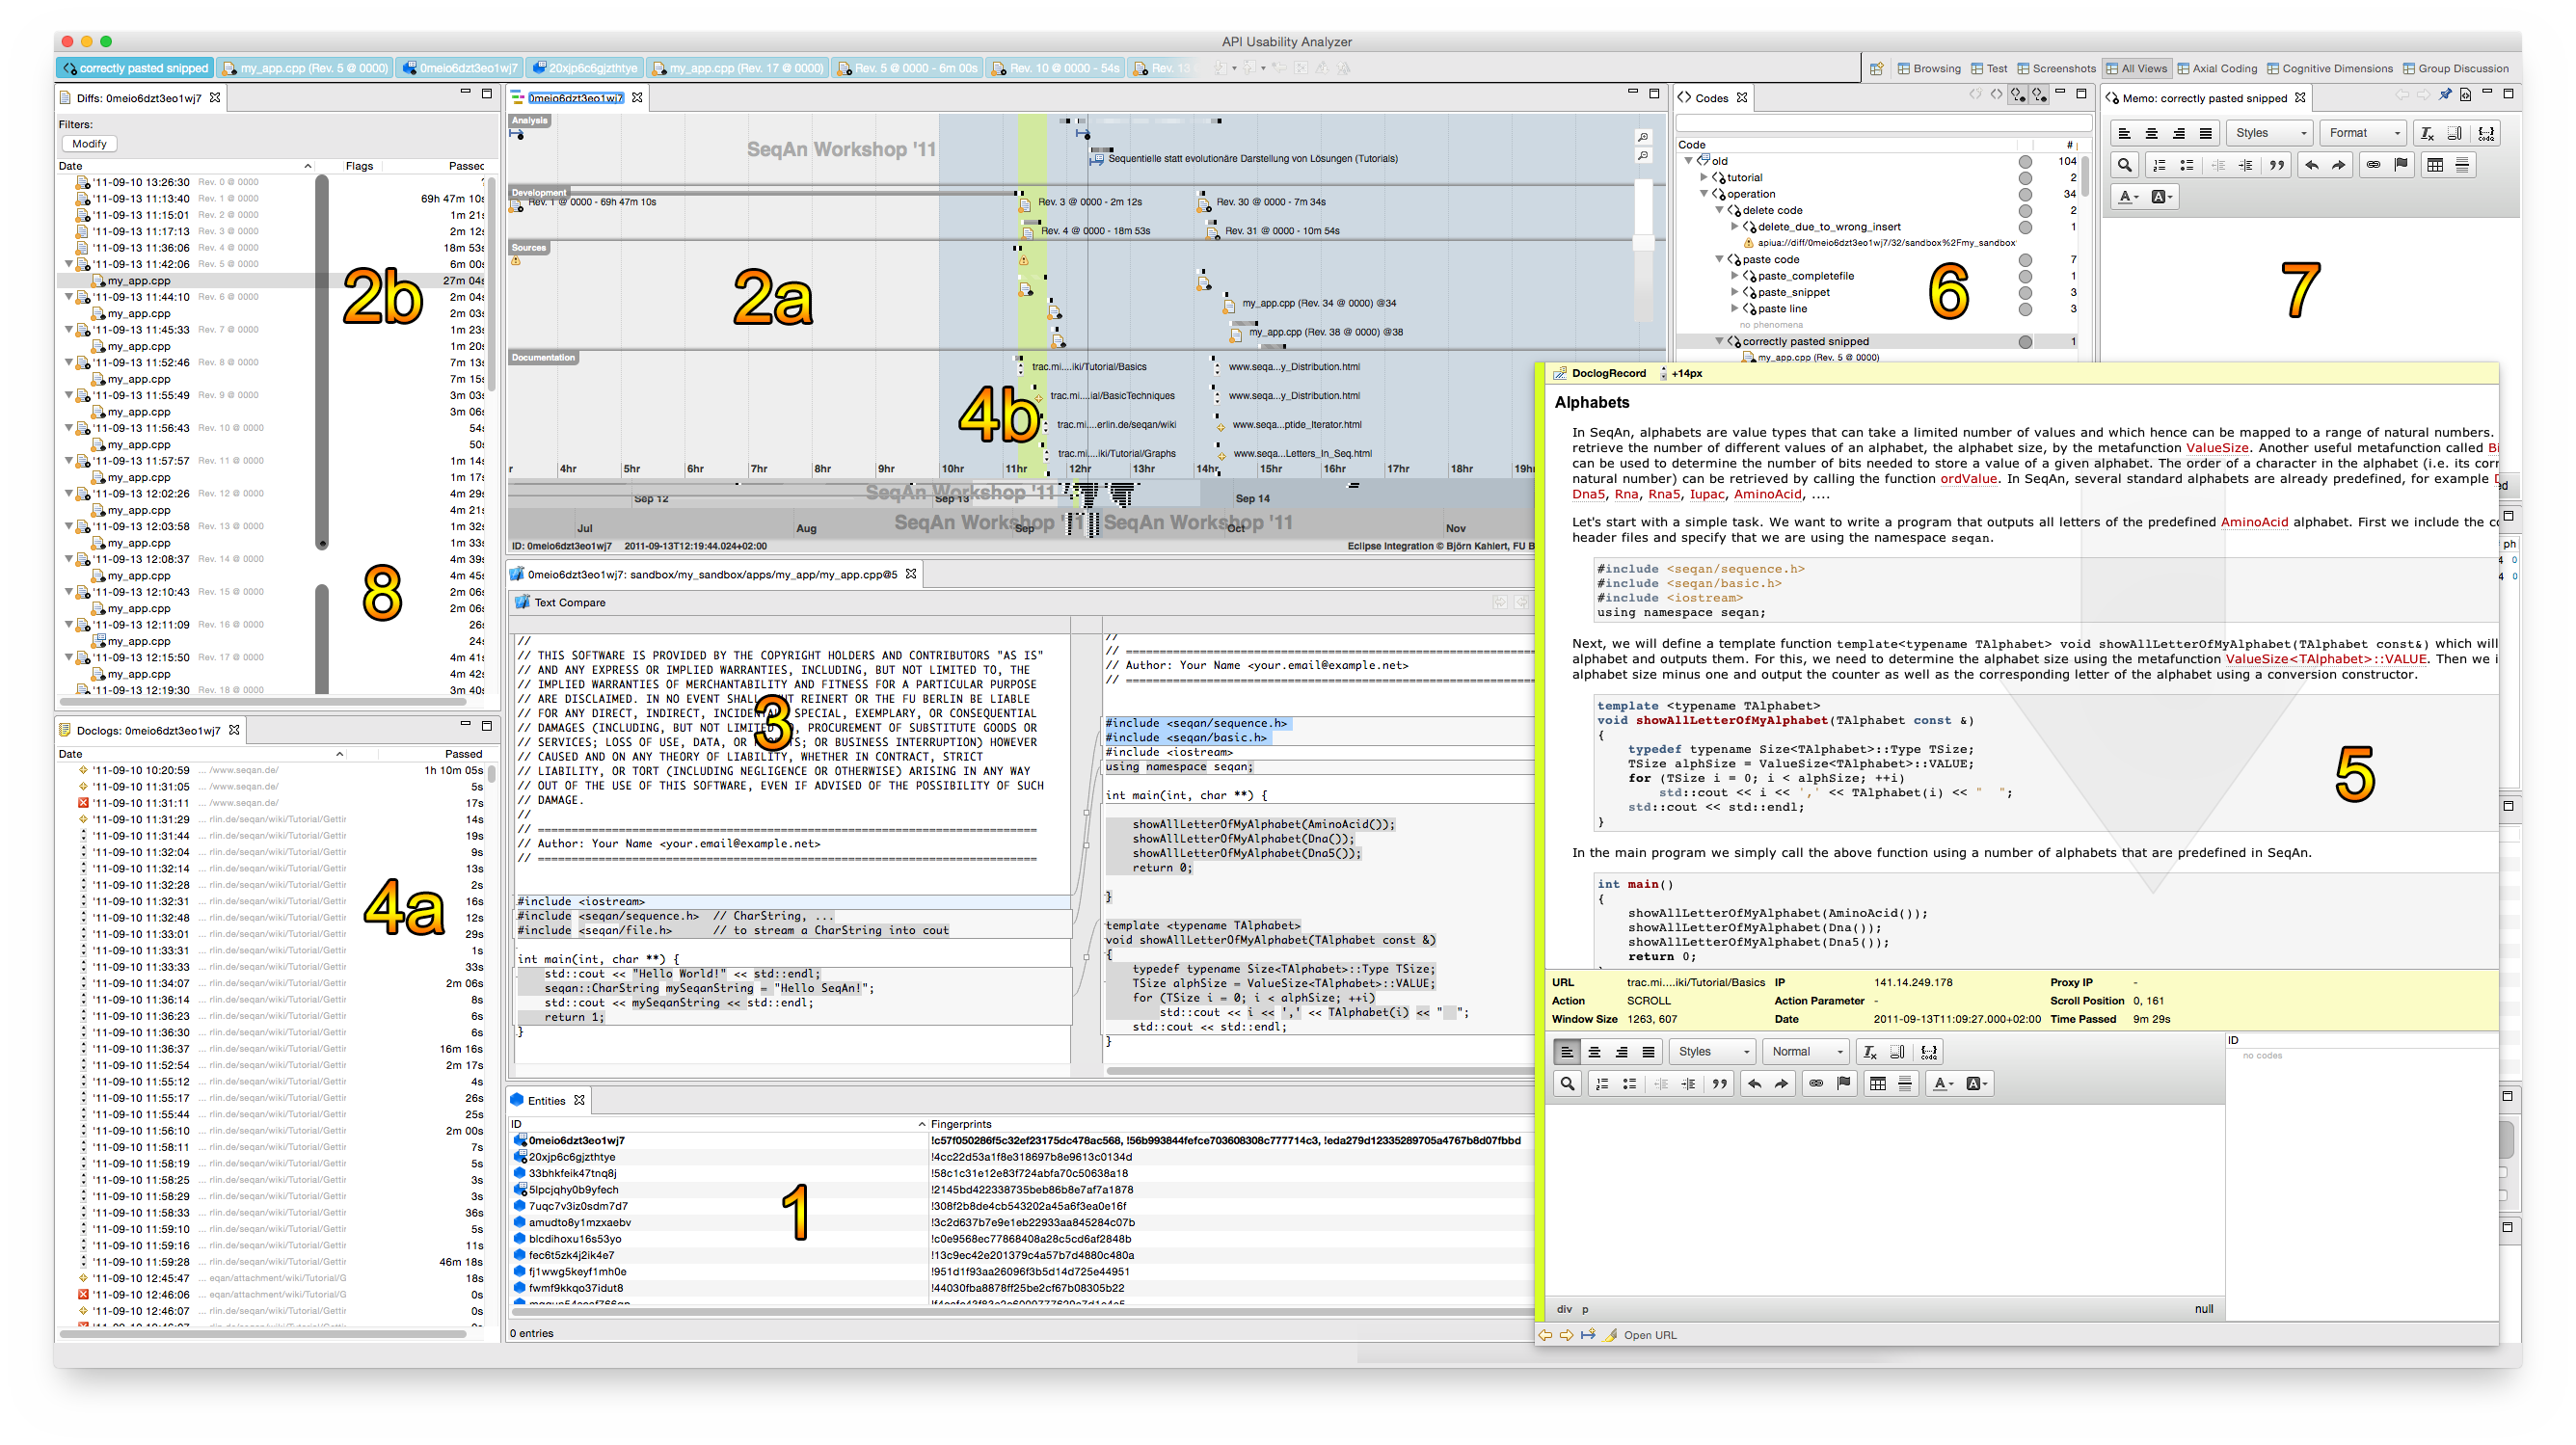
\includegraphics[width=1.0\linewidth]{Figures/research/workflow-diff.png}
  \caption[Analyse von Programmierfortschritte-Daten mit Hilfe von APIUA]{Analyse von Programmierfortschritte-Daten mit Hilfe von APIUA: (1) Auswahl des Probanden, dessen Programmierfortschritte analysiert werden sollen. (2a) zeigt die Programmierfortschritte entlang einer Zeitleiste. (2b) beschränkt sich auf eine Listendarstellung. (3) stellt die vorangegangene und aktuelle Version der selektierten Datei gegenüber. (4a) stellt listenartig alle Ereignisse auf der Online-Dokumentation dar. (4b) Dasselbe macht unterste Zeile der Zeitleiste. (5) stellt detaillierte Informationen zu einem Datenpunkt dar. (6) zeigt die existierenden Kodes. In (7) werden Erkenntnisse zum aktuell selektierten Element festgehalten. Wurde die betrachtete Datei kodiert, kann der Forscher in (8) fortfahren.}
  \label{fig:research-workflow-diff}
\end{figure}
\end{landscape}
\restoregeometry


Auch wenn man auf diese Weise sehr gründliche Analysen durchführen kann, erfordert es viel Übung, ein gewisses Abstraktionsniveau zu erreichen, welches dem selbst gesteckten Ziel genügt. In meinem Fall war dies die Erforschung und insbesondere die Verbesserung der API-Usability von SeqAn.

Um meine Sensibilität zu erhöhen und eine effizientere, gezieltere Analyse der objektiven Programmierfortschritte-Daten zu erreichen, habe ich mich entschlossen, zunächst mit der Analysen der subjektiven Datenquellen \textit{Cognitive-Dimensions-Fragebogen} und \textit{Gruppendiskussion} fortzufahren. Immerhin konnten die Forscher der API-Usability-Studie von \cite{Grill:2012jm} 55\% der entdeckten Usability-Probleme in der direkten Interaktion mit Benutzern (insb. Interviews) finden.



\subsubsection{Analyse der Cognitive-Dimensions-Fragebögen}

Die im \sref{sec:cdf-usage} vorgestellten Cognitive-Dimensions-Fragebögen kamen am Ende des Workshops'13 zum Einsatz. \fref{fig:research-workflow-cdf} zeigt, wie die entsprechende Analyseansicht in \gls{apiua} aussieht. Der Kodierprozess ist dem im vorangegangenen Abschnitt ähnlich genug, um ihn an dieser Stelle kein zweites Mal zu erläutern.

\begin{figure}
  \centering
    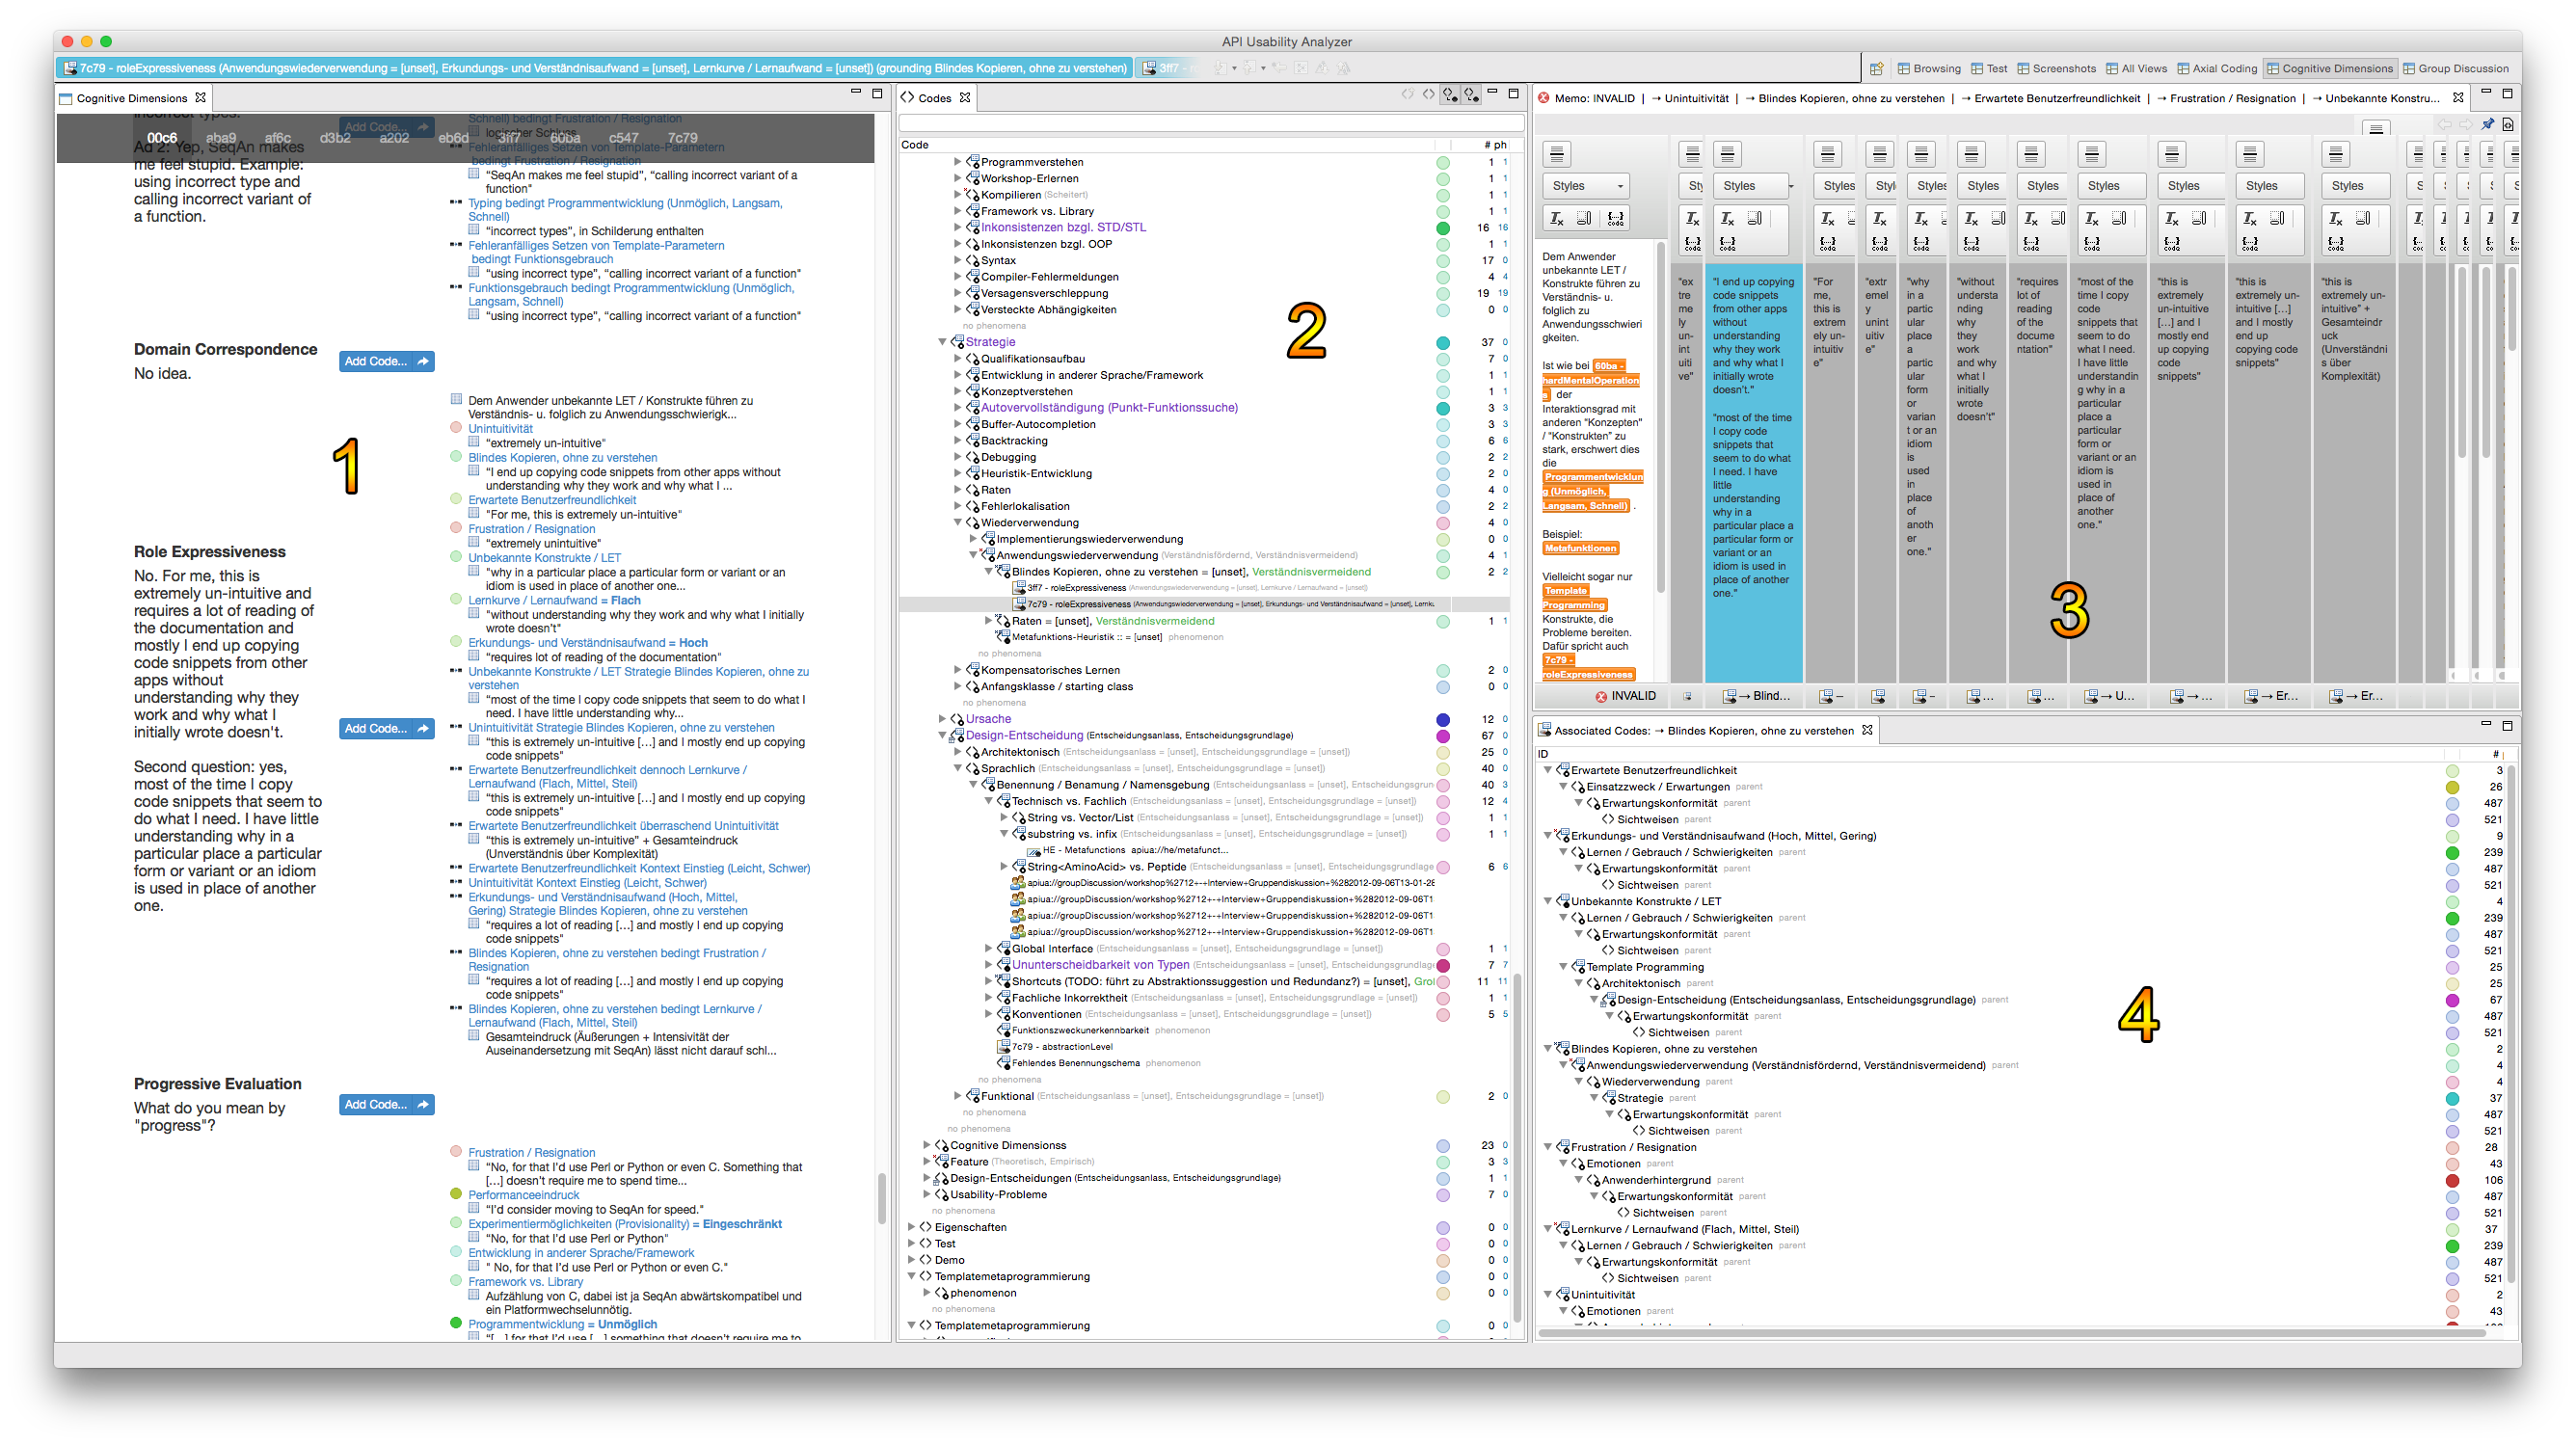
\includegraphics[width=1.0\linewidth]{Figures/research/workflow-cdf.png}
  \caption[Analyse der Cognitive-Dimensions-Fragebögen mit Hilfe von APIUA]{Analyse der Cognitive-Dimensions-Fragebögen mit Hilfe von APIUA: (1) Dieser Bereich stellt alle Antworten der Fragebögen dar. (2) zeigt alle gefundenen Kodes. Neben einem Kode ist dessen Dimensionalisierung dargestellt. Unterhalb eines Kodes sind die Fundstellen/Phänomene aufgelistet. (3) stellt das Memo des aktuell selektierten Elements (blau hervorgehoben), das Memo des zur Selektion gehörenden Kodes (weiß) und die Memos der anderen dem Phänomen zugewiesenen Kodes (grau) dar. (4) listet die zugewiesenen Kodes und deren Elternkode-Hierarchie auf.}
  \label{fig:research-workflow-cdf}
\end{figure}

Die Analyse der Fragebögen war weitaus ergiebiger, auch wenn sie mehrere Monate umfasste. In keiner Datenquelle fand ich so viele Informationen zur Kategorie \code{apiua://code/-9223372036854775237} (u.a. \code{apiua://code/-9223372036854775280} und \code{apiua://code/-9223372036854775279}, siehe \pageref{sec:gt-funktionsbezogene-probleme}) wie in dieser.

An das Beispiel der \code{apiua://code/-9223372036854774904} anknüpfend, konnte ich bei der Analyse der Fragebögen den Kode \code{apiua://code/-9223372036854775508} entdecken. Ein solcher Bezeichner klingt zunächst nach einer mutigen Behauptung, die mit den Programmierfortschritte-Daten --- ohne entsprechende Übung --- nicht einfach zu belegen wäre. In dieser subjektiven Datenquelle fiel das deutlich leichter. So hat beispielsweise ein Proband zu der Frage zur CD \textit{Rolenerkennbarkeit} gesagt: ``[Writing code] is extremely un-intuitive [\dots] and mostly I end up copying code snippets from other apps without understanding why they work''\citepurl{apiua://survey/cd/2013-09-19T11:51:16.616+02:00/domainCorrespondence}.

Manche Fragen wurden von Teilnehmer nicht so verstanden, wie ich das beabsichtigte (Details siehe \sref{sec:cdf-usage}
). Das stellt zwar Forscher vor ein Problem, wenn sie den Fragebogen im Sinne des Cognitive Dimensions Frameworks (siehe Abschnitte \ref{sec:cdf} und \ref{sec:api-cds}) auswerten wollen. Für die \gls{gtm}-Analyse ist dies jedoch unproblematisch, geben die Befragten ja dennoch relevante und wertvolle Informationen.

Bis eben habe ich mich lediglich auf das \textit{offene Kodieren} beschränkt. Für das \textit{axiale Kodieren} waren die Fragebögen weniger geeignet, denn ihnen fehlt weitgehend der Prozesscharakter, der in den Programmierfortschritte-Daten inherent vorhanden ist. Bei den Fragebögen haben die meisten Antworten einen resümierenden, momentbezogenen Charakter, was axiales Kodieren im Sinne des \textit{paradigmatischen Modells} (siehe \sref{sec:gtm}) erschwert. Viele meiner erarbeiteten \textit{\glslink{ac}{axialen Kodierungen}} geben daher auch eher ein Résumé bzw. einen Kausalitätsgraphen wieder. \fref{fig:research-cdf-eb6d} zeigt ein entsprechendes einfaches Beispiel.

\begin{figure}
\begin{minipage}{\textwidth}
  \centering
    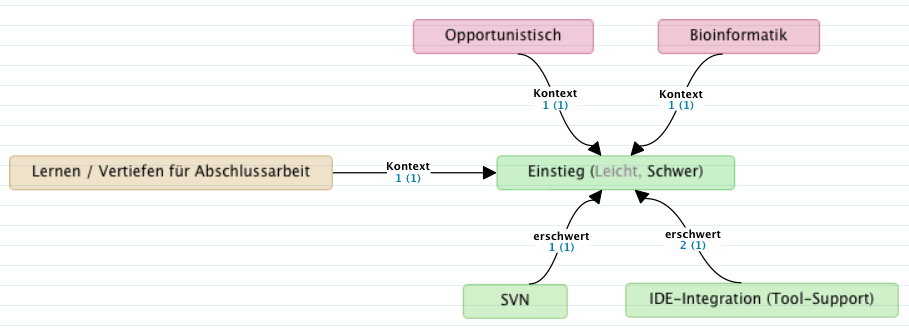
\includegraphics[width=0.75\linewidth]{Figures/research/cdf-eb6d.png}
  \caption[Kausale axiale Kodierung]{Einfache kausale axiale Kodierung\citepurl{apiua://axialcodingmodel/KfDWvbBWybMDxf5O} eines Teilnehmers\citepurl{apiua://survey/cd/2013-09-18T17:46:05.890+02:00}}
  \label{fig:research-cdf-eb6d}
\end{minipage}
\end{figure}

In \fref{fig:research-workflow-cdf} (Bereich 2) kann man bereits erahnen, wie erkenntnisreich die zehn analysierten Fragebögen waren. Ich entschloss mich also, mit der Analyse der zweiten subjektiven Datenquelle \textit{Gruppendiskussion} fortzufahren.



\subsubsection{Analyse der Gruppendiskussion}

In der im \sref{sec:gruppendiskussion} vorgestellten und beim Workshop'12 durchgeführten Gruppendiskussion verwendete ich das Programmierparadigma \textit{Templatemetaprogrammierung} als Hauptreiz. Weitere Reizargumente habe ich hauptsächlich auf der Grundlage von zuvor ausgegebenen Feedback-Zetteln erarbeitet (Details siehe \sref{sec:gruppendiskussion}).

Neben den zu beobachtenden Wiederverwendungsstrategien gaben die Cognitive-Dimensions-Fragebögen umfangreich Aufschluss über unterschiedliche Facetten zur, in SeqAn verwendeten \code{apiua://code/-9223372036854775515}. Ein zuvor unentdeckter Aspekt sind \code[apiua://code/-9223372036854775633]{Inkonsistenzen bzgl. STL} (\textit{STL} steht für die \textit{C}\verb$++$ \textit{Standard Template Library}\footnote{Diese Bezeichnung ist eigentlich nicht ganz korrekt, denn die Standard Template Library (ohne~C++) ist eine von Alexander Stepanov entwickelte Softwarebibliothek für generische Programmierung \citep{TheStandardTemplat:1994vd}, die 1998 in die C++ Standard Library aufgenommen wurde (ISO/IEC 14882:1998).}), die einen Schwerpunkt der Diskussion selbst und meiner mehrmonatigen Analyse darstellte. Die gewonnenen Erkenntnisse sind ein zentraler Punkt meiner im nächsten Kapitel vorgestellten \gls{gt}, weshalb ich an dieser Stelle nicht weiter darauf eingehe.

\fref{fig:research-workflow-gd} zeigt die \gls{apiua}-Perspektive zur Analyse von Gruppendiskussion und veranschaulicht meine Arbeitsweise mit dem \gls{apiua}-Werkzeug.

\begin{figure}
\begin{minipage}{\textwidth}
  \centering
    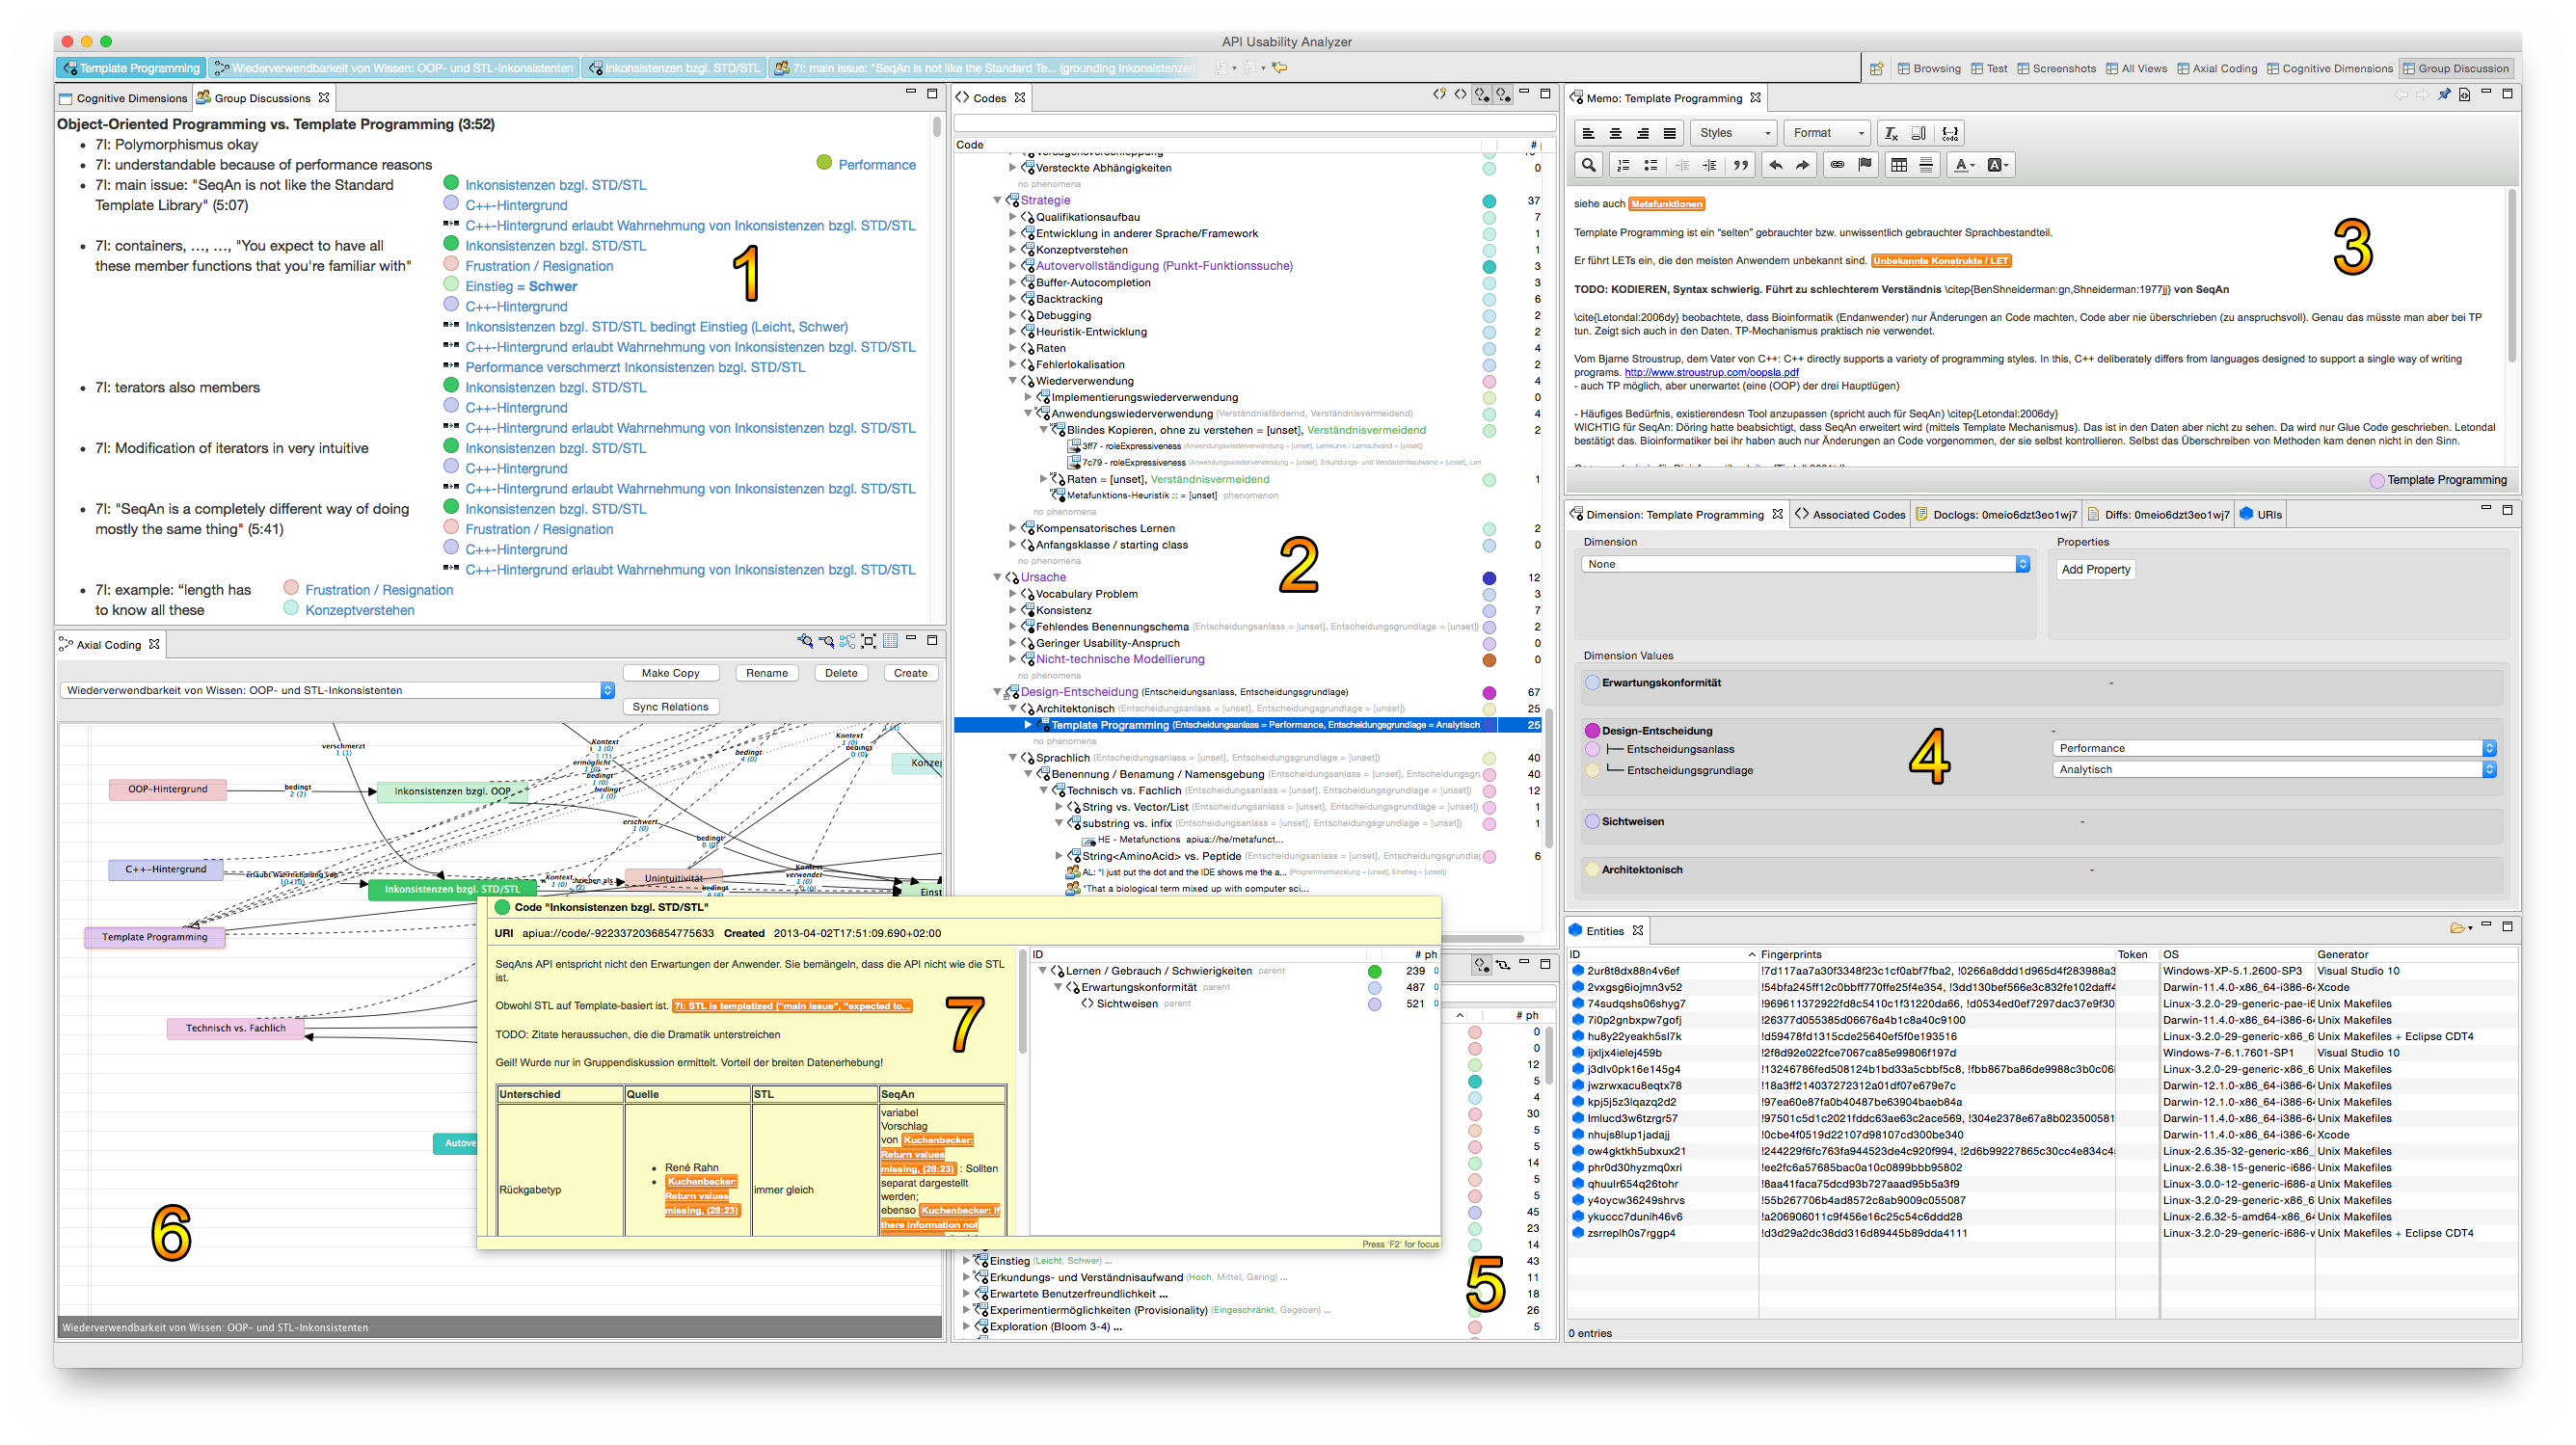
\includegraphics[width=1.0\linewidth]{Figures/research/workflow-gd.png}
  \caption[Analyse der Gruppendiskussion mit Hilfe von APIUA]{Analyse der Gruppendiskussion mit Hilfe von APIUA: (1) zeigt das informelle Transkript der Gruppendiskussion. (2) zeigt die gefundenen Konzepte. (3) zeigt das Memo zur \code{apiua://code/-9223372036854775515}. (4) zeigt die von \code{apiua://code/-9223372036854775281} gererbten Eigenschaften von \code{apiua://code/-9223372036854775515}: \code{apiua://code/-9223372036854774942} und \code{apiua://code/-9223372036854774839}. (5) zeigt die gefundenen Relationen, wie z.B. \rel[bedingt\citepurl{apiua://relation/ir9b27ic23kv7jhi617vnf8u5kvclc59}]{\code[apiua://code/-9223372036854775633]{Inkonsistenzen bzgl. STL}}{\code[apiua://code/-9223372036854775262]{Einstieg (schwer)}}. (6) zeigt ein relevantes \gls{acm}\citepurl{apiua://axialcodingmodel/QpPaMj4mceVnuSYI}. (7) stellt in einem schwebenden Dialog das Memo zum gerade selektierten Kode \code[apiua://code/-9223372036854775633]{Inkonsistenzen bzgl. STL} dar.}
  \label{fig:research-workflow-gd}
\end{minipage}
\end{figure}



\subsubsection{Erneute Analyse der Programmierfortschritte-Daten}

Mit der neu gewonnen Sensibilisierung für SeqAn-Usability-Probleme, wollte ich meine erhobenen Programmierfortschritte-Daten ein weiteres Mal analysieren. Wegen des enormen Zeitdrucks (siehe \sref{sec:schwierigkeiten}) habe ich nur eine Handvoll bereits beobachteter Usability-Probleme, wie die \code{apiua://code/-9223372036854774846}, trianguliert.

Auf die Analyse der 1.200 Revisionen umfassenden Langzeitbeobachtung musste ich leider ganz verzichten.

Wie die im nächsten Kapitel vorgestellte \gls{gt} zeigen wird, gab es allerdings auch keine zwingende Notwendigkeit einer zweiten Analyse der Programmierfortschritte. Dies soll nicht bedeuten, dass diese Analyse nicht wertvoll und erkenntnisreich gewesen wäre. Allerdings musste ich mich entschließen, diesen Analyseschritt für zukünftige Forschungsvorhaben aufzusparen.



\subsubsection{Selektives Kodieren}

Im Verlauf meiner Forschung analysierte ich fortwährend meine automatisch generierten und händisch angepassten \glslink{acm}{axialen Kodiermodelle}, um Erklärungs- und Kausalitätslücken an Hand meiner erfassten Daten zu füllen. Dabei platzte geradezu der Knoten, als ich versuchte, das Konzept \code{apiua://code/-9223372036854775633} axial zu kodieren (siehe \fref{fig:research-gt-vorlage}). Im Nachhinein würde ich diesen Moment als \textit{abduktiven Blitz}\footnote{\cite{Strubing:2005ve} zitiert den Begründer des \textit{abduktiven Schließens} Charles Sanders Peirce wie folgt: ``Die abduktive Vermutung <suggestion> kommt uns wie ein Blitz. Sie ist ein Akt der \textit{Einsicht}, obwohl extrem fehlbarer Natur. Zwar waren die verschiedenen Elemente der Hypothese schon vorher in unserem Verstande; aber erst die Idee, das zusammenzubringen, welches zusammenzubringen wir uns vorher nicht hätten träumen lassen, läßt die neu eingegebene Vermutung vor unser Betrachtung aufblitzen''} beschreiben. \label{sec:abduktiver-blitz}

\begin{figure}
\begin{minipage}{\textwidth}
  \centering
    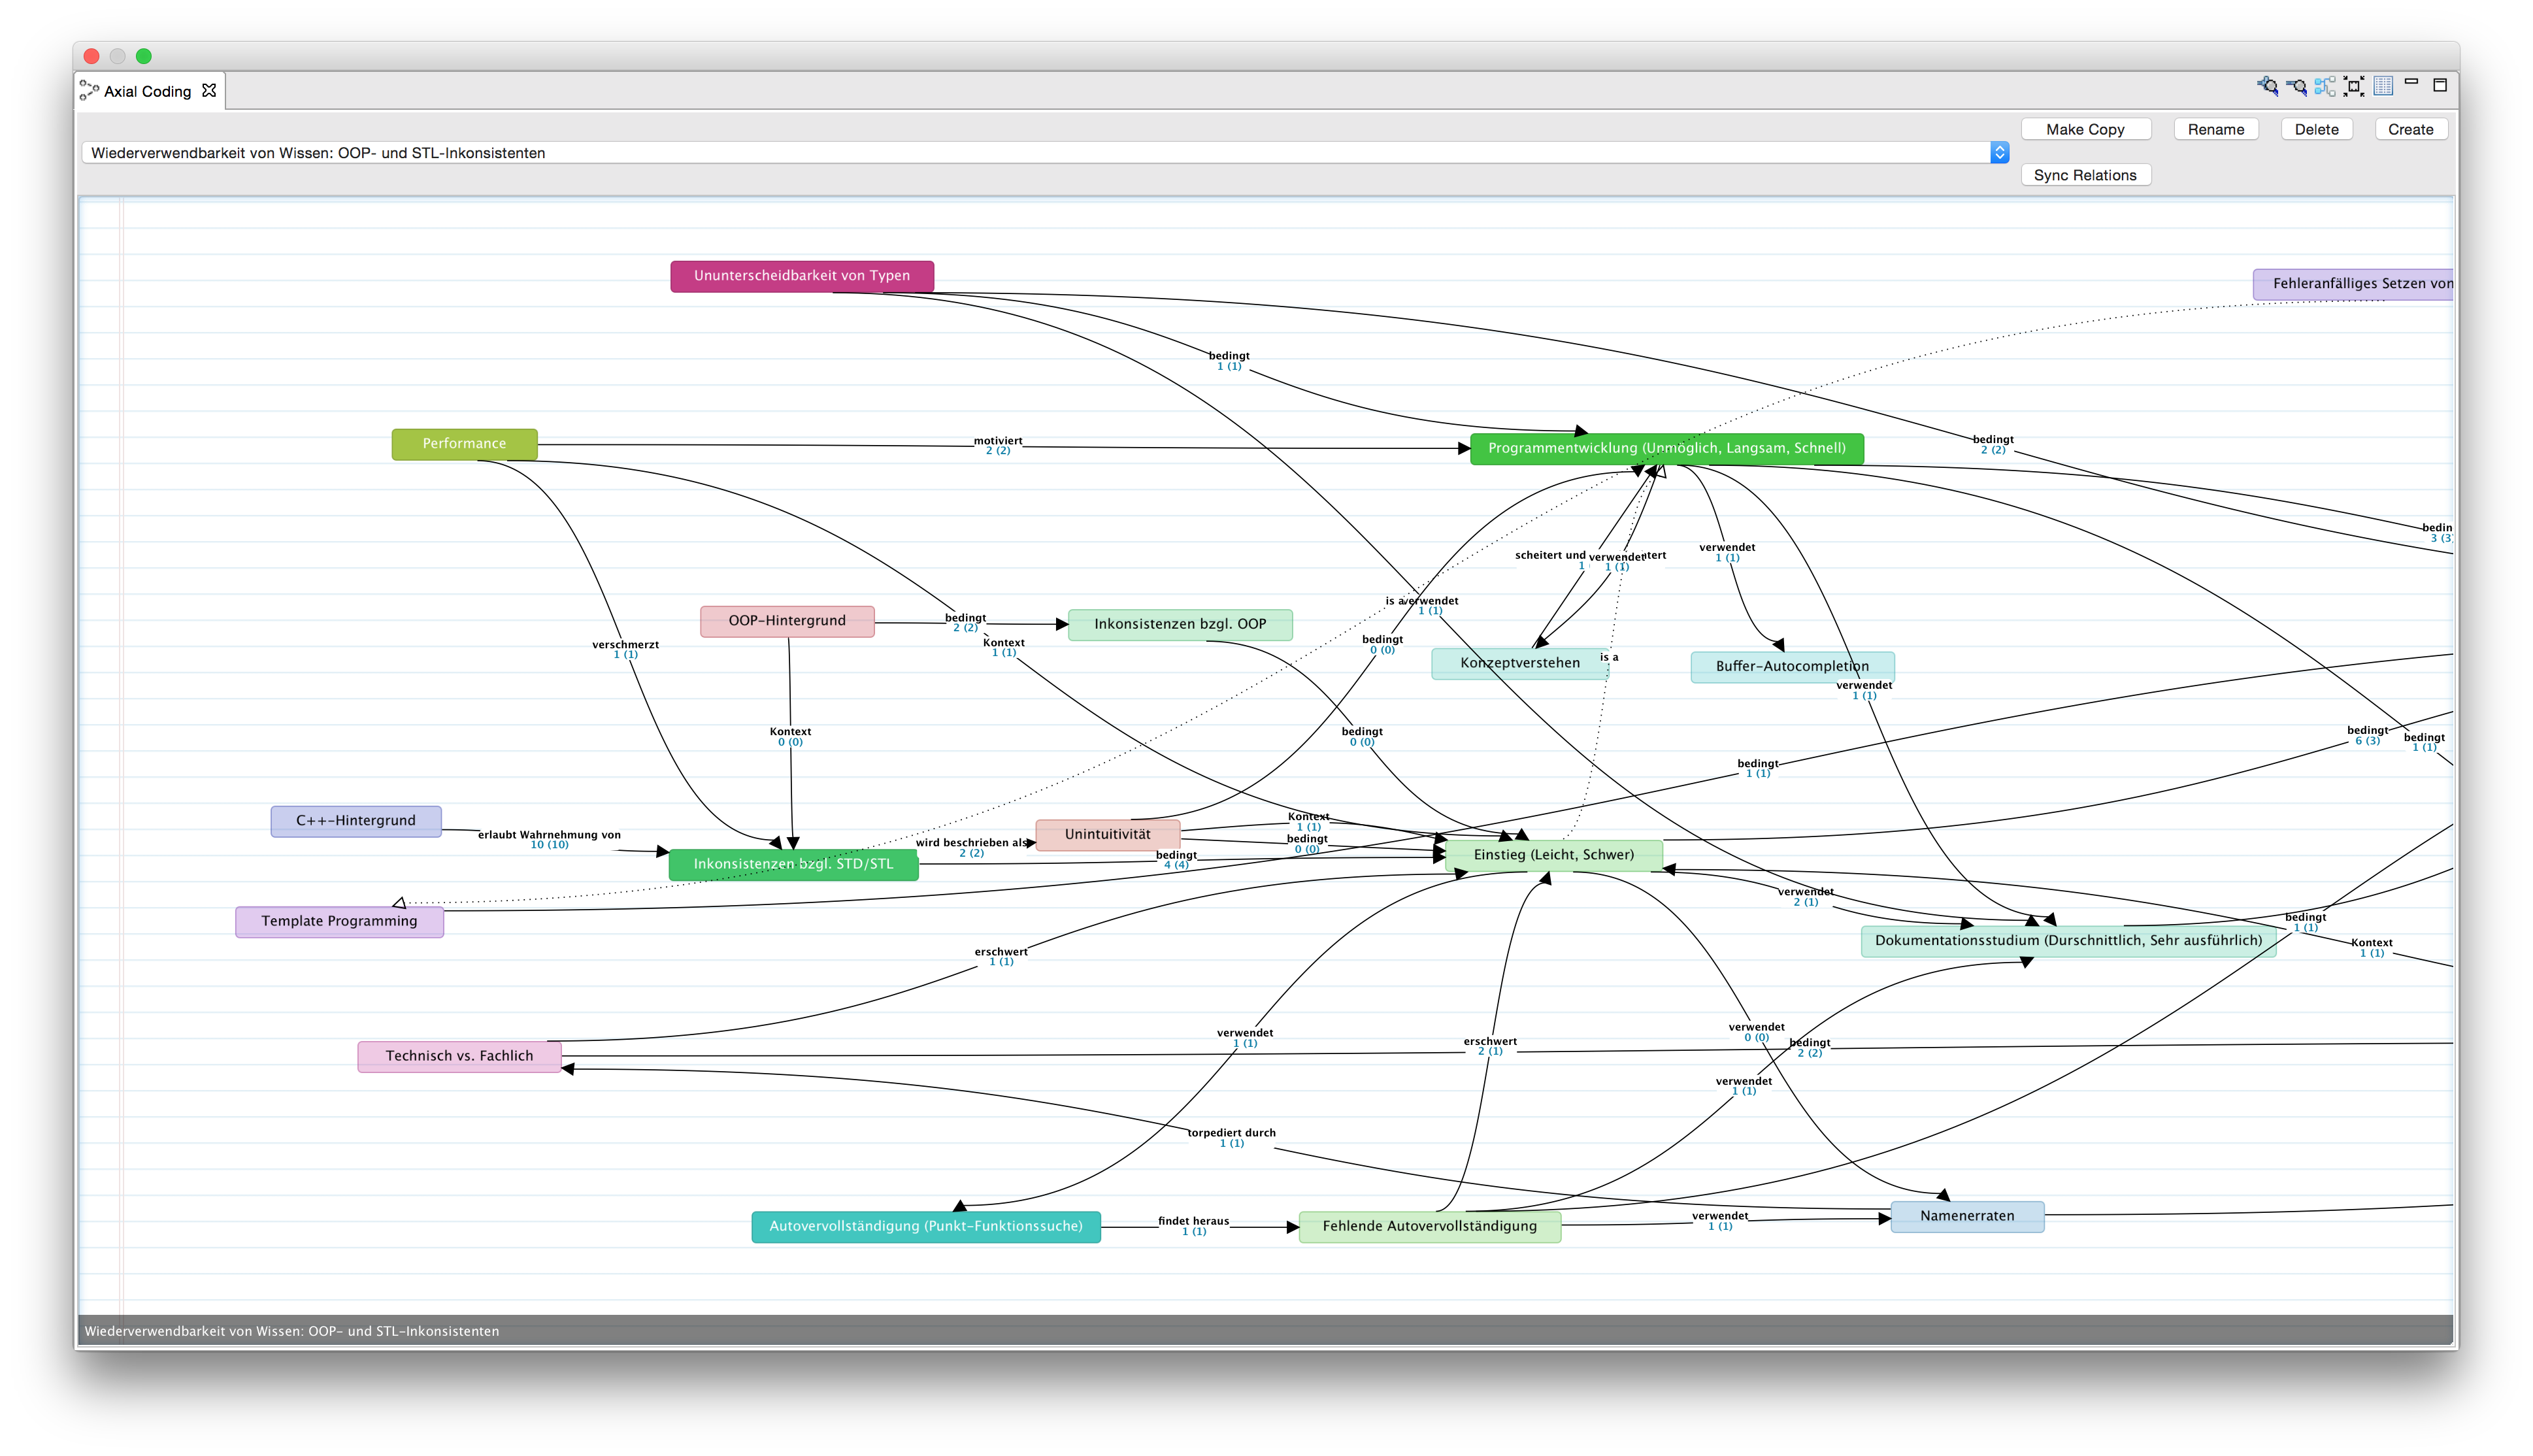
\includegraphics[width=1.0\linewidth]{Figures/acm/stl-inconcistencies-old.png}
  \caption{Axiale Kodierung des Konzepts \code{apiua://code/-9223372036854775633}}
  \label{fig:research-gt-vorlage}
\end{minipage}
\end{figure}

Ich stellte mir die Frage, worin sich \code{apiua://code/-9223372036854775633} und \code{apiua://code/-9223372036854775080} unterscheiden. Mir wurde plötzlich klar, dass die \code{apiua://code/-9223372036854775494}\footnote{Darunter verstehe ich einfach ausgedrückt, welche Paradigmen (objektorientierte Programmierung, Templatemetaprogrammierung, etc.) von einem Anwender auf Grund seiner Ausbildung oder Tätigkeit besonders präferiert und damit besonders gut beherrscht werden.} der Anwender eine elementare Rolle in der Bewertung der API-Usability spielt. In diesem Erklärungsansatz fühlte ich mich durch die Beobachtung bestätigt, dass sich der Gebrauch der Strategie \code{apiua://code/-9223372036854775145}\footnote{Darunter verstehe ich die Auflistung zur Verfügung stehender Funktionen durch die Eingabe eines Punktes nach einer Variablen innerhalb der eigenen IDE.} ebenfalls damit erklären ließ.

Abstrakt betrachtet, war allen Anwendern gemeinsam, dass sich die Usability von SeqAn signifikant aus den Vorerfahrungen und Vorkenntnissen seiner Anwender ergab, was ich als \textit{Erwartungskonformität} bezeichnet habe, und die Perspektive für  das selektive Kodieren darstellte.

Je mehr ich wichtige von weniger wichtigen Konzepten unterschied, desto deutlicher wurde, dass eine ganze Reihe von unempirischen \code{apiua://code/-9223372036854775281} ursächlich für die von mir beobachteten Usability-Probleme war.

Beim selektiven Kodieren habe ich ein ganzheitliches axiales Kodiermodell entwickelt\citepurl{apiua://axialcodingmodel/Yty2pVeMWuNS2BoX}, das durch einen sehr hohen Komplexitätsgrad gekennzeichnet war (siehe \fref{fig:research-gt1}). Um dieses in seiner Komplexität, aber dennoch sinnerhaltend zu reduzieren, entwickelte ich eine APIUA-Funktion, die es mir erlaubte, Relationen zu abstrahieren, d.h. entlang der Konzept-Hierarchien der verbundenen Konzepte nach oben zu bewegen. Ob es sich dabei um eine legitime Operation handelt, konnte ich durch die APIUA-Funktion der hypothetischen Relationen (siehe \sref{sec:Erkenntnisperspektive}) beantworten. Auf diese Weise konnte ich in dem Dickicht an gefundenen Relationen solche finden, die zusammengefasst und abstrahiert werden können.

Schienen hypothetische Relationen vollkommen unpassend, deutete dies auf Modellierungsschwächen hin. Beispielsweise waren die Folgen von \code{apiua://code/-9223372036854775514} (\code{apiua://code/-9223372036854775513} und \code{apiua://code/-9223372036854775511}) fälschlicherweise Unterkonzepte von \code{apiua://code/-9223372036854775514} selbst. Das Verschieben dieser Folgen in den anderen Teilbaum \code{apiua://code/-9223372036854775405} entsprach mehr der in den Daten manifesten Ordnung und reduzierte die Komplexität des zunehmend theoretischen Modells (siehe \fref{fig:research-workflow-selectivecoding-c}). Das Zwischenergebnis nach gut fünf Wochen aufwändigen selektiven Kodierens zeigt \fref{fig:research-gt2}\footnote{Leider kam das selektive Kodieren auf derart ungünstige Weise ins Stocken, dass ich die Diagnose und die Behebung des Problems im \aref{app:acm-editor-problem} ausführlicher beschreibe.}.

\begin{figure}
        \centering
        \begin{subfigure}{0.48\linewidth}
                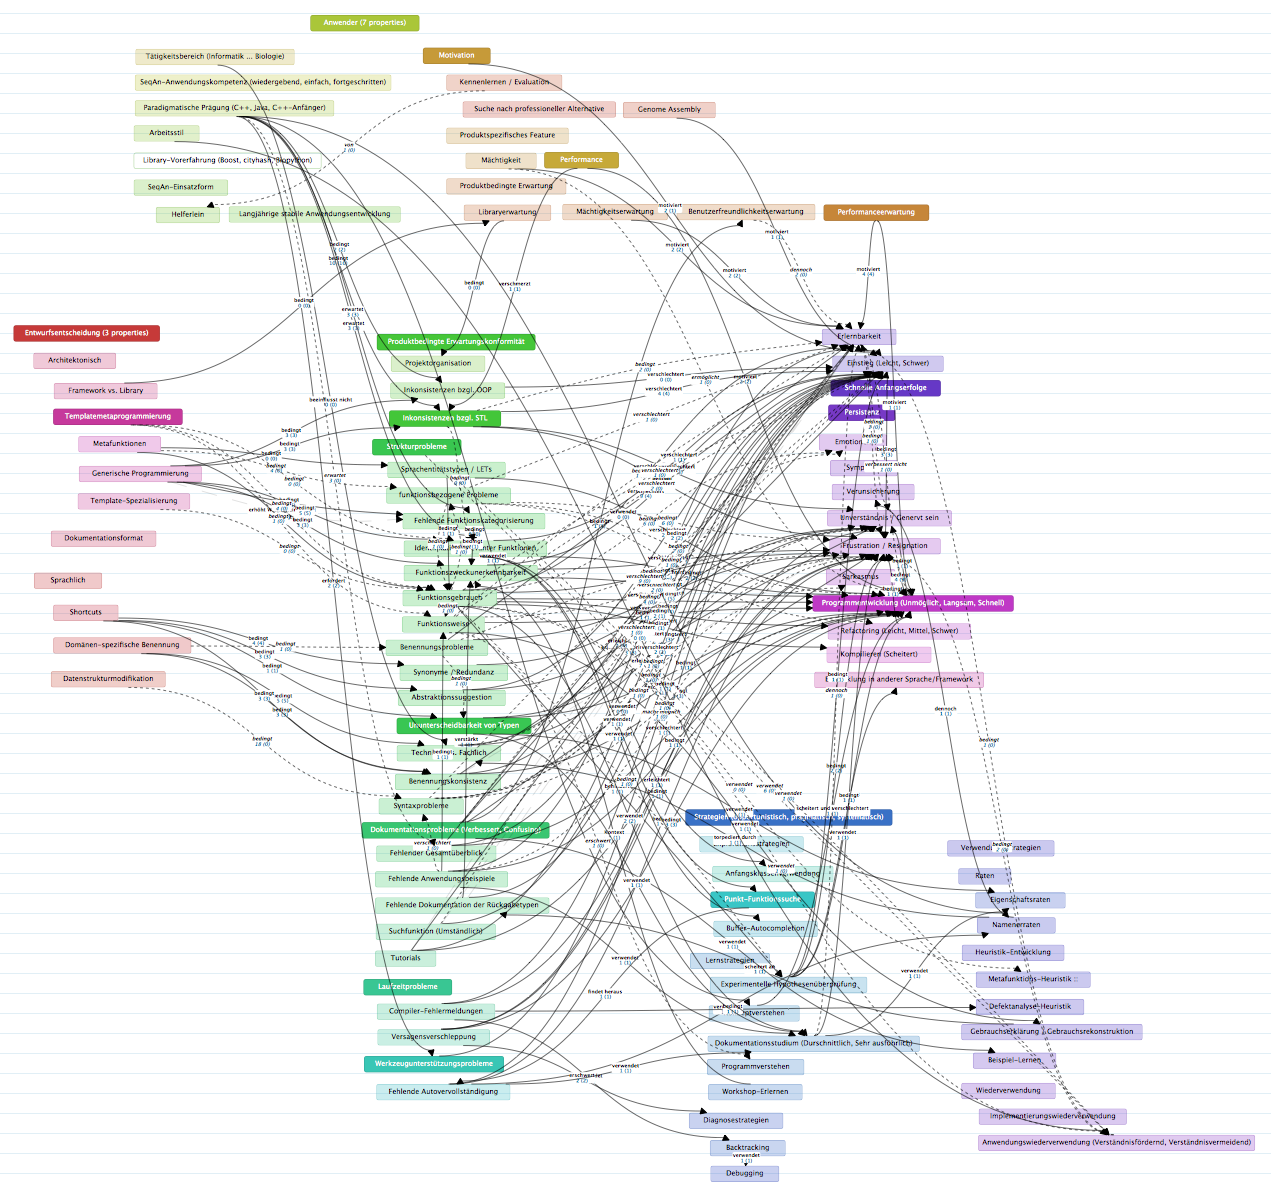
\includegraphics[width=\linewidth]{Figures/research/gt1.png}
                  \caption{Stand: 15.02.2015}
                \label{fig:research-gt1}
        \end{subfigure}%
        \hfill%
        \begin{subfigure}{0.48\linewidth}%
                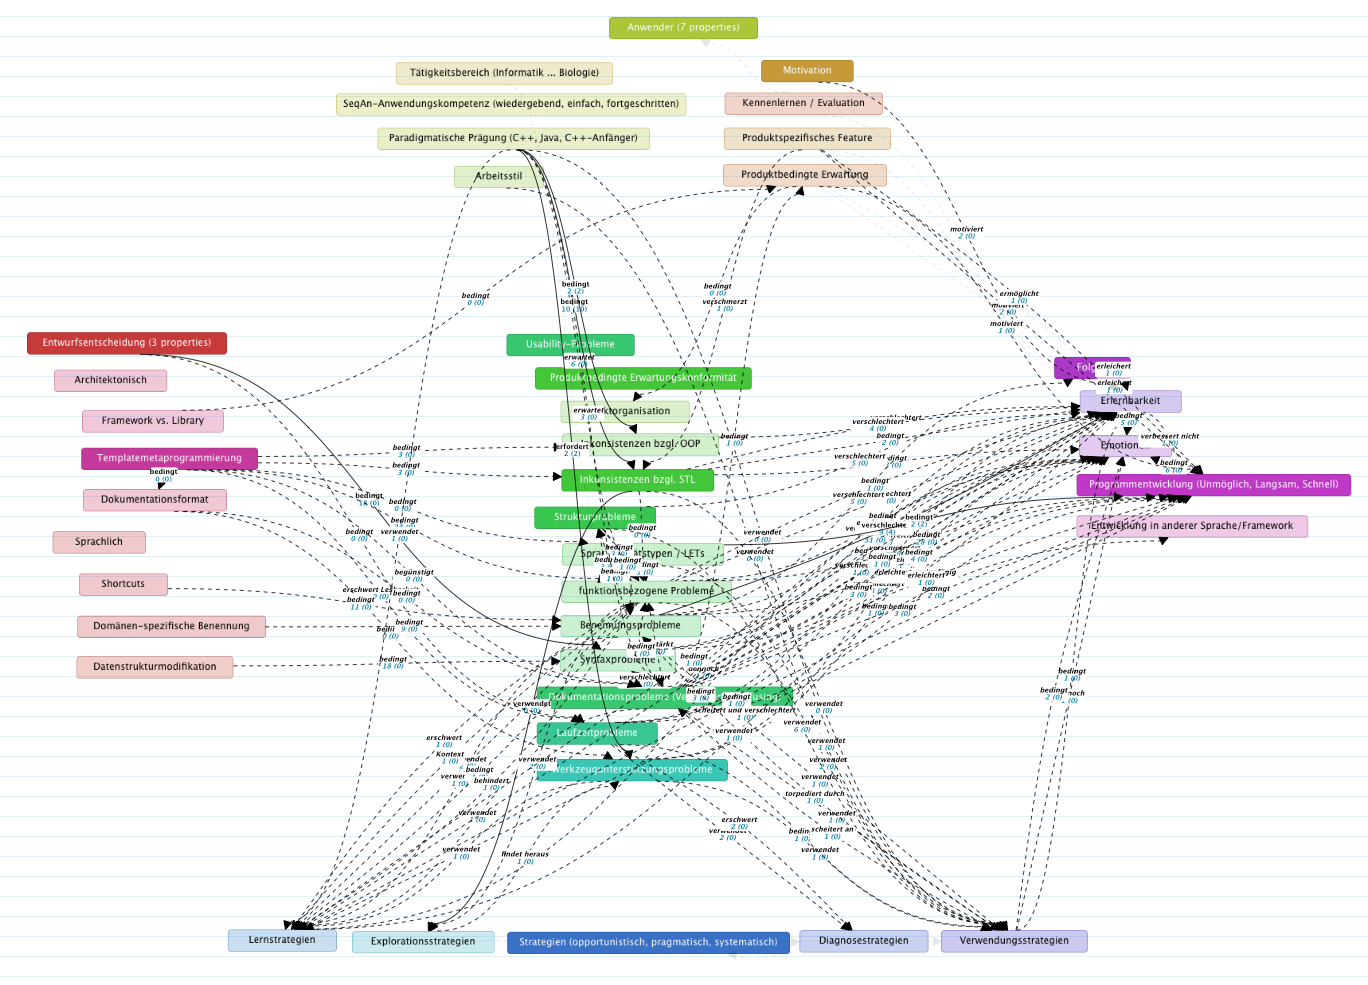
\includegraphics[width=\linewidth]{Figures/research/gt2.png}
                \caption{Stand: 24.03.2015}
                \label{fig:research-gt2}
        \end{subfigure}%
        \caption{Selektives Kodieren in APIUA}%
\end{figure}


\begin{figure}
        \centering
        \begin{subfigure}{0.43\linewidth}
                \includegraphics[width=\linewidth]{Figures/research/workflow-selectivecoding-a.png}
                  \caption{ohne Zusammenfassung von hypothetischen Relationen}
                \label{fig:research-workflow-selectivecoding-a}
        \end{subfigure}%
        \hfill%
        \begin{subfigure}{0.43\linewidth}%
                \includegraphics[width=\linewidth]{Figures/research/workflow-selectivecoding-b.png}
                \caption{mit Zusammenfassung von hypothetischen Relationen}
                \label{fig:research-workflow-selectivecoding-b}
        \end{subfigure}%
        \hfill%
        \begin{subfigure}{0.48\linewidth}%
                \includegraphics[width=\linewidth]{Figures/research/workflow-selectivecoding-c.png}
                \caption{nach dem Verschieben von zwei Konzepten}
                \label{fig:research-workflow-selectivecoding-c}
        \end{subfigure}%
        \caption{Selektives Kodieren in APIUA mit Hilfe zusammengefasster hypothetischer Relationen}%
        \label{fig:research-workflow-selectivecoding}
\end{figure}




\subsection{Probleme}

Neben den bereits genannten Problemen traten auch solche auf, die den Gebrauch der \gls{gtm} selbst betreffen. Drei Problemklassen stelle ich im Folgenden vor.


\subsubsection{Komplexität und Fokus}
\label{sec:schwierigkeiten-breite}

Empirische Forschungsmethode, zu denen die \gls{gtm} gehört, werden von \cite{SIGCHI:2009up} nur zu Evaluation eines einzelnen API-Aspektes als geeignet betrachtet. Das bestätigen auch andere Studien \citep[vgl. u.a.][]{Stylos:2008jt,Beaton:2008jn,Beaton:2008ix,Ellis:2007kv,Stylos:2007jb}. Ich habe versucht, SeqAn in seiner ganzen Breite zu betrachten, was eine Reihe von Aspekten --- angefangen bei der \code[apiua://code/-9223372036854774893]{Anwenderschaft} bis hin zu \code[apiua://code/-9223372036854775448]{Benennungsproblemen} --- umfasst. Meinen Anspruch, diese Breite in der gegebenen Zeit auch in der selben Tiefe zu betrachten, ist mir nicht vollständig gelungen, wie die Forschungsergebnisse zeigen werden. Darum hatte ich mich entschlossen, mich auf die \code{apiua://code/-9223372036854775515} und die Folgen der \code{apiua://code/-9223372036854775494}{paradigmatischen Prägung} zu konzentrieren, was sich beispielsweise in der geringen Entdeckung von Eigenschaften anderer Konzepte äußert.


\subsubsection{Modellierung der Ergebnisse}
\label{sec:gtm-modellierung}

Die Modellierung meiner Theorie fiel mir alles andere als leicht. Durch die \gls{apiua}-Unterstützung hierarchischer Konzepte stellte sich häufig die Frage, welches Kriterium als Zerlegungskriterium für Unterkonzepte verwendet werden soll und welche Kriterien als Eigenschaften dienen. Für meine Daten haben sich gleich fünf mögliche Konzepte gebildet, die als Elternkonzepte bzw. Zerlegungskriterium für die möglichen Unterkonzepte dienen konnten:

\begin{itemize}
  \item \code{Erwartungskonformität}\\Inwiefern kann existierendes Wissen durch den Anwender wiederverwendet werden?
  \item \code{apiua://code/-9223372036854774950}\\Welche kognitiven Dimensionen sind betroffen?
  \item \code{SeqAn-Feature}\\Mit welcher Funktionalität/Merkmal von SeqAn hat meine Beobachtung zu tun?
  \item \code{apiua://code/-9223372036854775281}\\Welche Art von Entwurfsentscheidung liegt vor?
  \item \code{apiua://code/-9223372036854774939}\\Was für eine Art Usability-Problem liegt vor?
\end{itemize}

Ich glaube, dass dieses Problem nicht nur mit meiner Unerfahrenheit im Gebrauch der \gls{gtm} und der Möglichkeit, Konzepte hierarchisch anzuordnen zu tun hat, sondern auch mit der geringen anwendungsbezogenen Strukturierung der GTM-Literatur \citep[insb.][]{strauss1990basics,strauss1987qualitative,glaser1978theoretical}. In der Dissertation von \cite{Salinger:2013vd} beschreibt der Autor ähnliche Probleme (S. 107 f.) und formuliert vier Praktiken, die ihm dabei halfen diese Probleme zu lösen (S. 108 ff.). Praktik 1 ``Blickwinkel auf die Daten'' hätte mein Modellierungsproblem sicherlich geschmälert, indem mir bewusster gewesen wäre, dass sich mein Blickwinkel auf die Daten ändert und welchen ich gerade habe.

Inhaltlich gesehen gibt es leider keine umfassenden API-Usability-Taxonomien \citep{Daughtry:2009be}, die meine Modellierung vereinfacht haben könnten. Allerdings konnte ich für das oben bereits genannte Konzept \code{apiua://code/-9223372036854775281} auf eine entsprechende Taxonomie von \cite{Stylos:2007ip} zurückgreifen. Taxonomien für Usability-Probleme werden von \cite{Khajouei:2011bm,Keenan:1999di} vorgeschlagen. Beide Taxonomien wurden empirisch, allerdings ausschließlich durch die Auswertung grafischer Benutzeroberflächen mit textuellen Komponenten entwickelt. Einzig \cite{Grill:2012jm} haben sich speziell mit API-Usability-Problemen befasst und für deren Unterteilung die vier Kategorien \textit{Dokumentation}, \textit{Laufzeit}, \textit{Struktur} und \textit{Benutzererlebnis} verwendet.

Ein weiteres Problem ist, dass bestimmte Werte für Eigenschaften gemeinsam mit dem Konzept wiederum ein Konzept bilden können. Beispiel: \code{apiua://code/-9223372036854775281} haben die Eigenschaft \code{apiua://code/-9223372036854774839}, welche die Ordinalskala \textit{(implizit, explizit-intuitiv, explizit-argumentativ, explizit-empirisch)} verwendet. Implizite und explizite-intuitive Entwurfsentscheidungen bilden in meiner Theorie das Konzept \code{Bauchgefühlentscheidung}. Inhaltlich ist das nachvollziehbar und kanonisch. Jedoch ist die technische Realisierung schwierig und führt zu einer weiteren Abstraktionsebene innerhalb einer \acrfull{gt}, weshalb ich diese Funktion nicht implementiert habe.

\label{sec:Datenanalyse-STL-Inkonsistenzen-vereinfachen}
Axiale Kodiermodelle können sehr groß werden, wie die \fref{fig:research-gc-acm} veranschaulicht. Solche Modellierungen auf das Wesentliche zu reduzieren, stellte mich vor große Probleme. Bei deren Reduktion halfen mir das APIUA-Werkzeug durch die Darstellung impliziter und hypothetischer Relationen, auf die ich im \sref{sec:Erkenntnisperspektive} auf Seite \pageref{sec:Erkenntnisperspektive} eingegangen bin.

\begin{figure}
\begin{minipage}{\textwidth}
  \centering
    \includegraphics[width=1.0\linewidth]{Figures/research/gc-acm.png}
  \caption[Axiales Kodiermodell zur Gruppendiskussion]{Axiales Kodiermodell zur Gruppendiskussion\citepurl{apiua://axialcodingmodel/0z5ANneuBKhFKJkb}}
  \label{fig:research-gc-acm}
\end{minipage}
\end{figure}




\subsubsection{Validität}
\label{sec:probleme-validierung}

Während die Programmierfortschritte-Daten in situ sind, handelt es sich bei den Cognitive-Dimensions-Fragebögen um Ex-post-facto-Daten, die eine andere Perspektive für die axiale Kodierung im Sinne des paradigmatischen Modells erfordern. Darüber musste ich mir erst durch mehrere Analyseanläufe bewusst werden. Das betrifft insbesondere das axiale Kodieren von mehr als einem Fragebogen: Lässt sich beispielsweise in einem Fragebogen die Relation \rel[]{\code{apiua://code/-9223372036854774928}}{\code{apiua://code/-9223372036854774927}} und in einem anderem Fragebogen die Relation \rel[]{\code{apiua://code/-9223372036854774927}}{\code{apiua://code/-9223372036854774926}} finden, kann daraus nicht ohne Weiteres auf einen Zusammenhang \rel[]{\code{apiua://code/-9223372036854774928}}{\code{apiua://code/-9223372036854774926}} geschlossen werden. Dazu würde ein gutes Verständnis vom Kontext vorliegen müssen, der den Fragebögen häufig aber kaum zu entnehmen ist.

Im Gegensatz zu den Programmierfortschritte-Daten, sind die subjektiven Datenquellen häufig ärmer an Kontextinformationen. Beide Datenquellen waren aber überraschend breit in ihrem Aussagegehalt, was dazu führte, dass ich viele Konzepte entdecken, aber nur wenige Verankerungen/Phänomene dazu finden konnte.
% Aus Zeitgründen, konnte ich nicht jedes Konzept in den Programmierfortschritte-Daten suchen und damit triangulieren
Dies führte mich zu der Frage, welche Aussagekraft überhaupt die Anzahl der zu einem Konzept gefundenen Phänomene haben. In einer \gls{gtm} der zweiten Generation \citep{charmaz2006constructing} können textuelle Daten explizit Wort-, Zeilen- und Absatz-weise kodiert werden, was massiven Einfluss auf die Anzahl gefundener Phänomene hat. Entsprechend eignet sich dieses quantitative Maß nur bedingt nur Diskussion der Validität.




\begin{comment}

\subsection{Anekdoten}
%TODO schreiben am Ende
In diesem letzten Abschnitt möchte ich an Hand konkreter Beispiele darstellen, wie ich die \gls{gtm} angewendet und inwieweit sie mir beim Erkenntnisgewinn und der Generierung einer validen \gls{gt} geholfen hat.


\subsubsection{Vorteile qualitativen Forschung}
- 3 Phänomene mit Code "Mächtigkeit" kodiert
- Phänomene waren Antworten auf die Frage nach der Work-Step Unit von SeqAn
- Erkenntnis: SeqAn bekommt durch die 3 Teilnehmer eine gute WSU bescheinigt bekommen
- schließlich war der Fragebogen mit großer Sorgfalt und basierend auf dem von Green und Clarke (Ausrichtung nach API) entworfen worden
- ABER: stimmt die Erkenntnis?
- Die 3 befragten waren Teilnehmer der Workshops
- Alle hatten mit SeqAn nur Kontakt innerhalb des Workshops und dabei vornehmlich Tutorials bearbeitet
- Folge: Sie konnten die Frage nicht adäquat beantworten. Stattdessen haben Sie (unbewusst) Äußerungen zu dem gemacht, was sie sich von SeqAn versprechen (aus irgendeinem grund müssen sie ja beim Workshop sein)
- Der Code heißt nun Mächtigkeitseindruck apiua://code/-9223372036854775568
- abstraktives Fazit: Das die Anwendungsdauer auf die Interpretation der anderen Antworten Auswirkungen hat, kann man nur qualitativ herausfinden


\subsubsection{Paraphrasierung und wortgenaue Analyse}
Wortgenaue Analyse: \citep{charmaz2006constructing}
Annekdote Paraphrasierung und wortgenaue Analyse (gelernt im Seminar)
- ~hilft den Kern einer Aussage zu erfassen
- kann aber auch helfen, eine Aussage erst auswerten zu können (aufgrund der fehlenden Klammerung in der Sprache zum Beispiel)

- Aussage apiua://survey/cd/2013-09-19T11:51:16.616+02:00/hardMentalOperations:
Yes, remembering all the templates and variants of types and templates and trying to figure out what is the difference between say Dna5 and Dna5String.

Remembering bezieht sich klar auf templates und variants. Aber bezieht sich variants auch auf type and templates oder nur auf type und "and templates" ist ein dritter Aufzählungspunkt (Sprache ist nicht immer perfekt).
Also:

Stichpunktartige Paraphrase:
- remembering complicated
-- many templates
-- many variants of types
-- many variants of templates
- difference unclear
-- e.g. Dna5 and Dna5String

Kodierung
> Fachliche Inkorrektheit, apiua://code/-9223372036854775335
"many variants of types', 'Dna5 and Dna5String"

> Metafunktionen, apiua://code/-9223372036854775514
'many templates", Das Konzept Metafunktion selbst is neu/umfangreich.

> Typing, apiua://code/-9223372036854775352
'many variants of types and templates"
~ umfasst nämlich Metafunctionsaufrund die Angabe von Typen



Sehr gutes Beispiel in apiua://survey/cd/2013-09-19T11:51:16.616+02:00/hardMentalOperations



\subsubsection{Ständiges Vergleichen}
- ACM verwendet, um fehlende Relation zu finden.
Beispiel Group Discussion ACM
Bild: missing\_relations.png
Code Konventionen hatte keine ausgehende Relation 
Alle Citations geprüft und mit "erschwert Einstieg" nachkodiert



\subsubsection{Annekdote für Kompetezaufbau / theoretische Sensibilität / zu klären}
- Antwort auf die Frage nach der Viscocity von SeqAn (apiua://survey/cd/2013-09-18T17:50:13.425+02:00/viscosity)
"Wenn es wenig Beispiele gibt bzw. die Funktionalitaet mancher Konstrukte zu ergruenden ist"
- unklare Aussage
- Progressive Evaluation-Frage an anderen Teilnehmer apiua://survey/cd/2013-09-18T17:50:13.425+02:00/progressiveEvaluation: "Wenn man lange nach bestimmten Funktionen sucht bzw. lange braucht deren Verwendung zu verstehen ist der Fortschritt manchmal schwer zu ueberblicken."
- Hier wurde klar, was der andere mit "Funktionalitaet" meinte: Nämlich "Funktionsweise"


\subsubsection{Vereinfachung}
Annekdote für Minimalismus-Drang:
- Frage nach Cd-Work Step Unit
- Sehr viel. Aber ich denke wenig Code ist auch nicht immer die beste Lösung.
Bei seqAn finde ich es etwas zu wenig, da ich als Anfänger die Schritte nicht sehe die in einer Zeile stecken und es mir dadurch schwer fällt nachzuvollziehen was hier genau passiert.
- Ursprünglich kodiert als "Nachvollziehbarkeit".
- Später nochmal gesamten Fragebogen gelesen. User beklagt sich über technische Verständnisschwierigkeiten in anderen Fragen (z.B. keine Dokumentation der Rückgabetypen.
- Überlegung, ob nicht doch nur C++-Sprachkenntnisse fehlen
- ABER: In Frage nach Premature Commitment wird Generizität globaler Funktionen gelobt $\rightarrow$ also doch Kenntnisse
- Die Work-Step-Unit ist tatsächlich zu groß.Der Code bleibt "Nachvollziehbarkeit" oder so ähnlich (apiua://survey/cd/2013-09-18T17:45:54.889+02:00/workStepUnit)



\subsubsection{Verständnisschwierigkeiten (schlechtes Englisch)}
Aussage von apiua://survey/cd/2013-09-18T17:50:37.900+02:00/hardMentalOperations
Verschiedene Lesarten für "I feel that you need to get use to available functions to make things work.":
1. Ich muss mich erst an die vorhandene Funktionalität gewöhnen.
2. Ich muss erst verstehen, welchen Funktionen überhaupt bereit stehen.

Entscheidung in Anbetracht seines in den anderen Fragen geäußerten Kenntnissstandes (bloody beginner): 1



\subsubsection{Voreingenommenheit}
- Aussage zur Work-Step Unit Frage: apiua://survey/cd/2013-09-18T17:45:54.889+02:00/workStepUnit: 
- Kodierung: "Verständnis Funktionsweise" mit Wert "Abstrahiert", Memo: "Abstrahiert: Der Grad der Abstraktion verbirgt die einzelnen Ausführungsschritte, was das Verständnis erschwert.
Möglich Ursache: Zu große Work-Step Unit"
- Erst mit der Aussage apiua://survey/cd/2013-09-18T17:45:54.889+02:00/roleExpressiveness wurde klar, dass in beiden Fällen die Strategie beschrieben wird, wird der Befragte mit fehlenden (oder unzureichenden / unpassenden) Anwendungsbeispielen umgeht. Er erklärt sich die Anwendung dann mit dem Funktionsablauf und der Rückgabe. siehe apiua://code/-9223372036854775401, mit Work-Step Unit hat das herzlich wenig zu tun oder höchstens insoweit, als dass sie das Problem hier abgeschwächt hätte


\subsubsection{Soziale Erwünschheit und Vorbelastung}
apiua://survey/cd/2013-09-18T17:46:55.042+02:00/learningStyle sagt die Tutorials seien hilfreich; sagt aber auch "zum größten Teil" und schränkt im folgenden Satz weiter ein.
Die Tutorials wurden von mir überarbeitet. Erst der Blick durch eine zweite Person brachte diese neue Perspektive.



\subsubsection{Theoretisches Sampling}
- zeigt, wie Reichhaltig die Daten sind und sind ein Qualitätsmerkmal für meine Art der Datenerhebung
Annektode Existierende Quellen nochmals sichten:
Manchmal und gerade am Anfang sieht man bestimmte Aspekte einer Aussage nicht. Man ist für sie blind. Erst wenn man die notwendige Sensibilität und/oder einem dieser Aspekt auf dem Silbertablett präsentiert wird, muss man in sein bereits kodiertes Material zurückkehren und Phänomene für diesen Aspekt suchen.
Geschehen bei apiua://code/-9223372036854775314 - Frustation. Aufmerksam geworden bei "99\% of the cases when I refactor something first version will not even compile." apiua://survey/cd/2013-09-19T11:51:16.616+02:00/viscosity und dann auch Dinge wie "Meistens lassen sich Dinge nicht überprüfen, weil der Code nicht kompiliert. Das Prototypen von Dingen fällt mir oft sehr schwer." apiua://survey/cd/2013-09-18T17:46:55.042+02:00/progressiveEvaluation dessen Frustration man sehr gut im Kontext seiner anderen Antworten (wiederholt "schwer", "sehr schwer", "nicht leicht") sehen kann 


\subsubsection{Reliabilität}
- ein drei Wochen alte Quelle apiua://survey/cd/2013-09-19T11:51:16.616+02:00/workStepUnit ein drittes Mal kodiert (ohne auf alte Codes zu schauen)
- erst: Glaube, als gefunden Codes bereits gefunden zu haben.
- dann: ein neuer Code; noch einmal überlegt. Nein, dieser neue Code ''Overhead`` ist nur ein Aspekt von Work-Step Unit (TP erfordert die Berechnung von Typen und macht damit Ausdrücke syntaktisch komplexer - länger als ohne)
- Vergessene Codierschritte exakt identisch gemacht, sogar gleiche Zitate rausschreiben wollen
=> gutes Zeichen



\subsubsection{Refactoring}
-apiua://survey/cd/2013-09-18T17:45:54.889+02:00/hardMentalOperations
"Hard Mental Operations: Eingentlich nicht. Es braucht sicher etwas Übung. Aber dafür sind die guten Assignments sehr Hilfreich."
Bisher kodiert als "Lernfortschritt mittels Assignment"
Dann wurde aber klar, dass es sich um zwei Formen handelt:
1. Die Bearbeitung der Assignments im Rahmen der Bearbeitung von Tutorials (TODO: Code nennen)
2. Eine Strategie, die eingesetzt wird, sobald die Programmentwicklung ins Stocken gerät (TODO: Code nennen)

\end{comment}











%Allgemein:
%Exakte GT - insbesondere mit der Modellierung von Eigenschaften - bei der Fülle an Bedienungsproblemen äußerst komplex. Man müsste entweder erheblich mehr Zeit investieren, oder die Betrachtungsbreite einschränken.
%Daher Clustering-Ansatz gewählt, bei dem Codes gruppiert sind (und damit implizit Eigenschaften enthält).
%Beispiel:
%Professionelle Programmentwicklung, Einstieg, Herumprobieren könnten alle der Code Programmentwicklung mit den Eigenschaften Zweck/Ziel (Produktion, Erlernen) und Temporalität (Persistent, Temporär) sein. Professionelle Programmentwicklung wäre dann Produktion+Persistent, Einstieg (Erlernen+Persistent) und Herumprobieren (Erlernen, Temporär)

%Vereinfachtes axiales Kodieren:
%Paradigmatisches Modell, das wie eine visuelle Schablone (TODO Grafik) gelesen werden soll.
%Umdefinition von Kontext: Alle Konzepte, die das interpretatorische Bild vervollständigen (Hintergrundinformationen,
%die Einfluss haben können) (also nicht: Eigenschaften-Auswahl von XXX und Ursache)
%Umdefinition von XXX: Alle Konzepte, die belegt Einfluss auf zentrales Phänomen haben. 



\subsection{Zusammenfassung}

In dieser Phase 4 habe die eigentliche Forschung mit Hilfe der \gls{gtm} und meinem Datenanalysewerkzeug \gls{apiua} besprochen. Dazu habe ich zunächst die Forschungsmethoden anderer Studien vorgestellt. Dabei bin ich auf die Eignung und die seltene Verwendung der \gls{gtm} für explorative Studien eingegangen. Ich habe den unterschiedlichen Gebrauch der \gls{he} erläutert und bin auf die Schwächen anderer Forschungsmethoden eingegangen.

Anschließend habe ich die Analyse der Programmierfortschritte-Daten, der Cognitive-Dimensions-Fragebögen und der Gruppendiskussion beispielhaft skizziert und die konkrete Umsetzung innerhalb von \gls{apiua} dargestellt.

In meiner Beschreibung des selektiven Kodierens, habe ich erläutert, welchen Beitrag die Konzepte \code{apiua://code/-9223372036854775633} und \code{apiua://code/-9223372036854775494} beim Durchbruch meiner Forschung hatten und welche APIUA-Funktionen mir bei der Reduktion des ``globalen'' axialen Kodiermodells auf ein theoretisches Kodiermodell behilflich waren.

Weiterhin bin ich auf Komplexitäts-, Modellierungs- und Validitätsprobleme beim Gebrauch der \gls{gtm} eingegangen.% und habe meine Forschungsgenauigkeit anekdotisch beschrieben.



\section{Zusammenfassung der Forschung}

In diesem Kapitel habe ich die Erforschung der API-Usability von SeqAn vorgestellt. Dazu bin ich zunächst auf die Rahmenbedingungen, sowie auf die ursprünglich geplante und die tatsächlich durchgeführte Forschung eingegangen.

In Phase 1 habe ich die Notwendigkeit und Durchführung der Beseitigung grober SeqAn-Usability-Probleme beschrieben. Dazu habe ich verschiedene Datenerhebungsverfahren (Online-Umfrage, Interviews, Feedback) und eine vereinfachte Evaluation mit Hilfe der \glslink{he}{Heuristischen Evaluation} durchgeführt.

In Phase 2 habe ich die Planung und Durchführung der für meine Forschung notwendigen Datenerhebung erläutert. Eingegangen bin ich dabei auf die Gruppendiskussion, auf den eigens für die Evaluation von APIs entwickelten Cogntive-Dimensions-Fragebogen und das neuartige Programmierfortschritte-Datenerhebungsverfahren.

Phase 3 beschäftigt sich mit dem qualtativen Datenanalysewerkzeug \gls{apiua}, dessen Entwicklung die spezielle Datenerhebung in Verbindung mit der \gls{gtm} erforderte.

Schließlich stellte ich in Phase 4 die Analyse der erhobenen Daten mit Hilfe der \gls{gtm} und des Datenanalysewerkzeugs vor.

\bigskip

In dem folgenden Kapitel präsentiere ich meine eigentlichen Forschungsergebnisse.

\cleardoublepage